\documentclass[12pt,a4paper,]{report}
\usepackage{lmodern}

% MP: set font to helvetica (basically free arial) and margin size to 1.
\usepackage{geometry}
\geometry{a4paper, portrait, twoside, margin=1in, inner=1.57in}
\usepackage{helvet}
\renewcommand{\familydefault}{\sfdefault}

% Overwrite \begin{figure}[htbp] with \begin{figure}[H]
\usepackage{float}
\let\origfigure=\figure
\let\endorigfigure=\endfigure
\renewenvironment{figure}[1][2] {
    \expandafter\origfigure\expandafter[H]
} {
    \endorigfigure
}

% fix for pandoc 1.14
\providecommand{\tightlist}{%
  \setlength{\itemsep}{0pt}\setlength{\parskip}{0pt}}

% TP: hack to truncate list of figures/tables.
\usepackage{truncate}
\usepackage{caption}

% MP: make figure labels bold
\captionsetup{labelfont=bf}

% MP: packages for abbrv. list table
\usepackage{longtable}
\usepackage{datatool}
\usepackage{booktabs}

\usepackage{tocloft}
% TP: end hack

\usepackage{setspace}
\doublespacing

\usepackage{amssymb,amsmath}
\usepackage{ifxetex,ifluatex}
\usepackage{fixltx2e} % provides \textsubscript
\ifnum 0\ifxetex 1\fi\ifluatex 1\fi=0 % if pdftex
  \usepackage[T1]{fontenc}
  \usepackage[utf8]{inputenc}
\else % if luatex or xelatex
  \ifxetex
    \usepackage{mathspec}
    \usepackage{xltxtra,xunicode}
  \else
    \usepackage{fontspec}
  \fi
  \defaultfontfeatures{Mapping=tex-text,Scale=MatchLowercase}
  \newcommand{\euro}{€}
\fi
% use upquote if available, for straight quotes in verbatim environments
\IfFileExists{upquote.sty}{\usepackage{upquote}}{}
% use microtype if available
\IfFileExists{microtype.sty}{%
\usepackage{microtype}
\UseMicrotypeSet[protrusion]{basicmath} % disable protrusion for tt fonts
}{}
\usepackage{color}
\usepackage{fancyvrb}
\newcommand{\VerbBar}{|}
\newcommand{\VERB}{\Verb[commandchars=\\\{\}]}
\DefineVerbatimEnvironment{Highlighting}{Verbatim}{commandchars=\\\{\}}
% Add ',fontsize=\small' for more characters per line
\newenvironment{Shaded}{}{}
\newcommand{\AlertTok}[1]{\textcolor[rgb]{1.00,0.00,0.00}{\textbf{#1}}}
\newcommand{\AnnotationTok}[1]{\textcolor[rgb]{0.38,0.63,0.69}{\textbf{\textit{#1}}}}
\newcommand{\AttributeTok}[1]{\textcolor[rgb]{0.49,0.56,0.16}{#1}}
\newcommand{\BaseNTok}[1]{\textcolor[rgb]{0.25,0.63,0.44}{#1}}
\newcommand{\BuiltInTok}[1]{#1}
\newcommand{\CharTok}[1]{\textcolor[rgb]{0.25,0.44,0.63}{#1}}
\newcommand{\CommentTok}[1]{\textcolor[rgb]{0.38,0.63,0.69}{\textit{#1}}}
\newcommand{\CommentVarTok}[1]{\textcolor[rgb]{0.38,0.63,0.69}{\textbf{\textit{#1}}}}
\newcommand{\ConstantTok}[1]{\textcolor[rgb]{0.53,0.00,0.00}{#1}}
\newcommand{\ControlFlowTok}[1]{\textcolor[rgb]{0.00,0.44,0.13}{\textbf{#1}}}
\newcommand{\DataTypeTok}[1]{\textcolor[rgb]{0.56,0.13,0.00}{#1}}
\newcommand{\DecValTok}[1]{\textcolor[rgb]{0.25,0.63,0.44}{#1}}
\newcommand{\DocumentationTok}[1]{\textcolor[rgb]{0.73,0.13,0.13}{\textit{#1}}}
\newcommand{\ErrorTok}[1]{\textcolor[rgb]{1.00,0.00,0.00}{\textbf{#1}}}
\newcommand{\ExtensionTok}[1]{#1}
\newcommand{\FloatTok}[1]{\textcolor[rgb]{0.25,0.63,0.44}{#1}}
\newcommand{\FunctionTok}[1]{\textcolor[rgb]{0.02,0.16,0.49}{#1}}
\newcommand{\ImportTok}[1]{#1}
\newcommand{\InformationTok}[1]{\textcolor[rgb]{0.38,0.63,0.69}{\textbf{\textit{#1}}}}
\newcommand{\KeywordTok}[1]{\textcolor[rgb]{0.00,0.44,0.13}{\textbf{#1}}}
\newcommand{\NormalTok}[1]{#1}
\newcommand{\OperatorTok}[1]{\textcolor[rgb]{0.40,0.40,0.40}{#1}}
\newcommand{\OtherTok}[1]{\textcolor[rgb]{0.00,0.44,0.13}{#1}}
\newcommand{\PreprocessorTok}[1]{\textcolor[rgb]{0.74,0.48,0.00}{#1}}
\newcommand{\RegionMarkerTok}[1]{#1}
\newcommand{\SpecialCharTok}[1]{\textcolor[rgb]{0.25,0.44,0.63}{#1}}
\newcommand{\SpecialStringTok}[1]{\textcolor[rgb]{0.73,0.40,0.53}{#1}}
\newcommand{\StringTok}[1]{\textcolor[rgb]{0.25,0.44,0.63}{#1}}
\newcommand{\VariableTok}[1]{\textcolor[rgb]{0.10,0.09,0.49}{#1}}
\newcommand{\VerbatimStringTok}[1]{\textcolor[rgb]{0.25,0.44,0.63}{#1}}
\newcommand{\WarningTok}[1]{\textcolor[rgb]{0.38,0.63,0.69}{\textbf{\textit{#1}}}}
\ifxetex
  \usepackage[setpagesize=false, % page size defined by xetex
              unicode=false, % unicode breaks when used with xetex
              xetex]{hyperref}
\else
  \usepackage[unicode=true]{hyperref}
\fi
\hypersetup{breaklinks=true,
            bookmarks=true,
            pdfauthor={},
            pdftitle={},
            colorlinks=true,
            citecolor=black,
            urlcolor=black,
            linkcolor=black,
            pdfborder={0 0 0}}
\urlstyle{same}  % don't use monospace font for urls
\setlength{\parindent}{0pt}
\setlength{\parskip}{6pt plus 2pt minus 1pt}
\setlength{\emergencystretch}{3em}  % prevent overfull lines
\setcounter{secnumdepth}{5}

\date{}

\begin{document}

\begin{titlepage}
    \begin{center}

        
\includegraphics[width=0.4\textwidth]{title_pages/imgs/uos_logo_colour.png}
        
        \vspace*{2.5cm}
        
        \huge
        G-Quadruplexes and Gene Expression in \textit{Arabidopsis thaliana}
        
        \vspace{1.5cm}
        
        \normalsize
        By:
        \Large
        Matthew Parker, BSc

        \vspace{1.5cm}

        \normalsize
        A thesis submitted in partial fulfilment of the requirements for the degree of\\
Doctor of Philosophy 

        
        \vfill
        
        \normalsize
        The University of Sheffield\\
        Faculty of Science\\
        Department of Molecular Biology and Biotechnology\\

        \vspace{0.8cm}
        
        \normalsize
        \today


    \end{center}
\end{titlepage}

\newpage

\section*{Acknowledgements} 
\addcontentsline{toc}{chapter}{Acknowledgements}{}

Firstly I would like to thank my supervisor, Karim Sorefan, for guiding
me through the project, but also allowing me to take it in the
directions I wanted to go, i.e.~away from the bench, out of the lab
door, and towards the computer! Thanks also to Ian Sudbery for his
guidance in the world of bioinformatics, and for allowing me to join his
lab's meetings and journal club, without which I would have been stuck
with only the wet lab biologists for company. Also thanks to Marta Milo
who has helped me with a number of statistics problems over the last
four years, and Stuart Casson, for asking good questions in lab
meetings. I'd also like to thank Jeremy Craven, whose Python course,
which I took at undergraduate level, was what first got me hooked on
programming and bioinformatics.

From the Sorefan and Casson labs there are many people to thank.
Firstly, Colette Baxter, Manoj Valluru, Giulia Arsuffi, Nick Zoulias,
who between them did all of the wet lab experiments which provided me
with data to analyse. Colette's RNAseq data was of particularly high
quality (so many FDRs \textless{} 0.05!). Secondly, to James Thackery,
for being a ridiculously handsome devil and a hilarious human being;
Matthew Proctor, for being neither (just kidding); and Rachel Denley
Bowers, for taking me the the hospital at Peter Venn's wedding (Colette
also helped out there).

Finally I'd like to thank Catherine Heath, for putting up with me
chatting about bioinformatics when she clearly wasn't interested, and
for generally making my life pretty wonderful.

\newpage
\section*{Abstract} 
\addcontentsline{toc}{chapter}{Abstract}{}

G-Quadruplexes (G4s) are four stranded DNA structures which form in
regions with high GC content and high GC skew. Because of the dependence
of G4 structure on specific sequences, it is possible to predict
putative G4s (PG4s) throughout genomic sequence. PG4s are non-uniformly
distributed in genomes, with higher densities within various genic
features, particularly promoters, 5' untranslated regions (UTRs) and
coding sequences (CDSs). When they form G4s, these sequences can have a
variety of implications for biological processes including replication,
transcription, translation and splicing. Here, we introduce a novel
method for identifying PG4s, which uses a machine learning approach
trained on datasets derived from the high throughput sequencing of G4
structures. We apply this and other techniques, to study the prevalence
of PG4s in the genome of \emph{Arabidopsis thaliana}, the model plant.
Finally, we study the effect of G4 stabilisation using the G-Quadruplex
binding agent NMM on gene expression in Arabidopsis. We identify a
family of genes which are strongly downregulated by NMM, and find that
they contain large numbers of PG4s in their CDSs.

\newpage

\newpage
{
\section*{Table of Contents}
\addcontentsline{toc}{chapter}{Table of Contents}{}
\hypersetup{linkcolor=black}
\makeatletter
\renewcommand\tableofcontents{%
        \@starttoc{toc}%
}
\makeatother
\setcounter{tocdepth}{2}
\tableofcontents
}
\newpage
{
\section*{List of Figures}
\addcontentsline{toc}{chapter}{List of Figures}{}
\hypersetup{linkcolor=black}
\makeatletter
\renewcommand\listoffigures{
        \@starttoc{lof}
}
\makeatother
\listoffigures
}
\newpage
{
\section*{Acronyms and Abbreviations}
\addcontentsline{toc}{chapter}{Acronyms and Abbreviations}{}
\DTLloaddb{acronyms}{title_pages/acronyms.sorted.csv}
\begin{center}
\begin{longtable}{ll}\toprule
    \textbf{Acronym} & \textbf{Definition}%
    \DTLforeach*{acronyms}{\Acronym=acronym,\Definition=definition}{%
        \DTLiffirstrow{\\\cmidrule{1-2}}{\\}%
        \Acronym & \Definition
    }%
\end{longtable}
\end{center}
}
\newpage

\hypertarget{introduction}{%
\chapter{Introduction}\label{introduction}}

\hypertarget{the-g-quadruplex}{%
\section{The G-Quadruplex}\label{the-g-quadruplex}}

\label{sec:intro_g4s}

\hypertarget{what-is-a-quadruplex}{%
\subsection{What is a Quadruplex?}\label{what-is-a-quadruplex}}

\label{ssec:what_is_a_g4}

The genome is often referred to as the ``blueprint'' for life. This
metaphor suggests a static set of instructions, which simply encodes
data and does not change its form. In reality, however, chromosomes are
highly dynamic structures which are able to undergo various covalent
modifications to the DNA and proteins, as well as change topologies on a
global and local scale (Misteli, 2007). At the global level, changes in
how the chromatin is packed result in the closing off or opening up of
specific regions, changing the level of transcription of the genes
contained within them. Genes and regulatory sequences which are far
apart in sequence space can be brought together through looping to allow
co-regulation (Feuerborn and Cook, 2015). At the smaller scale, the DNA
itself is able to fold into a number of different shapes, including
various types of duplex, triplex, and quadruplex. Examples include B-DNA
(the classic double helix), A-DNA (duplex), R-loops (three stre)
(Roberts and Crothers, 1992; Korzheva et al., 2000), i-motifs
(quadruplex) (Gehring et al., 1993; Tua et al., 2000; Zeraati et al.,
2018) and G-Quadruplexes (Gellert et al., 1962; Sen and Gilbert, 1988;
Sundquist and Klug, 1989; Hänsel-Hertsch et al., 2016). These structures
have different relative stabilities depending on the conditions of their
local environment, e.g.~the local concentration of solutes,
complementary RNAs, or stabilising proteins, the level of molecular
crowding, or the intracellular pH (Gehring et al., 1993; Schultze et
al., 1999; Gaynutdinov et al., 2008; Rajendran2010; Heddi and Phan,
2011; Zhou et al., 2016). Furthermore, some structures form only in DNA
containing specific sequence attributes, such as high GC content
(Huppert and Balasubramanian, 2005). Whilst non-B forms of DNA have been
known to form \emph{in vitro} for some time, it is only recently that
evidence of their formation \emph{in vivo}, and their effects on
biological systems, has begun to accumulate.

One of the more well studied non-B DNA/RNA forms is the G-Quadruplex
(G4), a guanine rich, four stranded DNA helix. The properties of guanine
which allow G4s to form were first hinted at by German chemist Ivar Bang
in 1910, more than four decades before Watson, Crick and Franklin
deduced the structure of the double helix. Bang noted that guanosine
nucleotides in concentrations of around 25 mg/ml will form a viscous gel
(Bang, 1910). It was not until 1962, however, that Gellert et al.~were
able to use the technique of X-ray diffraction to identify the
interactions which caused this property. They noted that guanine
monomers were able to interact to form square, planar quartets, which
then stacked to form a helical structure (Gellert et al., 1962).

Many more recent studies have shown conclusively that far from being
just an unusual property of monomeric guanine, square planar
``G-quartets'' can form from polymeric DNA, so long as it contains a
high enough local concentration of guanines, in the correct arrangement.
The guanines in a quartet interact through non-canonical Hoogsteen base
pairing, with two hydrogen bonds occurring between each adjacent base
(i.e.~each base participates in four hydrogen bonds, for a total of
eight bonds per quartet) (Fig \ref{g4_struct}a) (Gellert et al., 1962;
Sen and Gilbert, 1988; Sundquist and Klug, 1989). These quartets can
then stack on top of one another through hydrophobic interactions (Fig
\ref{g4_struct}b). The number of stacked quartets in a G4 is usually
referred to as the number of tetrads. The stability of G4s is generally
proportional to the number of tetrads they contains. Mono or divalent
cations, usually potassium, fit into the central channel of the G4.
These sit equidistant from the guanines of each quartet, and between
each pair of adjacent tetrads (Rovnyak et al., 2000; Wu et al., 2003).
The number of potassium cations is therefore one less than the number of
tetrads (Fig \ref{g4_struct}b). Potassium strongly stabilises G4s, and
so the stability of G4s is dependent upon potassium concentration
(Schultze et al., 1999; Gaynutdinov et al., 2008).

The structure of G4s is highly polymorphic. Quadruplexes can form
between multiple molecules (intermolecular) or from the same molecule
(intramolecular). Intermolecular G4s are considered less common \emph{in
vivo} than \emph{in vitro} however, as the effective concentration of G4
forming motifs \emph{in vivo} is generally much lower than under
experimental \emph{in vitro} conditions (Huppert and Balasubramanian,
2005). On top of this, G4s can fold with DNA strands in the same
orientation (parallel), in different orientations (anti-parallel) or in
a mixed hybrid conformation (Fig \ref{g4_struct} c) (Parkinson et al.,
2002; Phan and Patel, 2003; Ambrus et al., 2006). Which conformation is
chosen can be dependent upon the sequence from which the G4 is formed,
as well as environmental conditions. The loops which connect the G-rich
``pillars'' of the G4 can be connected laterally (resulting in
anti-parallel conformation), diagonally (also anti-parallel) or through
a ``propeller'' like fold (resulting in parallel strands). An
anti-parallel G4 with only lateral loops is generally referred to as a
``chair'' like G4, whilst an anti-parallel G4 with a diagonal loop is
referred to as ``basket'' like (Fig \ref{g4_struct} c). Many G4 forming
sequences will fold into multiple conformations with different rates,
resulting in two or more subpopulations of folded G4 from molecules of
the same sequence. The human telomeric sequence has been found to adopt
both parallel, anti-parallel and hybrid forms \emph{in vitro},
suggesting a dynamic population (Parkinson et al., 2002; Phan and Patel,
2003; Ambrus et al., 2006).

\newpage

\begin{figure}[htbp]
\centering
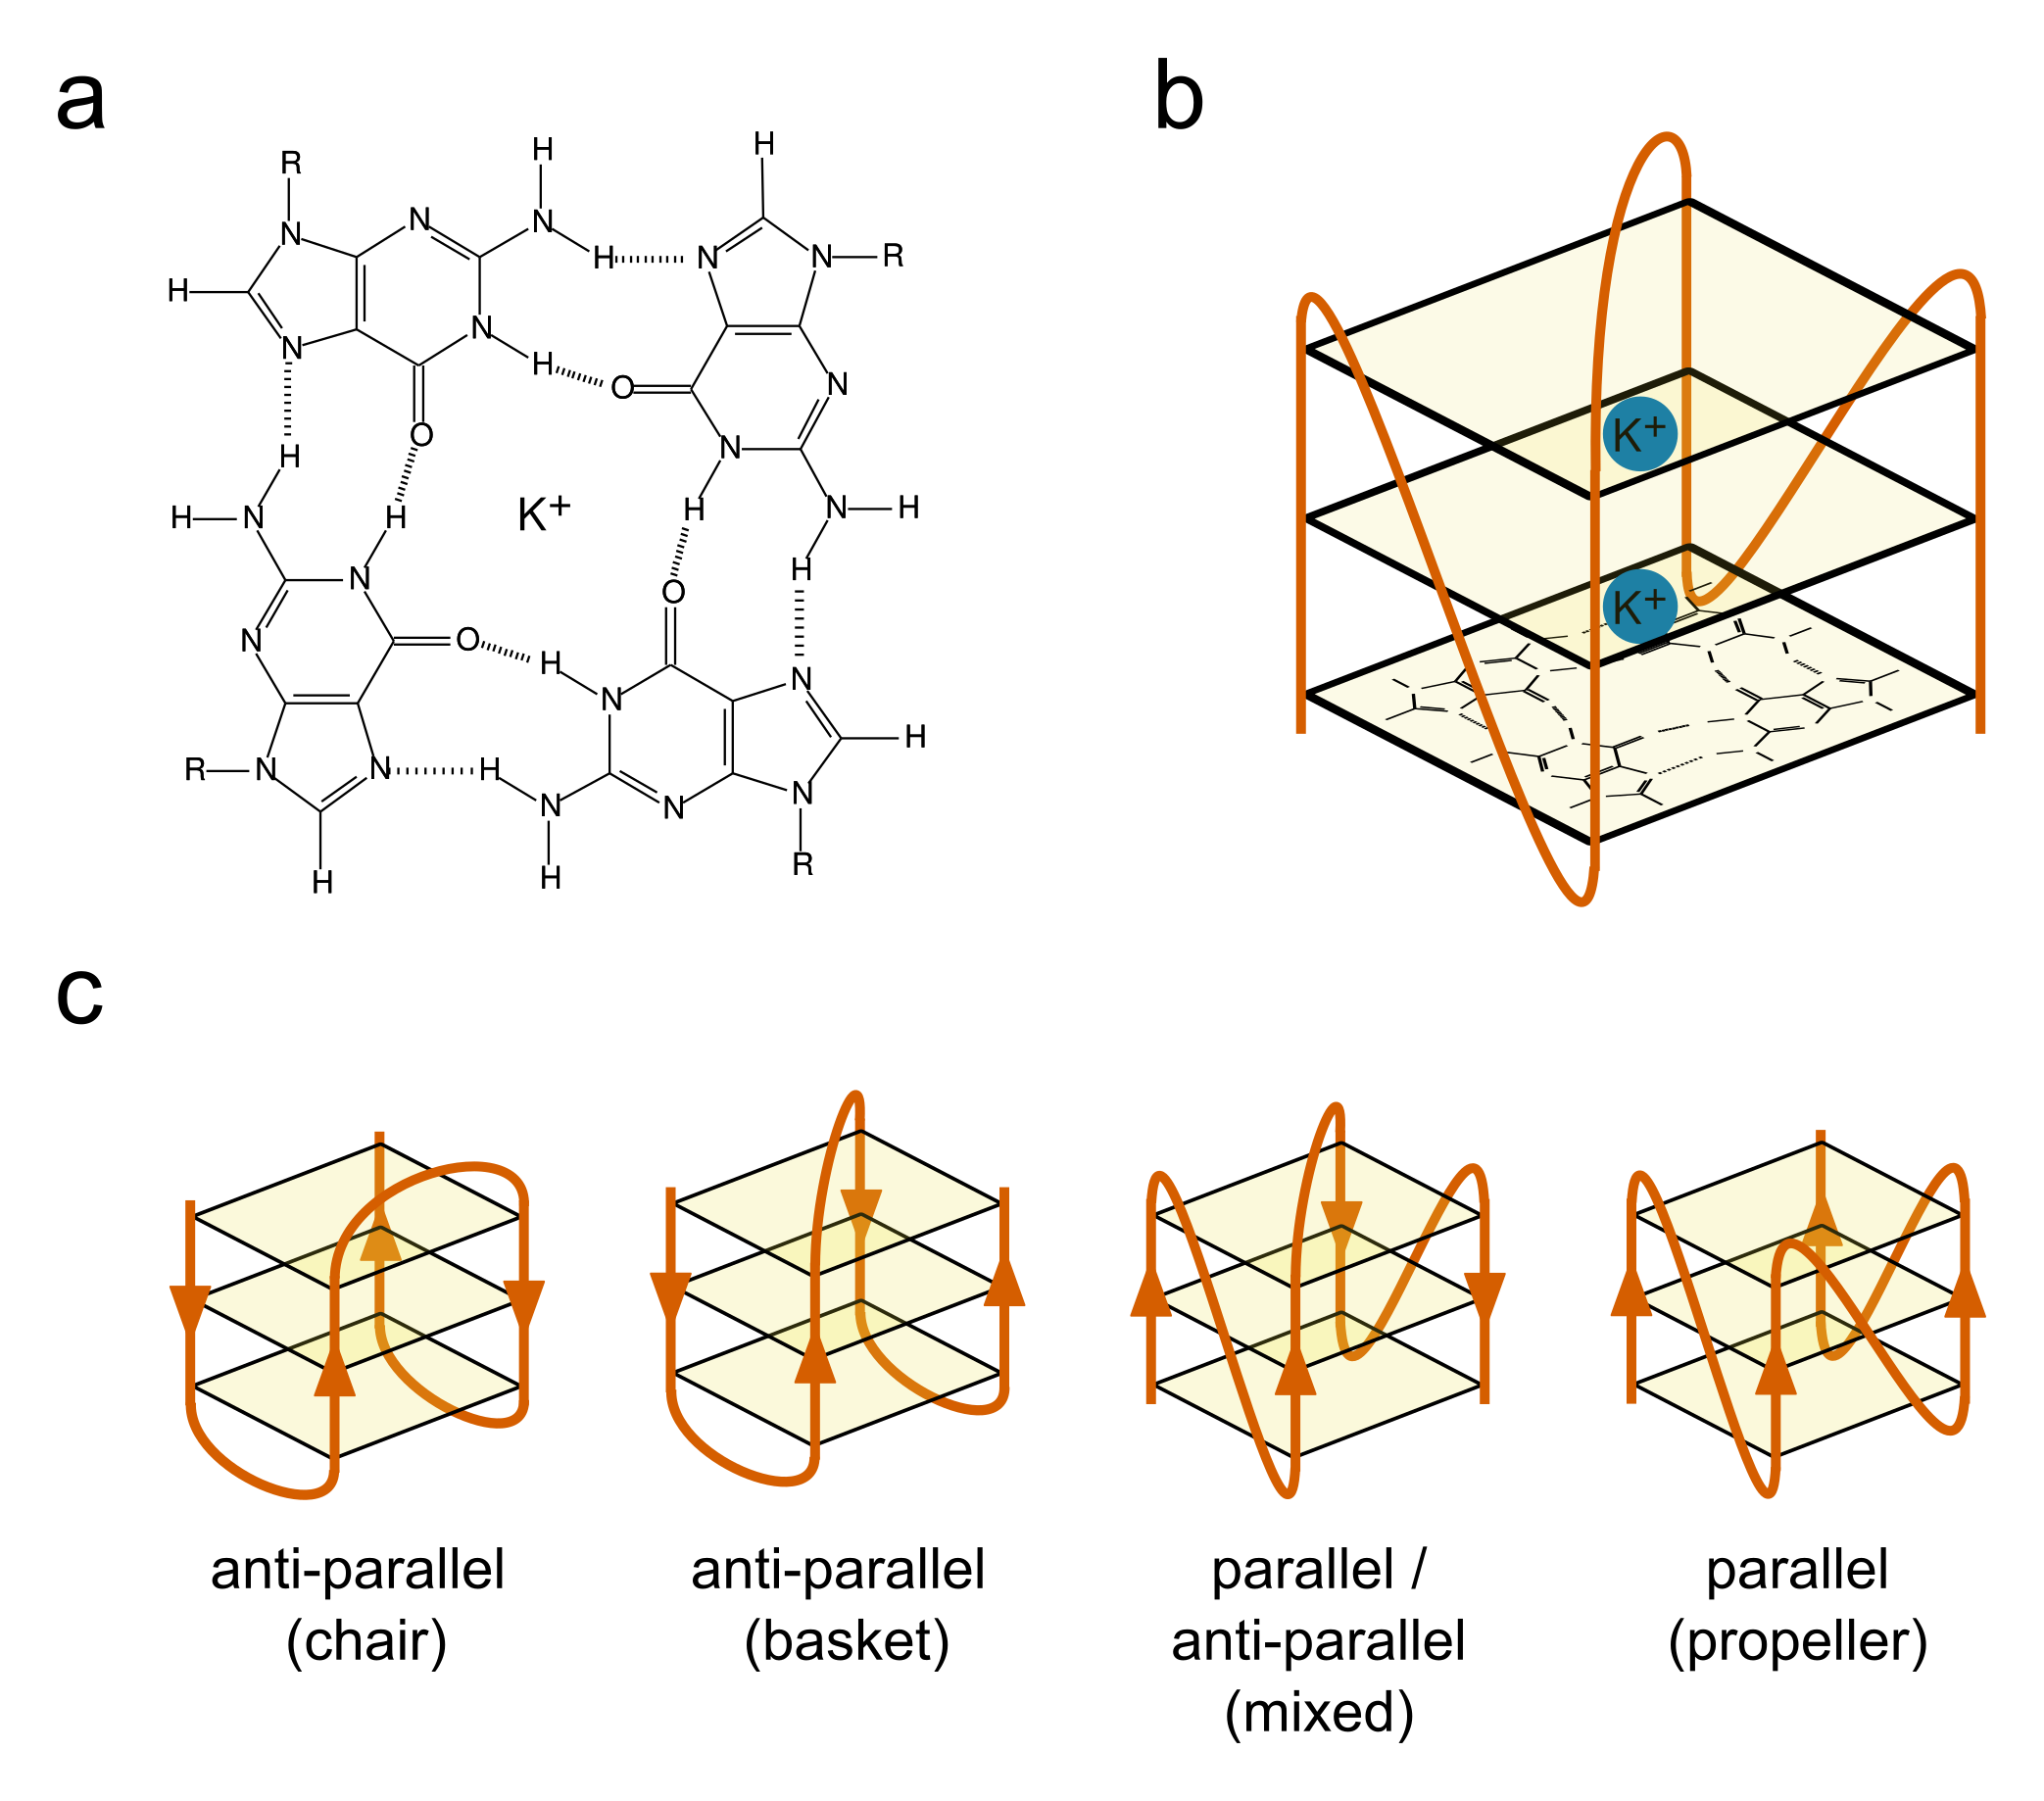
\includegraphics[width=\textwidth,height=562pt,keepaspectratio]{introduction/figures/g4_structure.png}
\caption[Structure of a G-Quadruplex]{\textbf{Structure   of   a   G-Quadruplex}   \textbf{a)}   The   molecular   structure   of   a   G-quartet.   Four   Guanosines   (only   guanine   base   is   shown,   sugar-phosphate   is   represented   as   R)   interact   through   Hoogsteen   base   pairing   around   a   central   monovalent   cation.   \textbf{b)}   Cartoon   showing   the   basic   structure   of   a   three   tetrad   G4.   Three   G-quartets   are   stacked   through   interactions   between   delocalised   pi   electrons.   The   structure   is   made   up   of   four   pillars   of   homopolymeric   G-runs   (shown   in   orange)   joined   by   loop   sequences.   Potassium   cations   (shown   in   blue)   sit   between   each   tetrad.   \textbf{c)}   Cartoons   showing   how   loop   arrangement   can   contribute   to   the   structural   polymorphism   of   G4s.   Loops   can   be   lateral,   diagonal   or   propeller   like,   resulting   in   anti-parallel,   anti-parallel,   and   parallel   G4s   respectively.   Anti-parallel   G4s   with   all   lateral   loops   are   referred   to   as   " chair -like,   whilst   anti-parallel   G4s   with   a   diagonal   loop   are   referred   to   as   basket   like.   G4s   can   also   contain   a   mix   of   parallel   and   anti-parallel   strands.   \label{g4_struct}}
\end{figure}

\newpage

\begin{figure}[htbp]
\centering
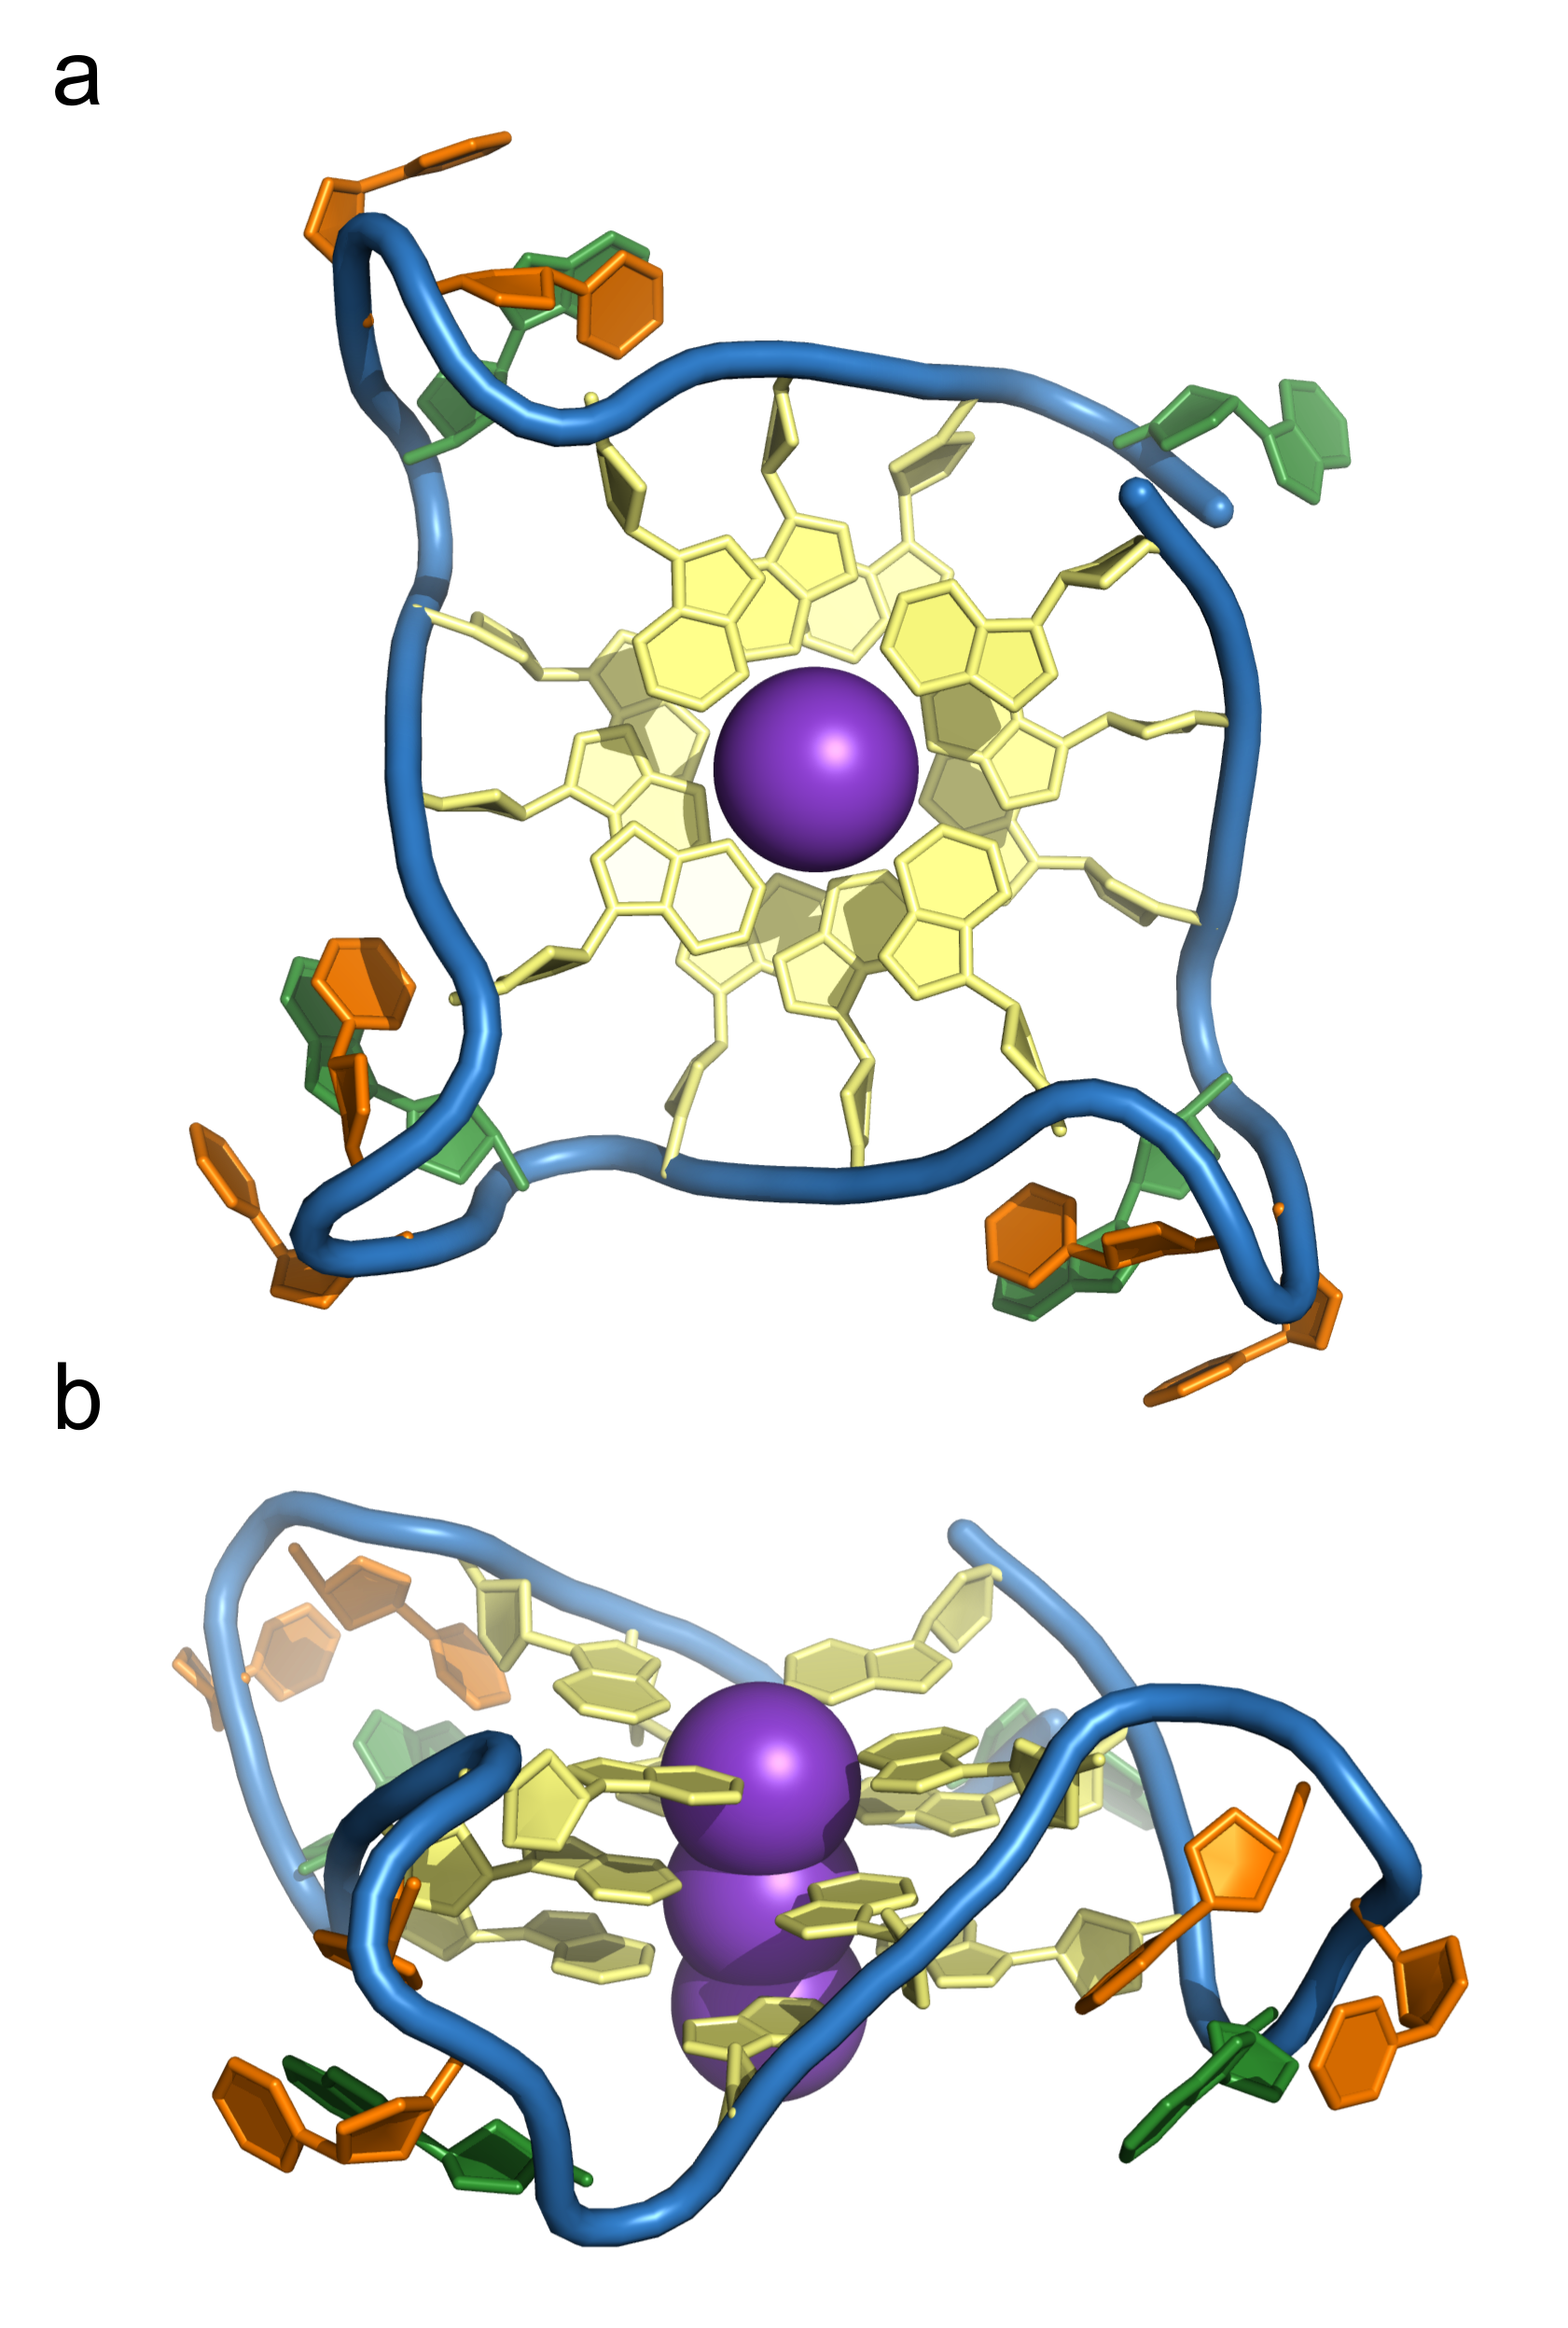
\includegraphics[width=\textwidth,height=562pt,keepaspectratio]{introduction/figures/xray_structure.png}
\caption[The Human Telomeric Sequence forms a G-Quadruplex]{\textbf{The   Human   Telomeric   Sequence   forms   a   G-Quadruplex}   \textbf{a)}   top   and   \textbf{b)}   side   view   of   a   parallel   G4   structure   solved   by   X-ray   crystallography   (PDB:   1KF1,   Parkinson   et   al. 2002).   The   sequence   used   is   (TTAGGG)4,   corresponding   to   four   of   the   human   telomeric   repeat.   Gs   are   coloured   in   yellow,   As   in   green   and   Ts   in   orange.   Potassium   cations   are   coloured   in   purple.}
\end{figure}

\newpage

\hypertarget{g-quadruplex-prediction-from-sequence}{%
\subsection{G-Quadruplex Prediction from
Sequence}\label{g-quadruplex-prediction-from-sequence}}

\label{ssec:predict_g4s}

Genomic G4s form in sequences with high GC content; i.e.~high ratio of
G:C to A:T base pairs, and high GC skew; i.e.~high ratio of G to C on
one strand of the DNA. Because of the dependence of G4 structure on
sequence, it is theoretically possible to computationally predict the
genome-wide prevalence of G4s from sequence information alone, assuming
that other conditions such as potassium concentration are held constant.
The first attempt to characterise putative G4s (PG4s) at whole genome
scale was conducted by Huppert and Balasubramanian in 2005. They
formulated rules describing the general patterns that PG4 forming
sequences tend to follow. Their first observation was that
intermolecular G4s are unlikely to be common \emph{in vivo} due to low
strand concentration of the DNA. They also noted that the pillars of the
G4 tended to be formed from contiguous guanine homopolymers, or G-runs:
there have to be four such G-runs in close proximity to create a PG4.
The length of the shortest G-run will determine the maximum number of
stacked tetrads which can be formed. A minimum of three tetrads was
suggested for prediction: whilst 2 tetrad G4s are possible, they are
less stable. Finally, they suggested that to make folding of the G4
favourable, the length of the loop sequences connecting the G-runs
should be relatively short. They suggested, using evidence from
molecular modelling and CD spectroscopy, an upper limit of 7bp. Again,
whilst loops of much longer length are possible (Guédin et al., 2010),
they were thought likely to be unstable. Their observations were
combined to create the folding pattern
\(G_XN_{1-7}G_XN_{1-7}G_XN_{1-7}G_X\), where \(X \geq 3\). This was
named the Quadparser method (Huppert and Balasubramanian, 2005), and can
be applied to search genomes using simple regular expression machinery.

The Quadparser method has been successfully used to identify G4s in many
organisms, however the it is not perfect and results in many false
negatives as well as false positives. Various adjustments can and have
be made to the pattern, including increasing loop length to a maximum of
12bp, allowing two tetrad PG4s, and allowing short bulges in G-runs
(Chambers et al., 2015). Several tools have been released which attempt
to include these sequences amongst matches (Varizhuk et al., 2014;
Dhapola and Chowdhury, 2016; Hon et al., 2017). These tend to increase
the recall of the method but can also greatly increase the number of
false positives. Other methods have been proposed, such as G4Hunter
(Bedrat et al., 2016), which allow PG4s to be given a numeric score
based on the GC content and skew of the sequence. G4Hunter is generally
performed using a sliding window between 20 and 40bp in length, and is
evaluated for each window by the following method:

\begin{Shaded}
\begin{Highlighting}[]
\NormalTok{score }\OperatorTok{=} \DecValTok{0}
\ControlFlowTok{for}\NormalTok{ base, run_length }\KeywordTok{in}\NormalTok{ run_length_encode(sequence):}
    \ControlFlowTok{if}\NormalTok{ base }\OperatorTok{==} \StringTok{'G'}\NormalTok{:}
\NormalTok{        score }\OperatorTok{+=} \BuiltInTok{min}\NormalTok{(run_length, }\DecValTok{4}\NormalTok{) }\OperatorTok{**} \DecValTok{2}
    \ControlFlowTok{elif}\NormalTok{ base }\OperatorTok{==} \StringTok{'C'}\NormalTok{:}
\NormalTok{        score }\OperatorTok{-=} \BuiltInTok{min}\NormalTok{(run_length, }\DecValTok{4}\NormalTok{) }\OperatorTok{**} \DecValTok{2}
    \ControlFlowTok{else}\NormalTok{:}
        \ControlFlowTok{pass}
\NormalTok{score }\OperatorTok{/=} \BuiltInTok{len}\NormalTok{(sequence)}
\end{Highlighting}
\end{Shaded}

Sequences which have high PG4 forming ability on the positive strand
will therefore be given strong positive scores, whilst sequences with
PG4 forming ability on the negative strand will be given strong negative
scores. A threshold value is chosen below which to filter out non-PG4
forming sequences. Bedrat et al argued that this method was an
improvement over the Quadparser technique because it was more flexible,
however it also results in a much greater number of false positives when
applied to a whole genome, since there are no constraints on how the
G-runs are arranged in the windowed sequence. These methods will be
discussed further in \autoref{chap:g4seeqer}.

\newpage

\hypertarget{methods-used-in-the-characterisation-of-g-quadruplexes}{%
\subsection{Methods used in the characterisation of
G-Quadruplexes}\label{methods-used-in-the-characterisation-of-g-quadruplexes}}

\label{ssec:biophys_char_g4s}

Gellert et al.~first characterised G4 structure using X-ray diffraction
of fibres from dehydrated guanine gels (Gellert et al., 1962). Since
then, biophysical techniques have become key in the study of G4
structures \emph{in vitro}. Since the advent of chemical DNA
oligonucleotide synthesis in the 1980s, it has become relatively cheap
to order high purity single stranded oligonucleotides for PG4 sequences,
and produce micromolar concentration solutions which can be probed by
EMSA, DMS footprinting, FRET, CD spectroscopy or NMR.

Circular dichroism (CD) spectroscopy utilises the difference in
absorbance of circularly polarised light by molecules with chiral
structures (i.e.~with non-superimposable mirror images). Parallel and
anti-parallel G4s both exhibit unique CD absorbance spectra which are
distinct from the spectra of disordered single stranded DNA
(Villar-Guerra et al., 2017). Solutions containing multiple
subpopulations of different parallel and antiparallel G4s will produce
spectra which are more complex to interpret, but are still clearly
distinct from unordered DNA. Melting temperatures of G4s can be
determined using CD or UV spectroscopy temperature gradients measured at
295nm (Villar-Guerra et al., 2017).

Nuclear magnetic resonance spectroscopy (NMR), specifically
Proton-exchange spectroscopy (1H-NMR), can also be used to identify G4
DNA (Silva, 2007). NMR is conducted in deuterated water, since deuterium
has a spin of 1 and therefore does not contributed to the NMR spectrum.
In single or double stranded DNA, imino protons in the guanine
nucleotides will be exchanged with the solvent on short timescales,
resulting in loss of the imino proton signal as they are replaced with
deuterated protons. In G4 DNA, on the other hand, imino protons are
located centrally within the G4 structure, and are therefore protected
from exchange. This means that the 1H spectra can be used to distinguish
G4s from unordered ssDNA. It does not, however, identify whether the G4
has parallel or anti-parallel topology. Further characterisation can be
conducted using Nuclear Overhauser effect spectroscopy (NOESY) to
identify spatial relationships between protons in the G4 (Silva, 2007).

Finally, since folded G4s with short loops and flanking sequence are
relatively globular, a number of G4 structures have been crystallised
from oligomers. The structures of these crystals have then been solved
by X-ray crystallography (Parkinson et al., 2002; Nicoludis et al.,
2012a).

Studies of the structure of G4s has led to the development of a variety
of G4-binding ligands, which might have potential as anti-cancer agents
(Mergny and Helene, 1998; Neidle, 2010; Balasubramanian et al., 2011).
These have a wide range of structures and bind to the various G4
topologies with different strengths (Monchaud and Teulade-Fichou, 2008).
The three major classes of G4 binding ligands are: * \textbf{external
stacking ligands}, which have delocalised pi electron systems, and stack
on the the hydrophobic surfaces of the outer G4 tetrads; *
\textbf{intercalating ligands} , which bind in the groove between
stacked tetrads; * \textbf{external groove binding ligands}, which
insert into the groove of the G4 helix, or interact with loop sequences
(Monchaud and Teulade-Fichou, 2008).

Small molecules which bind G4s include: - \textbf{N-methyl-mesoporphyrin
(NMM)}, an external stacking porphyrin ligand (Nicoludis et al., 2012a);
TMPyP4, another porphyrin derived ligand with multiple binding modes
including external stacking and intercalation (Haq et al., 1999; Phan et
al., 2005) (Fig \ref{drugs}a). NMM is known to prefer parallel G4s
(Nicoludis et al., 2012a); - \textbf{TMPyP4}, a porphyrin derived ligand
with multiple binding modes including external stacking and
intercalation (Haq et al., 1999; Phan et al., 2005). Externally stacked
TMPyP4 has been reported to prefer parallel G4s over anti-parallel
(Arora and Maiti, 2008; Nagesh et al., 2010); - \textbf{Pyridostatin},
an external stacking molecule specifically designed for G4 binding
(Rodriguez et al., 2008) (Fig \ref{drugs}b). Pyridostatin is thought to
bind to all G4s equally well (Müller et al., 2010); -
\textbf{Berberine}, a naturally occurring alkaloid and G4 external
stacking agent (Fig \ref{drugs}c) (Wu et al., 1999; Franceschin et al.,
2006). Berberine has been reported to bind to both parallel and
anti-parallel G4s (Bazzicalupi et al., 2013; Li et al., 2017).

These molecules have been used to study G4s \emph{in vitro} and also
\emph{in vivo}. G4 binding ligands have been shown to have different
binding affinities for G4s derived from different sequences, hinting at
the potential of drugs targeting G4s in specific gene promoters (Weldon
et al., 2018).

\newpage

\begin{figure}[htbp]
\centering
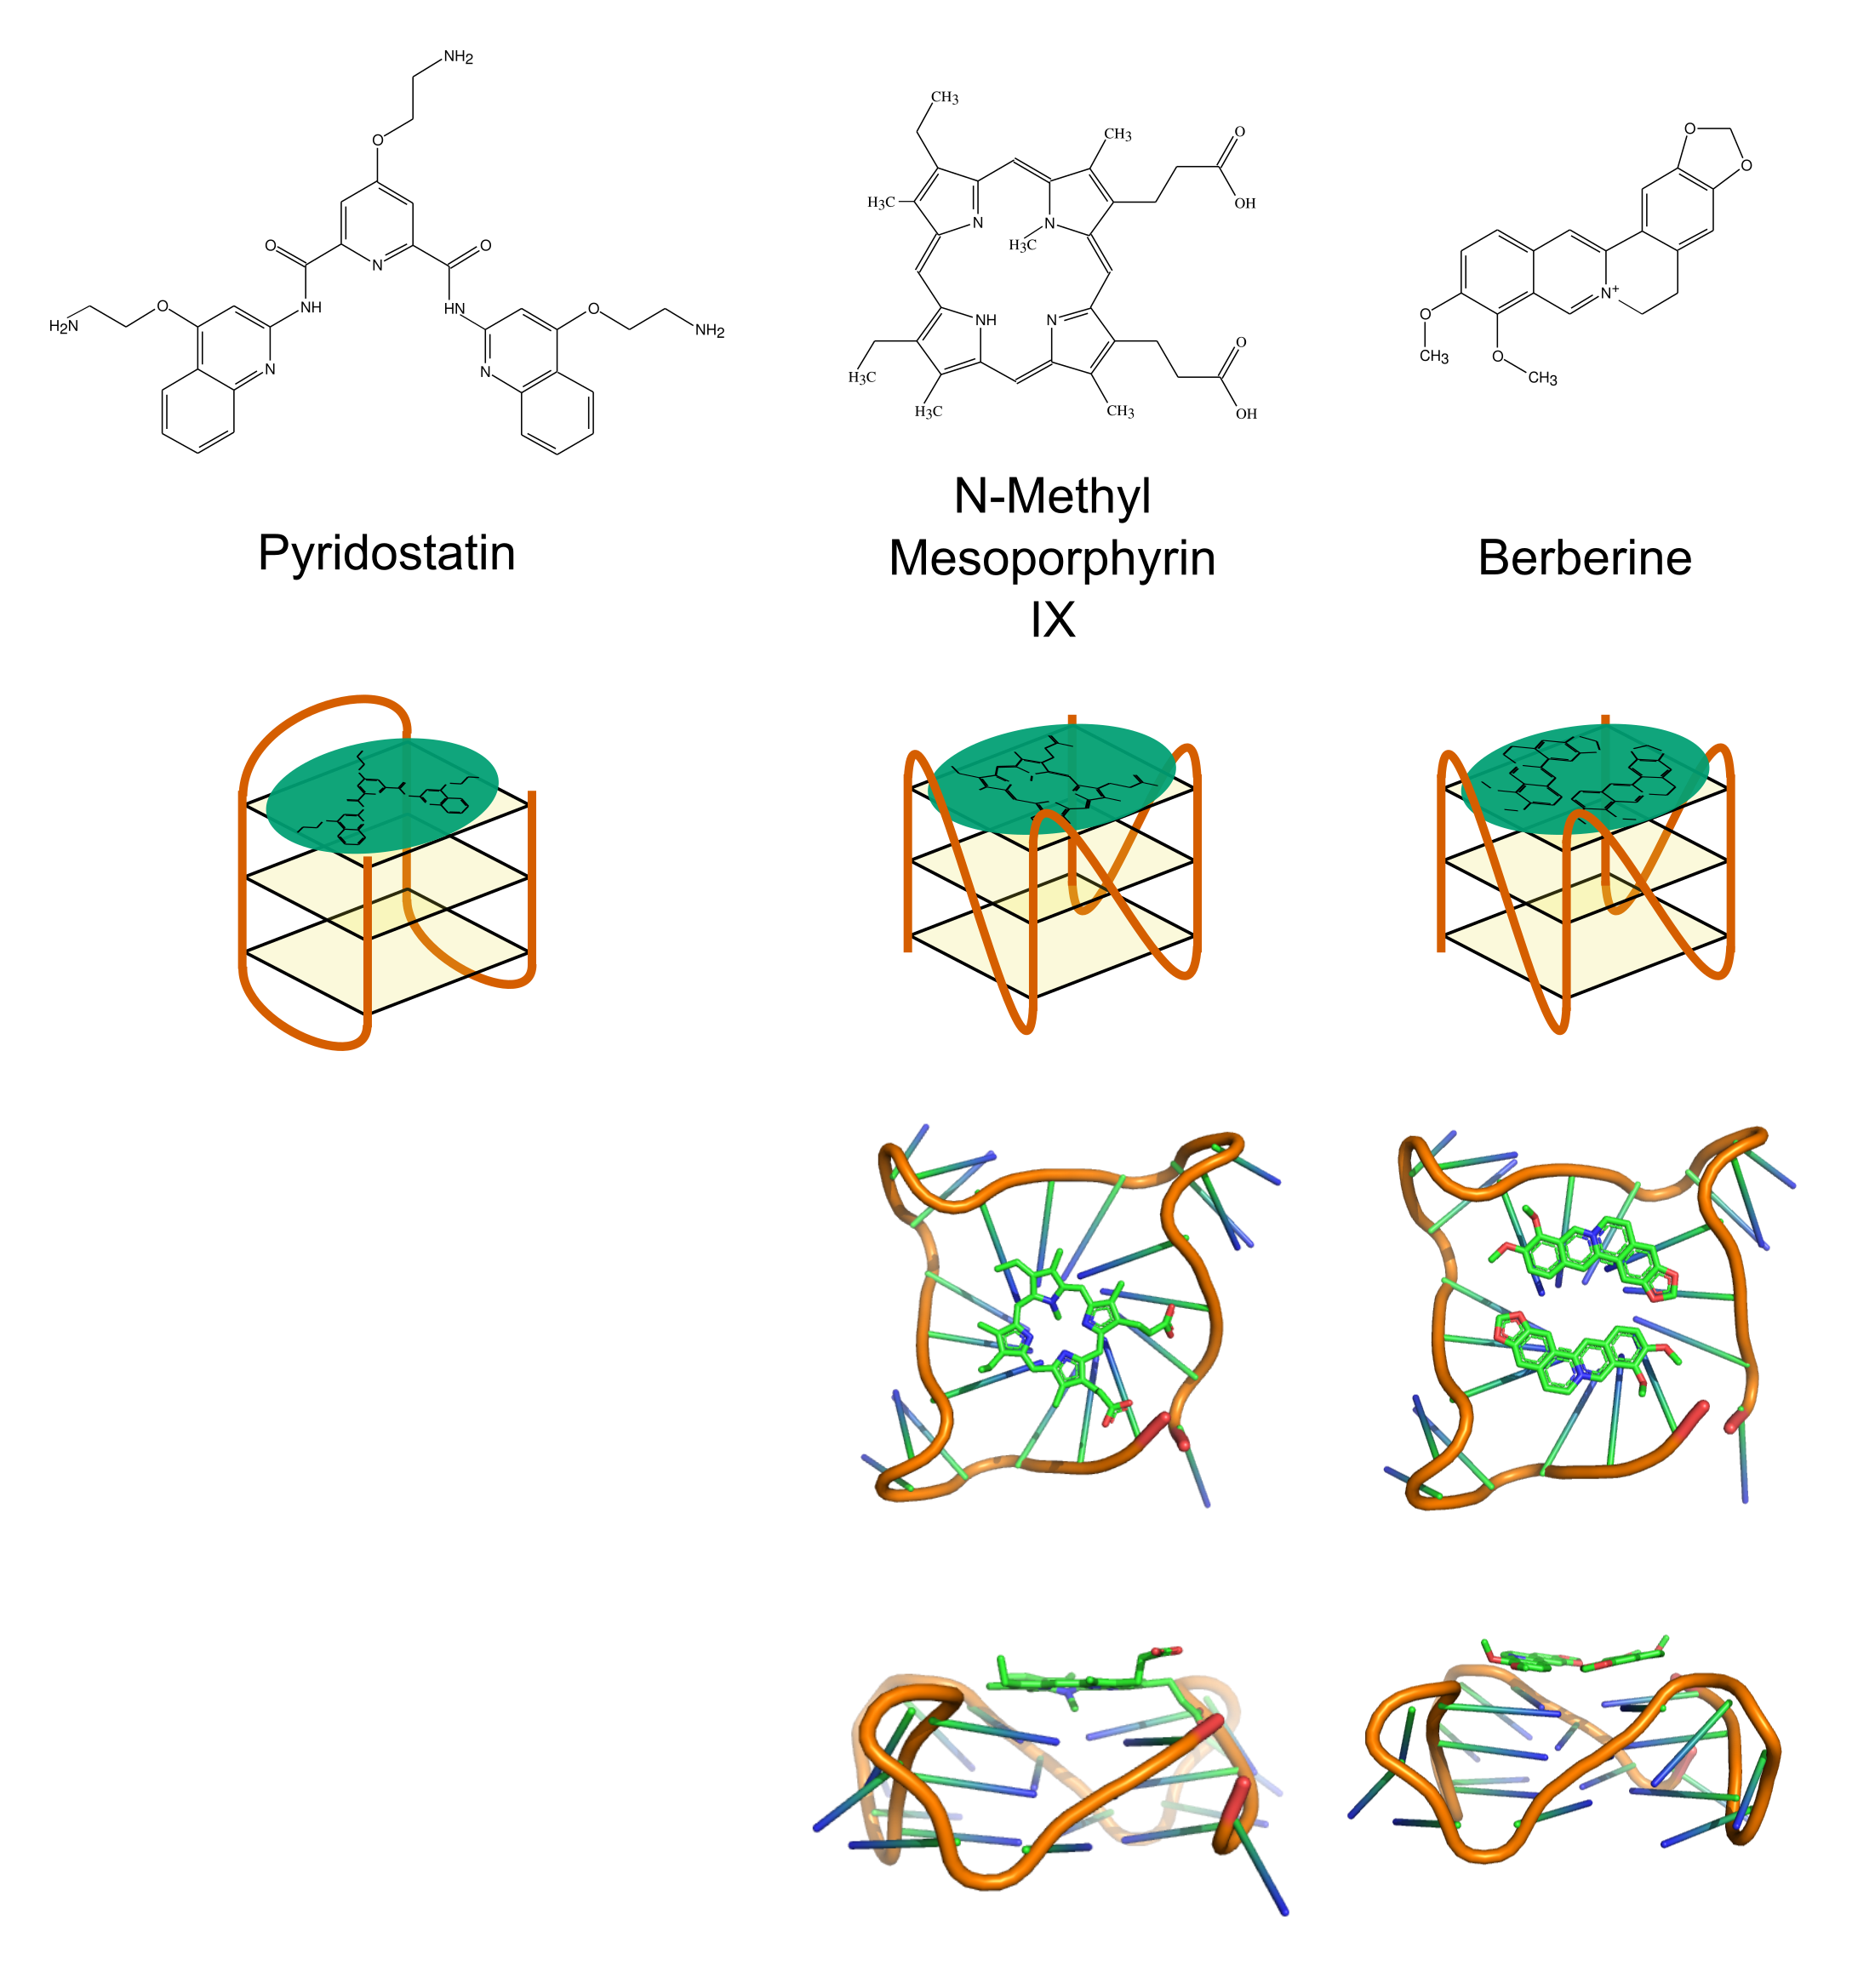
\includegraphics[width=\textwidth,height=562pt,keepaspectratio]{introduction/figures/drugs.png}
\caption[G-Quadruplex Stabilising Ligands]{\textbf{G-Quadruplex   Stabilising   Ligands}   Structures   and   mode   of   action   of   Pyridostatin   (a),   NMM   (b),   and   Berberine(c).   Crystal   structures   of   human   telomeric   DNA   (parallel   G4   form)   in   complex   with   NMM   and   Berberine   are   from   PDB   entries   4FXM   and   3R6R   respectively   (Nicoludis   et   al. 2012,   Bazzicalupi   et   al. 2013).   Potassium   ions   and   solvent   molecules   have   been   hidden   for   visualisation   purposes.   \label{drugs}}
\end{figure}

\newpage

Whilst biophysical methods have led to a wealth of data on G4 formation
\emph{in vitro}, biological evidence of G4 formation has been a much
later development. One common approach to identify cellular G4s, and
study their biological implications, is to treat cells or organisms with
G4 binding ligands such as NMM or Pyridostatin (Hershman et al., 2008;
Nakagawa et al., 2012; Rodriguez et al., 2012). This has been shown to
have various effects on replication, genome stability, transcription and
development {[}REFs?{]}. Naturally fluorescent or fluorophore labelled
small molecules are commonly used to localise G4s by microscopy, or
study their \emph{in vitro} folding by single molecule Förster resonance
energy transfer (smFRET) (Maleki et al., 2017, @Hou2017). Biotinylated
pyridostatin has also been used to pull down G4 DNA structures from
human DNA (Müller et al., 2010).

Moving beyond small molecules, Biffi et al developed an antibody using
synthetic phage display technology that specifically recognises G4 DNA
(Biffi et al., 2013). They used the antibody, named BG4, in
immunofluorescence experiments to visualise G4s in human chromatin
(Biffi et al., 2013). More recently, it was used in Chromatin
Immunoprecipitation sequencing (ChIP-seq) experiments to identify the
specific regions of human chromatin where folded G4s occur
(Hänsel-Hertsch et al., 2016). The biological findings of these
experiments will be discussed in \autoref{sec:biological_roles}.

A number of techniques have been employed for whole genome or
transcriptome mapping of G4s. In a method they named G4-seq, Chambers et
al.~introduced potassium or pyridostatin into the buffer of Illumina
sequencing-by-synthesis reactions (Chambers et al., 2015). This resulted
in G4 formation in the single stranded DNA fragments, which caused
stalling of DNA polymerase, resulting in sequencing errors. They
conducted experiments using this method on single stranded DNA derived
from the human genome. Clusters of identical reads generated by bridge
amplification in an Illumina flow cell were first sequenced normally
(Metzker, 2010). The products of the first sequencing-by-synthesis
reaction were then washed off, and the clusters were resequenced in the
presence of the G4 binding agents. This yielded an initial high quality,
mappable read, and an error prone read. When they mapped the initial
reads to the genome, the number of sequencing errors in each position
was considered an indicator of the G4 forming potential. The authors
showed using this technique that only 30\% of human genomic sequences
found to form G4s \emph{in vitro} conform to the Quadparser motif
(Chambers et al., 2015). This does not, however, address the question of
whether these motifs form G4s \emph{in vivo}.

Yoshida et al.~also used a similar method to identify G4 clusters in
human genomic DNA, by PCR amplifying sequences in the presence and
absence of the G4 binding ligand telomestatin (Yoshida et al., 2018).
They showed that regions which contained G4s were amplified with lower
efficiency in the presence of telomestatin, due to polymerase stalling
events. This resulted in a quantifiable reduction in the number of reads
mapping to G4 containing regions of the genome in the drug positive
samples, relative to the drug negative samples. The authors identified
clusters of motifs predicted to form multiple G4s were more effective at
stalling polymerase than single G4s (Yoshida et al., 2018).

G4s which form in RNA \emph{in vitro} can also be mapped globally, using
a technique called rG4-seq, developed by Kwok et al.~This method again
utilised stalling at G4s, in the presence of potassium or pyridostatin,
this time by the RNA templated DNA polymerase Reverse transcriptase (RT)
(Kwok et al., 2016). They identified positions in mRNAs where a
reproducible drop in reads occurred in samples where RT mediated DNA
synthesis was conducted in the G4 stabilising conditions, relative to
unstabilised controls. Guo and Bartel elaborated on this technique to
map RNA G4s \emph{in vivo}, by treating cells with dimethyl sulphate
(DMS) prior to \emph{in vitro} RT stalling. DMS can penetrate into
living cells and methylate the N7 position of guanines that are not
involved Hoogsteen base paired structures, i.e.~G4s (Wells et al.,
2000). This methylation prevents the refolding of mRNA into G4s \emph{in
vitro}, thereby abolishing RT stalling compared to untreated mRNAs (Guo
and Bartel, 2016). Guo and Bartel identified that the majority of G4s in
yeast and human mRNAs are maintained in an unfolded state \emph{in vivo}
(Guo and Bartel, 2016). The biological implications of this are
discussed in \autoref{ssec:mrna_stability}.

\hypertarget{g-quadruplex-stability-prediction-using-machine-learning}{%
\subsection{G-Quadruplex stability prediction using Machine
Learning}\label{g-quadruplex-stability-prediction-using-machine-learning}}

\label{ssec:g4_machine_learning}

A growing number of G4 forming oligonucleotide sequences have now been
characterised \emph{in vitro} by various methods, particularly by CD
spectroscopy and UV melting, and the melting temperatures have been
published online. The number of these is now great enough that several
groups have utilised them to train machine learning models to predict G4
forming potential. Machine learning is the application of statistical
techniques to identify patterns in large datasets, and produce rules
which will generalise to new data (Larrañaga et al., 2006). The use of
such statistical models in bioinformatic tools has grown greatly since
the advent of techniques such as high throughput sequencing, as they
produce the large amounts of data required for training such methods
(Larrañaga et al., 2006). The use of machine learning in nucleic acid
motif prediction will be discussed in more detail in
\autoref{chap:g4seeqer}.

Stegle et al.~implemented a Gaussian Process model incorporating
extracted features from Quadparser conforming G4s (Stegle et al., 2009).
These features were the number of tetrads, the length of each of the
three loops, the total loop length, and the frequencies of adenine,
cytosine and guanine in the sequence, as well as the raw sequence
itself. A second kernel which incorporated features about the conditions
the melting temperature was acquired under, i.e.~the concentrations of
potassium, sodium, ammonium, and magnesium ions, was also used in the
model. They trained this model on a set of 260 DNA G4 melting
temperatures which were acquired from a literature search. In a cross
validation experiment using 100 random 50\% hold out splits, the authors
were able to achieve a good level of test set accuracy with an average
of 80\% of predictions within 5 degrees of the true melting temperature
(Stegle et al., 2009). Furthermore, their model was interpretable, and
they were able to identify tetrad number and the length of the central
loop as the most important sequence features in PG4 stability. The
authors employed active learning to identify candidates from human
promoter sequences with high uncertainty in the model, and used CD
spectroscopy to characterise them.

Whilst Stegle et al.'s model was successful on Quadparser conforming
motifs, it is estimated that \textasciitilde{}70\% of G4s in the human
genome do not conform to this motif (Chambers et al., 2015). More
recently, Garant et al.~published a method for predicting RNA G4s which
was trained on a set of 368 experimentally determined sequences, 149 of
which were G4 positive and 179 of which were G4 negative (Garant et al.,
2017). From these sequences the trinucleotide contents were extracted,
and used to train a densely connected multi-layer perceptron model, with
a single hidden layer containing 35 nodes. This trinucleotide trained
model had the advantage being more flexible for G4s that do not conform
to the Quadparser motif. Their model achieved an average AUC score of
0.92 on hold out sets in a 5 fold cross validation experiment. When
tested on the rG4-seq dataset of RT stalled RNA G4s (Kwok et al., 2016),
the method did not perform as well as G4Hunter (Bedrat et al., 2016).
This indicates that some positional information is lost when sequences
are converted to trinucleotide content features.

Finally, the more recent efforts to produce high-throughput methods for
identifying genomic G4s, such as G4-seq developed by Chambers et al.,
have created much better in depth datasets for training machine learning
models. Sahakyan et al.~used the G4-seq dataset in their model. This was
a extreme gradient boosted machine model developed using
\texttt{xgboost} (Chen and Guestrin, 2016), which regressed the
percentage mismatch score of sequences from the G4-seq dataset which
conform to the Quadparser method (Sahakyan et al., 2017). The authors
extracted features from Quadparser conforming PG4s similar to those
employed by Stegle et al., including tetrad number, loop length, and
mono-, di- and triunucleotide contents of the PG4, and flanking regions.
This model was very successful at identifying Quadparser conforming
motifs which did or did not actually form G4s, achieving a root mean
squared error score of 8.14 (units used were mismatch score in G4-seq
experiment, in percentage format) (Sahakyan et al., 2017). The method
could not identify non-Quadparser conforming G4 motifs, however, which
make up a large proportion of experimentally characterised G4s (Chambers
et al., 2015).

\newpage

\hypertarget{other-g-rich-nucleic-acid-structures}{%
\subsection{Other G-rich Nucleic Acid
Structures}\label{other-g-rich-nucleic-acid-structures}}

G4s are not the only DNA or RNA structures which occur specifically in
sequences with high GC content and skew. Another structure is the R
loop, which can form when transcription of a C-rich template strand to a
G-rich RNA molecule occurs (Reaban et al., 1994; Li and Manley, 2005;
Ginno et al., 2012, 2013). This RNA molecule is complementary to the
template strand, and can therefore form a DNA:RNA hybrid duplex, leaving
the coding strand of the DNA in a single stranded form (Skourti-Stathaki
et al., 2014). Once formed, these hybrids are more thermodynamically
stable than normal DNA:DNA duplexes (Roberts and Crothers, 1992). This
could be partially explained to the formation of G4 structures in the
G-rich single stranded DNA of the coding strand (Duquette et al., 2004).
The biological implications of R loop formation and their interactions
with G4 structures are discussed briefly in \autoref{ssec:rloop_csr}.

\newpage

\hypertarget{biological-roles-of-g-quadruplexes}{%
\section{Biological Roles of
G-Quadruplexes}\label{biological-roles-of-g-quadruplexes}}

\label{sec:biological_roles}

\hypertarget{genome-stability-dna-replication}{%
\subsection{Genome Stability \& DNA
Replication}\label{genome-stability-dna-replication}}

\label{ssec:genome_stability}

The distribution of G4s in genomes has been predicted from sequence for
a wide variety of organisms (Huppert and Balasubramanian, 2005; Du et
al., 2008; Hershman et al., 2008; Mullen et al., 2010; Garg et al.,
2016), and has been experimentally determined by the techniques
mentioned above for the human genome. There is conclusive evidence that
G4s are not uniformly distributed throughout genomes, but tend to be
clustered at functional locations. By far the strongest enrichment of
G4s is seen at telomeres. G4s are also found more than would be expected
in origins of replication, gene promoters, and inside gene bodies,
particularly the 5' and 3' untranslated regions (UTRs). In these
locations, it has been demonstrated that G4 formation has effects on the
processes of DNA replication, genome stability, transcription, and
translation.

Perhaps the best characterised biological role for is at the telomeres.
Telomeres are the protein-DNA structures found at the ends of linear
eukaryotic chromosomes. They consist of thousands of tandem repeats of a
G-rich sequence (Moyzis et al., 1988), with a single stranded overhang
of around 100-200bp (Makarov et al., 1997). Due to functional
limitations in templated DNA replication, the very ends of these cannot
be duplicated during cell division. This means that without
intervention, the chromosome will gradually shorten with each division.
Telomeres therefore serve as protective caps that prevent the loss of
important coding DNA from the genome. In humans, the telomeric repeat is
(TTAGGG)n (Moyzis et al., 1988). This has been identified through
various methods as a G4 forming sequence.

Telomeres are coated in architectural proteins, called telomere end
binding proteins (TEBPs), which protect the DNA from recognition by DNA
damage response pathways. Giraldo \& Rhodes showed that a yeast TEBP,
RAP1, induces formation of G4 structures in telomeres \emph{in vitro}
(Giraldo and Rhodes, 1994). More recently, immunofluorescence
experiments using the BG4 antibody showed that G4 foci overlap with
fluorescent foci produced by Fluorescent \emph{In Situ} Hybridisation
(FISH) of the telomeric repeat in human HEK 293T cells (Moye et al.,
2015). These results suggest that telomeric sequences do form G4s
\emph{in vivo}, which may be bound and stabilised by TEBPs. Furthermore,
Moye et al.~identified that telomerase, the template-independent DNA
polymerase which synthesises new telomeric repeats, is able to bind to
and partially unwind parallel G4s, but not anti-parallel G4s (Moye et
al., 2015). There is therefore the suggestion of a G4 regulated
mechanism for telomere maintenance.

G4s seem to also play roles in other aspects of DNA replication. It is
well documented that G4s are capable of stalling polymerases \emph{in
vitro}. There is also growing evidence that without the assistance of G4
unwinding helicases, G4s might cause polymerase stalling \emph{in vivo}.
Work by Rodriguez et al.~demonstrated that treatment of human cancer
cells with G4 stabiliser pyridostatin causes an increase in the DNA
damage marker γH2AX, suggesting an increase in double strand breaks
(DSB) (Rodriguez et al., 2012). This damage was ameliorated by treatment
with a DNA replication inhibitor, suggesting the damage was caused
during replication. This is likely to be the result of replication fork
collapse at G4 DNA blockages. The DNA helicase FANCJ, which is a
tumour-suppressor gene often mutated in breast and ovarian cancers, is
involved in DSB repair and has been shown to preferentially bind and
unwind G4s (Wu and Spies, 2016). Mutation of the FANCJ ortholog DOG1 in
\emph{C. elegans} results in genome instability, and accumulation of
deletions upstream of G4s (Kruisselbrink et al., 2008).

The Bloom gene (BLM) encodes a DNA helicase which, when mutated in
humans, causes Bloom's Disease (German, 1993). This is characterised by
a reduction in genome stability resulting from a large increase in
sister chromatid exchange events (SCE). SCEs are caused by double strand
breaks, which are repaired via homologous recombination (Wu, 2007). BLM
has been shown to prevent SCEs by unwinding Holliday Junctions (a common
form of branched duplex), and restarting collapsed replication forks
(Davies et al., 2007). Work by Sun et al.~first showed that BLM is also
capable of binding and resolving G4s \emph{in vitro} (Sun et al., 1998).
Recently, van Wietmarschen et al.~used a single cell sequencing
technique to map the locations of SCEs in cells lacking function BLM,
and found that many SCEs were at sites predicted to form G4s (Van
Wietmarschen and Lansdorp, 2016). This suggests that direct action of
helicases is required to prevent genome instability at G4 loci.

In humans, DNA replication occurs from tens to hundreds of thousands of
origins of replication which are found at regular distances of around
10-100kb apart (Huberman and Riggs, 1968; Besnard et al., 2012). Using
genome-wide mapping of replication origins by short nascent strand
sequencing, Besnard et al.~identified that the majority of human origins
were in GC rich regions of DNA, and that 67\% overlapped with motifs
conforming to the Quadparser pattern (Besnard et al., 2012). 91\% of
origins were associated with G4s with extended loop lengths of up to
15bp. Furthermore, they found an association between the number of G4
motifs, and the strength of usage of origins, suggesting that G4s might
be a recruiting factor for replication machinery.

\newpage

\begin{figure}[htbp]
\centering
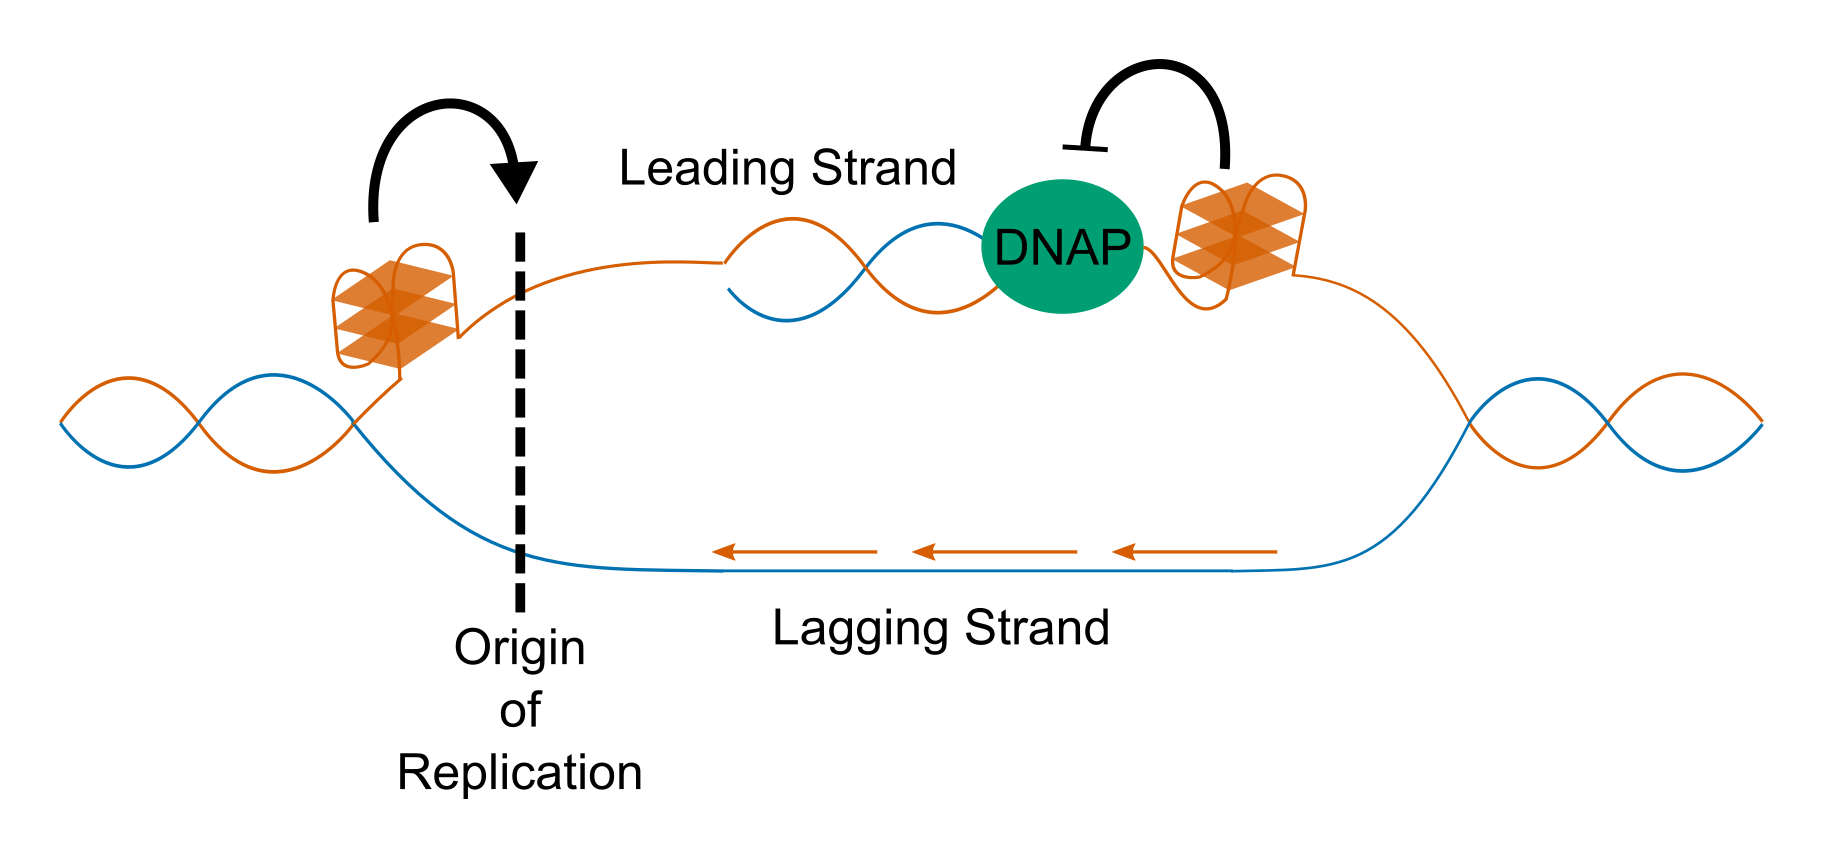
\includegraphics[width=\textwidth,height=562pt,keepaspectratio]{introduction/figures/replication.png}
\caption[Role of G4s in DNA replication]{\textbf{Role   of   G4s   in   DNA   replication}   Illustration   showing   the   possible   mechanisms   of   G4   involvement   in   DNA   replication.   Besnard   et   al. identified   that   a   majority   of   human   replication   origins   contain   a   PG4,   suggesting   that   G4s   may   recruit   replication   machinery   (Besnard   et   al.,   2012).   In   the   absence   of   G4   unwinding   helicase   FANCJ,   Kruisselbrink   et   al. identified   deletions   downstream   of   PG4   loci,   suggesting   G4s   cause   replication   fork   collapse.   \label{replic}}
\end{figure}

\newpage

\hypertarget{transcription}{%
\subsection{Transcription}\label{transcription}}

\label{ssec:transcription}

Transcription is the process by which DNA is copied into messenger RNA
(mRNA) or non-coding RNA (ncRNA), by a DNA-templated RNA polymerase. In
eukaryotic systems, all mRNA is transcribed by RNA Polymerase II (Pol
II). Initiation of transcription is often catalysed by general or
specific transcription factors which bind to the promoter region,
upstream of the transcriptional start site (TSS). Human promoter
sequences are enriched for PG4 motifs conforming to the Quadparser motif
(Eddy and Maizels, 2006; Huppert and Balasubramanian, 2007). Tumour
suppressor genes have fewer promoter PG4s than might be expected by
chance, whilst proto-oncogenes contain more than might be expected (Eddy
and Maizels, 2006). PG4s also overlap with regions of open chromatin,
detected by methods such as DNase Hypersensitivity sequencing
(DNase-seq) or Assay for Transposable-Accessible Chromatin by Sequencing
(ATAC-seq), suggesting they are often actively transcribed (Huppert and
Balasubramanian, 2007). Hänsel-Hertsch et al.~used the BG4 antibody to
perform ChIP-seq of G4 structures in conjunction with ATAC-seq and
RNA-seq, in normal human keratinocytes and an immortalised cell line
(Hänsel-Hertsch et al., 2016). They found that BG4 peaks were indeed
associated with open promoters, and were found upstream of expressed
genes (Hänsel-Hertsch et al., 2016). Interestingly, many more BG4 peaks
were identified in the immortalised cells than in normal cells, despite
having similar levels of open chromatin. Furthermore, genes which only
had a promoter BG4 peak in the immortalised cells tended to be more
highly expressed in those cells compared to the normal cells, suggesting
that promoter G4s may increase gene expression. A potential mechanism
for this increase in expression might be the result of recruitment of
positive transcription factors.

Perhaps the most well-studied promoter G4 is the Nuclease Hypersensitive
Element III (NHEIII) found in the promoter of the c-MYC oncogene. The
NHEIII contains a number of G-rich tracts which have been shown to form
G4s \emph{in vitro} by a variety of methods (Simonsson et al., 1998;
Siddiqui-Jain et al., 2002; Seenisamy et al., 2004; Ambrus et al.,
2005). Formation of a G4 by this region has a strongly repressive effect
on gene expression. Siddiqui-Jain et al.~found that treatment of cells
with the G4 stabilising agent TMPyP4 led to repression of c-MYC, whilst
G4 abolishing mutations in a c-MYC promoter luciferase assay caused a
three-fold increase in expression (Siddiqui-Jain et al., 2002).
Pull-down of NHEIII binding factors by González et al.~identified
Nucleolin as a potential G4 interacting partner (González et al., 2009).
Nucleolin is a multi-functional protein implicated in ribosome
synthesis, transcription and chromatin remodelling. González et al.~went
on to show that Nucleolin binds to the c-MYC promoter \emph{in vivo},
and that nucleolin overexpression results in downregulation of c-MYC
gene expression (González et al., 2009), by promoting G4 formation
(González and Hurley, 2010).

G4s which form within the gene body may have differing effects on
transcription, depending on the strand they occur in. Analysis of human
gene expression data has suggested that genes containing coding strand
G4s downstream of transcriptional start sites tend to have higher
expression at the mRNA level than those that do not (Du et al., 2008),
even when other factors such as gene function are controlled for. It has
been speculated that G4 formation competes with double stranded DNA,
creating single stranded ``bubbles'' which promote Pol II binding and
transcription (Rhodes and Lipps, 2015). Since the coding strand is not
directly used by Pol II, coding strand G4s will not cause polymerase
stalling. G4s which form in the template strand, however, may form
blockages which could slow or pause the progression of Pol II.

Transcription progresses by using the template strand as an antisense
copy to replicate the coding strand sequence in mRNA. G4s which form in
the template strand of gene body DNA will therefore need to be resolved
before Pol II can move through them. Due to the relative stabilities of
dsDNA and G4s, G4 formation may only occur in the gene body after a
pioneering round of transcription, during which the DNA is in single
stranded form (Eddy et al., 2011). Rodriguez et al.~showed that some of
the DNA damage caused by treating cells with pyridostatin was
transcription-dependent, and could be ameliorated by treating cells
additionally with an inhibitor of transcription (Rodriguez et al.,
2012).

\newpage

\begin{figure}[htbp]
\centering
\includegraphics[width=\textwidth,height=562pt,keepaspectratio]{introduction/figures/transcription.png}
\caption[Possible Mechanisms for DNA and RNA G4 function in transcription and gene expression]{\textbf{Possible   Mechanisms   for   DNA   and   RNA   G4   function   in   transcription   and   gene   expression}   \textbf{a)}   Possible   mechanism   for   function   of   G4s   located   in   the   coding   strand.   Since   G4s   form   from   single   stranded   DNA,   G4s   in   the   coding   strand   may   promote   melting   of   double   stranded   DNA,   increasing   transcription   levels.   G4s   which   form   in   the   coding   strand   of   the   exonic   DNA   of   a   gene   will   also   be   present   in   the   mRNA   produced   from   that   locus,   and   G4s   which   form   in   the   coding   strand   of   introns   will   be   present   in   pre-mRNA.   These   RNA   G4s   might   also   influence   gene   expression   through   alteration   of   pre-mRNA   splicing,   mRNA   stability,   or   translation.   \textbf{b)}   Possible   mechanism   for   the   function   of   G4s   located   in   the   template   strand.   The   template   strand   of   genes   is   scanned   by   RNA   Polymerase   II   during   transcription,   and   G4s   which   form   in   ahead   of   the   transcription   complex   may   cause   slowing   or   stalling   if   they   cannot   be   correctly   resolved.   RNA   Polymerase   II   translocation   speed   is   linked   to   a   number   of   co-transcriptional   processes,   including   splicing.   Adapted   from   Figure   4.   Rhodes   and   Lipps,   2015.   \label{mech}}
\end{figure}

\newpage

Methods for estimating Pol II elongation rates across genes, such as
GRO-seq or BruDRB-seq, have associated changes in speed with various
features such as specific histone modifications, exon density, and
sequence features. Veloso et al.~correlated elongation rates from
BruDRB-seq data with GC content of genes, and found that genes with
higher GC content tended to have slower elongation (Veloso et al.,
2014). They hypothesised that this could be due to the greater stability
of GC-rich duplexes, which have extra hydrogen bonds. It is also
possible, however, that this effect could be partially due to greater
numbers of G4s in GC-rich genes.

In human cells, profiling of Pol II occupancy by ChIP-seq has
demonstrated that there is a large peak of paused polymerase in the
first 30-60bp downstream of the TSS (Jonkers and Lis, 2015). This
pausing is an important checkpoint ensuring Pol II is correctly modified
before elongation begins. Genes which require large and rapid increases
in expression in response to environmental stresses, such as heat shock
proteins, also have large amounts of paused Pol II which can be
activated quickly. During initiation of transcription, Pol II is
recruited to the TSS by specific or general transcription factors, and
transcribes for a short distance before becoming paused. Formation of
paused Pol II, referred to as the Pre-Initiation Complex (PIC), is
stabilised by the Negative elongation factor (NELF) and
DRB-sensitivity-inducing factor (DSIF), as well as by phosphorylation of
the carboxy-terminal domain (CTD) of Pol II at Serine 5. Productive
elongation can then be restarted by the action of the positive
transcription elongation factor-b (P-TEFb) complex, which phosphorylates
NELF and DSIF, causing the former to be released from the PIC, and the
latter to switch to becoming a positive elongation factor. P-TEFb also
phosphorylates the CTD at Serine 2, which is considered a hallmark
modification of active Pol II. How Pol II pausing is regulated is still
not clear (Jonkers and Lis, 2015; Liu et al., 2015). One hypothesis is
that the sequence content of promoters and promoter proximal regions may
be important for regulating pausing. A number of promoter motifs, such
as the GAGA motif or the downstream promoter element (DPE) have been
associated with promoters with high levels of stalling (Hendrix et al.,
2008).

It is well established that the promoter proximal regions of genes in
many organisms have, on average, higher GC content than the rest of the
gene body (Veloso et al., 2014). Eddy et al.~identified that the first
200bp downstream of the TSS tends to be more GC-rich in genes with high
levels of proximal pausing than in genes which do not exhibit pausing
(Eddy et al., 2011). The G4-forming potential of these genes also tended
to be greater on the coding strand, meaning that G4 structures might
also form in the nascent mRNA. Eddy et al.~hypothesised that these 5'
mRNA G4s might signal back to the polymerase to produce pausing. A
similar mechanism involving an RNA hairpin has been implicated in
pausing of \emph{E coli} RNA Polymerase (Toulokhonov et al., 2007).

The enrichment of G4s in promoters and promoter proximal regions
suggests that proteins involved in transcriptional complexes may bind
specifically to these structures. The general transcription initiation
factor complex, TFIIH, contains 11 subunits, and is required for both
transcriptional processes and DNA repair through the Nucleotide Excision
Repair (NER) pathway (Compe and Egly, 2016). The DNA helicases XPB and
XPD are essential components of TFIIH, which catalyse the denaturation
of DNA in promoters or around lesions (Coin et al., 2007). Through
\emph{in vitro} binding assays, Gray et al.~identified XPB and XPD as G4
interacting proteins, which bind G4s preferentially over dsDNA (Gray et
al., 2014). XPD was also found to unwind G4s \emph{in vitro}. Gray et
al.~went on to perform ChIP-seq of XPD and XPB, and showed that it was
enriched at TSS loci containing G4s. Approximately 40\% of XPD/XPB peaks
contained PG4s conforming to the Quadparser pattern (with loop lengths
\textgreater{}= 12bp). Furthermore, Hänsel-Hertsch et al.~also reported
a strong overlap between these XPD/XPB peaks and G4 loci observed by BG4
ChIP-seq (Hänsel-Hertsch et al., 2016). This suggests that TFIIH may be
recruited to G4 containing promoters to initiate transcription.

\newpage

\hypertarget{mrna-processing}{%
\subsection{mRNA Processing}\label{mrna-processing}}

\label{ssec:mrna_processing}

Nascent pre-mRNA which is newly transcribed by Pol II must undergo 5'
capping, splicing, RNA modification, poly-adenylation and quality
control before it can mature into mRNA which is exported to the
cytoplasm. Many of these processes occur co-transcriptionally and are
tightly co-ordinated to prevent mistakes. Multiple independent studies
in different organisms estimate that between 75\%-85\% of splicing is
conducted in a cotranscriptional manner (Carrillo Oesterreich et al.,
2010; Ameur et al., 2011; Khodor et al., 2011; Girard et al., 2012;
Tilgner et al., 2012; Windhager et al., 2012). Oesterreich et al.~found
that in yeast, 10\% of intron splicing is complete when Pol II is only
26bp downstream of the intron acceptor site, and 50\% complete when Pol
II is 45bp downstream. (Carrillo Oesterreich et al., 2016). By modifying
Pol II to increase its speed 2.3x, they also showed that splicing could
become rate limiting when elongation rate is greater. Furthermore,
modifications to splice site sequences in a reporter reduced the rate of
splicing, presumably by reducing the strength of recognition by snRNAs,
and thereby the rate of spliceosome assembly (Carrillo Oesterreich et
al., 2016). This indicates that interplay of splice site strength and
Pol II elongation speed determine the relative efficiency of splicing.

It has been estimated that greater than 90\% of human genes undergo some
form of alternative splicing (Wang et al., 2008). During this process,
different donor and acceptor sites compete to be utilised. The most
common form of alternative splicing in humans is exon skipping, where
constitutive donor and acceptor sites are paired such that an
intervening exon is removed from the mature mRNA (Kim et al., 2007).
Other forms include alternate donor or acceptor usage, where the other
site used is constitutive, or intron retention, where splice sites are
simply not used at all (Wang et al., 2014). Regulation of alternative
splicing can occur via protein splicing factors, as well as through
changes in Pol II elongation speed (Mata et al., 2010; Jonkers and Lis,
2015). Through this mechanism, alternative splicing may be linked to
changes in Pol II speed as it transcribes through template stranded G4s
or other DNA structures.

Aside from their effects on Pol II speed, G-rich sequences with the
potential to form G4s have been implicated as important intron motifs
for splicing. These PG4s are predicted in the coding strand, meaning
that they could form G4s in either the DNA or the nascent pre-mRNA.
Analysis of the first exon-intron boundary of human genes by Eddy \&
Maizels revealed that about 50\% of boundaries contain PG4s within the
first 100bp of intronic sequence (Eddy and Maizels, 2008). They noted
that a number of hnRNP family proteins, such as hnRNP A1 and hnRNP H,
bind to G-rich motifs in RNA. hnRNP A1 has been called the ``swiss army
knife of gene expression'', due to its ability to bind both chromatin
and mRNA, and its putative roles in transcription, mRNA splicing,
telomere maintenance, mRNA export, and translation. Interestingly, hnRNP
A1 is capable of binding and unwinding DNA G4s, and has been
demonstrated to increase expression of the KRAS and c-MYC oncogenes by
resolving repressive G4s in their promoters (Chu et al., 2016).
Furthermore, there is evidence that hnRNPs F and H are capable of
binding to G-rich RNA sequences to regulate splicing (Xiao et al.,
2009). Xiao et al.~identified that G-rich sequences downstream of donor
splice sites with intermediate levels of homology to the snRNA U1 were
strongly conserved. They also noted that the expression of genes with
these intermediate splice sites and G-runs was sensitive to the
knock-down of hnRNP H (Xiao et al., 2009).

A model gene for the study of this G-rich motif dependent splicing is
Bcl-X, a regulator of cell death which has two major spliced forms. The
dominant isoform is the longer, Bcl-XL, which is anti-apoptotic. A
switch in splicing leads to formation of the shorter form, Bcl-XS, which
is pro-apoptotic (Boise et al., 1993). This switch involves differential
donor site usage in the splicing of the second intron. Garneau et
al.~showed that alternative splicing of Bcl-X is mediated by hnRNP F/H
binding to two exonic G-rich regions, one upstream of the Bcl-XL donor
site, and another downstream of the Bcl-XS donor site (Garneau et al.,
2005). Mutation of these G-runs abolished hnRNP binding and removed the
effect of recombinant hnRNP F treatment on Bcl-X splicing. Weldon et
al.~recently demonstrated that both of the G-rich regions are capable of
forming G4s \emph{in vitro}, and that treatment of \emph{in vitro}
splicing assays with ellipticine derived G4 binding agents was able to
alter the ratios of the spliced forms (Weldon et al., 2017, 2018). The
RNA recognition domain of hnRNP F binds to single stranded DNA,
suggesting that G4s modulate splicing by preventing hnRNP binding
(Dominguez et al., 2010; Samatanga et al., 2013). Furthermore, Weldon et
al.~modelled RNA structure constraining the nucleotides which form the
G4s, and suggested that G4 formation near the Bcl-XS donor site may
abolish a long stem loop structure in the pre-mRNA (Weldon et al.,
2018). Stem loop structures are thought to inihibit donor-site usage
(Eperon et al., 1988; Nasim et al., 2002), meaning that G4 formation at
this site might promote Bcl-XS production. Weldon et al.~suggested that
G4 upstream of the Bcl-XL donor site might overlap with the donor splice
site itself, explaining how G4 formation at this site has an inhibitory
effect on its usage, through blocking of U1 snRNP binding (Weldon et
al., 2018).

\begin{itemize}
\tightlist
\item
  3'UTR enconucleolytic
\item
  APA
\end{itemize}

\newpage

\begin{figure}[htbp]
\centering
\includegraphics[width=\textwidth,height=562pt,keepaspectratio]{./introduction/figures/bclx_splicing.png}
\caption[G-Quadruplexes control the splicing of Bcl-X pre-mRNA]{\textbf{G-Quadruplexes   control   the   splicing   of   Bcl-X   pre-mRNA}   \textbf{a)}   Diagram   showing   the   splice   isoforms   Bcl-XS   and   Bcl-XL,   which   are   derived   from   alternative   splicing   of   exon   2.   \textbf{b)}   RNA   structure   of   Bcl-X-681   (a   synthetic   transcript   derived   from   Bcl-X)   showing   positions   of   G4s   and   splice   donor/acceptor   sites.   Formation   of   a   G4   near   Bcl-XS   donor   site   promotes   usage   of   the   XS   splice   donor.   Formation   of   a   G4   near   Bcl-XL   donor   site   inhibits   usage   of   the   XL   splice   donor.   Adapted   from   Weldon   et   al. 2018}
\end{figure}

\newpage

\hypertarget{mrna-stability-and-translation}{%
\subsection{mRNA Stability and
Translation}\label{mrna-stability-and-translation}}

\label{ssec:mrna_stability}

G4s which form in mRNA have the potential to be more stable than those
formed in DNA, as they may not have to compete with double stranded
forms. Furthermore, structural studies have suggested that the extra
hydroxyl groups in ribose compared to deoxy-ribose allow RNA G4s to form
more hydrogen bonds within the Quadruplex structure (Collie et al.,
2010). This increases the enthalpic favourability of the RNA G4 whilst
also reducing the entropic cost of hydrogen bonds with ordered water
molecules. Analysis of yeast and human mRNAs using DMS-seq and SHAPE-seq
have shown that eukaryotic mRNAs are much less structured \emph{in vivo}
than predicted from \emph{in silico} and \emph{in vitro} analyses (Ding
et al., 2014; Loughrey et al., 2014; Rouskin et al., 2014; Spitale et
al., 2015). Rouskin et al.~showed that this reduction in structure was
ATP-dependent, suggesting that active unwinding of mRNA secondary
structure occurs regularly \emph{in vivo} (Rouskin et al., 2014). Kwok
et al.~have used rG4-seq to identify mRNA G4s that form \emph{in vitro}
in the presence of potassium or pyridostatin, by their ability to stall
RT. They found a total of 3383 G4s in mRNAs, of which 62\% were
contained in the 3' UTR, 16\% in the 5' UTR and 21\% were in the CDS
(Kwok et al., 2016). Simulation of RNA folding with the RNA G4 region
constrained yielded very different structures on average to folding
without constraints, suggesting that G4 formation might act as a
molecular switch, changing the overall structure of the mRNA (Kwok et
al., 2016). RNA G4s have been implicated in a number of regulatory
roles, including translational regulation in the 5' UTR, and mRNA
stability in the 3' UTR. Guo and Bartel used a similar DMS-seq method to
identify G4s which fold \emph{in vivo}, but found that the majority were
in an unfolded state (Guo and Bartel, 2016). This unfolding was not
dependent on the cellular levels of ATP, suggesting that RNA G4s may be
kept unfolded \emph{in vivo} through some passive process, e.g.~through
protein binding to ssDNA (Guo and Bartel, 2016). Biffi et al.~have used
the BG4 antibody to visualise RNase sensitive G4 structures in the
cytoplasm of human cells, however, suggesting that at least a fraction
of RNA G4s are formed \emph{in vivo} (Biffi et al., 2014).

Translational initiation in eukaryotes begins with the binding of a 43S
preinitiation complex (PIC) to the 5' cap of the linear mRNA
(Hinnebusch, 2014). The PIC is pre-loaded with a Methionine
aminoacyl-tRNA, and scans along the 5' UTR of the mRNA until the first
methionine codon AUG is identified. This identification catalyses the
recruitment of the large 60S subunit of the ribosome, to produce a
translationally active complex (Hinnebusch, 2014). The 5' UTR of the
mRNA often contains structures such as hairpins which must be resolved
by RNA helicases to allow the passage of the PIC. G4s which form in the
5' UTR can have similar consequences, impeding the scanning of the PIC,
or, if close enough to the m7G cap, preventing the loading of the
complex onto the mRNA (Bugaut and Balasubramanian, 2012).

A number of oncogenes, such as NRAS, BCL-2, FGF-2, and VEGF have been
identified as containing 5' UTR G4s (Kumari et al., 2007; Morris et al.,
2010; Shahid et al., 2010). When folded, these often to have repressive
effects on translation. The KRAS 5' UTR, for example, causes reduced
expression when attached to a luciferase reporter, compared to the same
5' UTR with mutations that abolish G4 folding (Kumari et al., 2007).
Wolfe et al.~showed that treatment of cells with silvestrol, an
inhibitor of the RNA helicase EIF4A, caused ribosome stalling on the 5'
UTRs of genes containing PG4s (Wolfe et al., 2014). EIF4A has previously
been identified as a required helicase for the translation of
transcripts with long and structurally complex 5' UTRs (Parsyan et al.,
2011). This evidence suggests that 5' UTR G4s can act as negative
regulations of translation initiation.

Interestingly, studies of the FGF-2 and VEGF 5' UTR have identified G4s
which act as positive regulators of translation (Bonnal et al., 2003;
Morris et al., 2010). FGF-2 is a human growth factor encoding gene,
whose mRNA produces five different protein isoforms through differential
start codon usage. One of these isoforms is produced through
cap-dependent translation, whilst the other four are translated in a
cap-independent manner from an internal ribosome entry site (IRES)
(Bonnal et al., 2003). IRESs are sequence-dependent structures in the 5'
UTR which can control cap independent binding and initiation of ribosome
scanning. They are often found in very long and GC-rich 5'UTRs which are
more highly structured, and maintain their translation during stresses
such as hypoxyia (Jackson, 2013). Bonnal et al.~found that the IRES of
FGF-2 contains a RNA G4 forming motif, which was able to stall RT
\emph{in vitro} (Bonnal et al., 2003). VEGF has an extremely long 5' UTR
of greater than 1000 bases, which contains two distinct IRES (Morris et
al., 2010). Morris et al.~showed that a G4 structure located at IRES-A
was essential for internal ribosome initiation (Morris et al., 2010).
These studies indicates that 5' UTR G4s can have complex roles in
translational regulation, acting as both positive and negative
regulators, or promoting translation of alternative isoforms.

G4s in 3' UTRs have the potential to act as \emph{cis} regulatory
elements controlling translation efficiency or mRNA stability. One
hypothesised method of action is through competition between G4
structures and unstructured UTRs which can bind microRNAs (miRNAs).
miRNAs are short (20-25bp) regulatory RNAs which act through
complementarity to their target mRNA. Hybridisation of miRNAs to their
targets results in changes in mRNA degradation through P-body
localisation, or translational repression (Ambros, 2004). The local
structure of 3' UTRs has been identified as a key modulator of their
binding efficiency (Long et al., 2007). Rouleau et al.~performed a
characterisation of the overlap between predicted miRNA binding sites
and PG4 sequences in human 3' UTRs (Rouleau et al., 2017). The authors
found that 54\% of PG4s in 3' UTRs overlapped with at least one
predicted miRNA target site, though the enrichment or statistical
significance of this overlap were not calculated. A candidate mRNA,
FADS2, which is regulated by mir331-3p, was tested for G4 formation.
Rouleau et al.~showed that a 3' UTR sequence which binds mir331-3p also
forms a G4, and that G4 formation prevents miRNA binding \emph{in vitro}
(Rouleau et al., 2017).

\newpage

\begin{figure}[htbp]
\centering
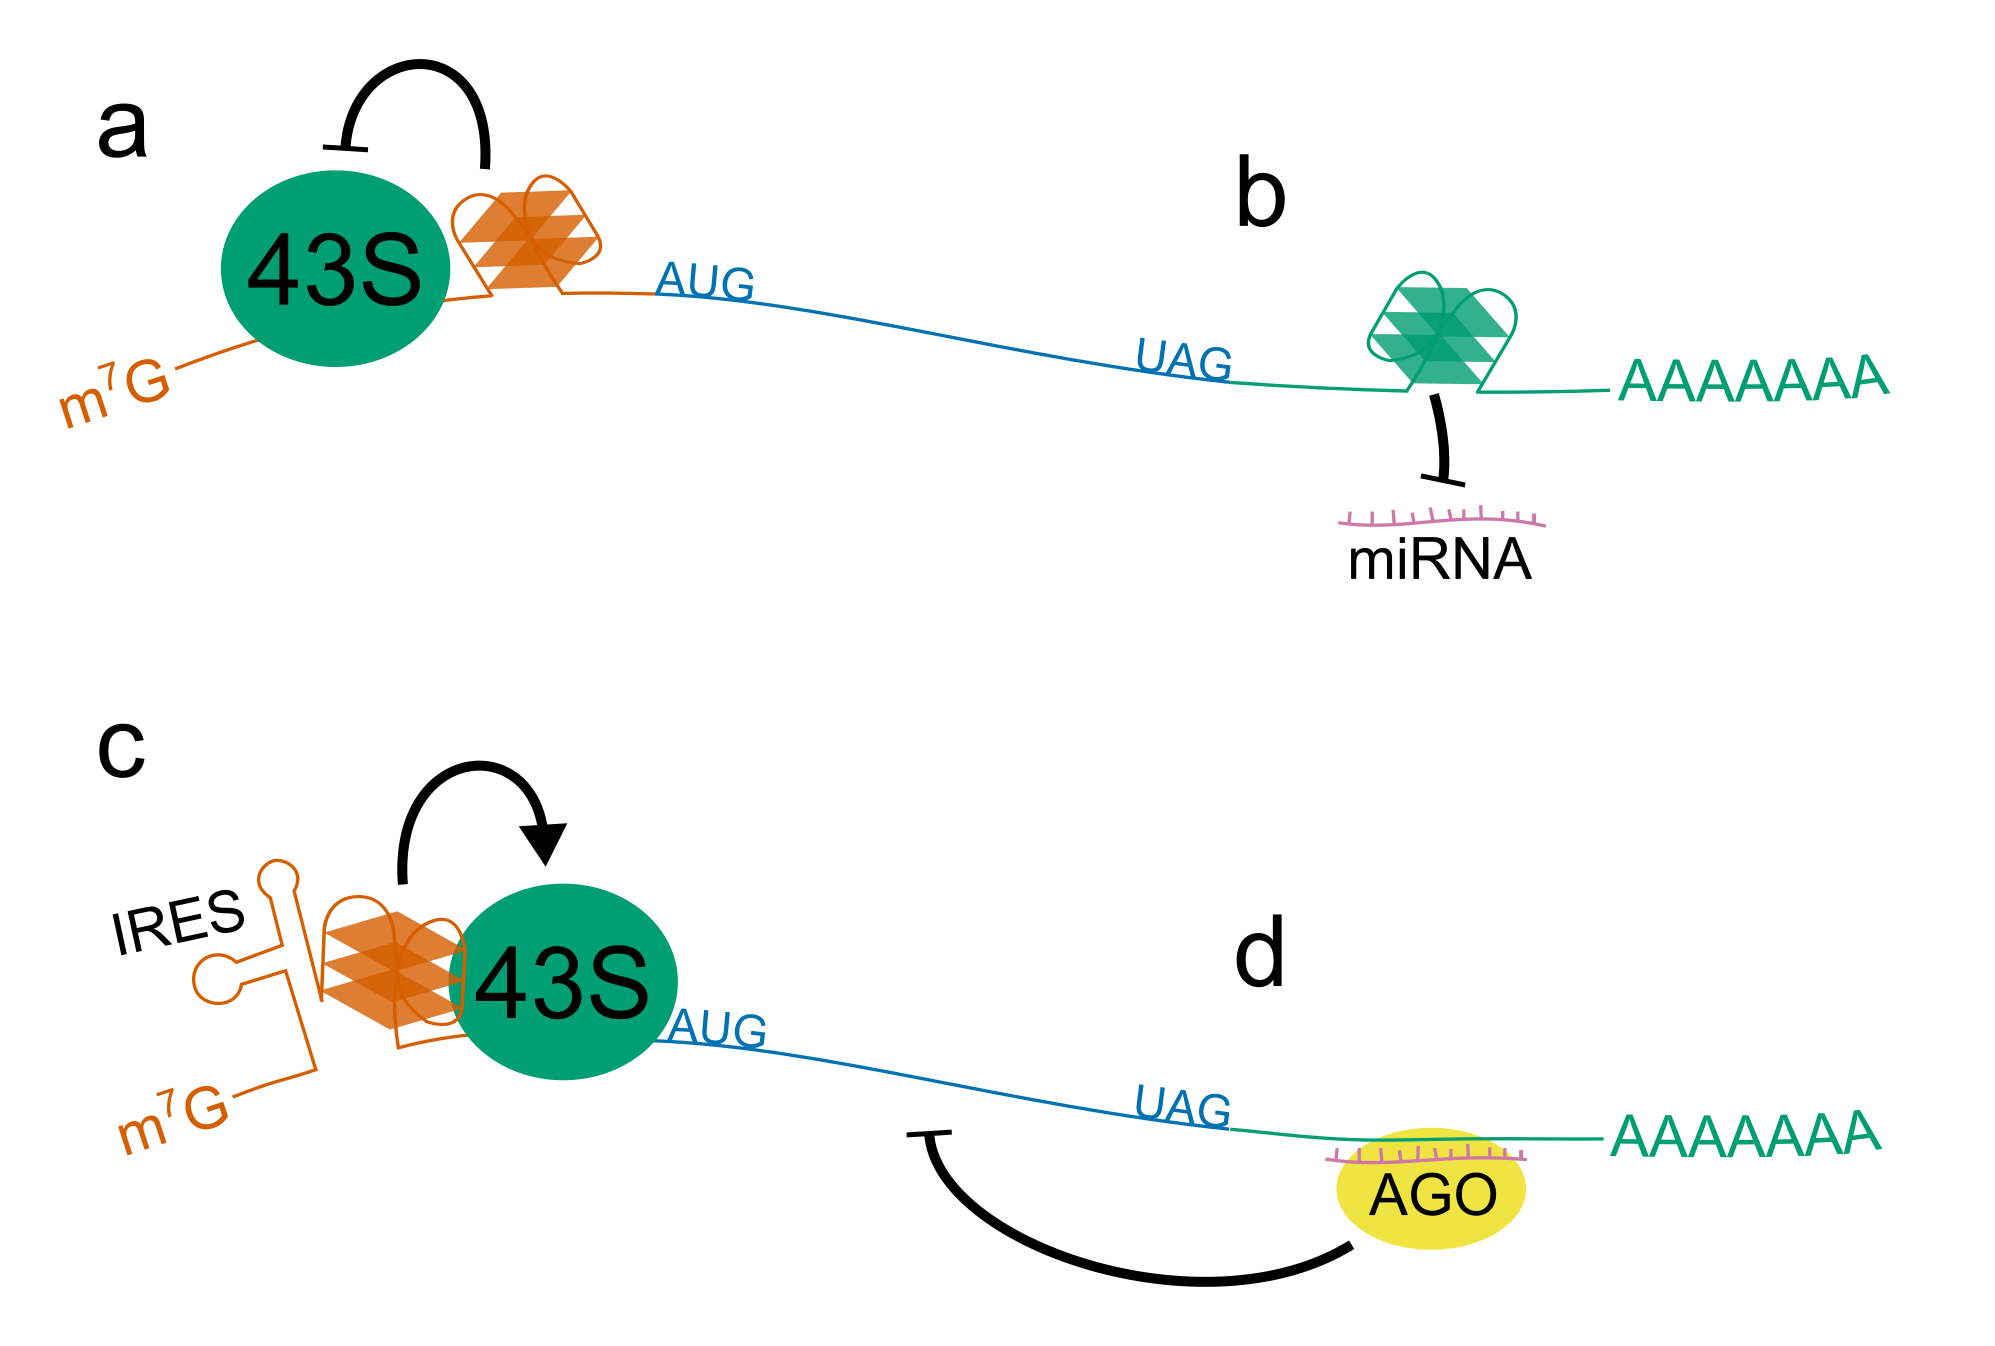
\includegraphics[width=\textwidth,height=562pt,keepaspectratio]{introduction/figures/mRNA_stability_translation.png}
\caption[G4 function in translation and mRNA stability]{\textbf{G4   function   in   translation   and   mRNA   stability}   Schematic   showing   how   5’   and   3’   UTR   G4s   can   effect   translation   of   mRNAs.   \textbf{a)}   G4s   in   the   5’   UTR   of   mRNAs   can   cause   a   reduction   in   gene   expression   by   preventing   scanning   of   the   PIC   along   the   UTR.   \textbf{b)}   and   \textbf{d)}   G4   formation   in   the   3’UTR   could   block   the   recognition   of   miRNA   binding   sites   by   Argonaute   proteins.   \textbf{c)}   G4s   which   form   in   long   and   structured   5’   UTRs   can   contribute   to   internal   ribosome   entry   site   (IRES)   which   promote   cap   independent   initiation   of   translation}
\end{figure}

\newpage

\hypertarget{epigenetics-and-chromatin-remodelling}{%
\subsection{Epigenetics and Chromatin
Remodelling}\label{epigenetics-and-chromatin-remodelling}}

\label{ssec:chromatin}

Chromatin conformational dynamics are important regulatory mechanisms
for gene expression. The major protein component of chromatin is made up
of histones, which assemble into the nucleosomes around which DNA is
wrapped. G4 formation is highly dependent upon chromatin status, and G4s
isolated by BG4 ChIPseq have been shown to form in regions of open
chromatin (Hänsel-Hertsch et al., 2016). Hänsel-Hertsch et al.~showed
that treatment of cells with the histone deacetylase inhibitors, which
cause a relaxation of the chromatin, also increased the number of G4
loci identified by ChIPseq (Hänsel-Hertsch et al., 2016).

\textless{}\textless{}\textless{}\textless{}\textless{}\textless{}\textless{}
Updated upstream G4s have been shown to cause transient and
non-heritable changes to epigenetic status through the causing of DSB,
which are known to induce phosphorylation of H2AX (gamma-H2AX) via an
ATM-dependent pathway (Shanbhag et al., 2010; Rodriguez et al., 2012;
Ayrapetov et al., 2014). A number of authors have also reported
heritable epigenetic changes to the BU-1 and beta-globin gene loci
caused by G4s in chicken cell lines (Sarkies et al., 2010, 2012;
Schiavone et al., 2014, 2016; Guilbaud et al., 2017). These changes
occur in cells lacking G4 resolving helicases, such as REV1, FANCJ, WRN
and BLM (Sarkies et al., 2010, 2012; Eddy et al., 2014; Schiavone et
al., 2014); polymerases, such as PrimPol (Schiavone et al., 2016); or in
cells treated with G4 stabilising agents, such as NMM, PhenDC3 and PDS
(Guilbaud et al., 2017). None of these conditions caused DSB or
mutations in the BU-1 gene, but did cause loss of active chromatin
marker H3K4me3, and gain of repressive H3K9me3, as well as an increase
in repressive DNA methylation. There was a concommitant decrease in gene
expression accompanying these changes (Sarkies et al., 2010, 2012;
Schiavone et al., 2014, 2016; Guilbaud et al., 2017). During
replication, parental histones from upstream of the replication fork are
removed; and recycled into the newly synthesised DNA behind the
replication machinery (De Koning et al., 2007). This recycling maintains
the epigenetic status of replicated DNA. Sarkies et al.~proposed that in
the absence of G4 unwinding helicases, or in the presence of a
stabilising drug, leading strand synthesis is stalled at the G4, and
uncoupled from histone recycling. This leads to the incorporation of
newly synthesised H3/4 without the correct epigenetic markers, rather
than parental histones (Sarkies et al., 2010, 2012; Schiavone et al.,
2014, 2016; Guilbaud et al., 2017). Abolishment of the G4 motif through
mutation removed this heritable change in epigenetic status.
Furthermore, switching of the strand of the G4, which was suggested to
switch the replication strand of the G4 from the leading to the lagging
strand, also abolished the heritable change in expression (Sarkies et
al., 2010, 2012; Schiavone et al., 2014, 2016).

\newpage

\begin{figure}[htbp]
\centering
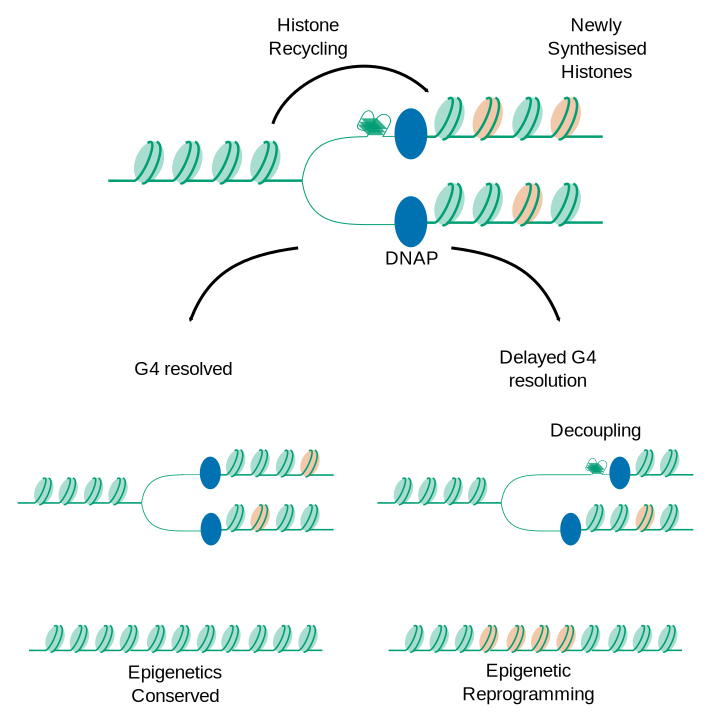
\includegraphics[width=\textwidth,height=562pt,keepaspectratio]{introduction/figures/histone_recycling.png}
\caption[G4 stalling causes epigenetic reprogramming]{\textbf{G4   stalling   causes   epigenetic   reprogramming}   Illustration   demonstrating   the   mechanism   by   which   G4   stalling   is   thought   to   cause   epigenetic   reprogramming.   Histone   recycling   from   upstream   of   the   replication   fork   into   newly   synthesised   DNA   is   tightly   linked   to   DNA   replication.   This   is   important   to   maintain   the   correct   histone   modifications   in   the   daughter   cells.   When   G4s   form   in   the   leading   strand   of   the   DNA,   they   cause   blockages   that   decouple   DNA   replication   from   histone   removal,   resulting   in   the   insertion   of   newly   synthesised   histones   into   the   DNA.   This   causes   the   loss   of   histone   modifications   from   this   region   of   the   DNA.}
\end{figure}

\hypertarget{section}{%
\chapter{\texorpdfstring{\newpage}{}}\label{section}}

G4s have been shown to cause transient and non-heritable changes to
epigenetic status through the causing of DSB, which are known to induce
phosphorylation of H2AX (gamma-H2AX) via an ATM-dependent pathway
(Shanbhag et al., 2010; Rodriguez et al., 2012; Ayrapetov et al., 2014).
A number of authors have also reported heritable epigenetic changes to
the BU-1 and beta-globin gene loci caused by G4s in chicken cell lines
(Sarkies et al., 2010, 2012; Schiavone et al., 2014, 2016; Guilbaud et
al., 2017). These changes occur in cells lacking G4 resolving helicases,
such as REV1, FANCJ, WRN and BLM (Sarkies et al., 2010, 2012; Eddy et
al., 2014; Schiavone et al., 2014); polymerases, such as PrimPol
(Schiavone et al., 2016); or in cells treated with G4 stabilising
agents, such as NMM, PhenDC3 and PDS (Guilbaud et al., 2017). None of
these conditions caused DSB or mutations in the BU-1 gene, but did cause
loss of active chromatin marker H3K4me3, and gain of repressive H3K9me3,
as well as an increase in repressive DNA methylation. There was a
concommitant decrease in gene expression accompanying these changes
(Sarkies et al., 2010, 2012; Schiavone et al., 2014, 2016; Guilbaud et
al., 2017). During replication, parental histones from upstream of the
replication fork are removed; and recycled into the newly synthesised
DNA behind the replication machinery (De Koning et al., 2007). This
recycling maintains the epigenetic status of replicated DNA. Sarkies et
al.~proposed that in the absence of G4 unwinding helicases, or in the
presence of a stabilising drug, leading strand synthesis is stalled at
the G4, and uncoupled from histone recycling. This leads to the
incorporation of newly synthesised H3/4 without the correct epigenetic
markers, rather than parental histones (Sarkies et al., 2010, 2012;
Schiavone et al., 2014, 2016; Guilbaud et al., 2017). Abolishment of the
G4 motif through mutation removed this heritable change in epigenetic
status. Furthermore, switching of the strand of the G4, which was
suggested to switch the replication strand of the G4 from the leading to
the lagging strand, also abolished the heritable change in expression
(Sarkies et al., 2010, 2012; Schiavone et al., 2014, 2016).
\textgreater{}\textgreater{}\textgreater{}\textgreater{}\textgreater{}\textgreater{}\textgreater{}
Stashed changes

Chromatin remodelling is the process by which modifications are made to
histones. These modifications include switching of histone isoforms,
covalent modifications, and histone sliding. The latter involves the use
of energy from ATP hydrolysis to translocate histones along the DNA
polymer without ever removing them (Längst and Manelyte, 2015). One
class of remodellers is SWI/SNF complexes, which are able to slide or
eject nucleosomes. ATRX is an X-linked SWI/SNF family member, which is
mutated in ATR-X syndrome, an intellectual disability disorder. The ATRX
protein has been shown to locate at heterochromatic and pericentromeric
regions, as well as at telomeres (McDowell et al., 1999), regions which
are enriched in G-rich PG4 structures. During ATR-X syndrome, global DNA
methylation patterns at these regions are disregulated (Gibbons et al.,
2000). Knockdown of ATRX during the S-phase of the cell cycle, when DNA
replication occurs, results in an increase in the DSB response marker
gamma-H2AX at telomeric regions (Wong et al., 2010). Heaphy et
al.~showed that human pancreatic cancers which had lost the expression
of ATRX or its partner protein DAXX had elongated telomeres that were
characteristic of the Alternative Lengthening of Telomeres pathway. This
pathway is telomerase independent, suggesting that ATRX is important for
normal telomere repair (Heaphy et al., 2011).

ATRX mutation also effects gene expression. Gibbons et al.~identified
gene expression changes in the alpha globin gene cluster in response to
ATRX mutation (Gibbons et al., 1991). More recently, Law et
al.~performed ChIP-seq using an ATRX specific antibody to identify other
gene targets. They found that ATRX binds specifically to G-rich tandem
repeats which form G4s \emph{in vitro}. Furthermore, the strength of the
effect of ATRX mutation on gene expression was proportional to the
number of tandem G-rich repeats. This suggests that the effect is
increased by the number or stability of G4s (Law et al., 2010).

\newpage

\hypertarget{r-loop-biology}{%
\subsection{R loop Biology}\label{r-loop-biology}}

\label{ssec:rloop_csr}

R loops have been characterised \emph{in vitro} in a number of
organisms, from initial studies in \emph{E. coli} (Drolet et al., 1995)
to genome wide profiling in \emph{S. cerevisiae} (Chan et al., 2014) and
\emph{H. sapiens} cell lines (Chen et al., 2017). R loops have been
implicated in maintaining chromatin status and gene expression (Powell
et al., 2013; Chen et al., 2015), as well as termination of
transcription (Skourti-Stathaki et al., 2011, 2011). Chen et al.~used an
inactive RNase H enzyme, which binds specifically to RNA:DNA
heteroduplexes, to immunoprecipitate R-loops in human chromatin (Chen et
al., 2017). They identified a large number of R loop peaks located at
promoter proximal regions, suggesting R loop formation early in
transcription. The authors found that R loops were more common on genes
that showed higher levels of proximal pausing, suggesting that R loop
formation may be associated with the pausing of Pol II (Chen et al.,
2017). Furthermore, regions containing R loops were also strongly
associated with coding strand G4s, with 54\% of R loop peaks containing
a G4 observed by G4seq (Chambers et al., 2015; Chen et al., 2017). G4
formation in the coding strand, which is in a single stranded state in
the R loop, may help to stabilise the RNA:DNA hybrid (Duquette et al.,
2004).

R loop formation has been identified as a key component of class switch
recombination (CSR) of immunoglobulin genes (Reaban and Griffin, 1990;
Daniels and Lieber, 1995; Yu et al., 2003). CSR is the process by which
the constant region of the immunoglobulin heavy chain (IgH) gene is
switched, changing the properties of the resultant antibody (Stavnezer,
1996). This process is mediated by the activation-induced cytidine
deaminase (AID), an enzyme which deaminates cytosines in ssDNA, within
the switch regions of the IgH locus. This deamination results in DSB,
causing the recombination of the gene. Transcription of the IgH gene
produces a long non-coding RNA (lncRNA) with a constitutive first exon
containing the variable antigen binding domain. Splicing to an
alternative second exon is determined by the pattern of cytokines that
the cell is exposed to. The intron lariat removed by this splicing is
debranched and re-linearised by the enzyme DBR1 (Zheng et al., 2015).
This intron lariat then forms an R-loop with the switch region of the
IgH, resulting in ssDNA on the coding strand which becomes the substrate
for AID. Zheng et al.~showed that AID is able to bind specifically to G4
DNA and RNA, and that targeting of AID to the switch region is via
binding to the debranched RNA lariat (Zheng et al., 2015). Furthermore,
Ribeiro de Almeida et al.~identified that resolution of G4s in the
intron derived RNA is required for R-loop formation and CSR. This G4
unwinding was found to occur via the RNA Helicase DDX1 (Ribeiro de
Almeida et al., 2018).

\newpage

\begin{figure}[htbp]
\centering
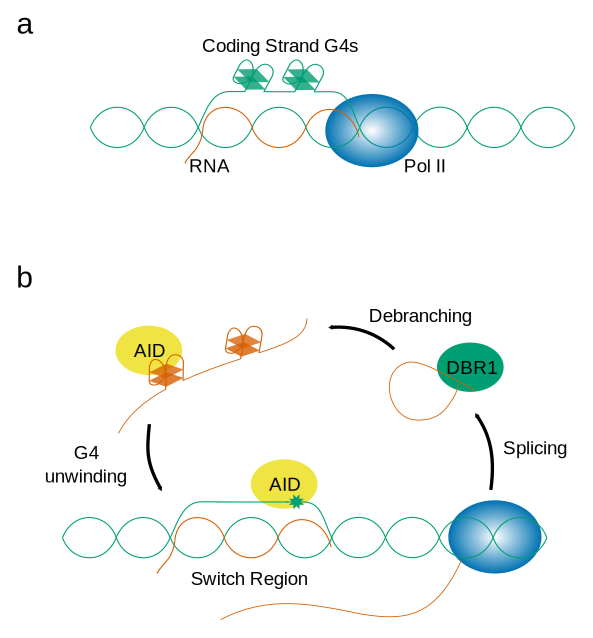
\includegraphics[width=\textwidth,height=562pt,keepaspectratio]{introduction/figures/rloops.png}
\caption[An R-loop and G4 dependent mechanism for Class Switch Recombination]{\textbf{An   R-loop   and   G4   dependent   mechanism   for   Class   Switch   Recombination}   \textbf{a)}   Schematic   showing   the   formation   of   an   R-loop   from   G-rich   RNA   and   C-rich   template   DNA,   behind   transcribing   RNA   Polymerase   II.   The   G-rich   coding   strand   is   left   in   a   single   stranded   form,   and   may   fold   into   G4s.   \textbf{b)}   Proposed   mechanism   for   Class   Switch   Recombination   of   IgH   gene   through   R-loop   formation.   Transcription   and   splicing   of   the   IgH   locus   results   in   a   G-rich   intron   lariat   which   is   debranched   by   DBR1.   This   folds   into   RNA   G4s   which   recruit   AID.   Resolution   of   G4s   by   DDX1   promotes   R   loop   formation   and   targets   AID   to   the   switch   region,   causing   deamination   and   double   strand   breaks.}
\end{figure}

\newpage

\hypertarget{role-of-g-quadruplexes-in-planta}{%
\section{\texorpdfstring{Role of G-Quadruplexes \emph{in
planta}}{Role of G-Quadruplexes in planta}}\label{role-of-g-quadruplexes-in-planta}}

\label{sec:g4s_in_plants}

\hypertarget{g-quadruplex-distribution}{%
\subsection{G-Quadruplex Distribution}\label{g-quadruplex-distribution}}

\label{ssec:plant_distribution}

Whilst the majority of G4 studies have been performed in mammalian
systems, particularly \emph{H. sapiens}, there is a growing body of
evidence for functions of G4s in plant species including
\emph{Arabidopsis thaliana}, \emph{Zea mays}, and \emph{Oryza sativa}
(Mullen et al., 2010; Takahashi et al., 2012; Andorf et al., 2014; Wang
et al., 2014; Garg et al., 2016; Yadav et al., 2017). Monocotyledonous
flowering plants such as \emph{O. sativa} and \emph{Z. mays} generally
have higher GC content than dicotyledonous flowering plants and
non-flowering plants (Šmarda et al., 2014). Monocots also have higher
PG4 content, presumably as a result of this (Garg et al., 2016). Three
tetrad PG4 densities of plants tend to be lower than those of the well
studied \emph{H. sapiens} and \emph{M. musculus}, however.
\emph{Arabidopsis thaliana}, the model plant, has a small genome and low
PG4 density, with only 1200 three tetrad PG4s (Mullen et al., 2010).
This represented a greater than two fold depletion of PG4s over what was
expected in a windowed markov chain modelled genome (Mullen et al.,
2010). Mullen et al.~noted that Arabidopsis contains 43000 two tetrad
PG4s, however, which they suggested might be stable at the temperature
ranges that Arabidopsis lives at (Mullen et al., 2010, 2012). Garg et
al.~identified 1331 genes which have conserved two tetrad or greater
PG4s in all dicot species tested, suggesting functional conservation of
these motifs (Garg et al., 2016). Takahashi et al.~analysed the plant
species \emph{O. sativa}, \emph{P. trichocarpa}, \emph{V. vinifera} and
\emph{A. thaliana}, and found an enrichment of PG4s at the TSS of genes,
particularly on the template strand of the gene (Takahashi et al.,
2012).

\hypertarget{g-quadruplexes-in-plant-telomeres}{%
\subsection{G-Quadruplexes in plant
telomeres}\label{g-quadruplexes-in-plant-telomeres}}

Arabidopsis telomeres are made up of the heptameric sequence TTTAGGG
(Richards and Ausubel, 1988). This is slightly different sequence repeat
from that found in most vertebrates, including \emph{H. sapiens} (Kim
and Kim, 2018). A number of plants species have also been reported to
contain the same TTAGGG repeat as vertebrates, however (Kim and Kim,
2018). Both Arabidopsis and \emph{O. sativa} have been shown to be
sensitive to the telomerase inhibitor telomestatin (Zhang et al., 2006).
Telomestatin is a G4 binding agent which has been shown to interact with
the human telomeric repeat, and inhibit telomerase causing telomere
shortening \emph{in vivo} (Kim et al., 2002). Zhang et al.~showed that
sensitivity of cultured Arabidopsis and \emph{O. sativa} cells to
telomestatin occurs via the same method of telomere shortening,
suggesting that plant telomeres may also form G4s \emph{in vivo} (Zhang
et al., 2006).

\hypertarget{transposable-elements}{%
\subsection{Transposable Elements}\label{transposable-elements}}

Transposable elements (TEs) are discrete regions of DNA which are able
to copy or translocate themselves from one region of the genome to
another (Kejnovsky et al., 2015). The most common family of plant TEs
are long terminal repeat (LTR) retrotransposons, which duplicate
themselves through transcription followed by reverse transcription
(Kejnovsky et al., 2015). Lexa et al.~have shown that plant LTR
retrotransposons are enriched in motifs which form G4s \emph{in vitro}
(Lexa et al., 2014). These are most commonly found in the LTRs of the
TEs, at the 5' end in the positive strand and at the 3' end in the
negative strand (Lexa et al., 2014). The authors also noted that younger
TEs with greater homology between LTRs were also more likely to contain
PG4s with longer G-runs. They argued that this suggests a function for
G4s in the life cycle of the TE (Lexa et al., 2014). Tokan et al.~also
demonstrated that treatment of \emph{Z. mays} with the G4 stabilising
drug NMM caused downregulation of some highly expressed LTR
retrotransposons (Tokan et al., 2018). Kejnovsky and Lexa identified
that G4s are also common in LTR fragments which occur throughout plant
genomes as a result of ectopic recombination (Kejnovsky and Lexa, 2014).
This is a potential mechanism for the introduction of G4s into new
regions of the genome, where they may evolve some evolutionary purpose
(Kejnovsky and Lexa, 2014).

\hypertarget{translational-regulation}{%
\subsection{Translational Regulation}\label{translational-regulation}}

\label{ssec:plant_translation}

An enrichment of PG4s in 5' UTRs has been identified in a number of
plant species, including \emph{A. thaliana} (Mullen et al., 2010; Garg
et al., 2016), \emph{Z. mays} (Andorf et al., 2014), and \emph{O.
sativa} (Wang et al., 2014). Several of these have been shown to form in
RNA (Kwok et al., 2015; Cho et al., 2018). Kwok et al.~identified a PG4
motif on the coding strand of the ATR gene in Arabidopsis, which forms
in the 5' UTR of the mRNA (Kwok et al., 2015). They showed using a
transient reporter gene assay that this G4 inhibits translation, but not
transcription, presumably by preventing scanning of the UTR by the
ribosomal PIC (Kwok et al., 2015).

Cho et al.~also identified an RNA G4 which forms in the 5'UTR of
SMXL4/5, a gene involved in the differentiation of the phloem (Cho et
al., 2018). They found that this G4 was bound and stabilised by the G4
binding protein JULGI. Using SELEX, they showed that JULGI was able to
bind a number of PG4 forming sequences (Cho et al., 2018). G4 formation
in the SMXL4/5 5'UTR resulted in a reduction of the translation of mRNA,
and a restriction of the phloem, whilst knockout of JULGI strongly
promoted phloem development (Cho et al., 2018). A PG4 motif was
identified in the 5'UTR of SMXL4/5 in all vascular plants analysed,
suggesting that this mechanism was evolved early in the development of
vascular plants (Cho et al., 2018).

\hypertarget{plant-development}{%
\subsection{Plant Development}\label{plant-development}}

\label{ssec:plant_dev}

Given the evolutionarily ancient role of G4s in phloem development (Cho
et al., 2018), it is plausible that molecular mechanisms involving G4s
are central to many plant development pathways. Nakagawa et al.~analysed
the effects of the G4 binding agents NMM and Berberine on Arabidopsis
development, and found that both drugs caused defects in leaf polarity
(Nakagawa et al., 2012). Furthermore, plants with double mutations in
the genes \emph{ASYMMETRIC LEAVES 1} and \emph{2} were hypersensitive to
G4 binding agents (Nakagawa et al., 2012).

\hypertarget{stress-response}{%
\subsection{Stress Response}\label{stress-response}}

\label{ssec:plant_stress}

Analysis by Mullen et al.~identified that the greatest enrichment of two
tetrads in the Arabidopsis genome was inside genic regions, and that
these PG4s might form in mRNA (Mullen et al., 2010). Furthermore, they
demonstrated that many two tetrad PG4s are only strongly stable in high
potassium concentrations, and postulated that these might act as
molecular switches sensing environmental salt concentrations (Mullen et
al., 2012). Since cellular potassium concentrations are increased from
around 100mM to as much as 600mM during osmotic stresses (e.g.~drought
stress) (Walker et al., 1996; Hummel et al., 2010), they suggested that
drought stress responsive genes could contain these molecular switches.
Yadav et al.~found that 16\% of the Arabidopsis genome is drought
responsive, and of these, 45\% contain PG4s (Yadav et al., 2017).
Analysis of the \emph{Z. mays} genome by Andorf et al.~has also shown
that PG4s are enriched in a number of gene ontology classes involved in
stress response, including hypoxia and nutrient deprivation responsive
genes (Andorf et al., 2014).

\newpage

\hypertarget{summary}{%
\section{Summary}\label{summary}}

\label{ssec:intro_summary}

There is now clear evidence for the \emph{in vivo} function of DNA and
RNA G4s in a wide range of molecular processes, including genome
stability, replication, transcription, mRNA processing, and translation.
In this thesis, we will introduce a new method for the detection of DNA
and RNA G4s, using information learned from high throughput sequencing
datasets (Chambers et al., 2015; Kwok et al., 2016). We will then apply
this and other methods to the detection of PG4s in the Arabidopsis
genome, and identify their enrichment in various genic features
including 5'UTRs and CDSs. Finally, we will attempt to identify the
effect of G4 stabilisation on Arabidopsis gene expression by treating
plants with the G4 binding agent NMM. We will attempt to shed some light
on whether the G4 rich genes affected by NMM are naturally regulated
through G4 dependent mechanisms.

\newpage

\hypertarget{a-recurrent-neural-network-to-predict-g-quadruplex-structure}{%
\chapter{A Recurrent Neural Network to Predict G Quadruplex
Structure}\label{a-recurrent-neural-network-to-predict-g-quadruplex-structure}}

\label{chap:g4seeqer}

\hypertarget{introduction-1}{%
\section{Introduction}\label{introduction-1}}

Because of the dependence of G4 structure largely on sequence
information, it is possible to make predictions about the propensity of
specific sequences to form G4s using pattern matching analyses. The
initial rule which was employed for putative G4 (PG4) detection in the
human genome was the Quadparser method (Huppert and Balasubramanian,
2005). This is a simple regular expression following the pattern
\(G_{X}N_{1-7}G_{X}N_{1-7}G_{X}N_{1-7}G_{X}\) where \(X\geqslant 3\).
The Quadparser method was chosen based upon early Circular Dichroism and
UV melting data, which suggested that G4s tended to be more stable with
three or more tetrads, relatively short loop lengths, and no bulges in
tetrads. These fairly stringent rules for formation mean that in
general, the Quadparser method is considered to be fairly conservative,
and misses a lot of sequences with high G4 forming potential.

More recently there has been a large increase in the number of available
methods for predicting G4s (Bedrat et al., 2016; Garant et al., 2017;
Hon et al., 2017; Sahakyan et al., 2017). The contribution from Bedrat
et al., named G4Hunter, is a scoring method based on a run length
encoding the input sequence. Runs of Gs score positively whilst runs of
Cs score negatively. It can be used with a sliding window approach to
score an entire genome, with thresholding to identify high scoring PG4s.
Whilst this approach is much more tolerant of imperfections which
violate the Quadparser method, it is arguably too tolerant, producing
many false positives. Furthermore, it does not take into account
flanking A and T sequences which may contribute to the stability of the
G4, e.g.~through reducing the favourability of double stranded DNA.

Some middle ground is required to improve existing methods. The key to
finding this middle ground may come from the fields of data science and
machine learning. There is a current global interest in machine learning
approaches, due to increases in computational power which allow larger
datasets to be analysed. These techniques have been adopted by
bioinformaticians for making global predictions of functional sequences
such as splice sites or transcription factor binding motifs. For
example, Mapleson et al.~have developed a tool called
\texttt{portcullis} which is able to filter out spurious splice sites
caused by mapping errors from RNAseq data. This is done by training a
random forest model on the fly using features derived from high and low
confidence splice sites in the dataset. The trained model is then used
to classify all other ambiguous splice sites in the dataset as either
true or false positives (Mapleson et al., 2017). Neural networks have
also been used to identify sequence motifs. Alipanahi et al.~developed a
convolutional neural network called \texttt{DeepBind} which they applied
to identify transcription factor binding motifs and other regulatory
sequences, using data from Protein binding microarrays (PBMs), SELEX or
ChIP-seq for training (Alipanahi et al., 2015). Quang et al.~were able
to improve on this model by using a hybrid convolutional and recurrent
neural network (Quang and Xie, 2016). This neural network architecture
will be explained in detail in \autoref{ssec:results_model_choice}.

Machine Learning approaches have already been brought to bear on the
problem of G4 prediction. For example, Garant et al.~developed G4RNA
screener, a densely connected neural network which is trained on the
trinucleotide contents of input sequences (Garant et al., 2017). This
model was trained by using a set of melting temperatures of RNA G4s
obtained from a literature search. Currently this database contains only
368 sequences, however. Given the almost inconceivable number of
potential G4 forming sequences (there are more than \(10^{12}\)
sequences which could match the original Quadparser pattern, not
including flanking sequences), it is probable that this dataset does not
capture all of the variety of possible RNA G4 forming sequences. To do
this, a more high throughput method for measuring G4 forming propensity
is required.

A new method for sequencing of genomic G4 structures, termed G4Seq, may
provide this level of throughput (Chambers et al., 2015). To create this
dataset, Chamber et al.~sequenced human genomic DNA in an Illumina
sequencing-by-synthesis machine, in the presence or absence of G4
stabilising potassium cations, or G4 binding ligand Pyridostatin. The G4
structures caused stalling of DNA polymerase, resulting in a large
number of errors in the resulting read. When the authors then mapped the
resultant reads, the mismatch rate which occurred at each position in
the genome could be counted to create a map of G4-forming loci. Another
high throughput method for sequencing G4s, this time in human mRNAs, was
developed by Kwok et al.~This protocol utilises the ability of potassium
or pyridostatin stabilised RNA G4s to stall reverse transcriptase,
resulting in a drop off of reads in the 3'-\textgreater{}5' direction in
RNAseq data (Kwok et al., 2016).

Data from the G4Seq experiment was leveraged by Sahakyan et al.~to build
an extreme gradient boosted machine model, named Quadron, to predict G4
formation (Sahakyan et al., 2017). Quadron initially predicts PG4s using
the Quadparser method, but with extended loop lengths of 1-12. Various
derived features, such as tetrad number, loop length and mono-, di- and
trinucleotide content, are then extracted from these patterns and used
to train a model predicting G4Seq mismatch rate. The primary drawback of
this method is that the Quadparser method is still used to make initial
predictions. This means that Quadron is only able to improve the
precision of the existing Quadparser method by rejecting false positives
that do not form G4s. Since the Quadparser method is already quite
conservative, a lot of potential G4 forming sequences are still missed.

Here we present a new method for G4 prediction, which builds on the work
of Bedrat et al.~and Sahakyan et al.~We use the G4Seq dataset as
training data, however a convolutional and recurrent neural network is
used to process input sequences directly, meaning fewer prior
assumptions are required about what constitutes a G4 forming sequence.
Our new method, which we name G4Seeqer, performs better on both the
G4Seq datasets and other datasets, including G4s immunoprecipitated from
chromatin (Hänsel-Hertsch et al., 2016). We also use transfer learning
to apply the model learned from G4Seq data to RNA G4 prediction.
Finally, we use G4Seeqer to characterise unnoticed features of the G4Seq
dataset, and compare our scores to data from UV melting experiments.

\newpage

\hypertarget{materials-and-methods}{%
\section{Materials and Methods}\label{materials-and-methods}}

\hypertarget{g4hunter-algorithm}{%
\subsection{G4Hunter Algorithm}\label{g4hunter-algorithm}}

The G4hunter algorithm from Bedrat et al.~was reimplemented in Cython
(Python superset which can be compiled to C) with some alterations
(Bedrat et al., 2016). Input sequences were run length encoded, and each
run of Gs was scored as the square of length of the run, with a maximum
score per run of 16. These scores were summed to give a positive strand
total score. Runs of Cs were scored equivalently but in a separate
negative strand score. Scores were divided by the length of the input
sequence to get a normalised score.

\hypertarget{training-data-preprocessing}{%
\subsection{Training Data
Preprocessing}\label{training-data-preprocessing}}

The modified G4Hunter method was run on the hg19 genome using a window
size of 50bp, a step size of 5 and a threshold of 0.75 to generate a
total of 7484506 candidate G4 intervals, which were output in bed
format. Intervals were increased in size by 39bp in each direction using
\texttt{bedtools\ slop} to introduce flanking sequence information for
classification (Quinlan and Hall, 2010). Overlapping intervals were
filtered to yield the greatest number of non-overlapping intervals.
Intervals were weighted by their G4Hunter score, such that the maximum
number of high scoring non-overlapping intervals was yielded.

To ground truth score these sequences, \texttt{bedtools\ map} was used
to intersect them with the G4Seq dataset (Chambers et al., 2015), which
was downloaded from GEO (GSE63874). Bedgraph files of this data
contained percentage mismatch scores for each position of the human
genome at 15bp resolution. The G4Seq dataset generated in the presence
of potassium was chosen as it was deemed more likely to be of biological
relevance than the dataset generated in the presence of Pyridostatin, a
G4-binding drug.

Intervals files and corresponding mismatch scores were read into Python
using \texttt{pandas} and histograms of log transformed mismatch scores
were plotted using \texttt{matplotlib} (VanRossum, 1995; Hunter, 2007;
Mckinney, 2011). The threshold of approximately 3 for separating
G4-forming and non-G4 forming sequences was chosen using \texttt{scipy}
to determine the local minimum in the histogram (Jones et al., 2001).
Joint plots of percentage mismatch score against G4Hunter score were
plotted using \texttt{seaborn} (Waskom et al., 2014).

Since positive training examples were outweighed by negative ones in
this dataset by a factor of 10:1, random under-sampling of negative
examples was conducted using \texttt{imblanced-learn} to attain a ratio
of 2:1 (Lemaître et al., 2001). This filtered dataset was shuffled and
written to disk in bed format, and \texttt{bedtools\ getfasta} was used
to extract sequences for each interval from hg19 (Quinlan and Hall,
2010). Sequences were then one hot encoded, i.e.~represented as binary
matrices of size 128x4, and loaded into HDF5 format for training using
\texttt{h5py} (Andrew Collette, 2013). For training of models on
trinucleotide content, trinucleotide content statistics were extracted
and loaded into HDF5 format.

\hypertarget{model-training-and-validation}{%
\subsection{Model Training and
Validation}\label{model-training-and-validation}}

All models were trained in Python using \texttt{Keras} with
\texttt{TensorFlow} backend (Abadi et al., 2016; Chollet, 2018). The
trinucleotide Multi-Layer Perceptron (MLP) model contained three hidden
layers with 16 units per layer. These were trained using the ADAM
optimiser and binary crossentropy loss function, with a dropout rate of
0.2 on all layers. The convolutional portion of G4Seeqer was made up of
two convolutional layers with 8 filters and kernel size of 3 and ReLu
activation, followed by a maximum pooling layer with step size of 2.
This was connected to a bidirectional Long Short Term Memory layer with
8 units and Tanh activation. The final hidden layer was a fully
connected layer with 16 units, ReLu activation and a dropout rate of
0.5. G4Seeqer was trained using the RMSprop optimiser and binary
crossentropy loss function.

All models were trained on 80\% of the training data with 10\% used for
validation. Training was conducted for a maximum of 30 epochs, but with
early stopping when the change in validation loss was less than 0.0005
for more than 3 Epochs. The densely connected network (also known as a
Multi Layer Perceptron or MLP) trained on trinucleotide contents
converged to this minimum change after 8 Epochs, whilst G4Seeqer
converged after 15 Epochs.

Models were validated on 10\% of the total data held out for testing
purposes. Receiver Operator Characteristic (ROC) and Precision Recall
(PR) curves were generated using \texttt{scikit-learn} and plotted with
\texttt{matplotlib} (Hunter, 2007; Pedregosa et al., 2011). ROC/PR
curves for G4Hunter are produced using the modified method. For
comparison against Quadron, the Quadron source code was downloaded from
GitHub and installed (Sahakyan et al., 2017). Since the flanking
sequences required for Quadron are longer than those used for G4Seeqer,
test set sequences were increased in size by 50bp in each direction to
228bp. Sequences were extracted using \texttt{bedtools\ getfasta} and
run through Quadron (Quinlan and Hall, 2010). For intervals which
contained multiple Quadron scoring motifs, the highest score was used.
For intervals which had no motifs scored by Quadron, a score of zero was
assigned.

\hypertarget{bg4-analysis}{%
\subsection{BG4 Analysis}\label{bg4-analysis}}

NarrowPeak BED files of BG4 ChIP-seq peaks were downloaded from GEO
accession GSE76688 (Hänsel-Hertsch et al., 2016). To accommodate
Quadron's flanking sequence requirements, the size of the BG4 intervals
was increased by 50bp in each direction using \texttt{awk} (Aho et al.,
1988). A BG4-negative peak set was generated using
\texttt{bedtools\ shuffle} (Quinlan and Hall, 2010). Shuffling was
performed such that an equal number of simliarly sized intervals were
selected that excluded gaps in the genome or BG4-positive peaks.
Positive and negative peaks were concatenated and sequences were
extracted using \texttt{bedtools\ getfasta} (Quinlan and Hall, 2010).
Predictions were made on these sequences using
G4Seeqer/G4Hunter/Quadron, and the maximum scoring interval overlapping
each peak was assigned as the overall score of the peak. Where a model
did not make any predictions in a peak, it was assigned a score of zero.
Receiver Operator Characteristic (ROC, false positive rate plotted
against true positive rate) and Precision Recall (PR, precision plotted
against recall) curves were generated using \texttt{scikit-learn} and
plotted with \texttt{matplotlib} (Hunter, 2007; Pedregosa et al., 2011).

\hypertarget{rg4seq-training-data-preprocessing}{%
\subsection{rG4seq Training Data
Preprocessing}\label{rg4seq-training-data-preprocessing}}

To produce training data for rG4seeqer, G4hunter windows were predicted
in hg19 using a window size of 50bp and a threshold of 0.75. These were
intersected with human exons using \texttt{bedtools} to get a set of
186279 putative RNA G4 forming sequences. RNA G4s identified by rG4seq
in the presence of potassium (Kwok et al., 2016) were downloaded from
GSE77282 (\texttt{GSE77282\_K\_hits.bed.gz}), and intersected with the
G4hunter windows to identify RNA G4 positive and negative examples. Of
the 3383 identified RNA G4s in the rG4seq dataset, 2811 (83\%)
overlapped with G4hunter windows. Since the ratio of negative to
positive examples was extremely high, negative examples were
undersampled to a ratio of 2:1 using \texttt{imbalanced-learn} (Lemaître
et al., 2001). These were then shuffled and written to disk in bed
format, and \texttt{bedtools\ getfasta} was used to extract sequences
for each interval from hg19 (Quinlan and Hall, 2010). Sequences were
then one hot encoded and loaded into HDF5 format for training using
\texttt{h5py} (Andrew Collette, 2013).

\hypertarget{rg4seq-transfer-learning}{%
\subsection{rG4seq Transfer Learning}\label{rg4seq-transfer-learning}}

Model weights trained on the G4Seq dataset were reloaded in the same
architecture for training on the rG4seq dataset, using \texttt{Keras}
and \texttt{tensorflow} (Abadi et al., 2016; Chollet, 2018). Weights
from the initial convolutional layers were fixed (i.e.~made
untrainable), and only LSTM weights and final dense weights were
trained. The model was trained on 6014 samples (80\%), validated on 752
samples (10\%), and tested on 752 samples (10\%). Training was conducted
as for G4Seeqer, but for a maximum of 200 epochs, with early stopping
after 25 epochs if validation loss did not improve. Initial learning
rate was set at 0.001 but reduced by a factor of 1/3 after 15 epochs
when no reduction in validation loss was seen.

\hypertarget{comparison-to-g4rna-screener}{%
\subsection{Comparison to G4RNA
Screener}\label{comparison-to-g4rna-screener}}

Supplementary data containing 368 RNA sequences, their experimentally
determined G4 forming status, and their predicted score from G4RNA
Screener were downloaded (Garant et al., 2017). Sequences greater than
128bp were filtered to give a total of 347 sequences. Average rG4Seeqer
and G4Seeqer predictions for these sequences were made by generating
1000 randomly paddings for each sequence, one hot encoding, and
performing forward pass through the network. G4RNA Screener scores used
in the ROC curve were taken directly from the supplemental material
(Garant et al., 2017).

\hypertarget{mutation-mapping-analysis}{%
\subsection{Mutation Mapping analysis}\label{mutation-mapping-analysis}}

Mutation mapping was applied to cell type independent human promoter
regions from the ENSEMBL regulatory build (Zerbino et al., 2015), which
was originally generated using \texttt{ChromHMM} (Ernst and Kellis,
2017). Promoter sequences were extracted from hg38. Mutation mapping was
implemented as in Alipanahi et al.~2015: candidate sequences were edited
at each position to each nucleotide, and the resulting sequences were
scored for G4 formation using G4Seeqer (Alipanahi et al., 2015).
Heatmaps were generated in Python using \texttt{seaborn} (Waskom et al.,
2014).

\hypertarget{g-triplex-and-hairpin-analyses}{%
\subsection{G-Triplex and Hairpin
analyses}\label{g-triplex-and-hairpin-analyses}}

G-triplex motifs were predicted in the hg19 genome using an in house
script, using the pattern \(G_XN_{1-4}G_XN_{1-4}G_X\) where
\(3 \leqslant X \leqslant 6\). Candidate triplexes which overlapped with
or were contained within Quadparser motifs (pattern
\(G_{X}N_{1-7}G_{X}N_{1-7}G_{X}N_{1-7}G_{X}\) where
\(3 \leqslant X \leqslant 6\)) were subtracted to produce only triplex
motifs which could not form ``classical'' G4s. To assign mismatch scores
to these sequences, they were increased in size by 50bp in each
direction using \texttt{bedtools\ slop} (Quinlan and Hall, 2010), and
mismatch scores from the G4Seq dataset were mapped using
\texttt{bedtools\ map}. Distances to next G-run were measured in python
using \texttt{pyfaidx} (Shirley et al., 2015).

G-hairpin motifs were predicted in the hg19 genome using the same
script, and the pattern \(G_XN_{1-4}G_X\) where
\(4 \leqslant X \leqslant 6\). Candidate hairpins which overlapped with
or were contained within Quadparser motifs or G-triplex motifs were
filtered. Intervals were increased in size by 50bp in each direction
using \texttt{bedtools\ slop} (Quinlan and Hall, 2010), and mismatch
scores from the G4Seq dataset were mapped using \texttt{bedtools\ map}.
Distances to next G-hairpin were measured using
\texttt{bedtools\ closest}. Triplex and hairpin histograms and boxplots
were generated in Python using \texttt{matplotlib} and \texttt{seaborn}
(Hunter, 2007; Waskom et al., 2014).

\hypertarget{median-model-score-experiments}{%
\subsection{Median model score
experiments}\label{median-model-score-experiments}}

For G4Seeqer scoring of experimentally validated G4s from Guédin et al
2010., sequences were recreated from the information in Table 1, and
padded using uniformly sampled sequences to 128bp in length (Guédin et
al., 2010). Left and right padding lengths were also varied at random.
1000 randomly padded sequences were generated and scored per input
sequence. Scatter plots of UV melting temperature vs.~median G4Seeqer
score were produced using \texttt{matplotlib} (Hunter, 2007). Errorbars
are 68\% confidence intervals calculated from the variation in score for
the same sequence with different random padding.

Synthetic sequences used for loop length and G-register experiments were
generated by combining uniformly sampled padding and loops with GGG
trinucleotides to create 3 tetrad Quadparser conforming sequences. Each
sample contained 5000 randomly generated sequences. Left and right
padding sizes and nucleotide contents for loops were varied within
random samples. Loop nucleotide contents were also varied. For
G-register experiments, the extra G per run was randomly assigned to
either the left of right side of the G-run. Loop lengths of 3 were used.
Line plots for loop length experiments were generated using
\texttt{matplotlib}. Errorbars are 68\% confidence intervals showing the
variation in G4Seeqer score caused by left and right padding size and
padding/loop nucleotide content, when holding loop lengths constant
(Hunter, 2007). Boxplots were generated using \texttt{seaborn} (Waskom
et al., 2014).

\hypertarget{g-register-experiments}{%
\subsection{G-register Experiments}\label{g-register-experiments}}

For G-register mismatch experiments, 3 tetrad Quadparser conforming G4s
from the hg19 genome were identified and the corresponding mismatch
score was extracted using \texttt{bedtools\ map} (Quinlan and Hall,
2010). The number of tetrads with G-register (i.e.~one or more extra
adjacent guanines) was counted. Boxplots were generated using
\texttt{seaborn} (Waskom et al., 2014).

\hypertarget{human-and-mouse-g4-subpopulation-analyses}{%
\subsection{Human and Mouse G4 Subpopulation
Analyses}\label{human-and-mouse-g4-subpopulation-analyses}}

Example Human and Mouse G4 populations were predicted in hg19 and mm10
using the Quadparser pattern with loop lengths of 3. All possible G4s
conforming to this pattern were generated using python
\texttt{itertools}. Venn diagrams were generated using
\texttt{matplotlib\_venn}. P-values were produced using hypergeometric
tests. Dinucleotide complexity was defined as the total number of unique
dinucleotides contained in the motif. Histograms and kernel density
estimate plots were produced using \texttt{seaborn} (Waskom et al.,
2014). For visualisation of PG4 distributions, a sample of 50000 motifs
were randomly selected from the total population of all possible
Quadparser motifs with loop lengths of three. These were transformed
into two components using UMAP dimensionality reduction, with Hamming
distance as the distance metric (McInnes and Healy, 2018). Sequences
which appear in the human and mouse genome were extracted from the
sample. 2D Kernel Density Estimate plots for the full sample, and hg19
and mm10 subsets, were generated using \texttt{seaborn}.

\newpage

\hypertarget{results-and-discussion}{%
\section{Results and Discussion}\label{results-and-discussion}}

\hypertarget{candidate-g4-proposal}{%
\subsection{Candidate G4 proposal}\label{candidate-g4-proposal}}

One major drawback to any machine learning method for G4 prediction over
existing regular expression or pattern based methods is the relative
expense of computation. It is therefore not sensible to train and
classify a neural network model on all possible input sequences from a
genome. Furthermore, training on all possible sequences from the human
genome would lead to an extreme class imbalance since most sequences do
not form G4s. This would be problematic for training a classification
model. Instead we decided to use an existing method, the G4hunter
algorithm proposed by Bedrat et al. (Bedrat et al., 2016), to produce
candidate regions which could then be labelled as true positive G4s or
non-G4s, and used as input for model training.

We reimplemented the G4hunter algorithm with some minor modifications
(Bedrat et al., 2016). Bedrat et al's method run length encodes the
sequence of interest and scored G-runs as the square of the run length,
and C-runs as the negative of the square of the run length. These scores
are then summed to give an overall score for the sequence. This method
was chosen as it was assumed, based on earlier work, that a high
G-content on both strands would make the G-Quadruplex unfavourable
compared to double stranded DNA. Since we wished to make as few
assumptions as possible, and given that the G4seq dataset stems from G4
formation in \emph{in vitro} single stranded DNA, we altered the method
to produce two scores. G runs score positively on the positive strand
and C runs score positively on the negative strand. This means the
sequence d(GGGCCC) would yield a high score on both strands rather than
a single score of zero.

To produce candidate regions for model training, we ran the modified
G4hunter method on the human genome (hg19) using a window size of 50bp,
a step size of 5bp and a threshold of 0.75. Unstringent values were
chosen to produce a high recall, i.e.~capture as many true positive G4
structures as possible. These settings produced intervals which
overlapped with all PG4 sequences predicted by the Quadparser method
using maximum loop lengths of 12. It also produced significantly more
sequences that did not conform to the Quadparser method, some of which
are likely to form G4 structures.

\hypertarget{training-data-preprocessing-1}{%
\subsection{Training Data
preprocessing}\label{training-data-preprocessing-1}}

To created training sequences, the 50bp candidate regions from the
G4hunter method were increased in size by 39bp in each direction to
produce intervals of 128bp in length, since previous work has suggested
that flanking regions are an important determinant of G4 stability.
Clusters of overlapping intervals were filtered to produce only the
interval with the highest G4Hunter score (in cases of ties, a random
highest scoring interval was selected). This produced a total of
6,237,943 candidate intervals. Each candidate interval was then scored
by mapping the value of the maximum scoring overlapping window from the
G4seq dataset (Chambers et al., 2015), which contains percentage
mismatches (\%mm) from sequencing in the presence of potassium
vs.~absence of potassium, in 12bp windows. Regions of high \%mm on the
positive strand indicate a G4 structure on the negative strand, and vice
versa.

Plotting the distribution of the log of the \%mm scores produced a
bimodal distribution with a peak around 1 (corresponding to 2-3\%
mismatch) and another around 3.5 (corresponding to approximately 30\%
mismatch) (Fig. \ref{training_data}a). We determined the local minimum
in the histogram between the two peaks to be approximately 3 (around
20\% mismatch), therefore we used this value to split the data into G4
positive and G4 negative subsets. This yielded more than 10 times as
many G4 negative sequences than positive, however (5,809,719 negative to
428,224 positive). Since maintaining such an imbalance in the training
data would produce a poor classifier, we undersampled the G4 negative
class to a ratio of 2:1, yielding a total of 1,284,672 sequences.

\newpage

\begin{figure}[htbp]
\centering
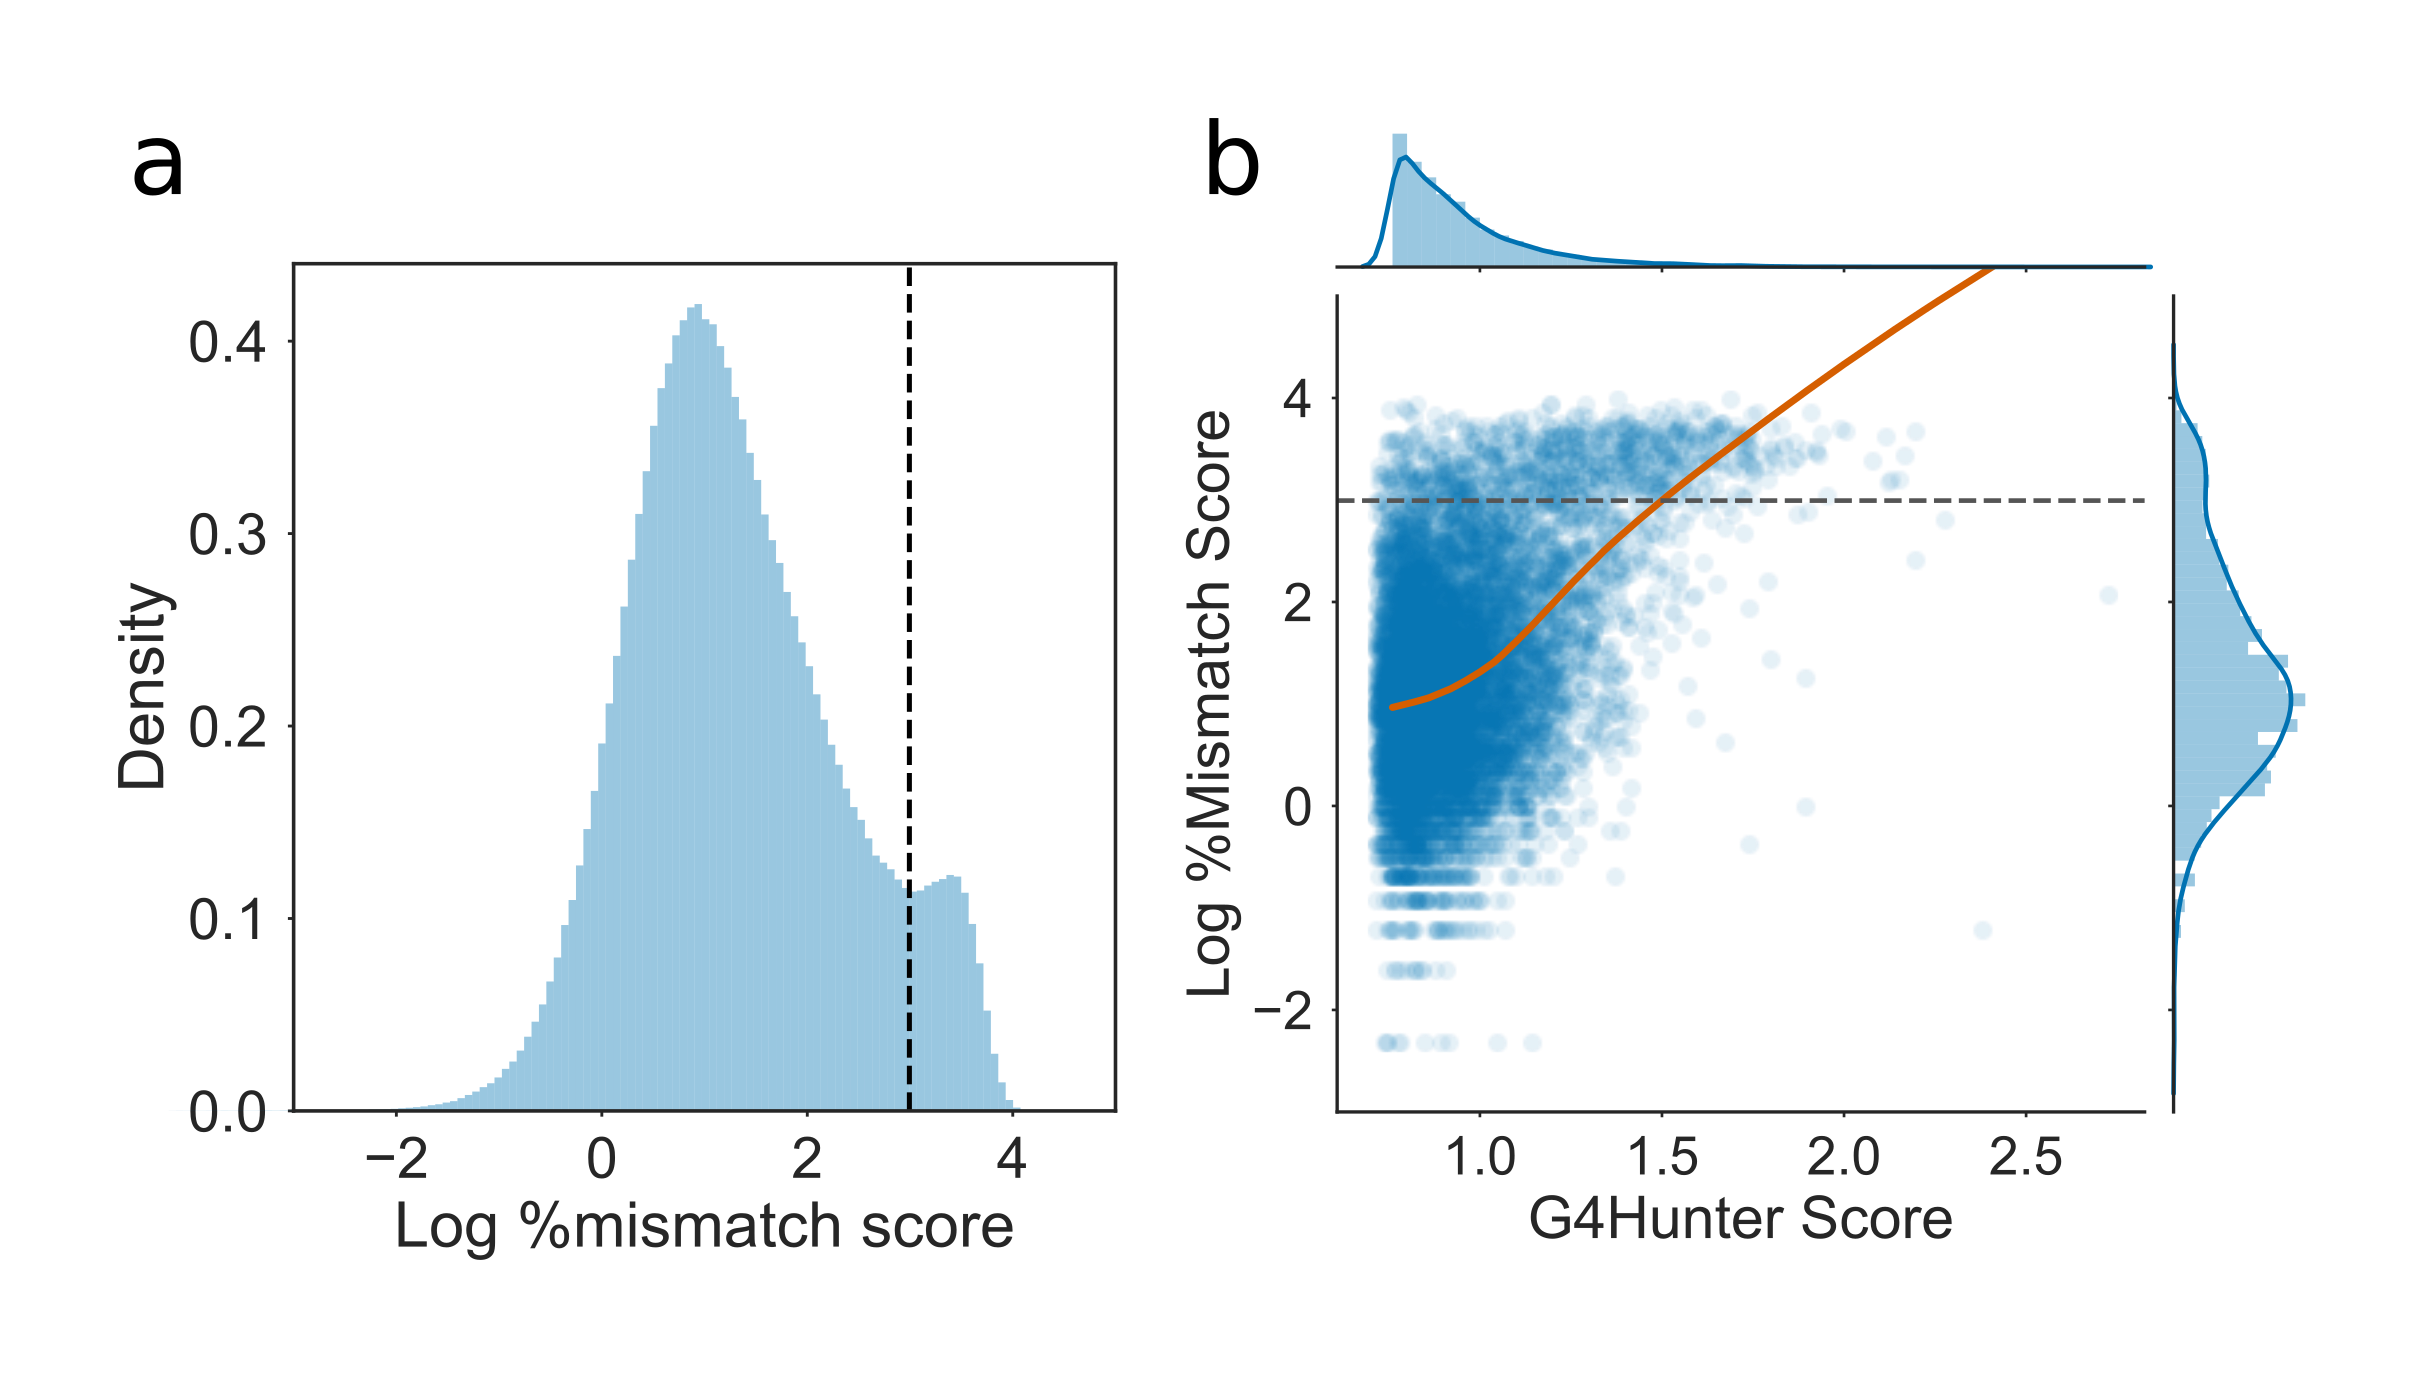
\includegraphics[width=\textwidth,height=562pt,keepaspectratio]{chapter_3/figures/training_data_dist.png}
\caption[Mismatch scores of candidate sequences identified by G4Hunter:]{\textbf{Mismatch   scores   of   candidate   sequences   identified   by   G4Hunter:}   \textbf{a)}   Histogram   of   log   percentage   mismatch   score   from   the   G4Seq   dataset,   for   the   50bp   sequences   identified   by   G4Hunter   (threshold   of   0.75).   Dashed   line   shows   the   threshold   chosen   to   delimit   G4   positive   and   G4   negative   sequences.   This   corresponded   to   around   20\%   mismatch   score.   \textbf{b)}   Joint   plot   of   log   mismatch   score   against   G4Hunter   score   for   10000   randomly   sampled   sequences.   Orange   line   shows   lowess   curve   fit.   \label{training_data}}
\end{figure}

\newpage

\hypertarget{model-selection-and-training}{%
\subsection{Model selection and
training}\label{model-selection-and-training}}

\label{ssec:results_model_choice}

Previously published G quadruplex prediction methods which utilise
machine learning techniques have used derived features such as
trinucleotide content to feed to models (Garant et al., 2017; Sahakyan
et al., 2017). These features result in the loss of some spatial
information about the sequence, however. For example, the sequence
\texttt{GGTGGTGGTGGGGGG} has the same trinucleotide composition as
\texttt{GGGTGGGTGGGTGGG}, but is unlikely to have equivalent G4 forming
propensity. Furthermore, Quadron derived features require input
sequences to conform to the QuadParser regular expression (Huppert and
Balasubramanian, 2005), meaning that Quadron is only able to improve the
precision of the QuadParser method, and not the recall. We opted for a
neural network involving convolutional layers (those often used for
image classification) that could make predictions directly from the
sequence itself, without any derived features whatsoever. This allows us
to make no assumptions about potential G4 patterns in the dataset.

The overall architecture selected was a convolutional-recurrent neural
network (Fig. \ref{architecture}), which has previously been used to
identify regulatory motifs in DNA (Quang and Xie, 2016). The first
layers of the architecture consists of two one dimensional convolutional
layers with a kernel size of 3. Convolutional layers contain a number of
separate filters which are convolved with the data to generate an output
function. The values (aka weights) in these filters are determined by
training. Each filter captures different local features in the sequence.
A maximum pooling layer then reduces the size of the output feature
space by half. These features are then fed to a bidirectional Long Short
Term Memory (LSTM) layer. LSTMs are recurrent layers, meaning that the
nodes of the layer form a linear directed graph over the input sequence.
The internal state of the node is dependent on the output from the
previous node, meaning that the model is able to ``remember'' features
it has previously seen in a sequence. LSTMs are therefore able to learn
and recognise long distance relationships between features in the
sequence.

The model outputs a single value between zero and one of the probability
of G4 formation. The dataset was split into three for training and
testing: 1,332,565 sequences (\textasciitilde{}80\%) were used for
training, 166,571 (\textasciitilde{}10\%) for in-training model
validation, and 166,576 (\textasciitilde{}10\%) for post-training model
testing.

\newpage

\begin{figure}[htbp]
\centering
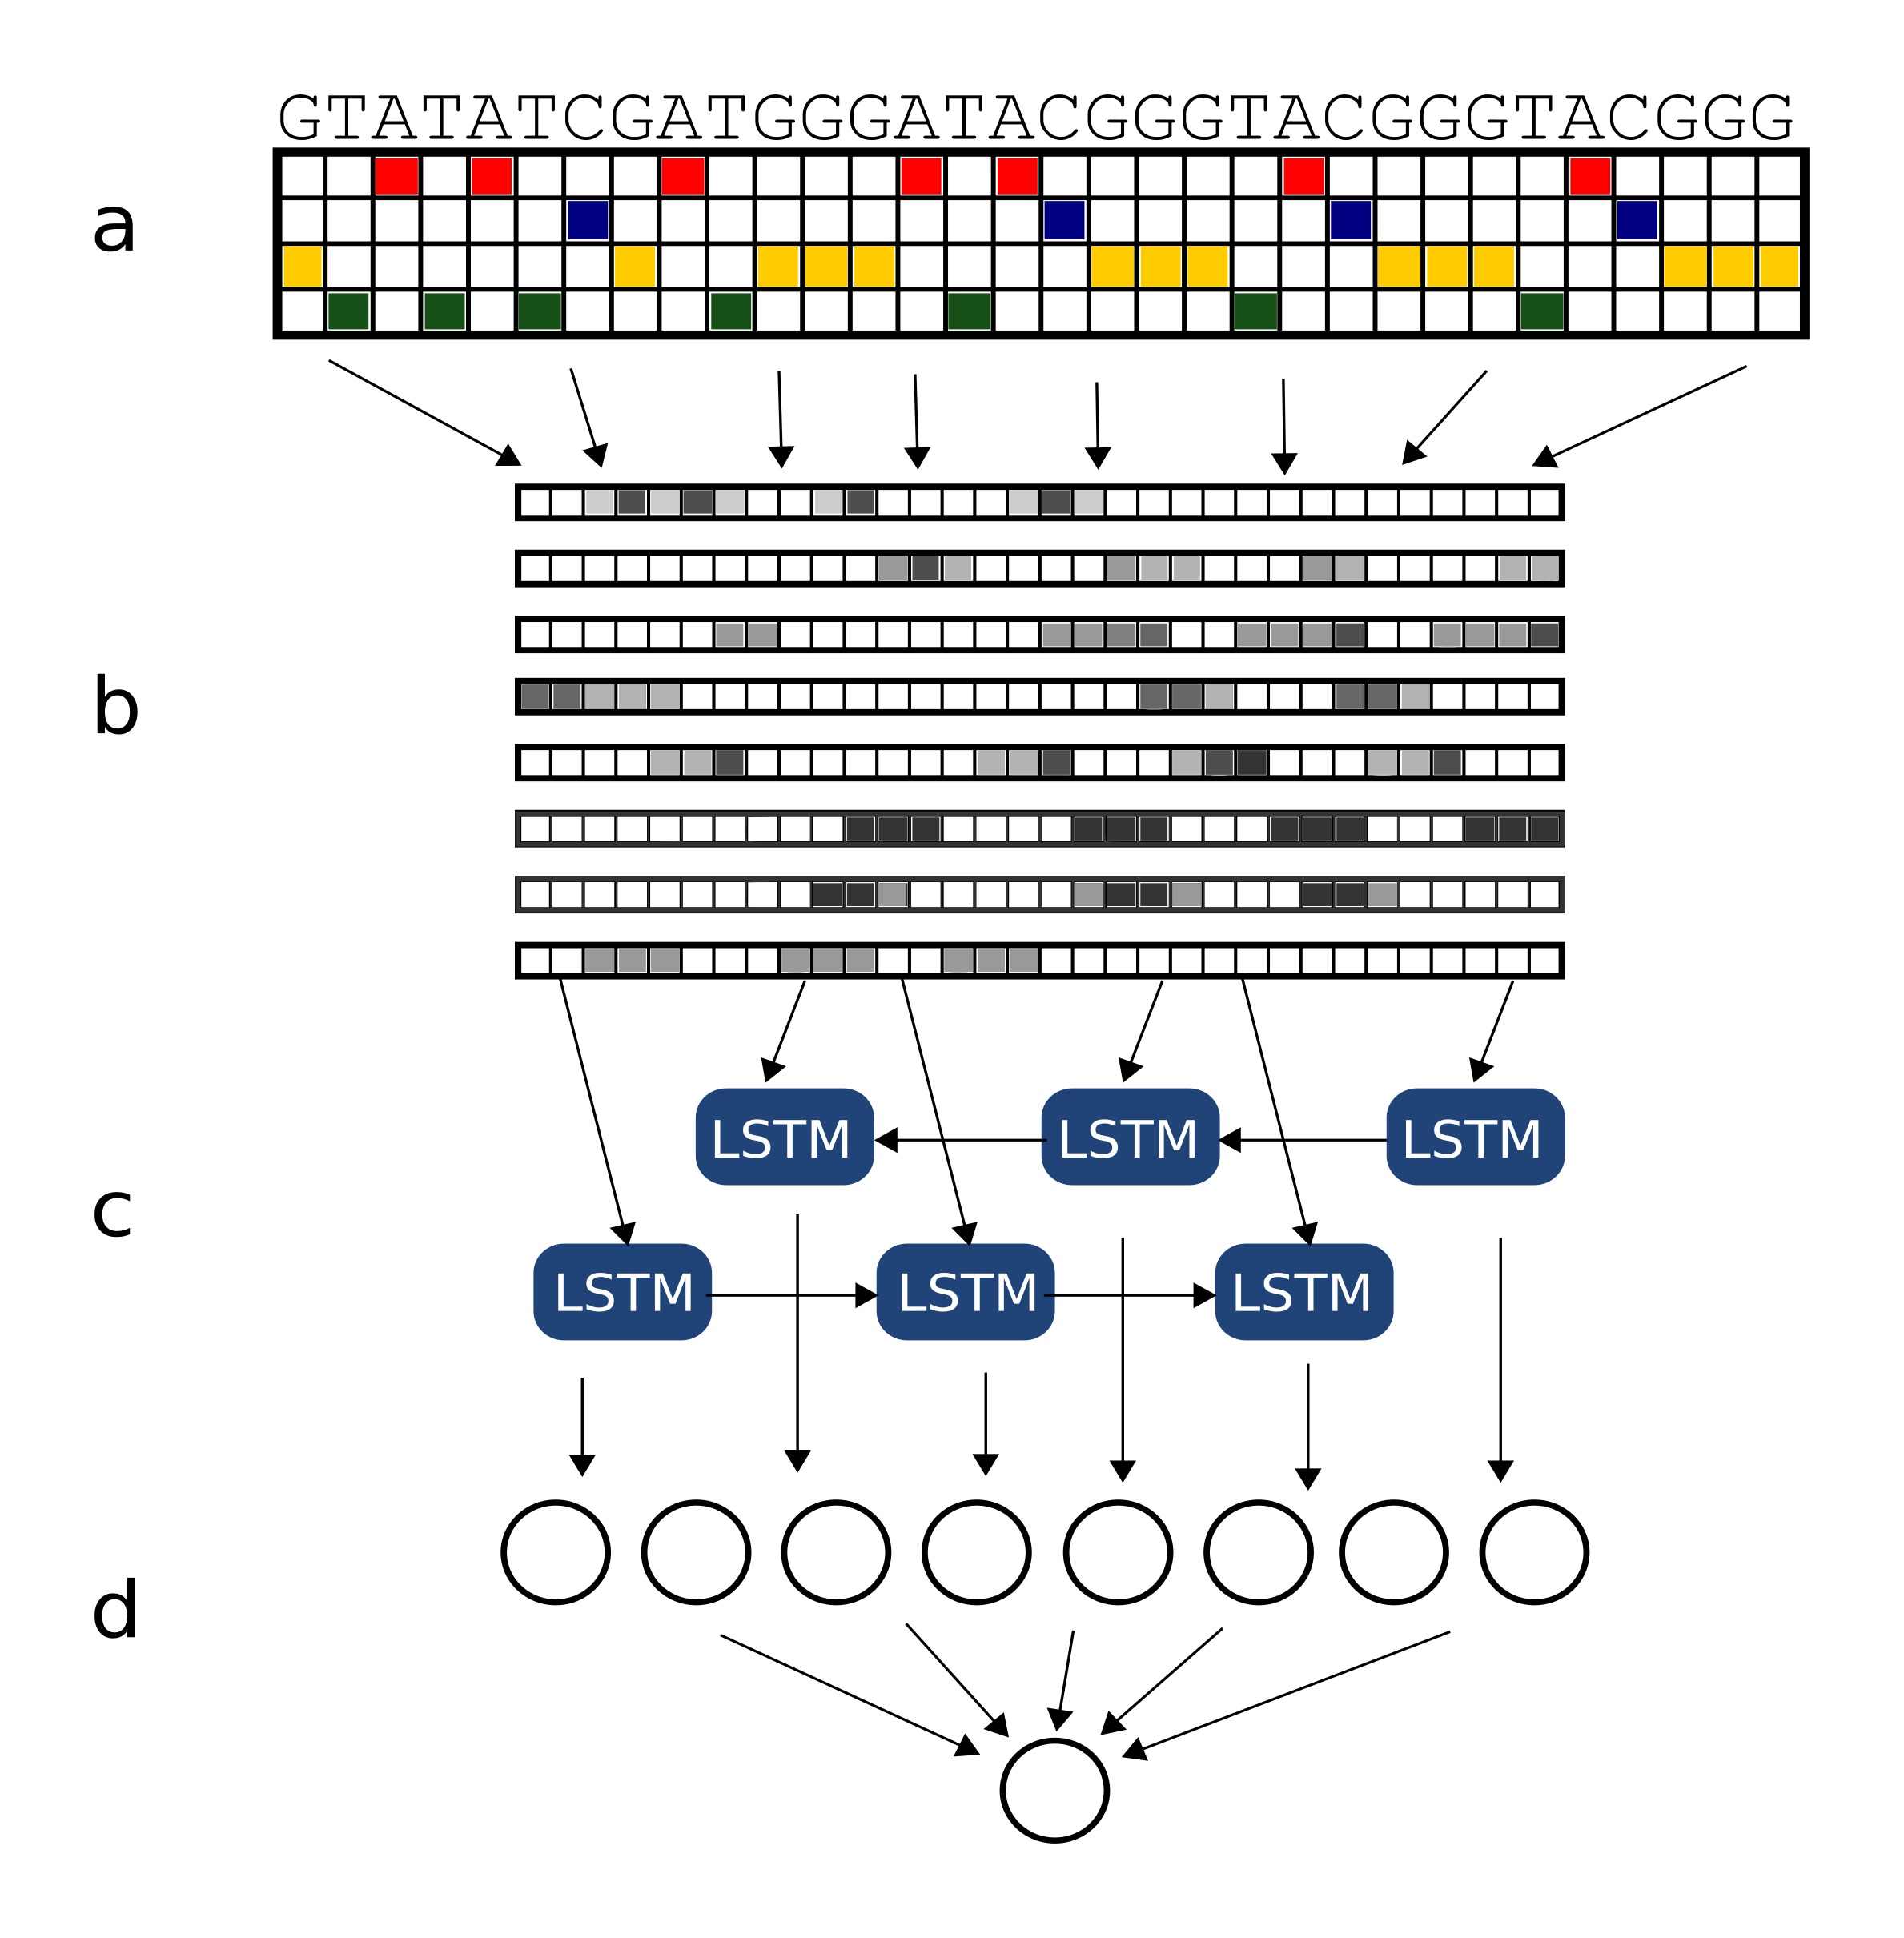
\includegraphics[width=\textwidth,height=562pt,keepaspectratio]{chapter_3/figures/architecture.png}
\caption[G4Seeqer architecture]{\textbf{G4Seeqer   architecture}   Adapted   from   Quang   \&   Xie   2016.   \textbf{a)}   Sequences   are   one   hot   encoded   to   produce   a   matrix   which   can   be   processed   by   the   neural   network.   \textbf{b)}   Input   matrices   are   passed   through   a   convolutional   layer.   Each   layer   contains   8   filters   which   are   trained   to   recognise   local   patterns   on   the   scale   of   3-6bp   in   size.   \textbf{c)}   Convolutional   features   are   passed   through   a   bidirectional   Long   Short   Term   Memory   (LSTM)   layer.   This   layer   recognises   long   distance   interactions   between   features   which   might   combine   to   produce   G4s.   \textbf{d)}   Finally,   features   are   passed   through   a   fully   connected   layer.   Output   from   the   model   is   a   single   probability   of   whether   the   sequence   forms   a   G4.   \label{architecture}}
\end{figure}

\newpage

\hypertarget{comparison-to-existing-methods}{%
\subsection{Comparison to existing
methods}\label{comparison-to-existing-methods}}

We benchmarked our technique (hereafter referred to as G4Seeqer) using
the 10\% of the data reserved for testing. The model was compared to our
modified G4Hunter method, as well as a multi-layer perceptron model
trained on trinucleotide frequencies derived from the same dataset as
was used to train G4Seeqer. This model allows us to compare the
methodology of G4RNA Screener (Garant et al., 2017) to our own method,
since G4RNA Screener was originally trained on a database of RNA G
Quadruplexes, and may not perform as well on a dataset derived from DNA.
The performance of the methods were calculated using the Receiver
Operating Characteristic area under curve (ROC AUC). We found that
neither G4Hunter (Bedrat et al., 2016) nor the G4RNA-like method
performed as well as G4Seeqer on the test dataset (AUC G4Hunter 0.82,
G4RNA Screener-like 0.90, G4Seeqer 0.94) (Fig. \ref{roc}a-b). This is
likely due to the loss of sequence spatial information in the former
methods.

To benchmark our method against the other G4Seq trained machine learning
G4 prediction package, Quadron, we downloaded and installed the Quadron
source code (Sahakyan et al., 2017). Quadron was used to score sequences
from the held out test set and compared to the performance of other
methods. Quadron requires larger flanking regions of 50bp, so test set
intervals and sequences were increased in length by 50bp in both
directions to produce test sequences of length 228. This was deemed the
best way to compare the two methods, however was still not ideal since
Quadron may have been trained on some or all of the test sequences.
Regions which had predictions associated with them by G4Hunter and
G4Seeqer but had no associated predictions from Quadron (due to not
conforming to the Quadparser regular expression) were given a Quadron
score of zero. The ROC curve of Quadron (AUC 0.7) ((Fig. \ref{roc}a-b))
had interesting properties: the model is capable of producing a true
positive rate of around 30\% with a false positive rate of less than
1\%, however shortly beyond this point in the ROC curve the curve
becomes linear. This is because Quadron is only capable of scoring
sequences which conform to the Quadparser method, with all other
sequences being scored zero. Since these sequences only account for a
25\% of all the potential PG4 forming sequences in the test set, the
model does not perform well on the full dataset. Because it makes no
assumptions about the input sequence, G4Seeqer is able to make accurate
predictions for all forms of PG4 in the test data, as reflected in the
ROC curve.

We were interested in how G4Seeqer compared against Quadron on only
sequences which conformed to the Quadparser motif. We therefore filtered
our dataset for intervals on which Quadron had made a prediction, and
replotted the ROC curves and Precision Recall curves for the filtered
data (Fig. \ref{roc}c-d). As expected the AUC for Quadron was much
better on this filtered set (AUC 0.93), however it was still
outperformed by G4Seeqer (AUC 0.94), suggesting that G4Seeqer captures
the same or more explanatory information directly from the input
sequence.

\newpage

\begin{figure}[htbp]
\centering
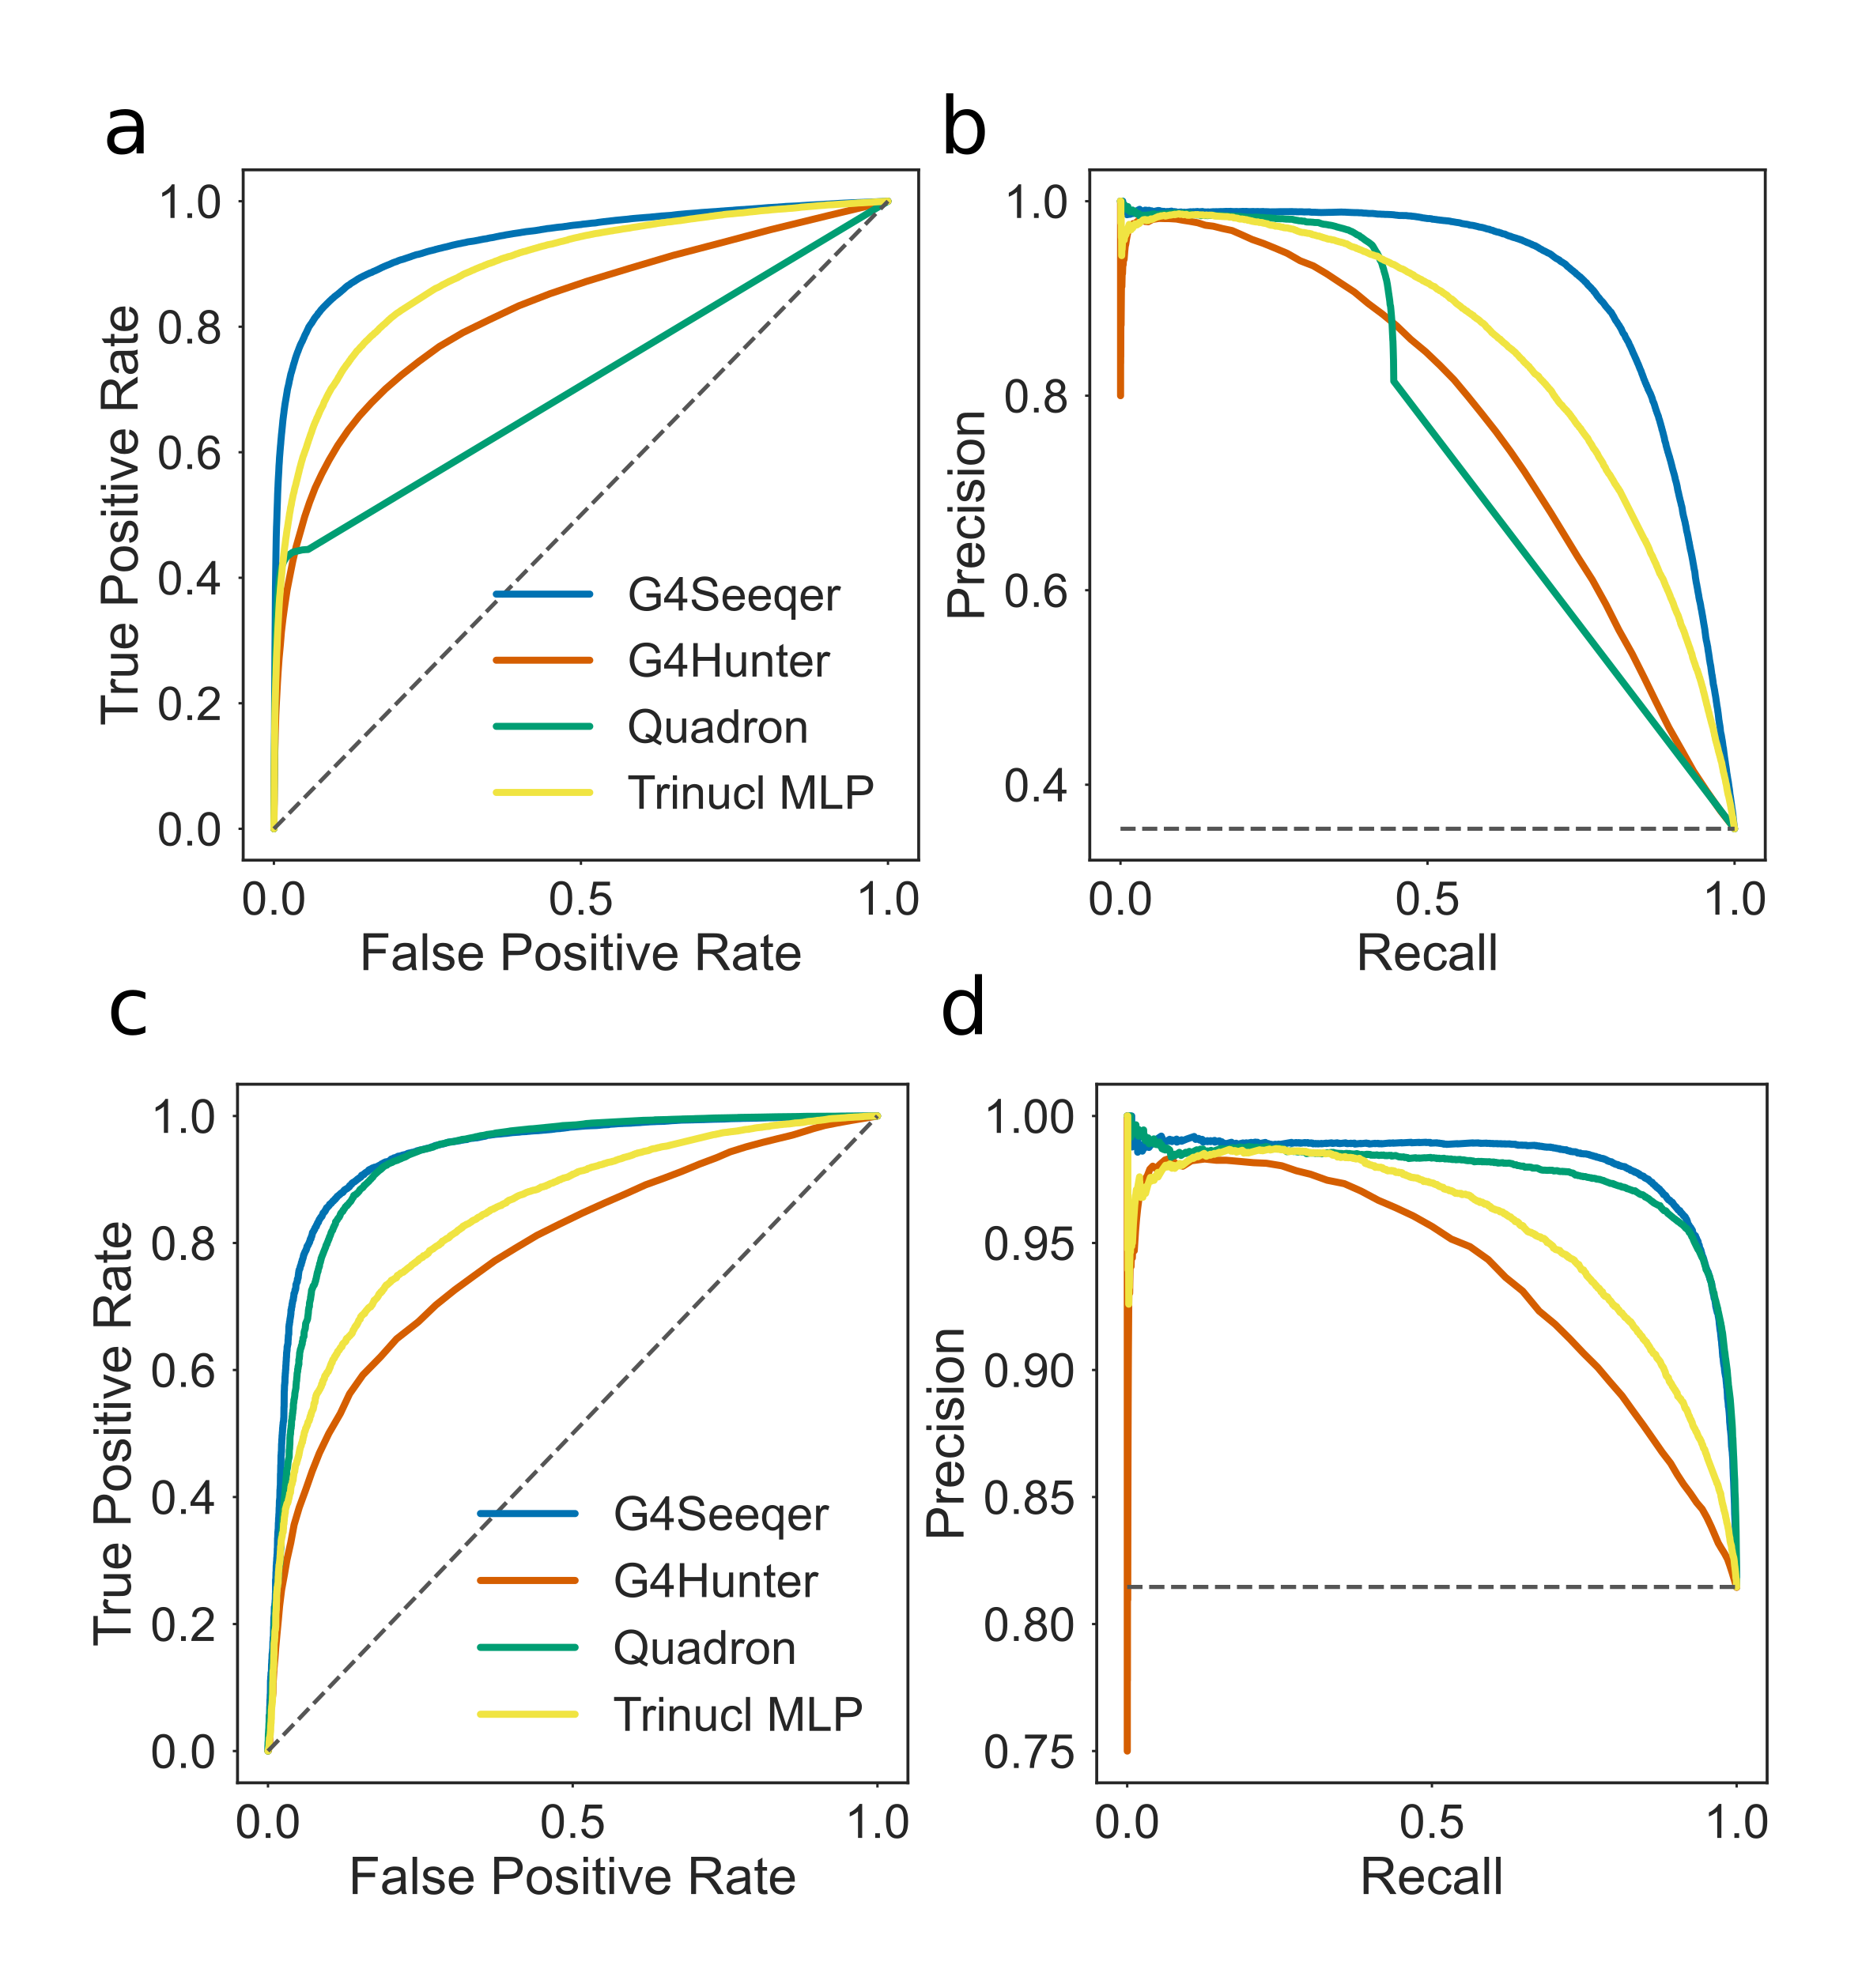
\includegraphics[width=\textwidth,height=562pt,keepaspectratio]{chapter_3/figures/test_set_roc_pr.png}
\caption[Validation curves for G4Seeqer method]{\textbf{Validation   curves   for   G4Seeqer   method}   \textbf{a)}   Receiver   Operator   Characteristic   (ROC)   curve   showing   the   performance   of   G4Seeqer,   Multi-Layer   Perceptron   (MLP)   trained   on   trinucleotide   contents,   Quadron,   a   Gradient   Boosted   Machine   model   (Sahakyan   et   al. 2017)   and   the   G4Hunter   method   (Bedrat   et   al. 2016),   on   a   held   out   test   set   of   the   G4Seq   dataset   (10\%   of   total   dataset).   \textbf{b)}   Precision-recall   curves   showing   the   performance   of   G4Seeqer,   trinucleotide   MLP,   Quadron,   and   G4Hunter   on   the   same   dataset.   \textbf{c)}   ROC   curve   and   \textbf{d)}   Precision   Recall   curve   showing   the   performance   on   sequences   from   the   test   set   conforming   to   the   Quadparser   motif.   \label{roc}}
\end{figure}

\newpage

\hypertarget{bg4-chip-seq-data-evaluation}{%
\subsection{BG4 ChIP-seq data
evaluation}\label{bg4-chip-seq-data-evaluation}}

Further model validation was performed on G4s experimentally validated
by an entirely different technique, namely G4-chromatin
immunoprecipitation (BG4) (Hänsel-Hertsch et al., 2016). The BG4 dataset
is arguably more biologically relevant than G4seq since G4 structures
are not induced by addition of potassium, and are captured from native
chromatin. BG4 peak intervals were shuffled to produce a set of G4
negative sequences, and then the performance of the models was evaluated
on the real and shuffled peaks. For each BG4 interval, the highest
scoring overlapping prediction for each model was assigned. Any
intervals with no overlapping predictions were scored zero for that
model. We tested the G4Seeqer, G4Hunter and Quadron methods. As with the
G4Seq test dataset, we found that Quadron performed reasonably for
Quadparser conforming BG4 peaks, but was unable to identify most of the
true positive BG4 peaks due to its restriction to the pattern. G4Seeqer
performed better on all BG4 peaks, with an AUC of 0.71, however was only
marginally better than the G4Hunter technique (AUC 0.7) (Fig.
\ref{bg4}). These results suggest that the information within the G4Seq
dataset, when captured by a suitable model, is predictive of G4s in an
\emph{in vivo} setting.

\newpage

\begin{figure}[htbp]
\centering
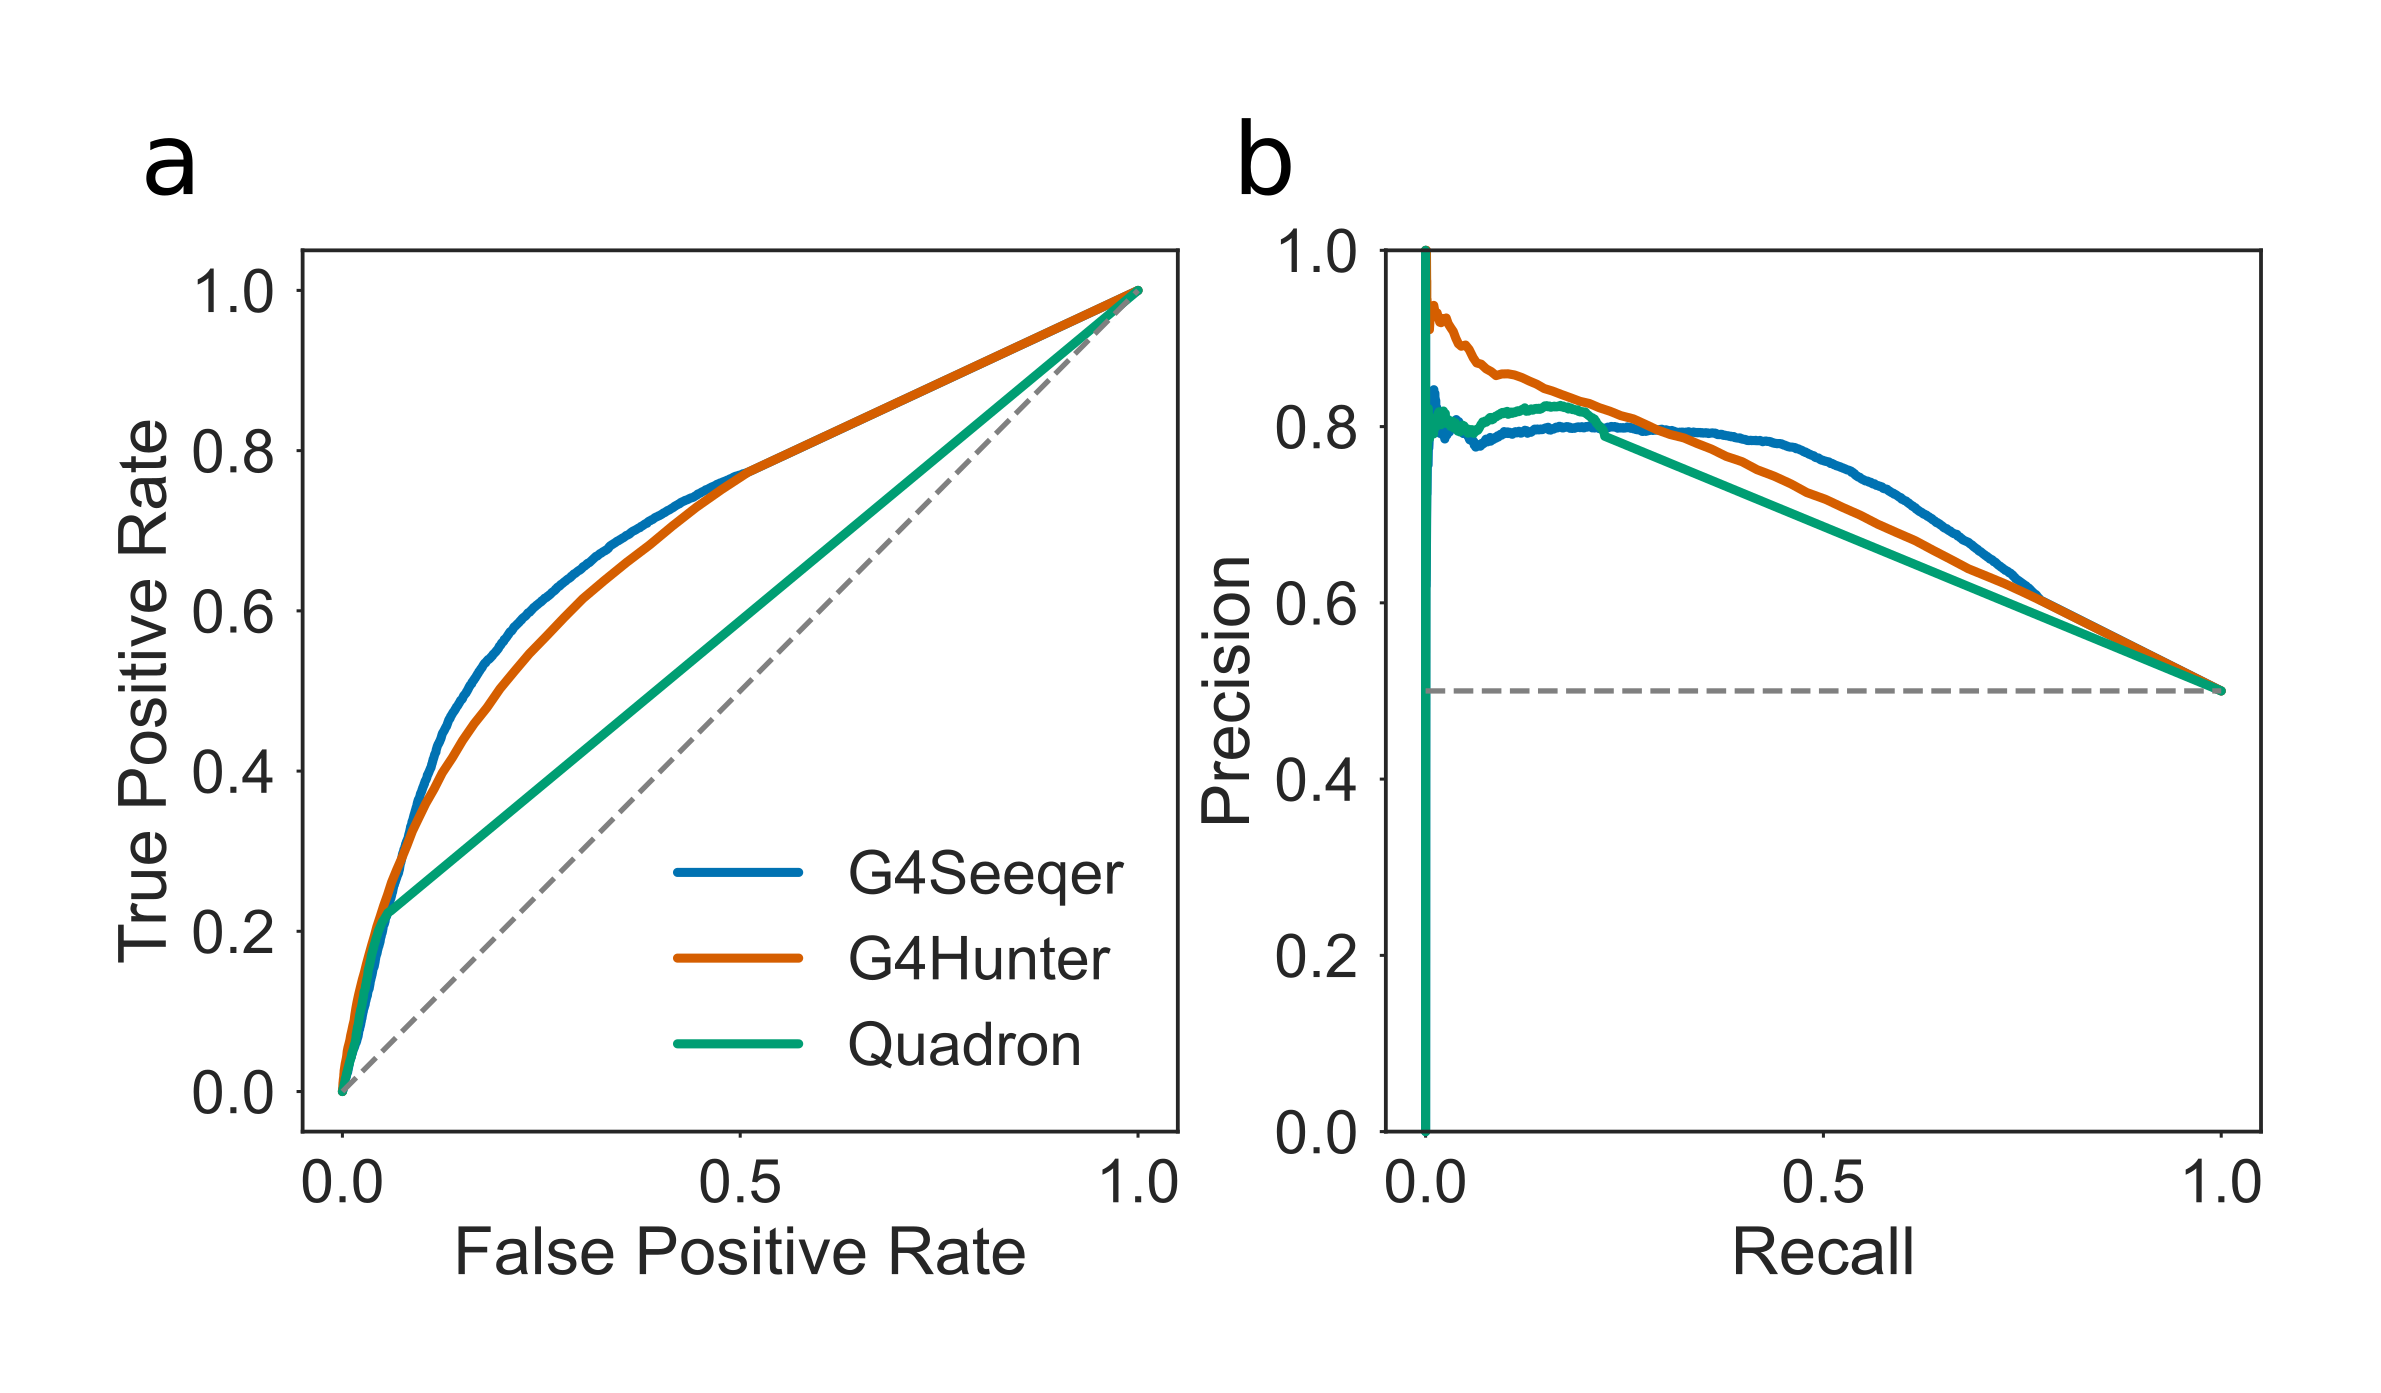
\includegraphics[width=\textwidth,height=562pt,keepaspectratio]{chapter_3/figures/bg4_roc.png}
\caption[Detection by BG4 peak sequences using G4Seeqer]{\textbf{Detection   by   BG4   peak   sequences   using   G4Seeqer}   \textbf{a)}   Receiver   Operator   Characteristic   (ROC)   curve   showing   the   performance   of   G4Seeqer,   Quadron,   and   the   G4Hunter   method,   on   BG4   ChIP-seq   peaks   and   randomly   shuffled   negative   sequences.   \label{bg4}}
\end{figure}

\newpage

\hypertarget{transfer-learning-on-rna-g4seq-rg4seq-dataset}{%
\subsection{Transfer learning on RNA G4Seq (rG4seq)
Dataset}\label{transfer-learning-on-rna-g4seq-rg4seq-dataset}}

PG4s with the same sequence are likely to have slightly different G4
forming potentials in DNA and RNA, due to the chemical differences in
these molecules. The sugars which make up the backbone of RNA are
riboses, which have an extra 2' hydroxyl group compared to the
deoxyribose found in DNA. This extra hydroxyl group is thought to have a
number of implications for G4 formation: it increases the number of
backbone hydrogen bonds in the G4, increasing its enthalpic
favourability and its entropic favourability (by reducing the number of
coordinated water molecules) (Collie et al., 2010). Furthermore, the 2'
hydroxyl introduces steric constraints which make parallel RNA G4s much
more favourable than anti-parallel ones (Collie et al., 2010). Given
these differences, it is likely therefore that a model specifically
trained on DNA G4 sequences will not perform optimally on RNA G4s.

To address this issue, we decided to retrain G4Seeqer using the rG4seq
dataset produced by Kwok et al.~2016, to create an rG4Seeqer model (Kwok
et al., 2016). Data was prepared similarly to the data for G4Seeqer:
candidate regions were selected from human exonic sequences using
G4hunter with window size of 50bp and a threshold of 0.75. This yielded
a set of 186279 putative RNA G4 forming sequences, which were increased
by 39bp in each direction to get flanking sequences. These were then
intersected with rG4seq hits collected under potassium stabilising
conditions (Kwok et al.~2016). Of the 3383 identified RNA G4s in the
rG4seq dataset, 2811 (83\%) overlapped with G4hunter windows. rG4seq
negative examples were undersampled with a ratio of 2:1 to yield 7518
training samples. 80\% of these were used for training, with 10\% for
validation and 10\% held out for testing.

Because of the significantly smaller size of the rG4seq derived training
set, we found that the method for training which yielded most optimal
results was transfer learning from the G4Seeqer model. Weights of the
initial convolutional feature extraction layers were therefore held
constant, and only the weights of the LSTM layers (which find long range
interactions) and dense output layers were retrained.

Testing was first conducted on the held out set of 752 sequences using
G4Hunter, G4Seeqer and the newly trained rG4Seeqer. G4Seeqer
significantly outperformed G4Hunter (AUC 0.9 vs 0.83 respectively),
suggesting that the information extracted from the G4Seq dataset is
applicable to the rG4seq dataset (Figure \ref{rG4seeqer_test}).
rG4Seeqer outperformed both methods, however (AUC 0.95), demonstrating
that domain specific information is better for predicting RNA G4s in the
rG4seq dataset (Figure \ref{rG4seeqer_test}).

\newpage

\begin{figure}[htbp]
\centering
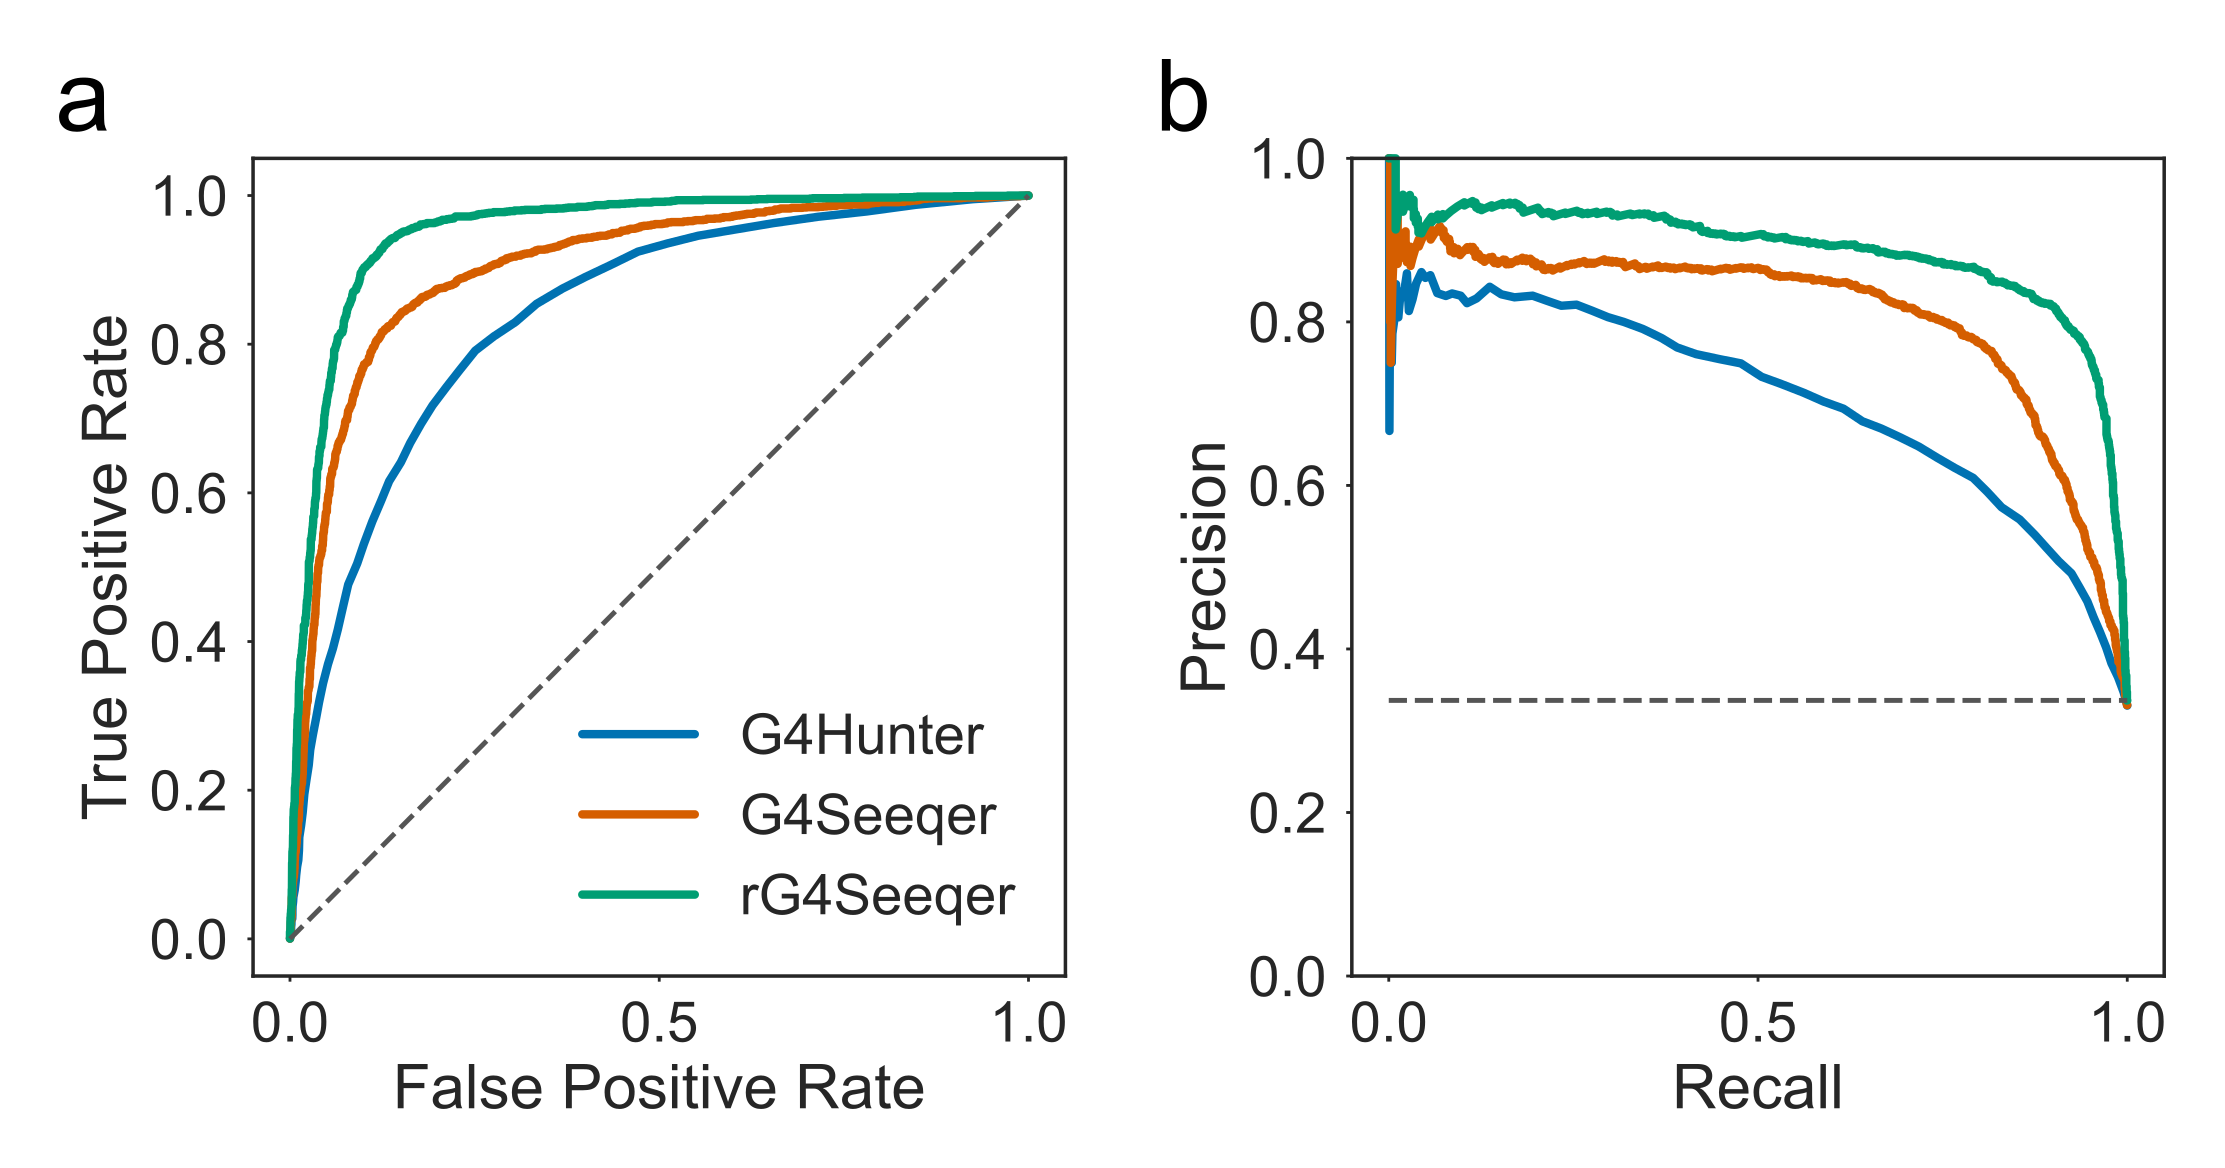
\includegraphics[width=\textwidth,height=562pt,keepaspectratio]{chapter_3/figures/rg4seq_test_set_roc_pr.png}
\caption[Validation curves for rG4Seeqer method]{\textbf{Validation   curves   for   rG4Seeqer   method}   \textbf{a)}   Receiver   Operator   Characteristic   (ROC)   curves   showing   the   performance   of   rG4Seeqer,   G4Seeqer   and   the   G4Hunter   method   (Bedrat   et   al. 2016),   on   a   held   out   test   set   of   the   rG4Seq   dataset   (10\%   of   total   dataset).   \textbf{b)}   Precision-recall   curves   showing   the   performance   of   rG4Seeqer,   G4Seeqer,   and   G4Hunter   on   the   same   dataset.   \label{rG4seeqer_test}}
\end{figure}

\newpage

We sought to test rG4Seeqer on G4s identified by a variety of physical
methods, using the set of RNA G4s curated by Garant et al.~for their
model, G4RNA Screener (Garant et al., 2017). We used 347 sequences from
this dataset, of which 169 sequences were G4 positive and 178 were G4
negative. G4Seeqer and rG4Seeqer predictions were calculated by padding
with random sequences to a length of 128bp before one hot encoding. This
was conducted 1000 times for each sequence and the mean score was taken.
G4RNA screener scores were taken directly from the supplemental
information of Garant et al.~2017. G4RNA screener was found to perform
best on the dataset (AUC 0.91), perhaps unsurprisingly since it was
trained directly on the sequences. Perhaps more importantly, rG4Seeqer
significantly outperformed G4Seeqer on the dataset (AUC 0.89 vs 0.82),
showing that the rG4seq trained model generalises better to RNA G4
sequences than the G4seq trained model.

\newpage

\begin{figure}[htbp]
\centering
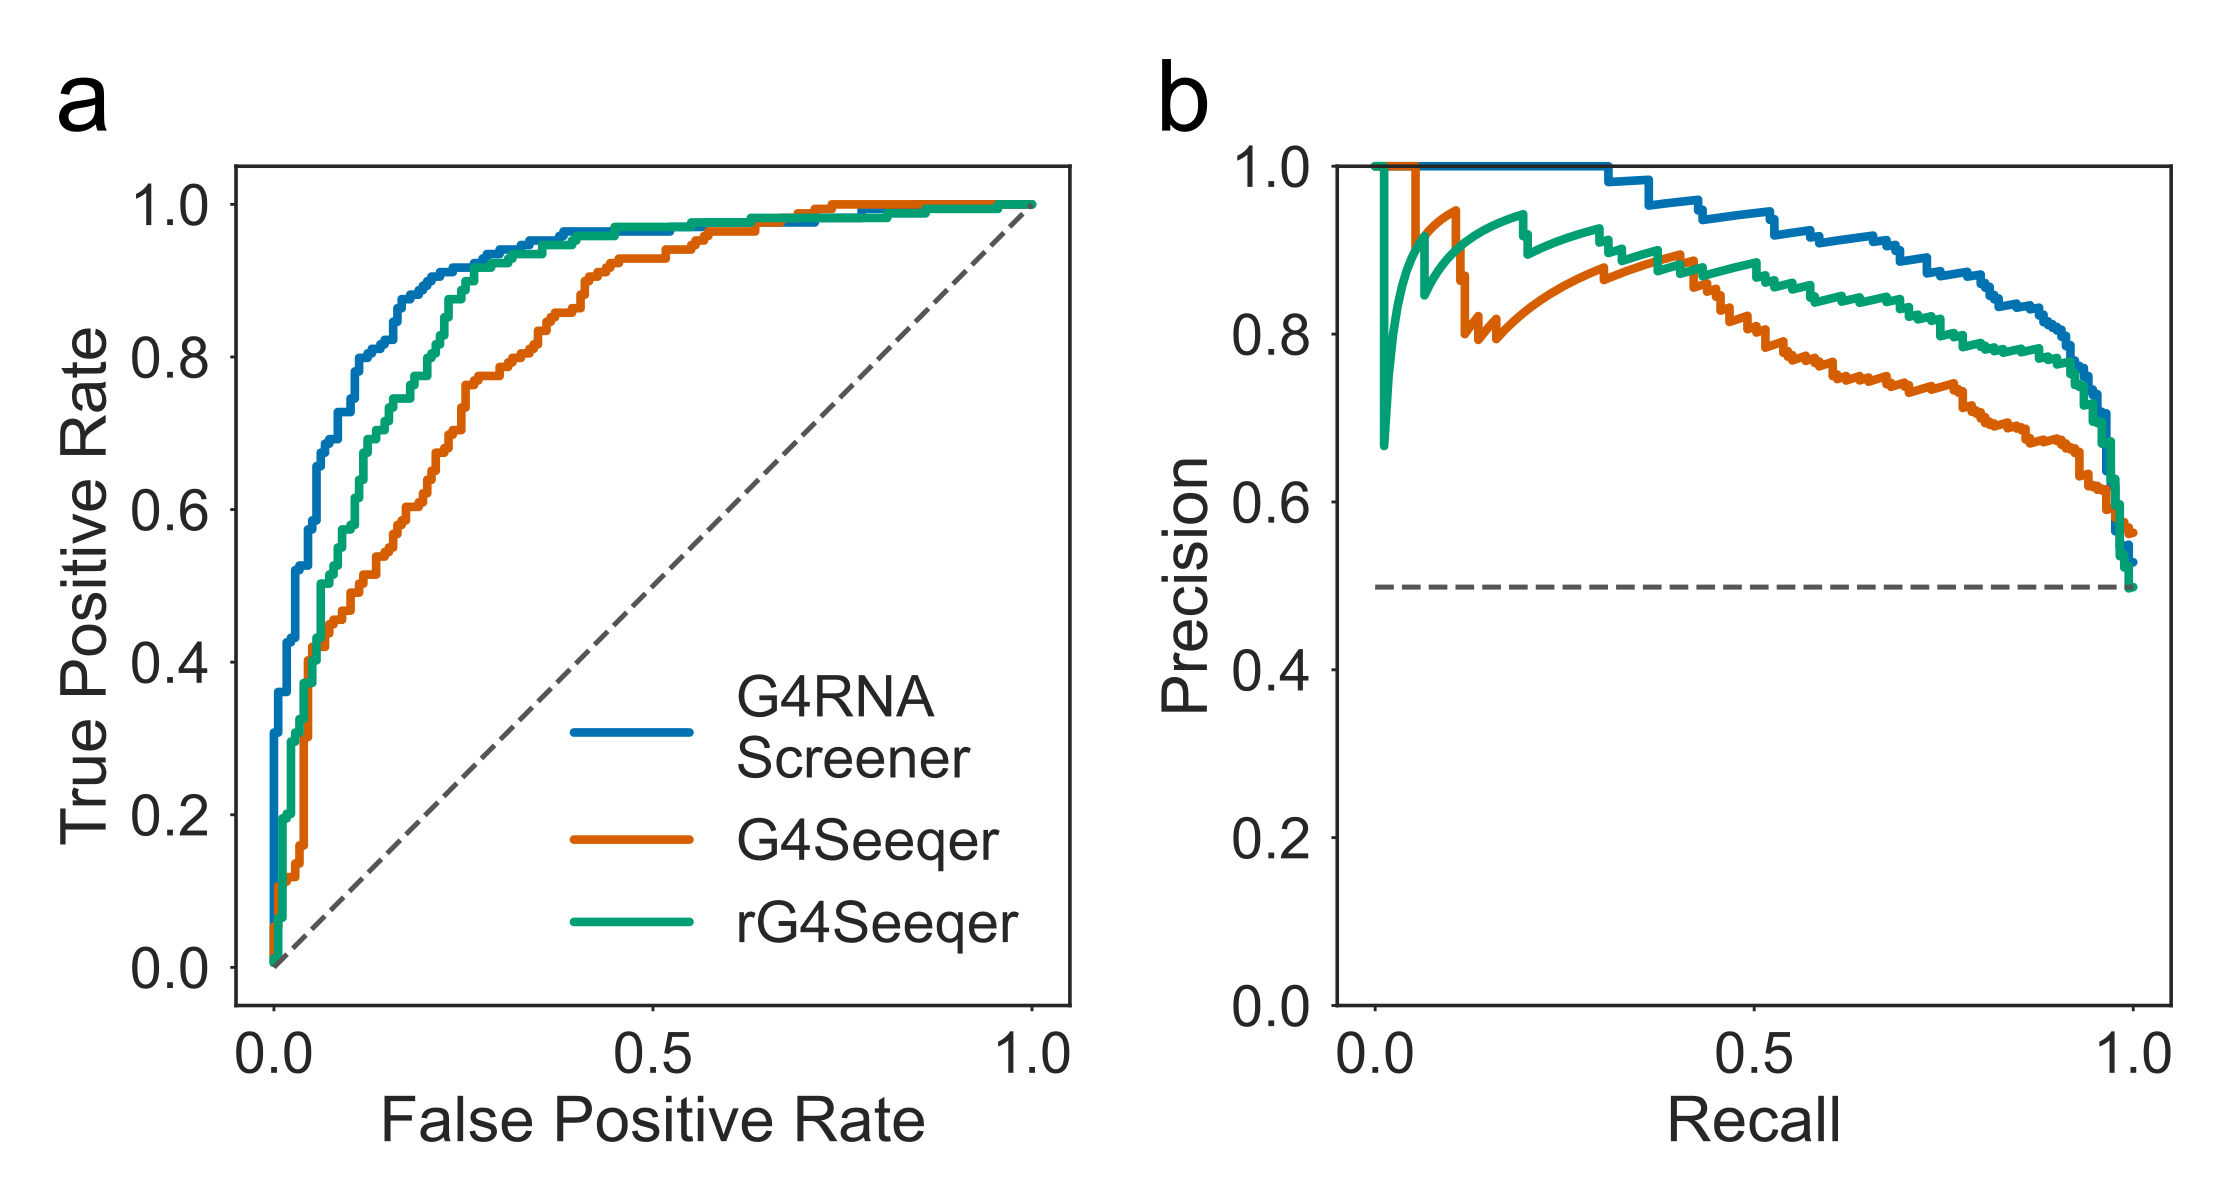
\includegraphics[width=\textwidth,height=562pt,keepaspectratio]{chapter_3/figures/g4rna_roc_pr.png}
\caption[Validation of rG4Seeqer on \textit{in vitro} experimentally categorised RNA sequences]{\textbf{Validation   of   rG4Seeqer   on   \textit{in   vitro}   experimentally   categorised   RNA   sequences}   \textbf{a)}   Receiver   Operator   Characteristic   (ROC)   curves   showing   the   performance   of   rG4Seeqer,   G4Seeqer   and   the   G4RNA   Screener   method   (Garant   et   al. 2017),   on   the   G4RNA   dataset   curated   by   Garant   et   al.   \textbf{b)}   Precision-recall   curves   showing   the   performance   of   rG4Seeqer,   G4Seeqer,   and   G4RNA   Screener   on   the   same   dataset.   \label{rG4seeqer_test}}
\end{figure}

\newpage

\hypertarget{interpreting-g4seeqer-output-using-mutation-mapping}{%
\subsection{Interpreting G4Seeqer output using Mutation
Mapping}\label{interpreting-g4seeqer-output-using-mutation-mapping}}

One common complaint about neural network techniques is that the
complexity of the models they produce make them ``black boxes'' which
are impossible for humans to understand or extract useful knowledge or
rules from. It is possible, however, to visualise some of the output of
a neural network through various means. One commonly used method for
interpretation is the ``saliency'' of the network, which can produce
heatmaps showing the attention of the network to specific regions of the
input image or sequence. This can be used to determine the important
aspects of the input in classification. For biological sequences,
previous studies have used similar methods, called ``Mutation Maps'', to
analyse the importance of individual nucleotide positions on
convolutional neural network model predictions (Alipanahi et al., 2015;
Quang and Xie, 2016). Simply, the importance of each particular
nucleotide is evaluated by replacing it with each of the other three
bases, and calculating the change in model score. This is then used to
build a heatmap which can be used to visualise the importance of each
position.

Previous studies have highlighted a possible role for G4 forming
sequences in promoters, with G4 formation tending to have a positive
effect on expression, particularly in proto-oncogenes (Eddy and Maizels,
2006; Hänsel-Hertsch et al., 2016). We therefore decided to use the
mutation map approach to characterise PG4s in promoter regions extracted
from the ENSEMBL regulatory build (Zerbino et al., 2015). Promoter
sequences were screened using G4Seeqer and single base mutation maps
were created for each candidate PG4, including those regions where the
neural network score was low. Unsurprisingly, all of the most
deleterious single base substitutions (causing a score reduction of more
than 0.9) predicted by G4Seeqer mutation mapping were G-\textgreater{}H
changes.

We identified PG4 sequences scoring more than 0.9 for which a single
G-\textgreater{}H change resulted in a reduction of as much as 0.9 in
score (i.e.~switched the score from strongly PG4 positive to strongly
PG4 negative) (Fig. \ref{triplex}a). Analysis of the mutation maps for
these sequences showed that the majority of contained regions containing
three G-runs with short connecting loops. These tended to have a long
final loop to the next homopolymeric G-run, or no final G-run within the
window size. Any G-\textgreater{}H mutation in these G-dense regions
strongly affected the predicted G4 forming ability. Recent work by Hou
et al.~has shown that formation of G4 structures in human telomeric
sequences occurs via a stable G-triplex structure (Hou et al., 2017). We
believe these results suggest that the G4seq dataset is either capturing
mismatches caused by G-triplex structures, or by G-quadruplexes formed
from short range G-triplex interaction with more long range single
G-runs. To further illustrate this we predicted all short looped (1-4bp)
G-triplexes in the human genome which did not overlap with a Quadparser
predicted PG4 (loop lengths 1-12bp). We found that 35\% of these were
associated with a \%mm score greater than 20\%, suggesting the formation
of some secondary structure (Fig. \ref{triplex}b). To see if medium
range G-run interactions might stabilise these, we then measured, for
each G-triplex, the distance to the next run of at least three Gs on the
same strand, and compared this to the \%mm score. We found a weak
negative correlation between distance and \%mm score (Spearmans rho
-0.2) for G triplexes with a G-run less than 100bp away, suggesting that
these longer range interactions do occur but become weaker with distance
(Fig. \ref{triplex}c). This could be due to a reduction in G4 stability
with loop length, but could equally be explained by a reduction in the
likelihood of the next G-run being contained in the same sequenced
fragment. No clear difference was observed in the correlation of \%mm
score with upstream or downstream G-runs (Spearmans rho -0.17 and -0.15
respectively) suggesting there is no preference for the long loop region
to be at the 5' or 3' of the G triplex.

\newpage

\begin{figure}[htbp]
\centering
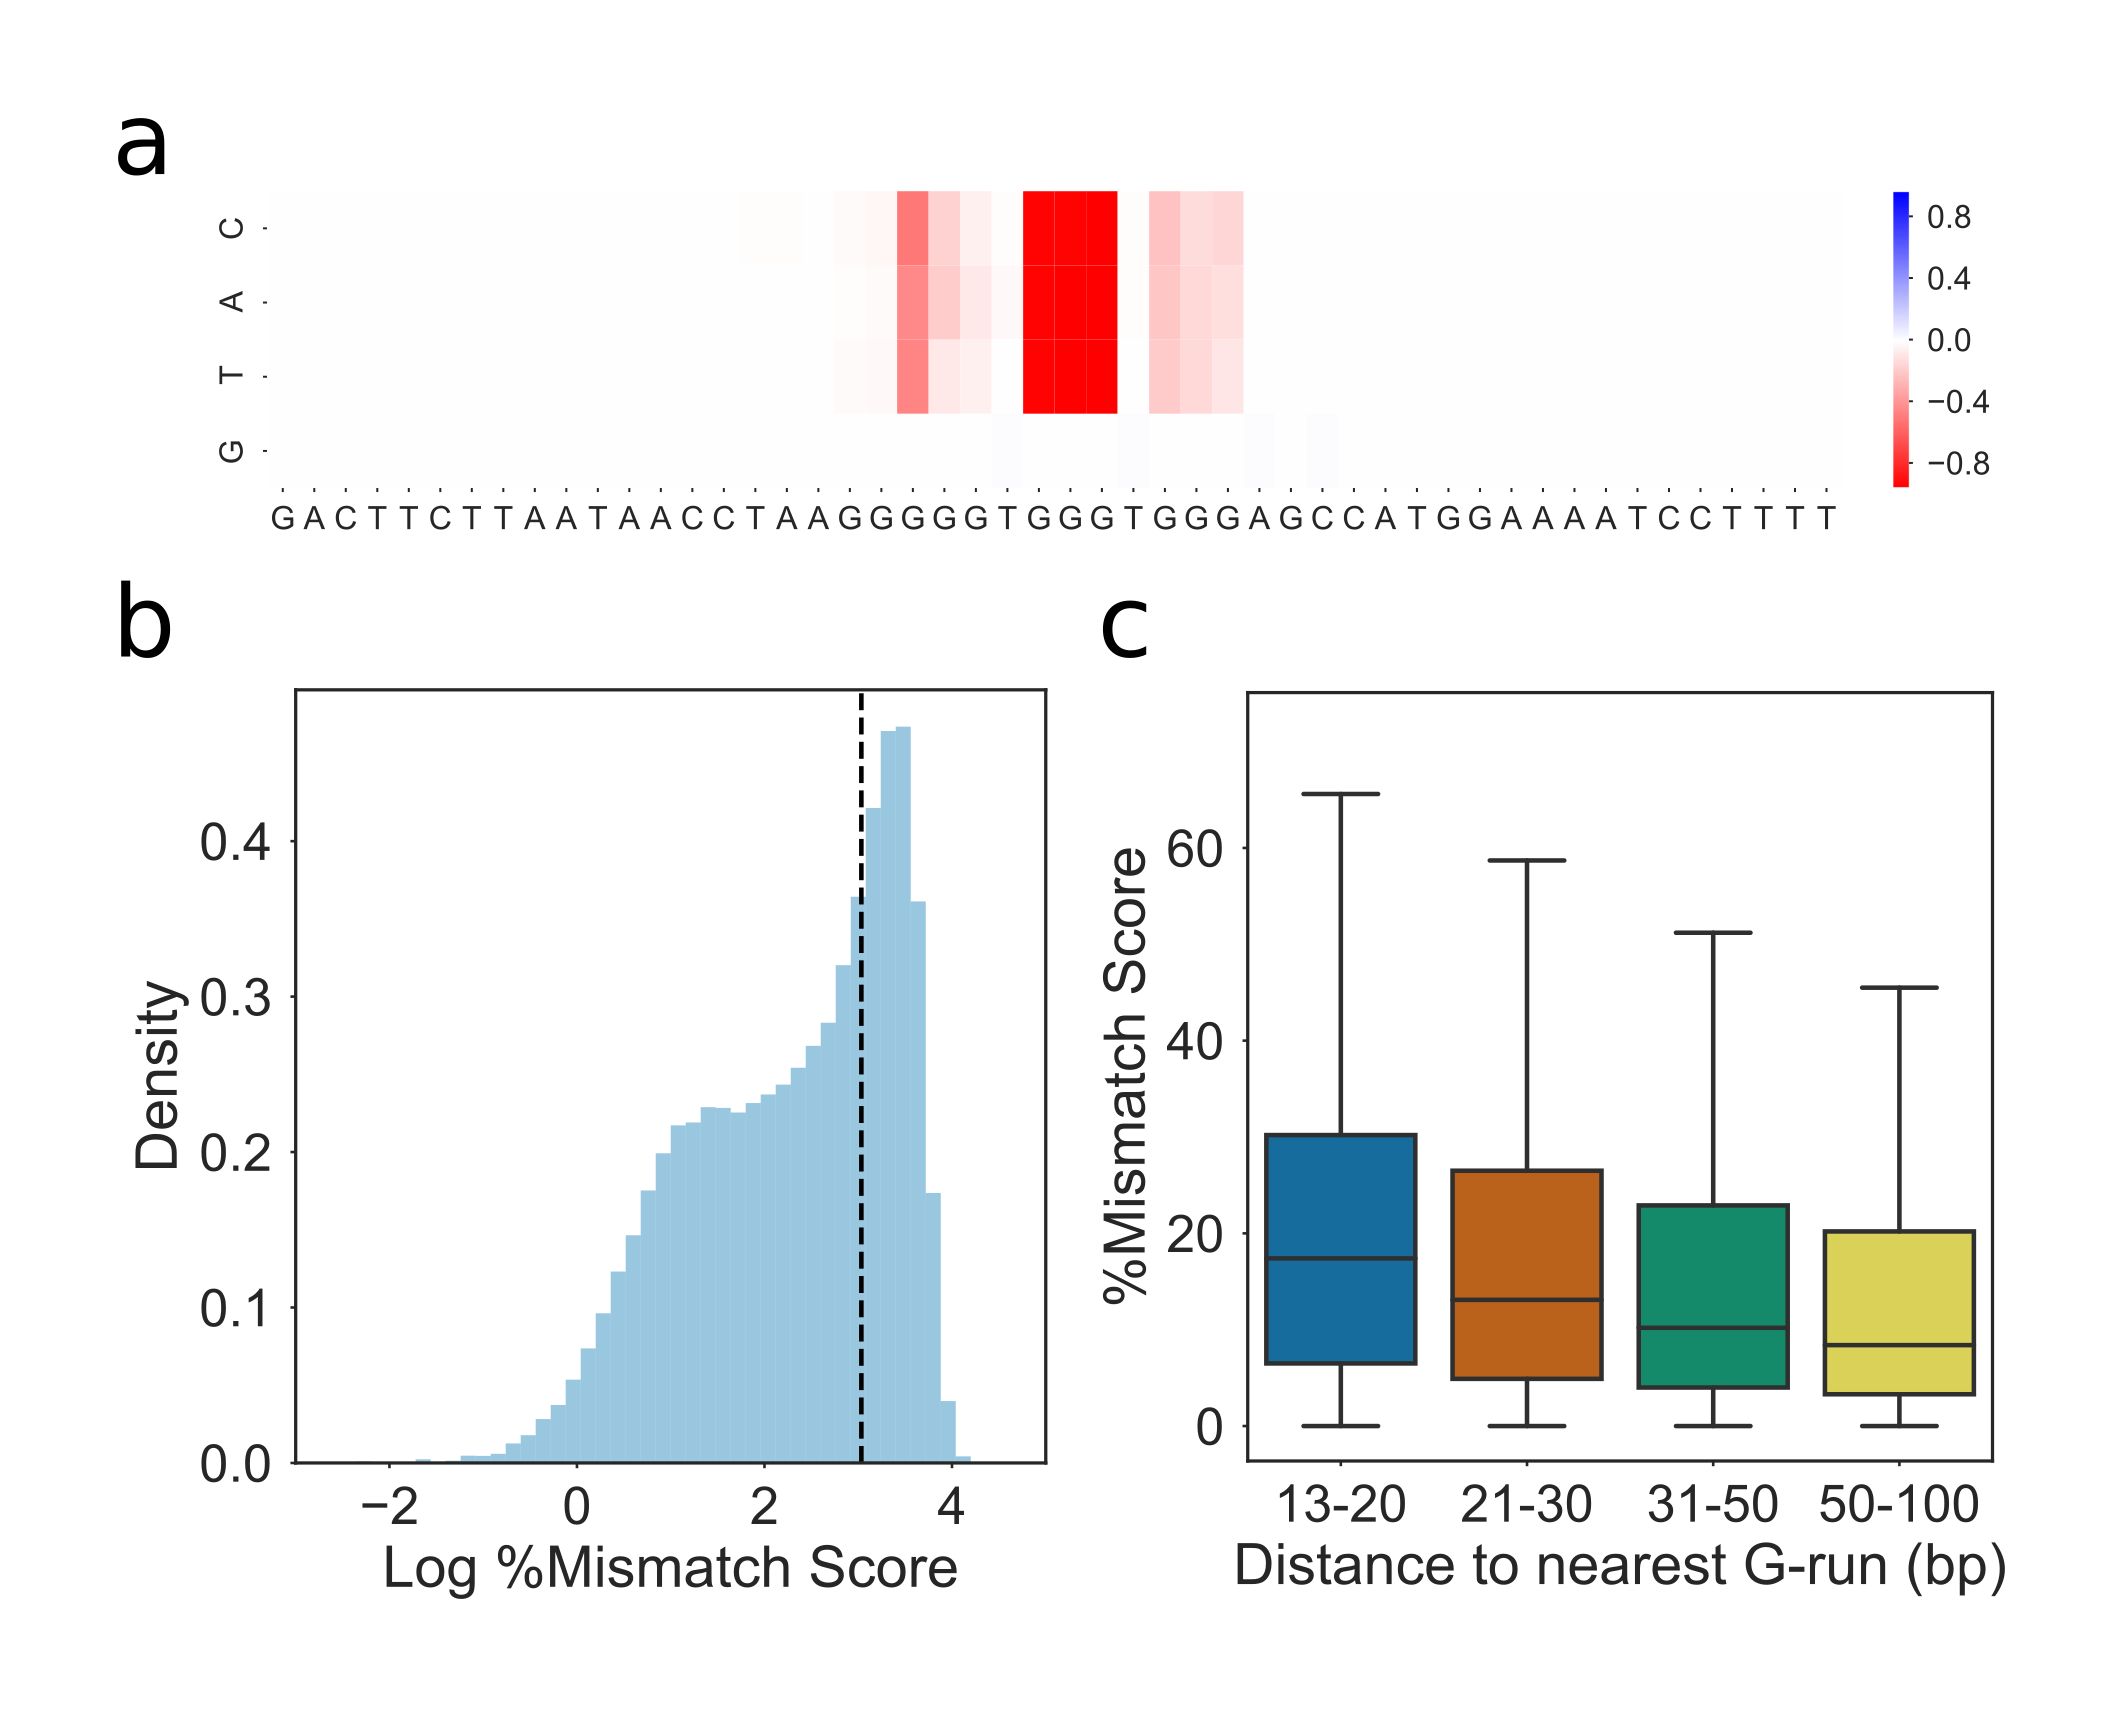
\includegraphics[width=\textwidth,height=562pt,keepaspectratio]{chapter_3/figures/g_triplex.png}
\caption[Identification of G-triplex structures by G4Seeqer Mutation Maps]{\textbf{Identification   of   G-triplex   structures   by   G4Seeqer   Mutation   Maps}   \textbf{a)}   Mutation   map   showing   the   a   high   scoring   (0.99)   G4Seeqer   motif   which   may   form   a   G-triplex.   Mutation   of   any   base   in   the   central   G-run   of   the   motif   is   sufficient   to   reduce   the   score   by   up   to   80\%.   \textbf{b)}   Histogram   of   log   percentage   mismatch   score   for   motifs   conforming   to   a   G-triplex   like   pattern.   The   bimodal   distribution   suggests   that   many   of   these   motifs   form   structures   which   disrupt   polymerase   in   the   presence   of   potassium.   \textbf{c)}   Boxplot   showing   the   relationship   between   \%mm   score   and   distance   to   next   G-run   in   G-triplex   structures.   The   negative   correlation   suggests   G-triplexes   might   recruit   distant   G-runs   to   form   G4s.   \label{triplex}}
\end{figure}

\newpage

We also noted that G4Seeqer was positively labelling certain sequences
which contained only two G-runs, usually of greater than 4 bases in
length (Fig. \ref{hairpin}a). These scores were also very sensitive to
G-\textgreater{}H mutations. Based on the folding dynamics work by Hou
et al, we hypothesised that these sequences might form G-hairpins, which
could associate with other nearby hairpins to form G4 structures (Hou et
al., 2017). To test this, G-hairpins with G-run lengths greater than
four were predicted and filtered to remove any overlaps with predicted
QuadParser G4s (loop length 1-12) or G-triplexes (loop length 1-4). 27\%
of these sequences had \%mm scores greater than 20\% (Fig.
\ref{hairpin}b). For each predicted G-hairpin, the distance to the
nearest G-hairpin was calculated and correlated with \%mm. Again,
distance was found to correlate negatively with \%mm score (Spearmans
rho -0.18), suggesting that these hairpins may associate with each other
to form G4s (Fig. \ref{hairpin}c).

\newpage

\begin{figure}[htbp]
\centering
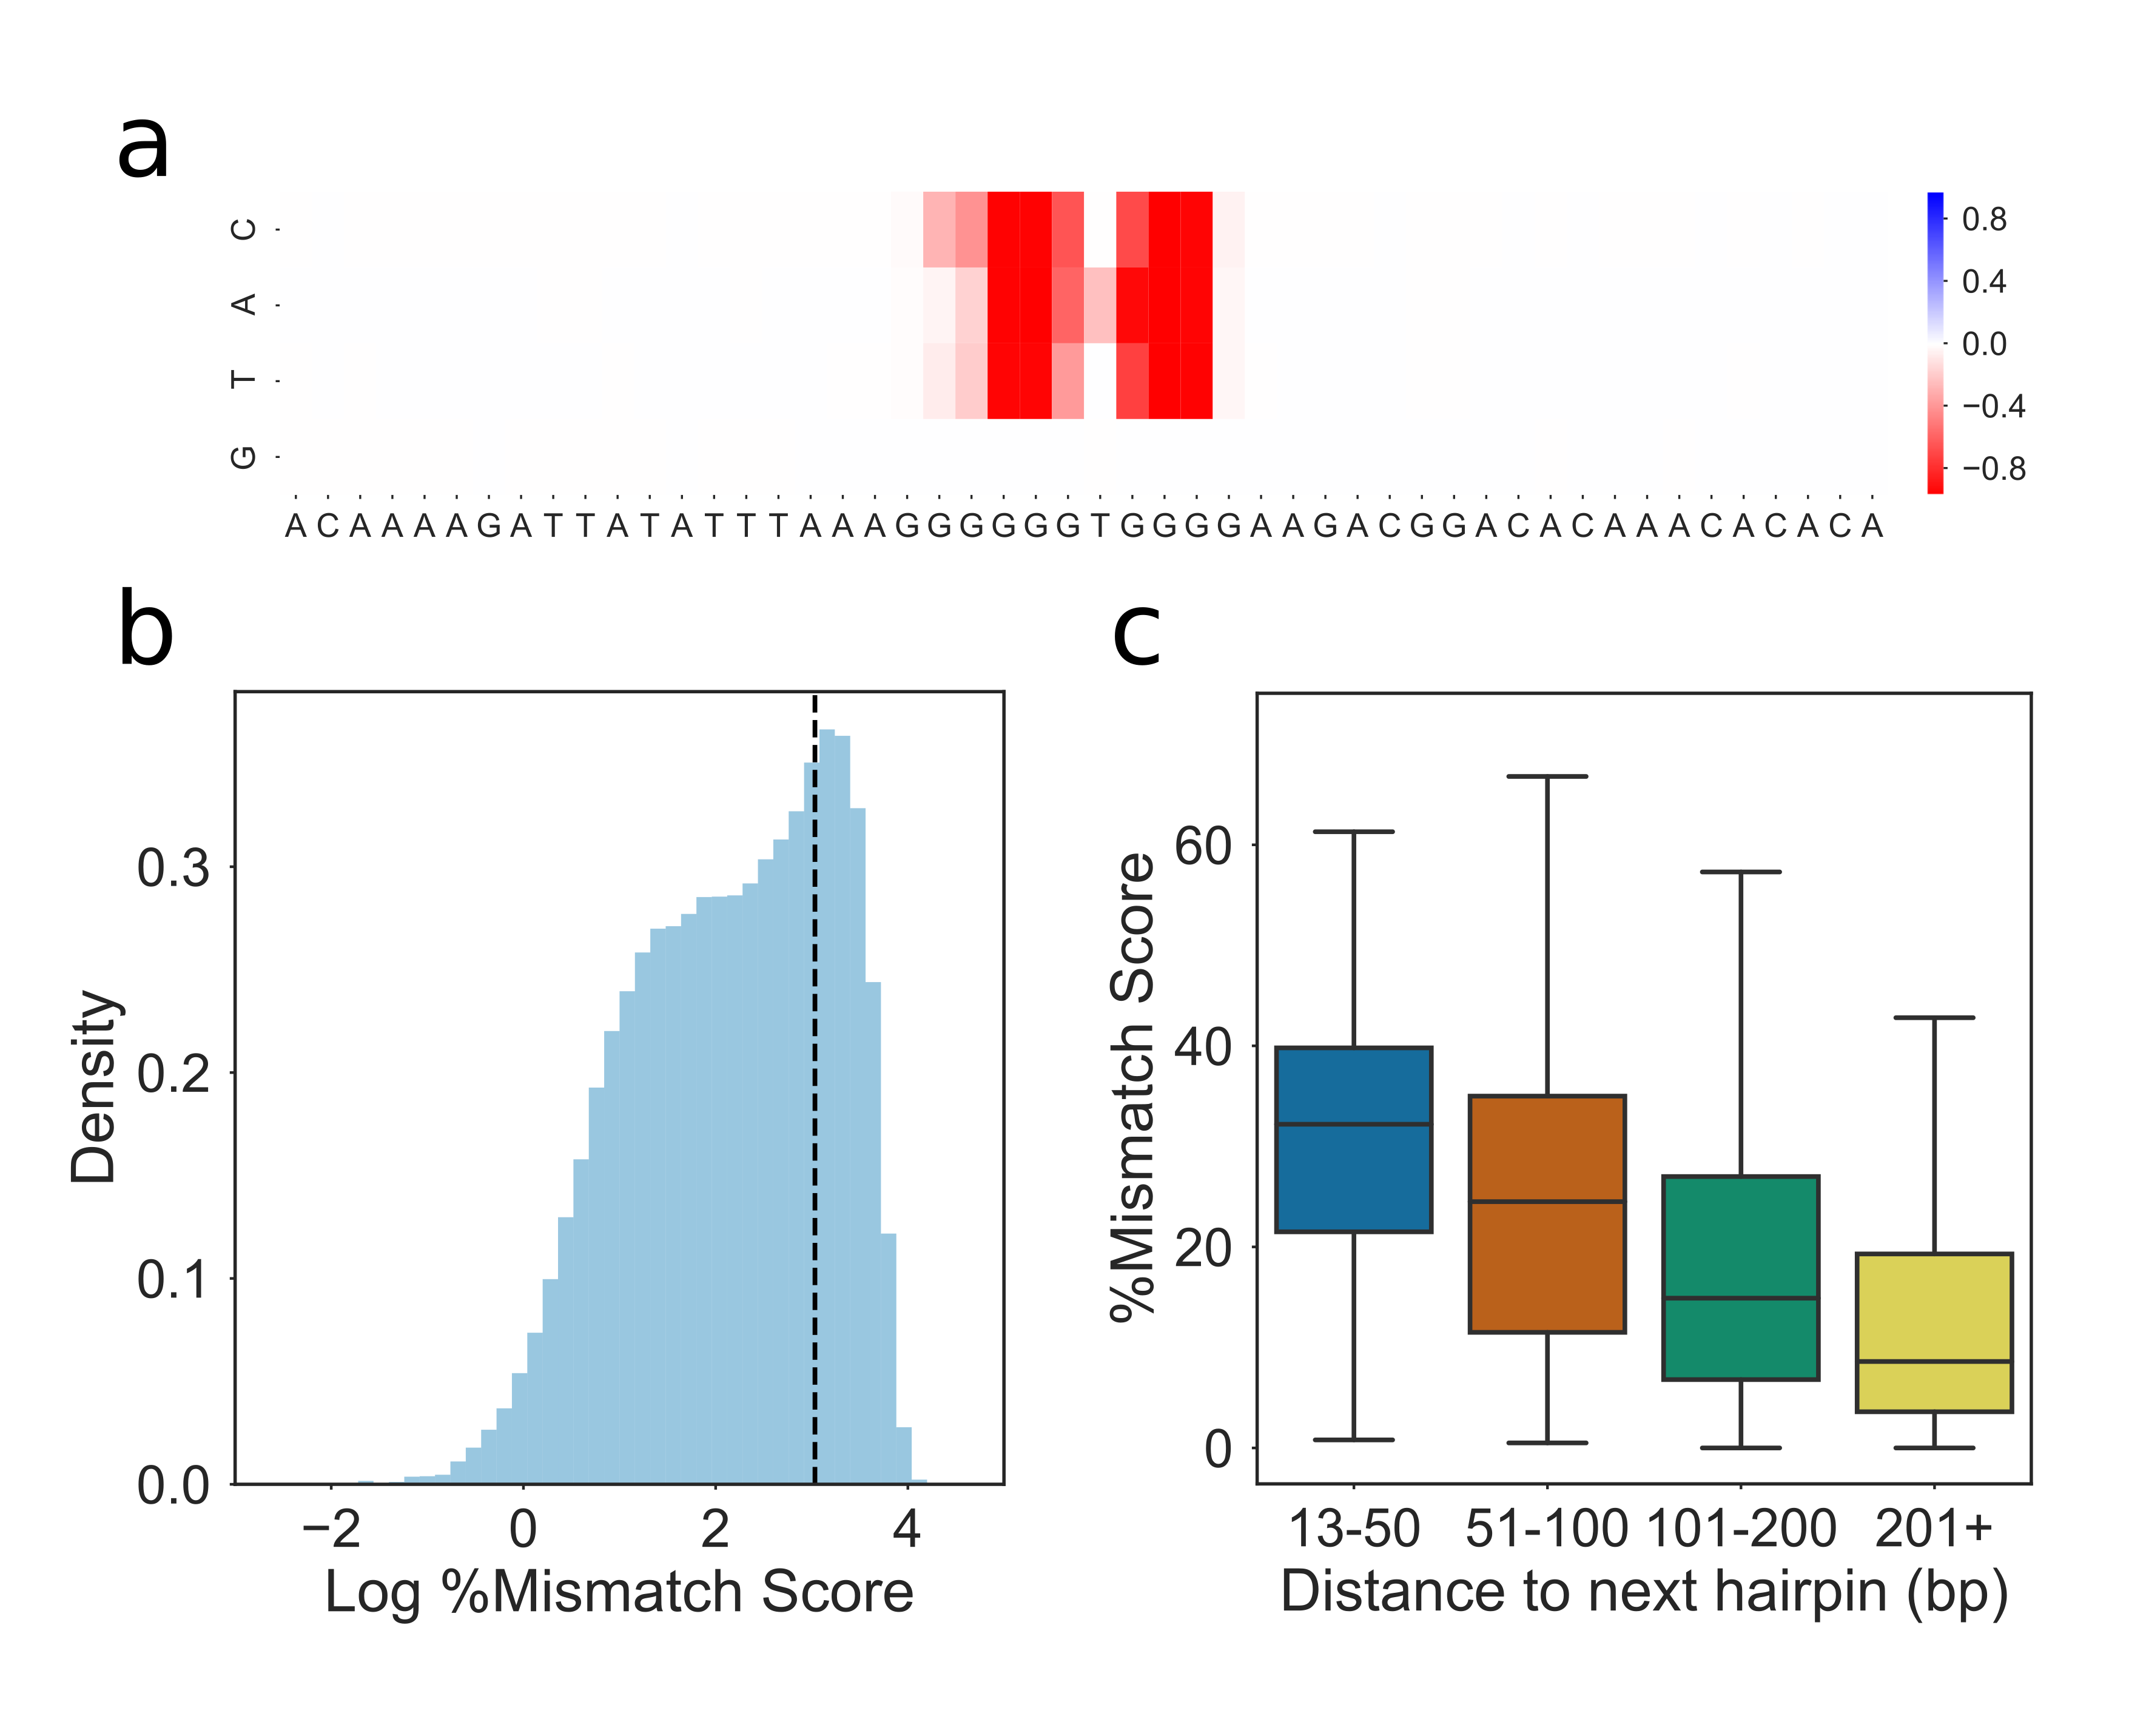
\includegraphics[width=\textwidth,height=562pt,keepaspectratio]{chapter_3/figures/g_hairpin.png}
\caption[Identification of G-hairpin structures by G4Seeqer Mutation Maps]{\textbf{Identification   of   G-hairpin   structures   by   G4Seeqer   Mutation   Maps}   \textbf{a)}   Mutation   map   showing   the   a   high   scoring   (0.99)   G4Seeqer   motif   which   may   form   a   G-hairpin.   Mutation   of   any   base   in   the   core   motif   is   sufficient   to   reduce   the   score   by   up   to   80\%.   \textbf{b)}   Histogram   of   log   percentage   mismatch   score   for   motifs   conforming   to   a   G-hairpin   like   pattern.   The   bimodal   distribution   suggests   that   many   of   these   motifs   form   structures   which   disrupt   polymerase   in   the   presence   of   potassium.   \textbf{c)}   Boxplot   showing   the   relationship   between   \%mm   score   and   distance   to   next   G-hairpin   for   G-hairpin   structures.   The   negative   correlation   suggests   G-hairpins   might   interact   with   other   relatively   distant   hairpins   to   form   G4s.   \label{hairpin}}
\end{figure}

\newpage

\hypertarget{loop-length-and-g4-stability}{%
\subsection{Loop Length and G4
stability}\label{loop-length-and-g4-stability}}

To determine whether G4Seeqer probability scores supported previous work
on the relationship between G4 loop length and stability, we first
downloaded UV melting temperatures for three tetrad G4 sequences from
Table 1 of Guédin et al.~2010. The majority of these G4 sequences
contain only runs of Gs and Ts. In each experiment, one or two of the
three T loops were held at a constant length of either 1 or 3, and the
other loops varied from 1 up to 15 bp in length (Guédin et al., 2010).
For each sequence, we produced 1000 sequences padded to 128bp (the input
length of G4Seeqer) using randomly generated bases, and used G4Seeqer to
predict the stability. We found a very strong correlation (Spearmans rho
0.93, p = 1.1e-35) between empirically determined melting temperature in
potassium, and G4Seeqer score (Fig. \ref{tm}), suggesting that G4Seeqer
is successfully capturing information about G4 structure which is
transferable between conditions. The midpoint of the curve appears to
suggest that a melting temperature of around 65 degrees Celsius is
required for significant mismatches to occur in the G4Seq dataset. We
also noted that G4seeqer output was more variable for sequences with
lower melting temperatures, suggesting that sequence context may be more
important for these G4s.

\newpage

\begin{figure}[htbp]
\centering
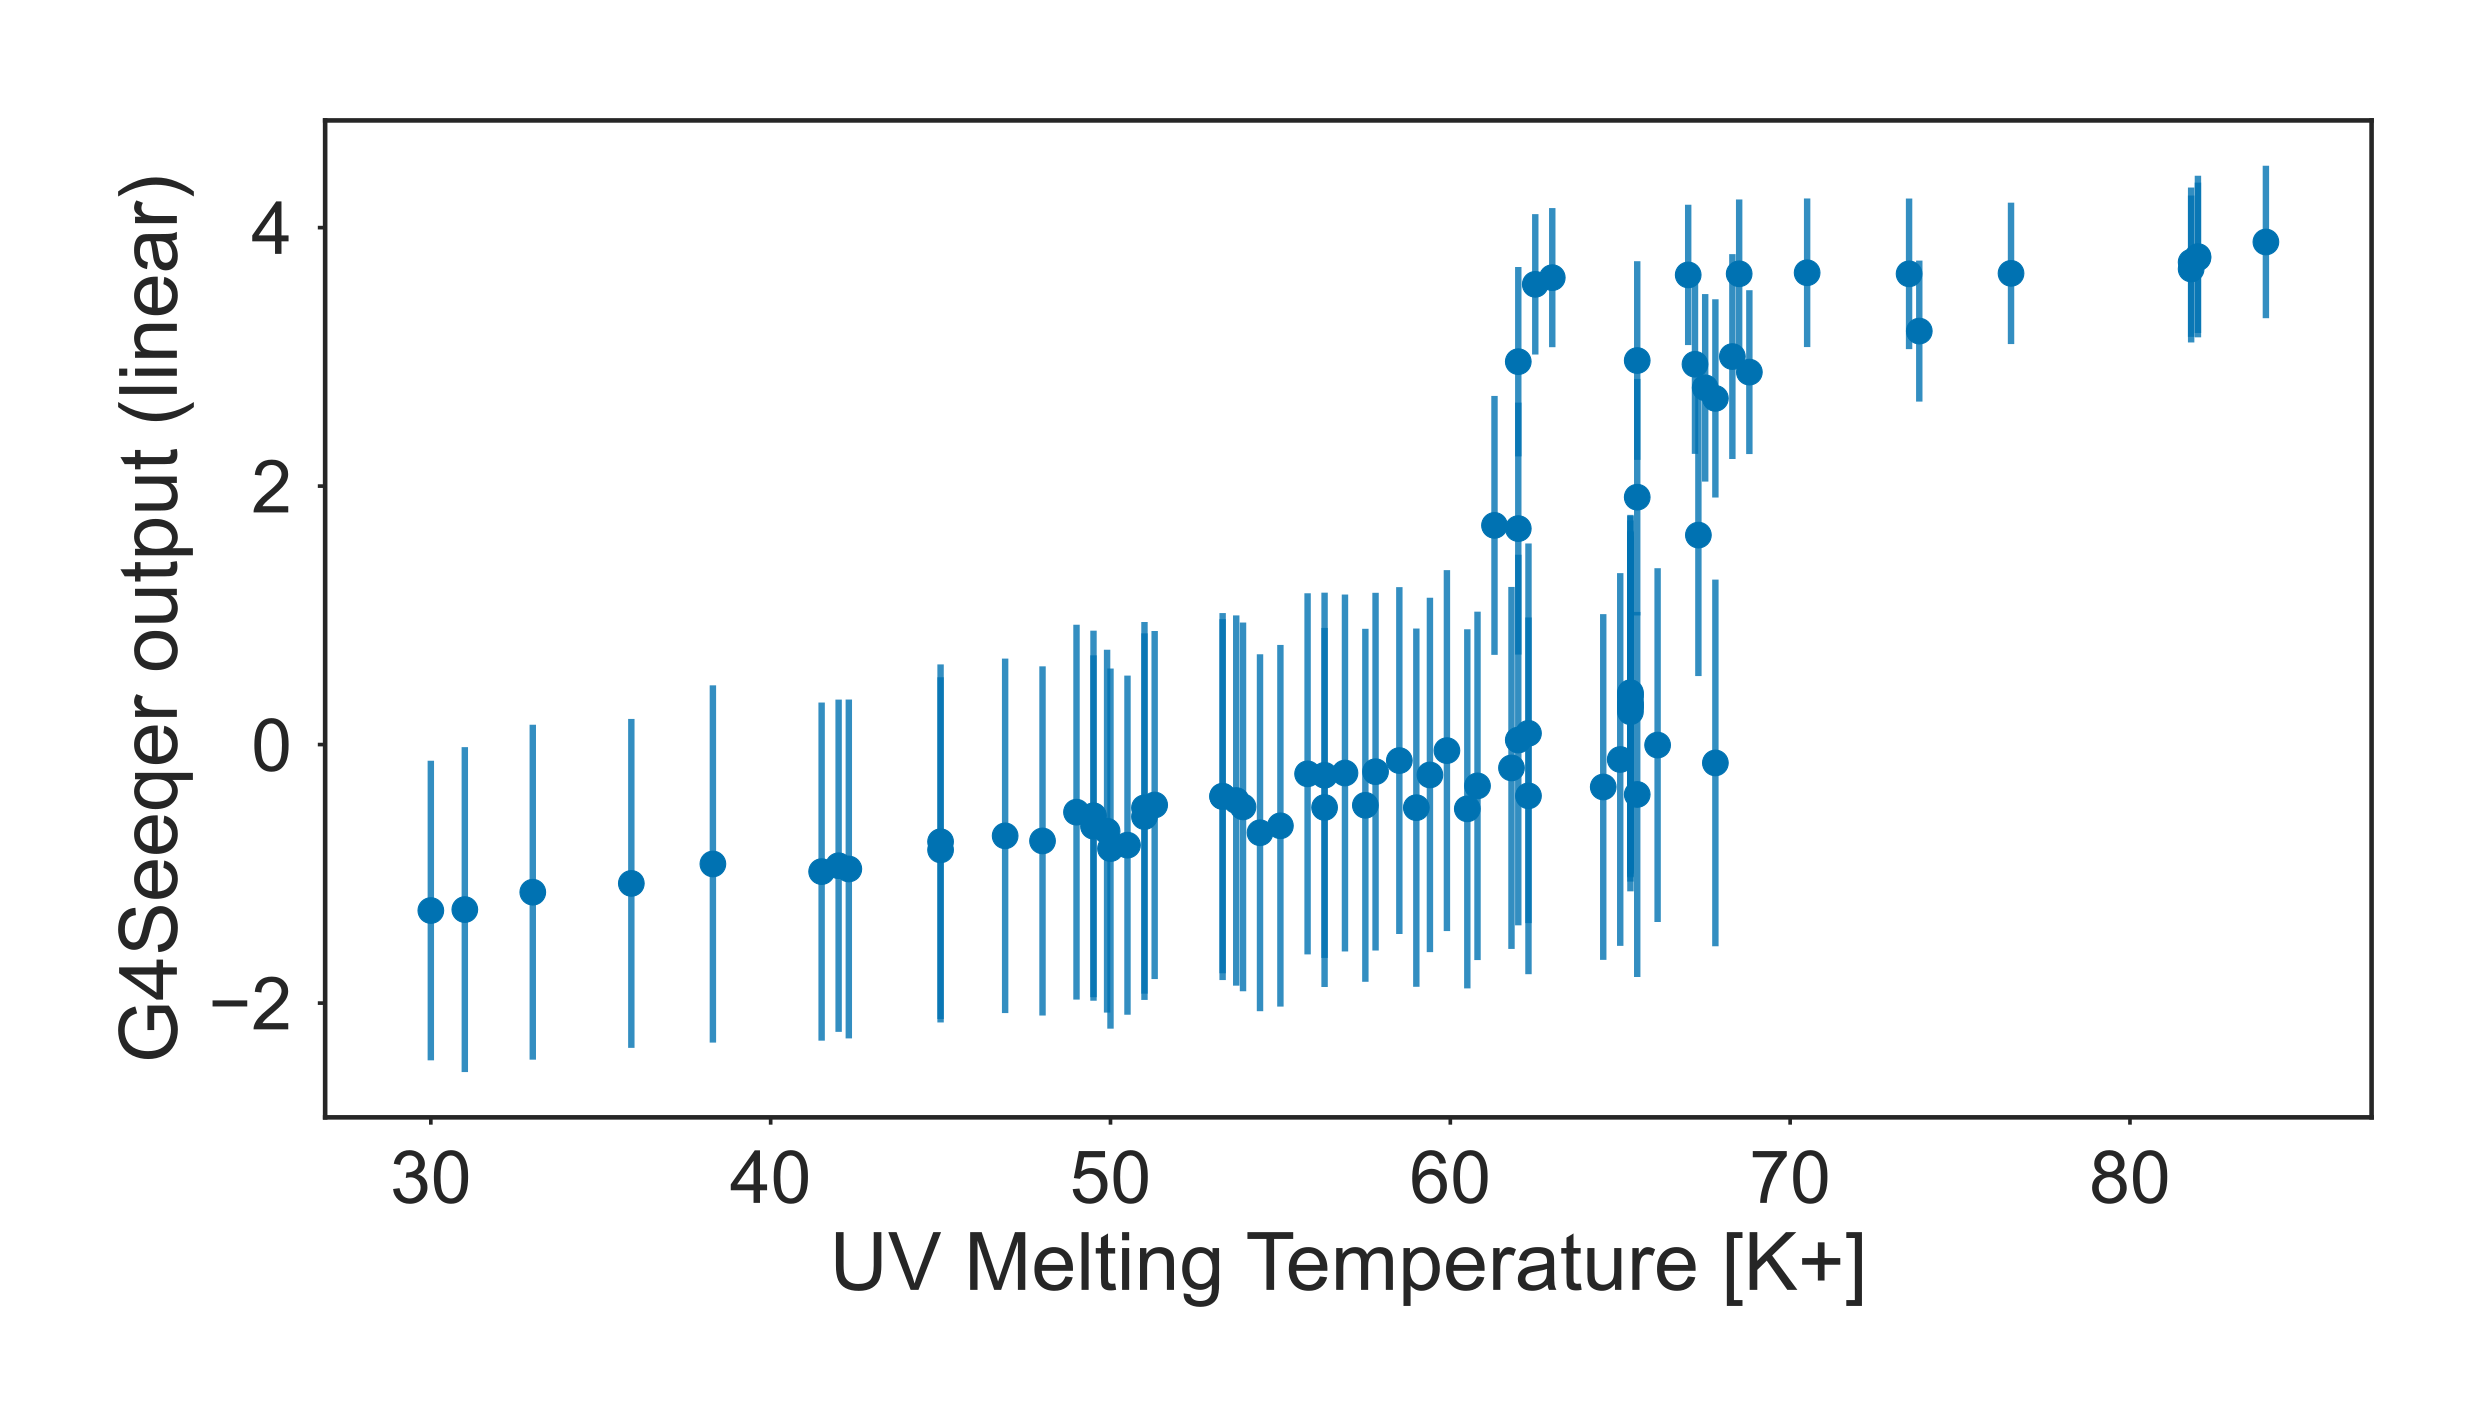
\includegraphics[width=\textwidth,height=562pt,keepaspectratio]{chapter_3/figures/tm_vs_score.png}
\caption[G4Seeqer scores correlate with experimentally determined melting temperatures]{\textbf{G4Seeqer   scores   correlate   with   experimentally   determined   melting   temperatures}   Scatter   plot   showing   median   G4Seeqer   scores   vs. UV   melting   temperature   for   sequences   from   Guédin   et   al. 2010.   Error   bars   are   68\%   confidence   intervals   generated   from   1000   iterations   of   prediction   with   randomly   generated   flanking   sequences.   \label{tm}}
\end{figure}

\newpage

We next performed a similar \emph{in silico} experiment to that of
Guédin et al., whereby we generated random QuadParser conforming G4
sequences with two loop lengths held at 1bp and the third varied from
1-60bp. Loop regions were constructed by randomly selecting from A C or
T. The G4Seeqer score for these sequences was then generated.
Unsurprisingly, we found that G4Seeqer score reduced with increasing
loop length. This effect was strongest for the central loop of the G4,
presumably because varying this loop has a greater effect on the ability
to form stable G-triplex intermediates (Fig. \ref{loop_len}a). We then
set the length of the non-varying loops to 3bp and re-ran the analysis
for third loop length 1-60bp. For these PG4s, we found that the
probability of G4 prediction was much more sensitive to longer loop
lengths (Fig \ref{loop_len}c). There was also no longer a strong
difference in prediction when varying the central loop, compared to
either loops 1 or 3, possibly suggesting that triplex formation in these
sequences is less common.

\newpage

\begin{figure}[htbp]
\centering
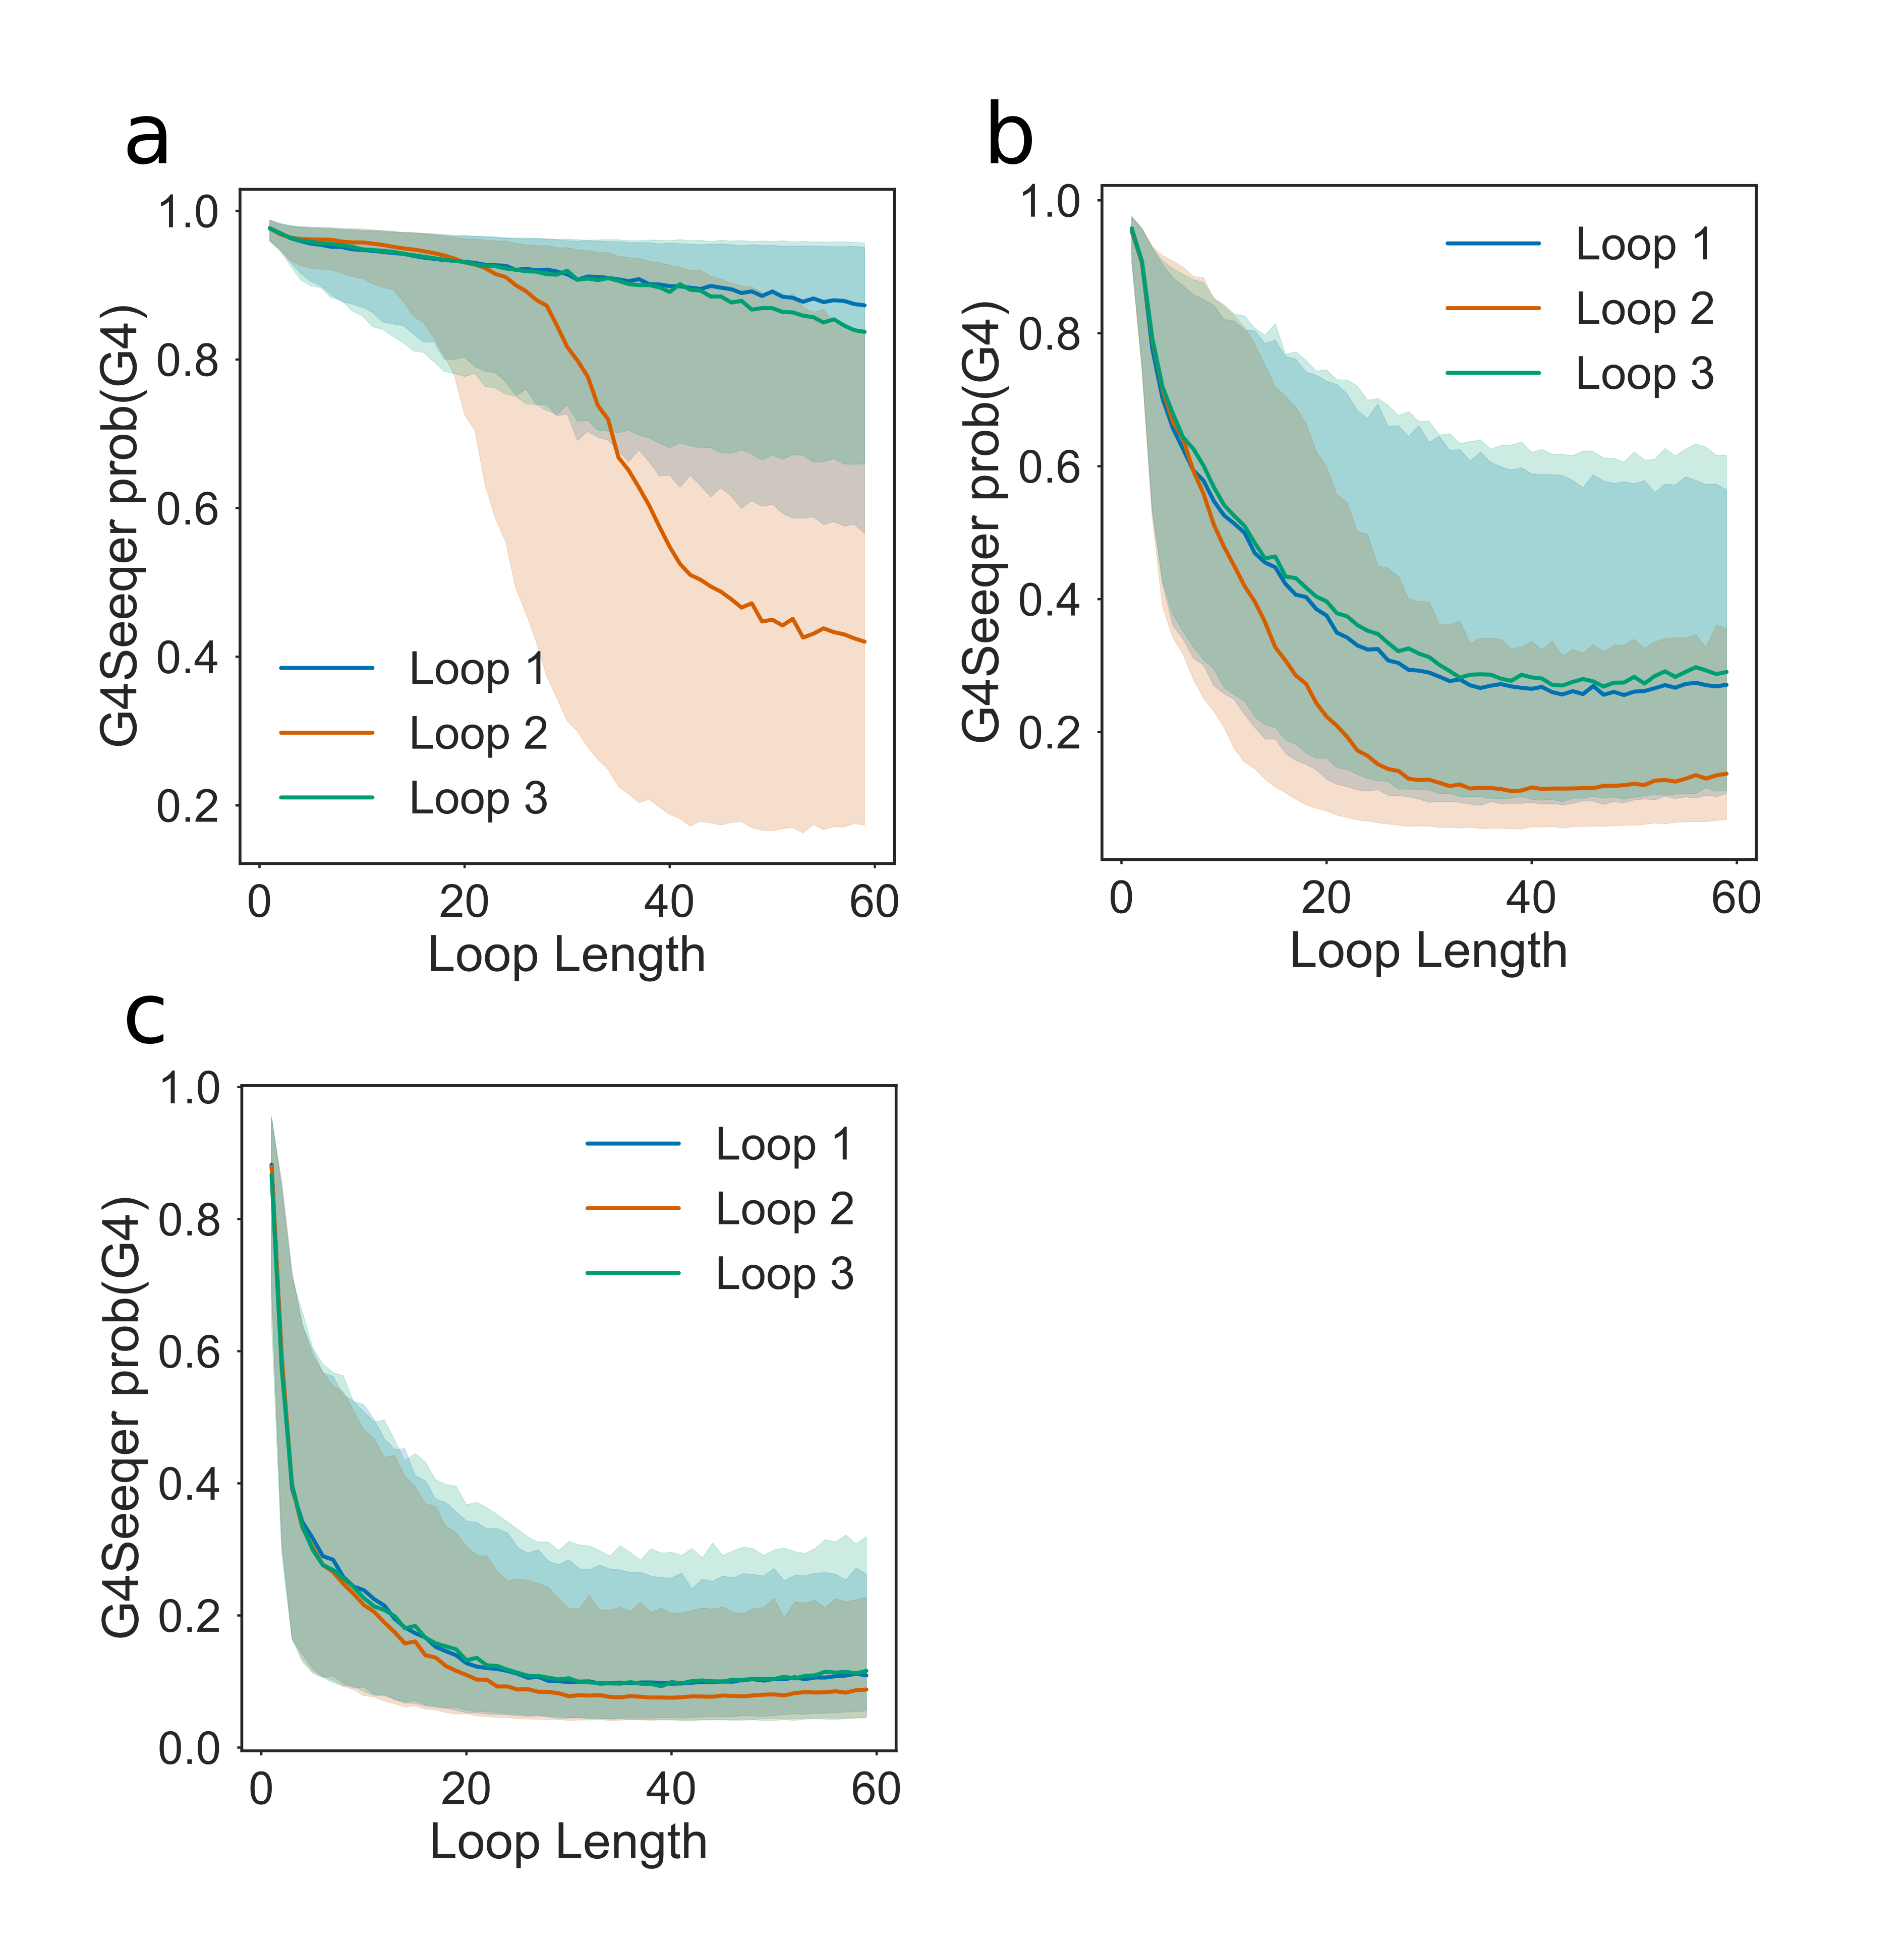
\includegraphics[width=\textwidth,height=562pt,keepaspectratio]{chapter_3/figures/loop_length.png}
\caption[Effect of increasing loop length on G4Seeqer score]{\textbf{Effect   of   increasing   loop   length   on   G4Seeqer   score}   \textbf{a)}   Effect   of   loop   length   on   predicted   G4   stability   when   other   loops   are   held   at   a   constant   length   of   \textbf{a)}   1bp,   \textbf{b)}   2bp   or   \textbf{c)}   3bp.   Median   value   and   68\%   confidence   intervals   are   produced   using   5000   randomly   generated   sequences   (including   flanking   regions   and   loop   contents)   for   each   pattern   analysed.   \label{loop_len}}
\end{figure}

\newpage

\hypertarget{effect-of-g-register-on-g4-stability}{%
\subsection{Effect of G-register on G4
stability}\label{effect-of-g-register-on-g4-stability}}

Work by Harkness and Mittermaier has indicated that extra Guanines in
some G-runs of a G4 forming sequence might increase the G4 forming
potential of the sequence, by allowing exchange between different G4
conformations (Harkness and Mittermaier, 2016). They termed this effect
G-register. We analysed the G4seq dataset and the G4Seeqer model outputs
to determine whether there was evidence of a relationship between
stability and G-register. Firstly, for all PG4s in the human genome
conforming to the three tetrad Quadparser motif, we counted the number
of G-runs which contained four Gs rather than three. These motifs were
then intersected with the G4seq dataset to identify the \%mm score. We
found that G4seq motifs with greater G-register indeed tend to have
higher mismatch scores (Fig. \ref{register}b). To test whether G4seeqer
had successfully identified this pattern, we then randomly generated
three tetrad PG4 sequences with loop lengths of 3bp, and introduced
addition guanines to increase the G-register. Higher G-register strongly
increased the G4Seeqer score of the sequence, showing that the model has
successfully learned this feature of G4s (Fig. \ref{register}a).

\newpage

\begin{figure}[htbp]
\centering
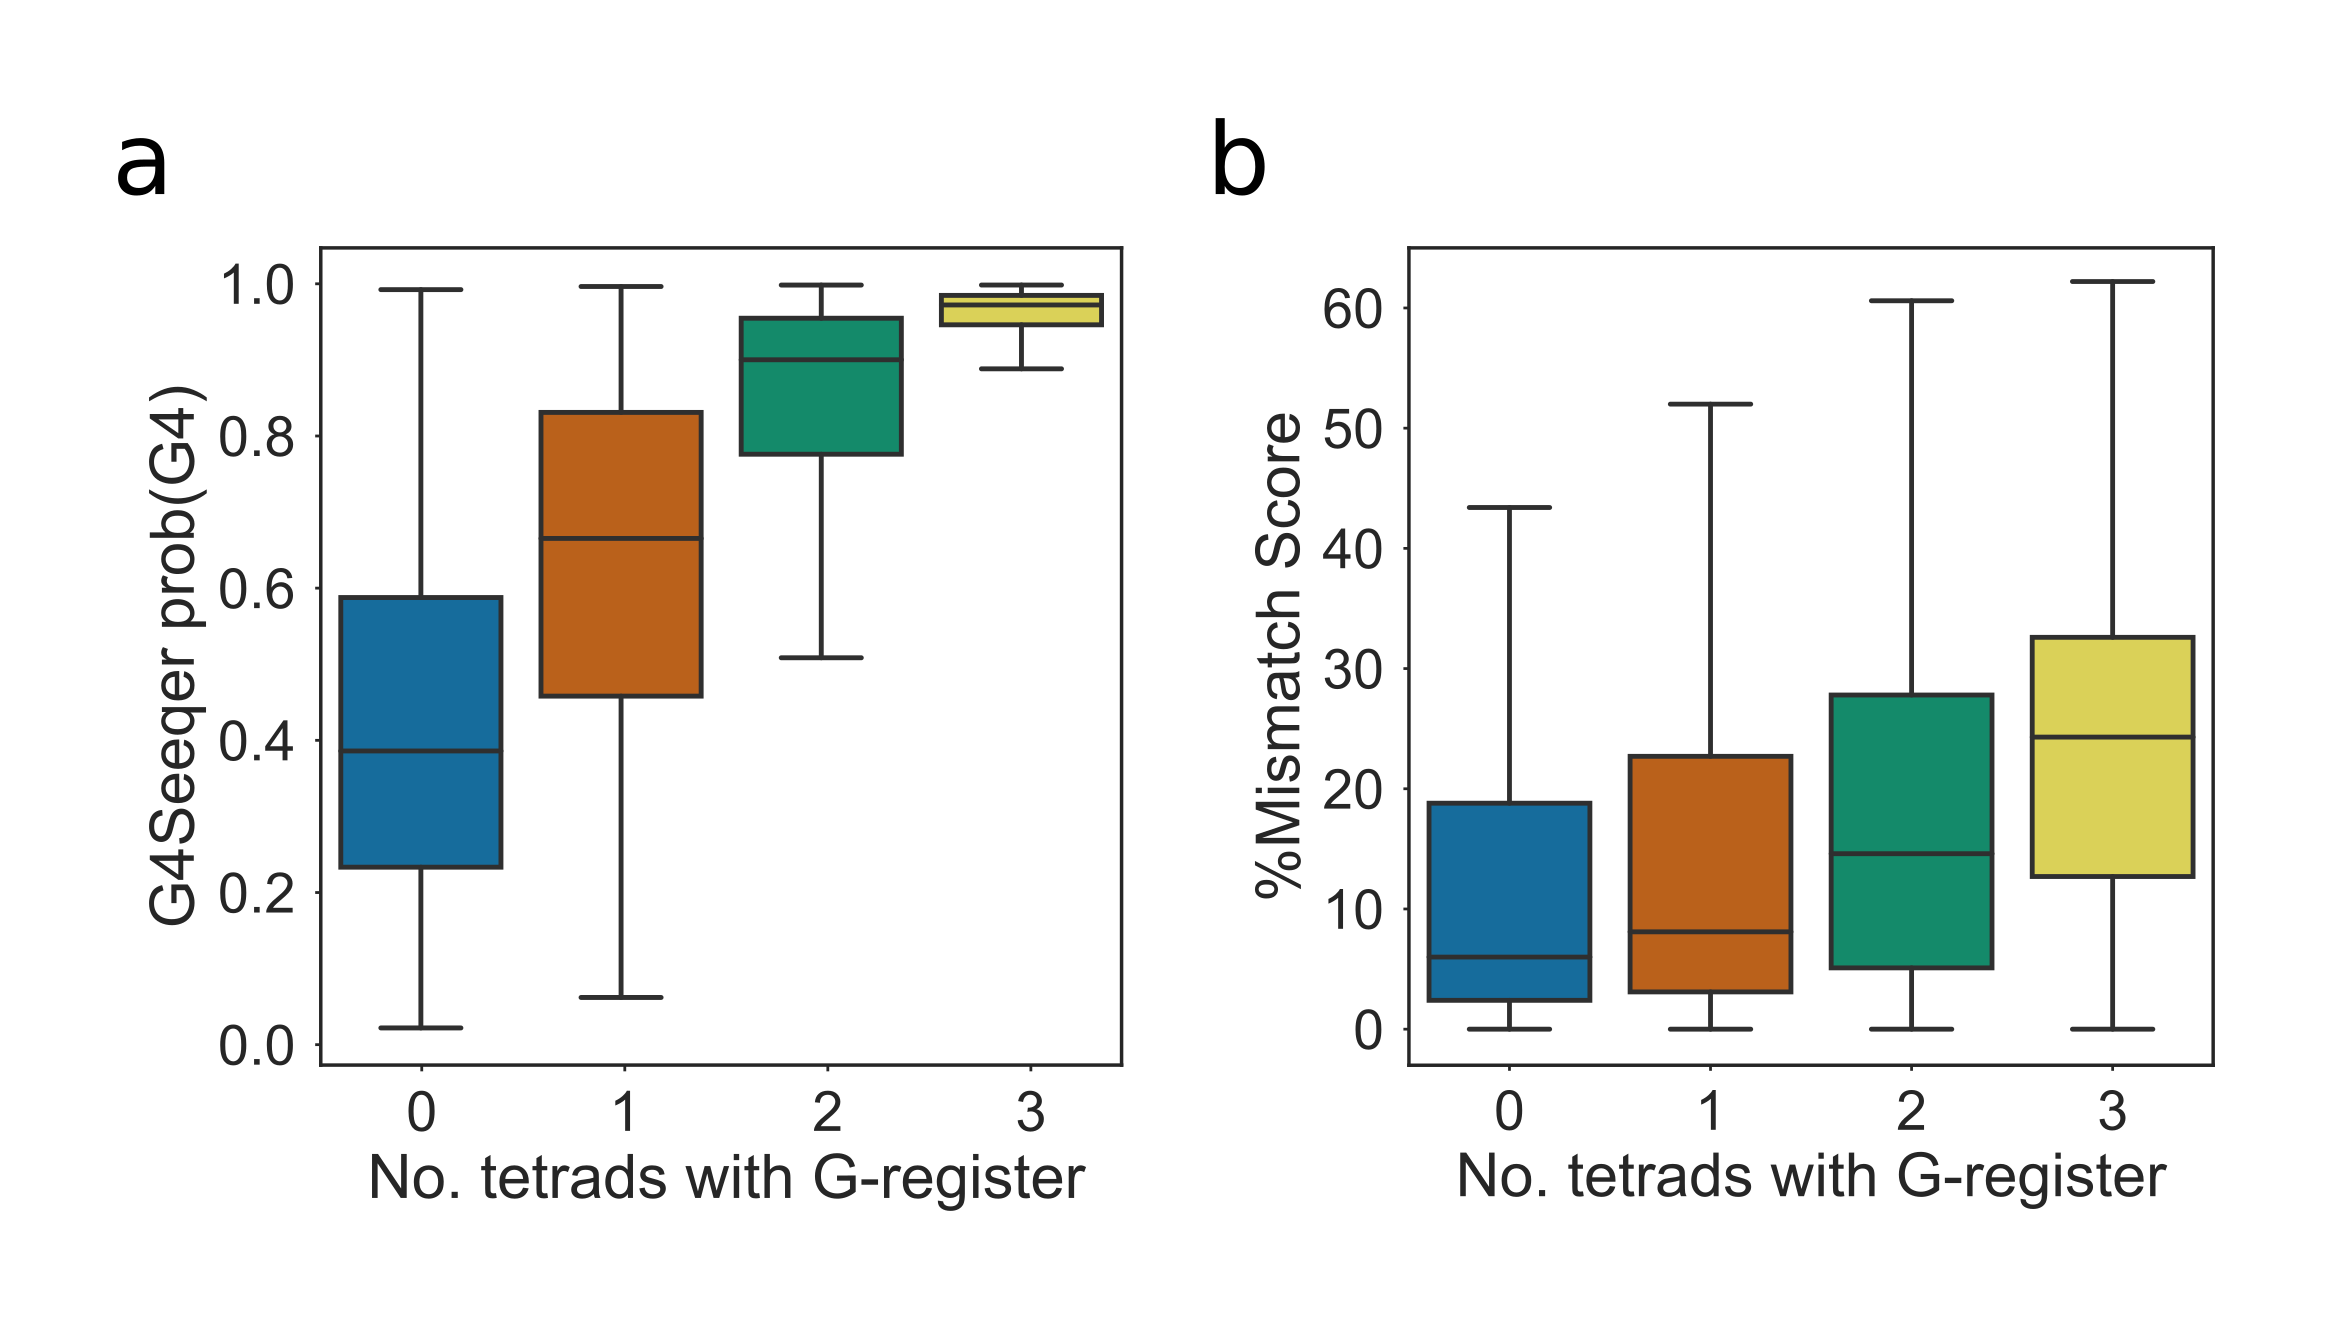
\includegraphics[width=\textwidth,height=562pt,keepaspectratio]{chapter_3/figures/g_register.png}
\caption[Scoring of G-register effects by G4Seeqer]{\textbf{Scoring   of   G-register   effects   by   G4Seeqer}   \textbf{a)}   Boxplot   showing   G4Seeqer   scores   for   randomly   generated   3   tetrad   Quadparser   conforming   sequences   with   zero   to   three   additional   Guanines   per   run,   referred   to   by   Harkness   and   Mittermaier   as   G-register.   \textbf{b)}   Boxplot   showing   relationship   between   G-register   and   \%mm   score   in   the   G4Seq   dataset   for   Quadparser   conforming   G4s.   \label{register}}
\end{figure}

\newpage

\hypertarget{applicability-of-the-model-to-other-genomes}{%
\subsection{Applicability of the model to other
genomes}\label{applicability-of-the-model-to-other-genomes}}

Whilst the Human genome contains a large number of G4 forming sequences,
this is not even close to saturating the population of all potential
G4s. Indeed, simply considering the Quadparser motif with loop lengths
up to 12, there are \(1.1\times10^{22}\) different conforming sequences,
many orders of magnitude more than there are bases in the human genome.
It is probable that the human genome contains a biased subpopulation of
all G4s. This might mean that the G4Seeqer model does not generalise
well to other genomes which contain different subpopulations. As an
example, we analysed 3 tetrad Quadparser motifs from hg19, where all
three loops were of length 3. There are \(4^9\) (262,144) possible
sequences fitting this description, of which only 1.4\% (3,748) appear
in hg19 (Fig. \ref{g4_space}a). The motifs that did appear tended to be
those with lower complexity, as measured by the number of distinct
dinucleotides in the sequence, than the total possible population (Fig.
\ref{g4_space}b). The PG4 space of the \emph{M. musculus} genome was
also measured, and found to contain 1.7\% (4330) of all possible 3
tetrad PG4s with loop length 3. There was a strong overlap of 27\% (p
\textless{} 2.2e-308) between sequences in the human and mouse genomes,
however, suggesting that at least for this pattern, the PG4 populations
of these genomes are comparable. The more complex the PG4 motifs become,
however, the more likely it is that these subpopulations will be very
different. There are clear differences in dinucleotide content between
different genomes, which are often a result of differences in amino acid
composition of proteins, or other environmental factors such as
temperature. For genomes whose last common ancestor with \emph{Homo
sapiens} was longer ago, this divergence may be much greater. These
systemic differences between may result in patterns to which the model
has not previously been exposed, and reduce the performance of the
model. G4Seeqer, or any other models which are trained on sequences from
a single genome, should therefore be used with caution on others.

\newpage

\begin{figure}[htbp]
\centering
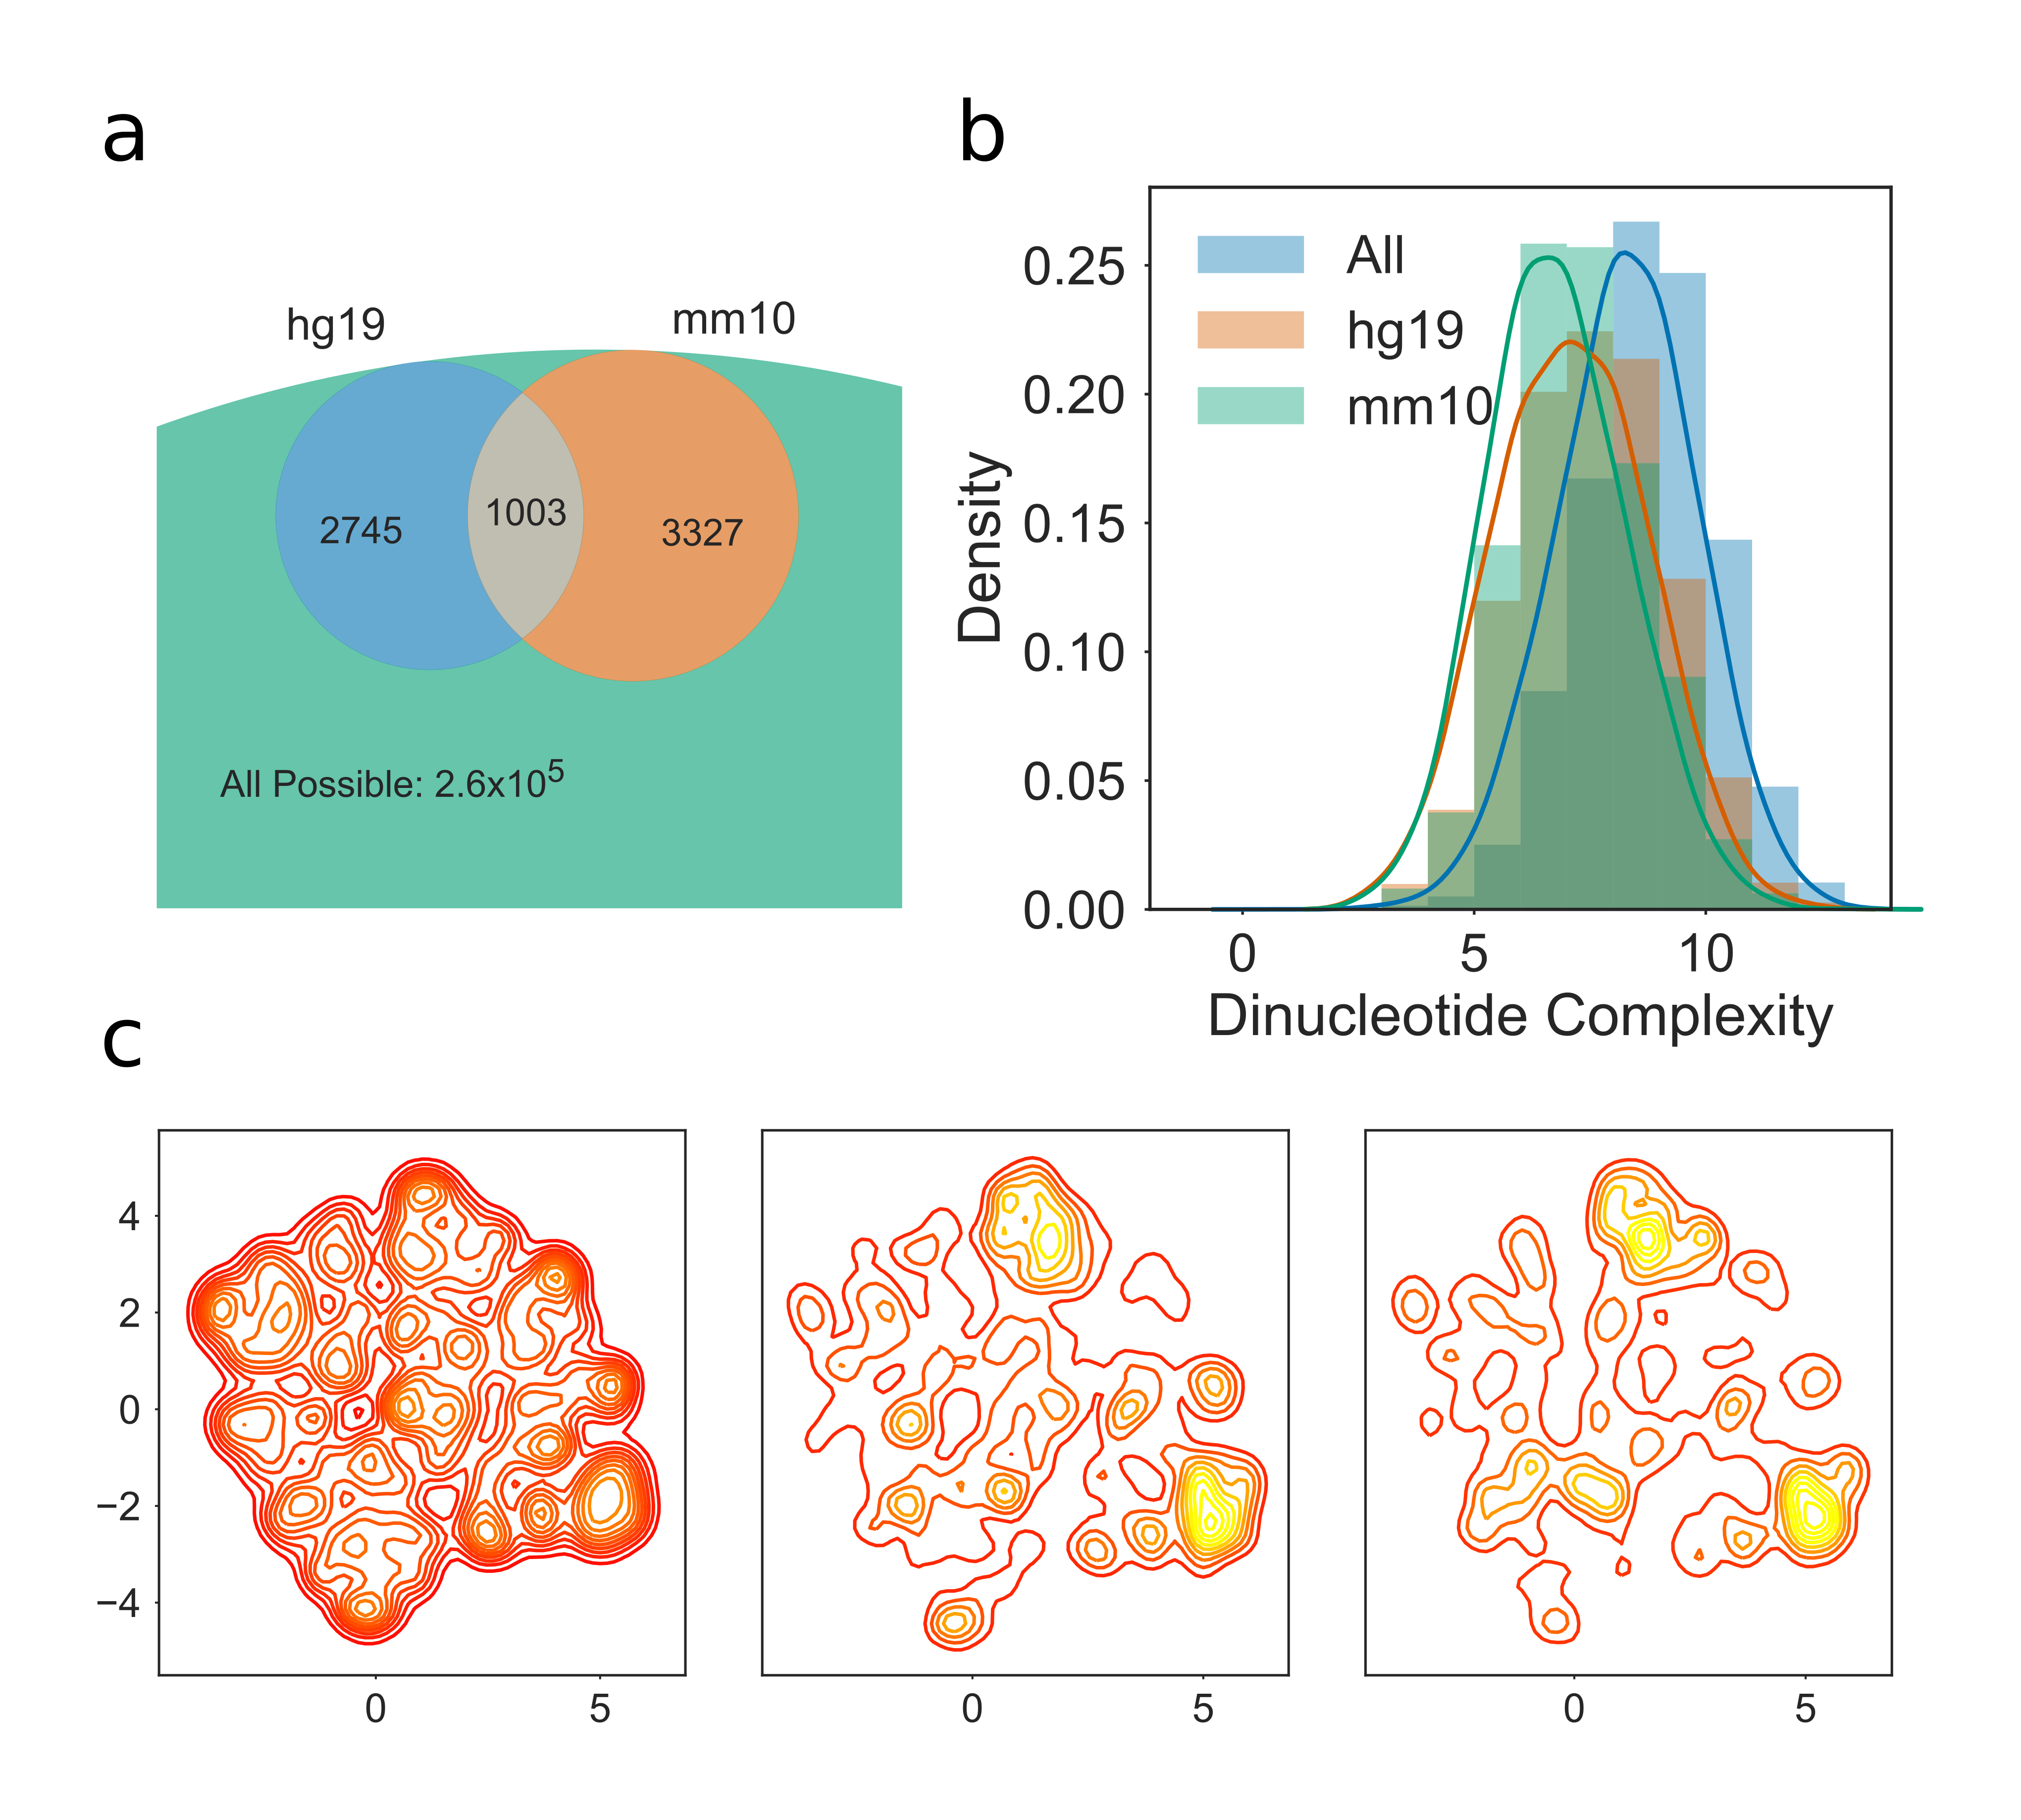
\includegraphics[width=\textwidth,height=562pt,keepaspectratio]{chapter_3/figures/g4_space.png}
\caption[Human and mouse genomes contain different G4 subpopulations]{\textbf{Human   and   mouse   genomes   contain   different   G4   subpopulations}   \textbf{a)}   Venn   diagram   showing   overlap   of   3   tetrad   Quadparser   motifs   populations   with   loop   lengths   of   3bp   in   the   human   (hg19)   and   mouse   (mm10)   genomes,   compared   to   all   possible   sequences.   \textbf{b)}   Histogram   and   kernel   density   estimate   of   dinucleotide   complexity   for   human,   mouse   and   all   possible   3   tetrad   Quadparser   motifs   with   loop   length   of   3bp.   \textbf{c)}   2D   Kernel   density   estimate   plot   showing   distribution   of   all   possible   tetrad   Quadparser   motifs   (left),   those   found   in   the   human   genome   (centre)   and   those   found   in   the   mouse   genome.   Dimensionality   reduction   was   conducted   using   UMAP   with   Hamming   distance   as   the   metric.   \label{g4_space}}
\end{figure}

\newpage

\hypertarget{conclusion}{%
\subsection{Conclusion}\label{conclusion}}

We present G4Seeqer, the first Convolutional/Recurrent Neural Network
model for prediction of G Quadruplex forming structures. G4Seeqer is
implemented in Python, using Cython for speed-up of G4Hunter candidate
region proposal, and \texttt{Keras} with \texttt{Tensorflow} backend for
neural network prediction (Abadi et al., 2016; Chollet, 2018). Weights
have been trained on the G4Seq dataset (Chambers et al., 2015) and
transfer learned to the rG4Seq dataset (Kwok et al., 2016), to produce
models tailored for DNA and RNA G4s, respectively. It is able to make
predictions on the whole human genome in approximately 1 hour on a 8
core i7 desktop computer with 16GB RAM. Because G4Seeqer is trained
directly upon sequences from the human genome, rather than on derived
sequence features, it is able to identify patterns in the G4Seq dataset
that have not previously been reported, as well as removing false
positive sequences which are flagged by pattern matching techniques.
This greatly improves the accuracy of the model on various \emph{in
vitro} and \emph{in vivo} datasets, from stabilities determined by UV
melting to genomic regions identified by BG4 ChIP-seq (Hänsel-Hertsch et
al., 2016).

\newpage

\hypertarget{global-analysis-of-predicted-g-quadruplexes-in-the-arabidopsis-thaliana-genome}{%
\chapter{\texorpdfstring{Global analysis of Predicted G-Quadruplexes in
the \emph{Arabidopsis thaliana}
genome}{Global analysis of Predicted G-Quadruplexes in the Arabidopsis thaliana genome}}\label{global-analysis-of-predicted-g-quadruplexes-in-the-arabidopsis-thaliana-genome}}

\label{chap:g4_distribution}

\hypertarget{introduction-2}{%
\section{Introduction}\label{introduction-2}}

\emph{Arabidopsis thaliana} is a member of the \emph{Brassicaceae}
family, which contains many important crop species. Whilst it is not of
major agricultural importance itself, its short generation time and
amenability to transformation has made it an extremely important model
for genetic and genomic studies of plants. The genome of Arabidopsis is
small, with various estimates putting its size between 125-150Mb (The
Arabidopsis Genome Initiative, 2000; Bennett et al., 2003). This is
approximately 80Mb less than the closely related species
\emph{Arabidopsis lyrata}, suggesting a recent genome contraction event
(Hu et al., 2011). Hu et al.~identified that the majority of this genome
contraction is the result of deletion of transposable element sequences,
and shortening of intergenic and intronic sequences. Despite the extreme
reduction in size, \emph{A. thaliana} has only 17\% fewer genes than
\emph{A. lyrata} (Hu et al., 2011). This evidence points to selection
for a compact genome.

Many genomes, including most mammalian genomes, exhibit periodic GC
content changes on the level of tens to hundreds of kilobases. This is
referred to as the isochore structure (Eyre-Walker and Hurst, 2001).
GC-rich isochores exhibit higher gene density (Mouchiroud et al., 1991),
and greater G4 forming potential (Maizels, 2012). In contrast, the
genomes of angiosperms, including Arabidopsis, do no have a clear
arrangement of GC rich regions into isochores, and the GC content of the
third codon position of gene CDSs is weakly correlated with the GC
content of the flanking intergenic sequence (Tatarinova et al., 2010).
GC content tends to be greater in exons than in intergenic or intronic
sequence (Zhu et al., 2009). Furthermore, several authors have noted a
negative gradient of GC richness across exons and introns, with GC
content greatest at the TSS (Wong et al., 2002; Glémin et al., 2014).
This suggests there may be greater G4 forming potential at the TSS
proximal end of plant genes.

Previous analyses of PG4 densities in plant genomes have been conducted
by Mullen et al.~2010, and Garg et al.~2016. Mullen et al.~identified
only 1200 three tetrad PG4s in the Arabidopsis genome (Mullen et al.,
2010; Garg et al., 2016). Using a Markov chain modelled genome with a
window size of 100bp, Mullen et al.~demonstrated that this represents a
greater than two fold depletion of three tetrad PG4 sequences (Mullen et
al., 2010). This is a much greater depletion than in the human genome,
which Huppert \& Balasubramanian suggested has 1.4 times fewer three
tetrad PG4s than should be expected by chance (Huppert and
Balasubramanian, 2005). 70\% of three tetrad PG4s were found in
intergenic regions, and of these, 20\% corresponded to the Arabidopsis
telomeric sequence. Despite genic regions having a higher GC content
(38.9\%) than intergenic regions (31.1\%), Mullen et al.~found that the
PG4 density of intergenic regions was still higher (genic 4.6 PG4s/Mb,
intergenic 16.7 PG4s/Mb). These are not average windowed densities,
however, and so intergenic densities may be skewed by the extremely PG4
dense telomeric and centromeric regions. Mullen et al.~also predicted
43000 two tetrad PG4s in the Arabidopsis genome, using a loop length of
up to 4bp. This did not constitute an enrichment or depletion over the
expected levels from the Markov chain modelled genome. They noted that
80\% of two tetrad PG4s occur inside genic regions, however, and
suggested that this might lead to their formation in mRNA (Mullen et
al., 2010, 2012).

In this chapter, we briefly examine the PG4 density of Arabidopsis
compared to other plant genomes, and use metagene profiles to examine
the distribution of PG4s across gene models. Finally, we develop a new
simulation method to test whether PG4 motifs in CDS regions are
hardcoded by protein coding sequences.

\newpage

\hypertarget{materials-and-methods-1}{%
\section{Materials and Methods}\label{materials-and-methods-1}}

\hypertarget{plant-genome-pg4-analyses}{%
\subsection{Plant genome PG4 analyses}\label{plant-genome-pg4-analyses}}

The genomes of 48 multicellular land plants were downloaded over FTP
from Ensembl Plants Release 39. This included 22 Monocotyledons, 23
Dicotyledons, and 3 Non-flowering plants. The genomes of four metazoans,
\emph{Drosophila melanogaster} (fruit fly), \emph{Danio rerio}
(zebrafish), \emph{Mus musculus} (mouse) and \emph{Homo sapiens}
(human), were downloaded from Ensembl release 92. Bed files of
non-overlapping PG4 predictions were generated using \texttt{g4predict},
an in house Quadparser matching program. PG4 densities were measured for
either two tetrad PG4s, or three or more tetrad PG4s, and a maximum loop
length of 7bp was used. Average PG4/Mb densities were generated by using
\texttt{bedtools\ makewindows} to create non-overlapping windows of 1Mb
in size, and then using \texttt{bedtools\ intersect} in count mode to
count the number of PG4s per Mb (Quinlan and Hall, 2010). The mean
density for each genome was then calculated using \texttt{awk} (Aho et
al., 1988). Genome size for each species was calculated from the total
size of the fasta file. Genomes were annotated as Monocots or Dicots
using metadata downloaded from the UniProt taxonomy database. Scatter
plots were generated using \texttt{matplotlib} and \texttt{seaborn}
(Hunter, 2007; Waskom et al., 2014).

\hypertarget{metagene-profiles}{%
\subsection{Metagene Profiles}\label{metagene-profiles}}

Shuffled genomes were generated in Python using \texttt{ushuffle} to
shuffle sequences in 20bp windows, maintaining their nucleotide and
dinucleotide contents (Jiang et al., 2008). G content on both strands
was calculated in 20bp windows, using \texttt{bedtools\ makewindows},
\texttt{bedtools\ nuc} and \texttt{awk} (Aho et al., 1988; Quinlan and
Hall, 2010). GC Bed files of non-overlapping PG4s were converted into
BigWig format using \texttt{bedtools\ genomecov} and
\texttt{ucsc-bedGraphToBigWig} (Kent et al., 2010). Gene annotations
were taken from Araport11. Overlapping transcripts of the same gene were
flattened into a single bed12 interval per gene, with the leftmost TSS
and start codon and the rightmost TTS and stop codon (or vice versa for
genes on the negative strand). GC/PG4 coverage arrays for the 500bp
upstream region, 5'UTR, CDS, 3'UTR and 500bp downstream region were then
extracted for each gene using \texttt{pyBigWig} and reinterpolated to
sizes of 50, 20, 100, 20, and 50 respectively (Ryan et al., 2018). These
were then averaged across all genes to produce metaprofiles. Plots were
generated using \texttt{matplotlib} and \texttt{seaborn} (Hunter, 2007;
Waskom et al., 2014).

\hypertarget{reverse-translation-method}{%
\subsection{Reverse Translation
Method}\label{reverse-translation-method}}

Relative frequency of codon usage for all Arabidopsis CDS sequences was
calculated in python. Reverse translation was conducted by translating
CDSs into protein, then randomly selecting codons to represent the
protein, weighting each codon by its usage. 100 reverse translated
potential coding sequences (PCSs) were generated per CDS. G content on
each strand was calculated using 20bp windows and reinterpolated to 100
bins, for both real CDSs and PCSs. PG4 content was calculated using
G4Seeqer and the overlapping Quadparser method. Overlapping PG4s were
flattened into a single interval. PG4s were binned into 100 equally
sized bins per gene, based on the midpoint of the PG4. Resultant
profiles were stored in HDF5 format using \texttt{h5py} (Andrew
Collette, 2013). Averaged profiles across all iterations of reverse
translation, and all genes were generated and plotted using
\texttt{matplotlib} (Hunter, 2007).

\hypertarget{hardcoded-pg4-analysis}{%
\subsection{Hardcoded PG4 Analysis}\label{hardcoded-pg4-analysis}}

For hardcoded PG4 analysis, all overlapping two tetrad PG4 registers in
CDSs were predicted using network analysis with \texttt{networkx}
(Hagberg, Aric; Schult, Daniel; Swart, 2008). G-runs were extracted from
these PG4s, and the position, frame, and resultant protein sequence
coded for by each G-run was calculated. Hardcoded G-runs were identified
by analysing whether it would be possible to use synonymous codons which
do not change the protein sequence, which would abolish the G-run. PG4s
which had G-runs which all code for the same protein motif were labelled
as repetitive. For G-run frequency plots, G-runs which contribute to
multiple PG4s were deduplicated to give only one G-run per position.
G-runs which contributed to both repetitive and non-repetitive PG4
registers were labelled as non-repetitive. For hardcoded PG4 metagene
profiles, PG4s were binned into 100 equally sized bins per CDS, based on
the midpoint of the PG4. All overlapping PG4s were counted in the
profile. The total number of PG4s per bin was counted, and cumulative
frequency metagene profiles were plotted using \texttt{matplotlib}
(Hunter, 2007). Frequency plots of hardcoded PG4s/G-runs,
repetitiveness, and protein motifs were produced using \texttt{seaborn}
(Waskom et al., 2014).

\newpage

\hypertarget{results}{%
\section{Results}\label{results}}

\hypertarget{the-genome-of-arabidopsis-thaliana-poor-in-three-tetrad-pg4s-but-not-two-tetrad-pg4s}{%
\subsection{\texorpdfstring{The genome of \emph{Arabidopsis thaliana}
poor in three tetrad PG4s, but not two tetrad
PG4s}{The genome of Arabidopsis thaliana poor in three tetrad PG4s, but not two tetrad PG4s}}\label{the-genome-of-arabidopsis-thaliana-poor-in-three-tetrad-pg4s-but-not-two-tetrad-pg4s}}

To compare the PG4 density of the Arabidopsis genome to other organisms,
we downloaded the set of 48 land plant genomes available in Ensembl
Plants Release 39, which included 22 Monocotyledons, 23 Dicotyledons,
and 3 Non-flowering plants. The genomes of the metazoans
\emph{Drosophila melanogaster} (fruit fly), \emph{Danio rerio}
(zebrafish), \emph{Mus musculus} (mouse) and \emph{Homo sapiens} (human)
were also analysed. PG4s with three or more were identified using the
Quadparser method and the average density per Megabase was calculated
for each genome. Arabidopsis has the smallest genome of any of the
sequenced plants, estimated at 135Mb (119Mb in the golden path
sequence). It also has one of the lowest three tetrad PG4 densities.
Only 1284 non-overlapping PG4s with three or more tetrads are predicted
to form in the whole Arabidopsis genome, with an average density of 10.4
PG4s/Mb. In comparison, the human genome is extremely PG4 dense, with an
average of 123 PG4s/Mb. Monocot plants also tend to have much greater
PG4 densities than Dicots (median density 59 PG4s/Mb vs.~3.3 PG4s/Mb).
This is likely to result from a greater GC content in Monocot genomes.
Non-flowering plants such as the bryophyte \emph{Physcomitrella patens}
had PG4 densities which resembled those of the Dicots more closely. We
did not find a correlation between PG4 density and genome size
(Spearmans rho = -0.02).

We noted that the PG4 densities of the warm blooded mammals \emph{M.
musculus} and \emph{H. sapiens} are much greater than those of \emph{D.
melanogaster} or \emph{D. rerio}, or any of the plants. The PG4 density
of \emph{Mus musculus} is 227 PG4s/Mb, more than twice that of any plant
analysed. We hypothesised that this greater density may be in part due
to the homothermic nature of mammmals, which could mean their body
temperatures are high enough that three tetrad PG4s are less stable.
Since the melting temperatures of three tetrad G4s can reach up to 100
Degrees Celsius, it is feasible that at the physiological temperature
ranges that plants live in, three tetrad G4s may be more difficult to
resolve, leading to problems during replication or transcription. Two
tetrad G4s, which are known to form \emph{in vitro} (Macaya et al.,
1993, @Mullen2012), but have been historically considered too unstable
to be prevalent \emph{in vivo} (Huppert and Balasubramanian, 2005),
might in fact be more useful as molecular switches in plants, since they
melt at lower temperatures.

To determine whether plants have greater numbers of two tetrad PG4s, we
again performed prediction using using the Quadparser method. Since
three tetrad PG4s contain subpatterns which conform to the two tetrad
Quadparser pattern, we filtered out any two tetrad PG4s which overlapped
with three tetrad PG4s. We found that plants tend to contain a lot more
two tetrad PG4s, with several species of Monocot in fact having higher
average densities than \emph{M. musculus} or \emph{H. sapiens}.
Arabidopsis was also more dense in two tetrad PG4s, with 959 PG4s/Mb.
This was significantly higher than the median Dicotyledon density (228
PG4s/Mb), perhaps indicating a stronger role for these two tetrad G4s in
Arabidopsis.

Finally, we correlated the density of two and three or more tetrad PG4s
in different organisms. Unsurprisingly, we found a very strong
correlation (Spearmans rho = 0.95), however \emph{M. musculus} and
\emph{H. sapiens} were found to be clear outliers from the plants, and
showed a much greater three tetrad density than might have been expected
from the regression line. We suggest that this indicates that two tetrad
PG4s may play a regulatory role in plants which could be similar to have
performed by three tetrad PG4s in warm-blooded mammals.

\newpage

\begin{figure}[htbp]
\centering
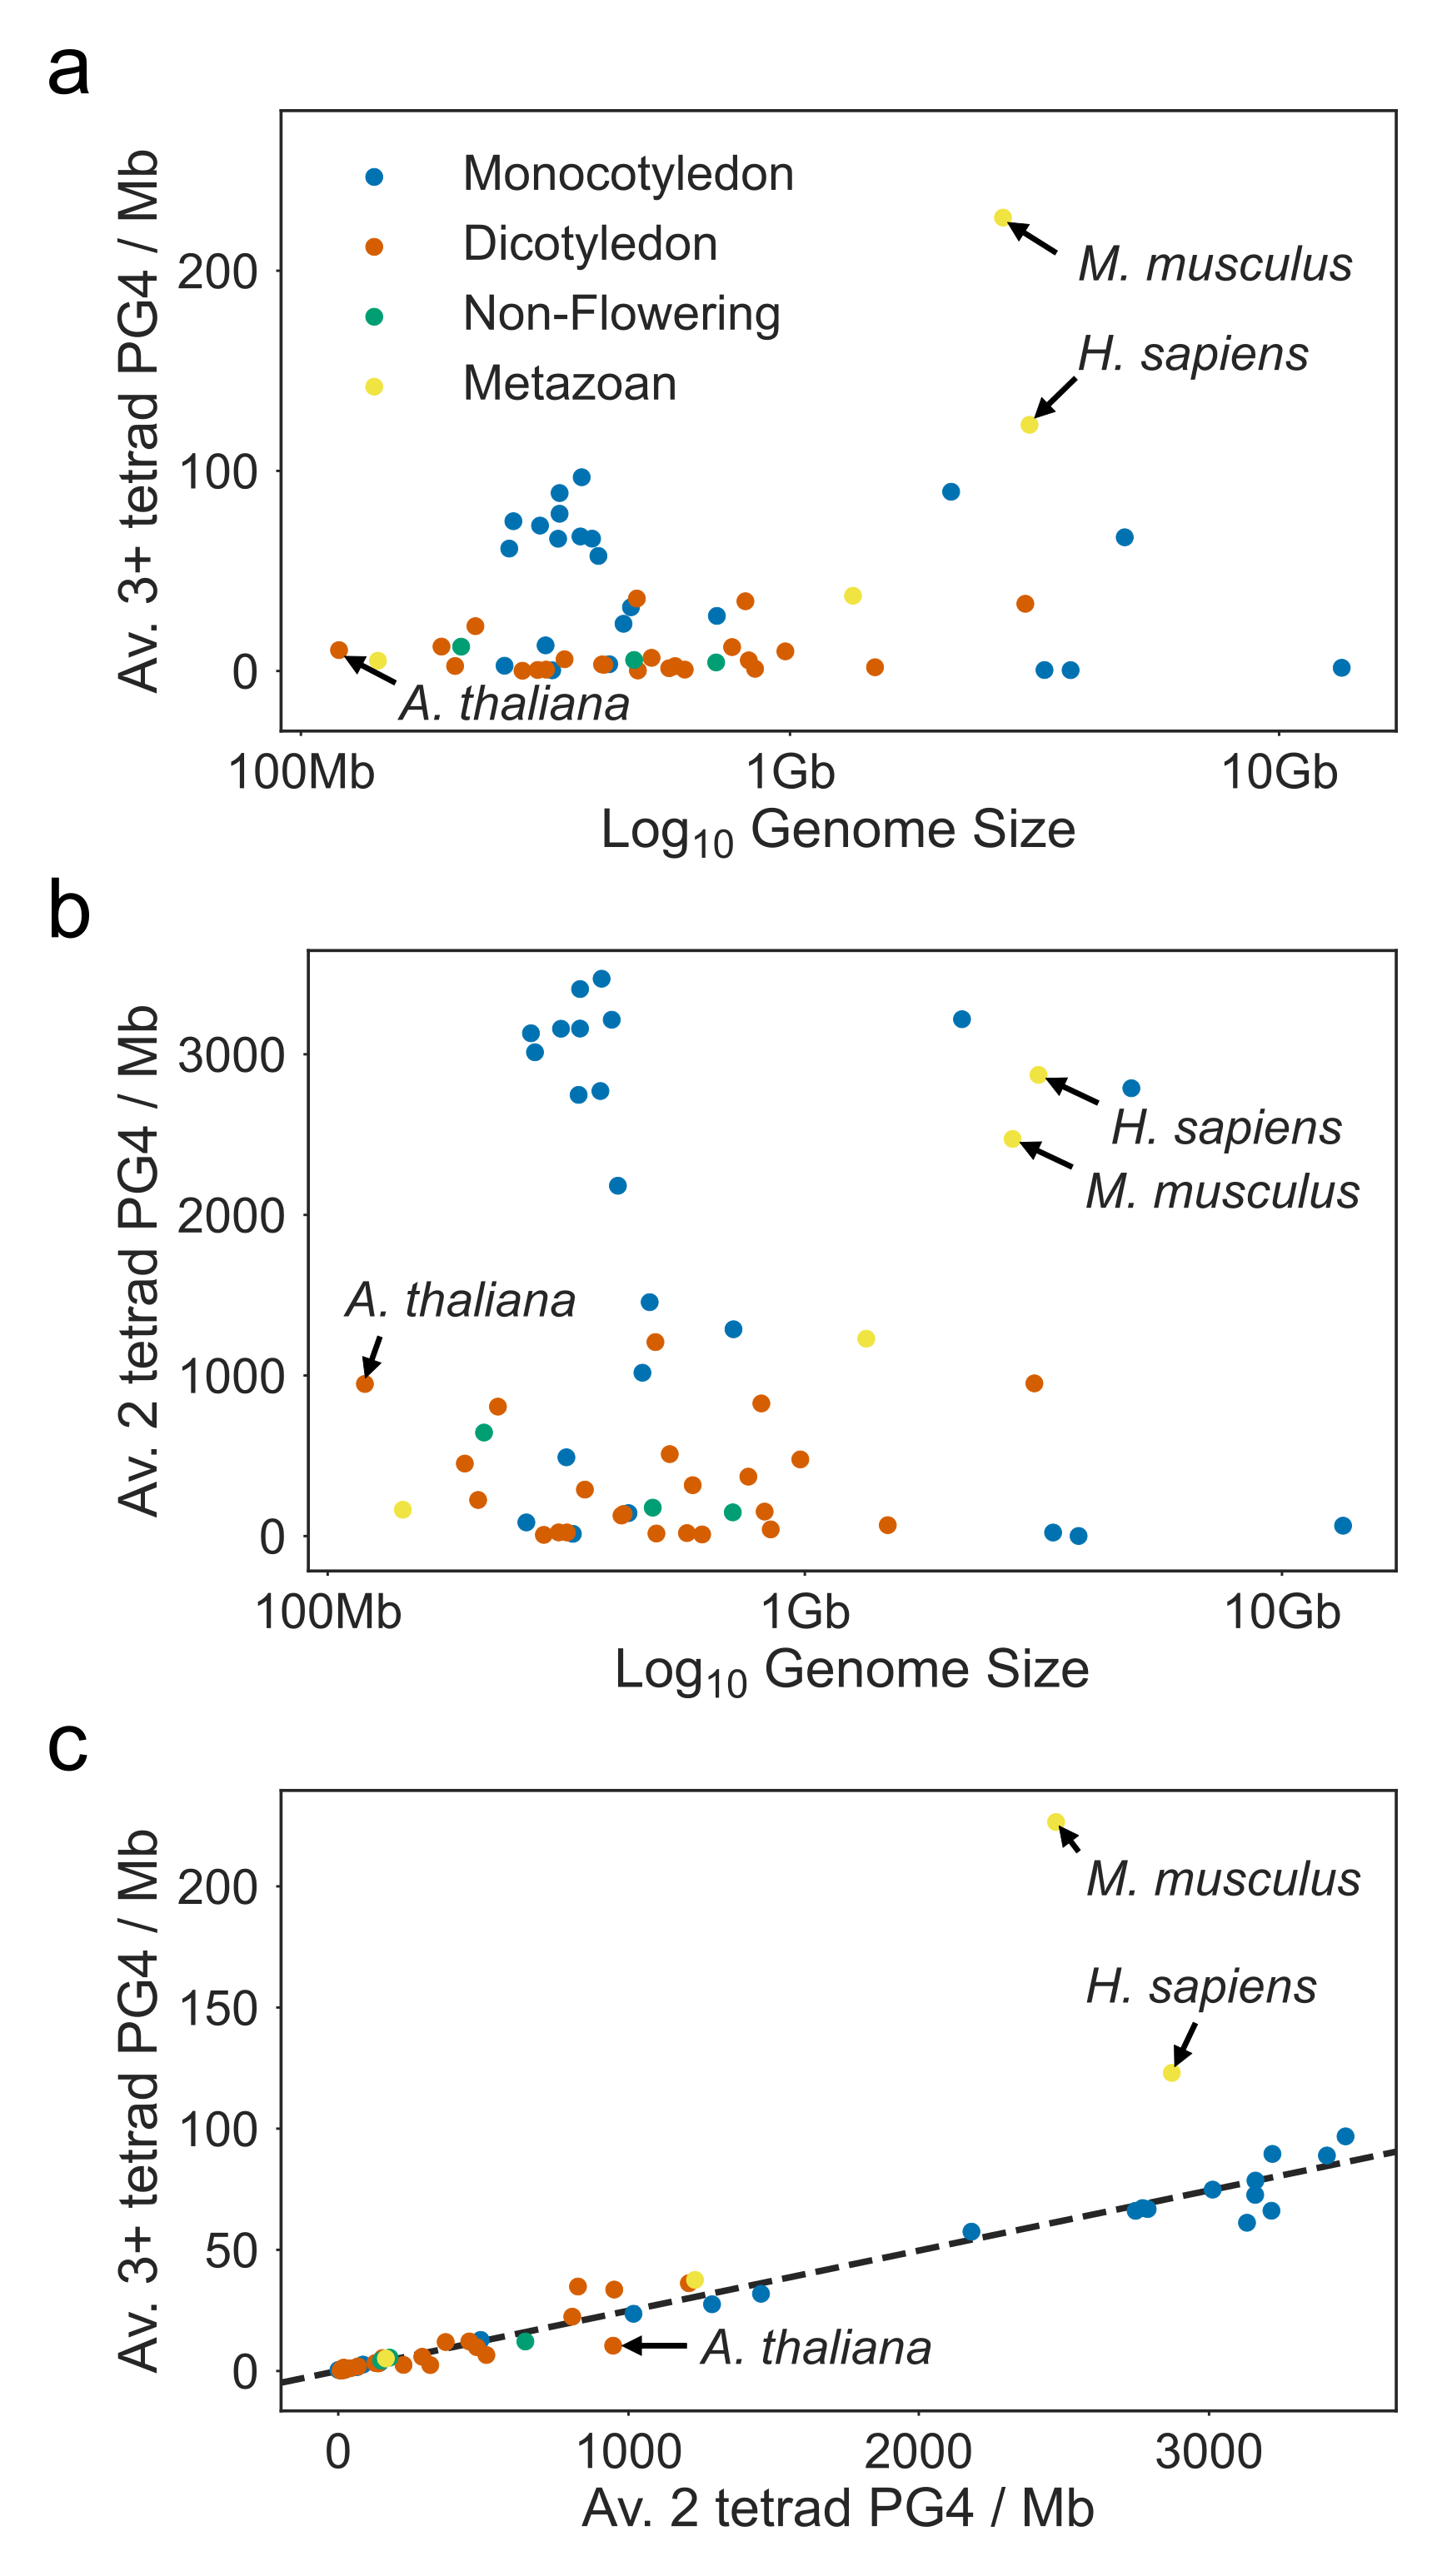
\includegraphics[width=\textwidth,height=562pt,keepaspectratio]{chapter_4/figures/pg4_density_plant_genomes.png}
\caption[PG4 density of Plant Genomes]{\textbf{PG4   density   of   Plant   Genomes}   \textbf{a)}   and   \textbf{b)}   Scatter   plots   showing   log10   genome   size   vs. the   average   \textbf{a)}   three   tetrad   or   more   and   \textbf{b)}   two   tetrad   PG4   density   per   Megabase   for   22   Monocotyledons,   21   Dicotyledons,   3   Non-flowering   plants   and   4   metazoans.   Plant   genomes   are   much   poorer   in   three   tetrad   PG4s   than   the   metazoans   \textit{H.   sapiens}   and   \textit{M.   musculus} ,   but   have   more   comparable   densities   of   two   tetrad   PG4s.   \textbf{c)}   Scatter   plot   showing   the   relationship   between   three   tetrad   and   two   tetrad   PG4   densities.   \textit{M.   musculus}   and   \textit{H.   sapiens}   do   not   follow   the   same   pattern   of   relative   PG4   densities   as   plants.   \label{pg4_genomes}}
\end{figure}

\newpage

\hypertarget{pg4s-are-non-uniformly-distributed-in-the-arabidopsis-thaliana-genome}{%
\subsection{\texorpdfstring{PG4s are non-uniformly distributed in the
\emph{Arabidopsis thaliana}
genome}{PG4s are non-uniformly distributed in the Arabidopsis thaliana genome}}\label{pg4s-are-non-uniformly-distributed-in-the-arabidopsis-thaliana-genome}}

It is well documented that PG4s are not randomly distributed in the
human genome, with an enrichment of PG4s in promoter sequences. We
therefore used metagene profiles to identify the localisation of PG4s in
the Arabidopsis genome. The distribution of G content (in 20bp windows),
two tetrad PG4s, and three or more tetrad PG4s was calculated and
averaged across all all protein coding genes. The density in UTRs and
CDS regions (including introns) was reinterpolated into 20 and 100 bins,
respectively, and an upstream and downstream size of 500bp was used.
PG4s identified on the coding and template strands were analysed
separately. The GC content of genic regions is greater than intergenic
sequence, with the greatest coding strand G content towards the TSS
distal end of the CDS, and the greatest template strand C content in the
5' UTR and at the TSS proximal end of the CDS (Fig \ref{metagene}a).
This translates into a greater density of two tetrad PG4s localised at
the beginning of genes on the template strand and towards the end of
genes on the coding strand (Fig \ref{metagene}c). The number of three or
more tetrad PG4s is extremely low in the Arabidopsis genome, however
there is a slight increase around the TSS and in the 5' UTR on the
template strand, and at the TSS distal end in the coding strand (Fig
\ref{metagene}b).

In order to identify whether these PG4s are simply a product of higher
local GC content in different genic regions, we performed simulation of
genomic sequence by shuffling in 20bp windows, maintaining the
nucleotide and dinucleotide contents. This does not change the GC
content distribution of the metagene profile. It does, however, indicate
a strong enrichment of two tetrad PG4s over expected levels throughout
the CDS, particularly on the template strand at the TSS proximal end
(Fig \ref{metagene}c). Furthermore, we see an enrichment of three or
more tetrad PG4s over expected levels around the TSS on the template
strand (Fig \ref{metagene}b), and a depletion inside coding regions on
both strands.

\newpage

\begin{figure}[htbp]
\centering
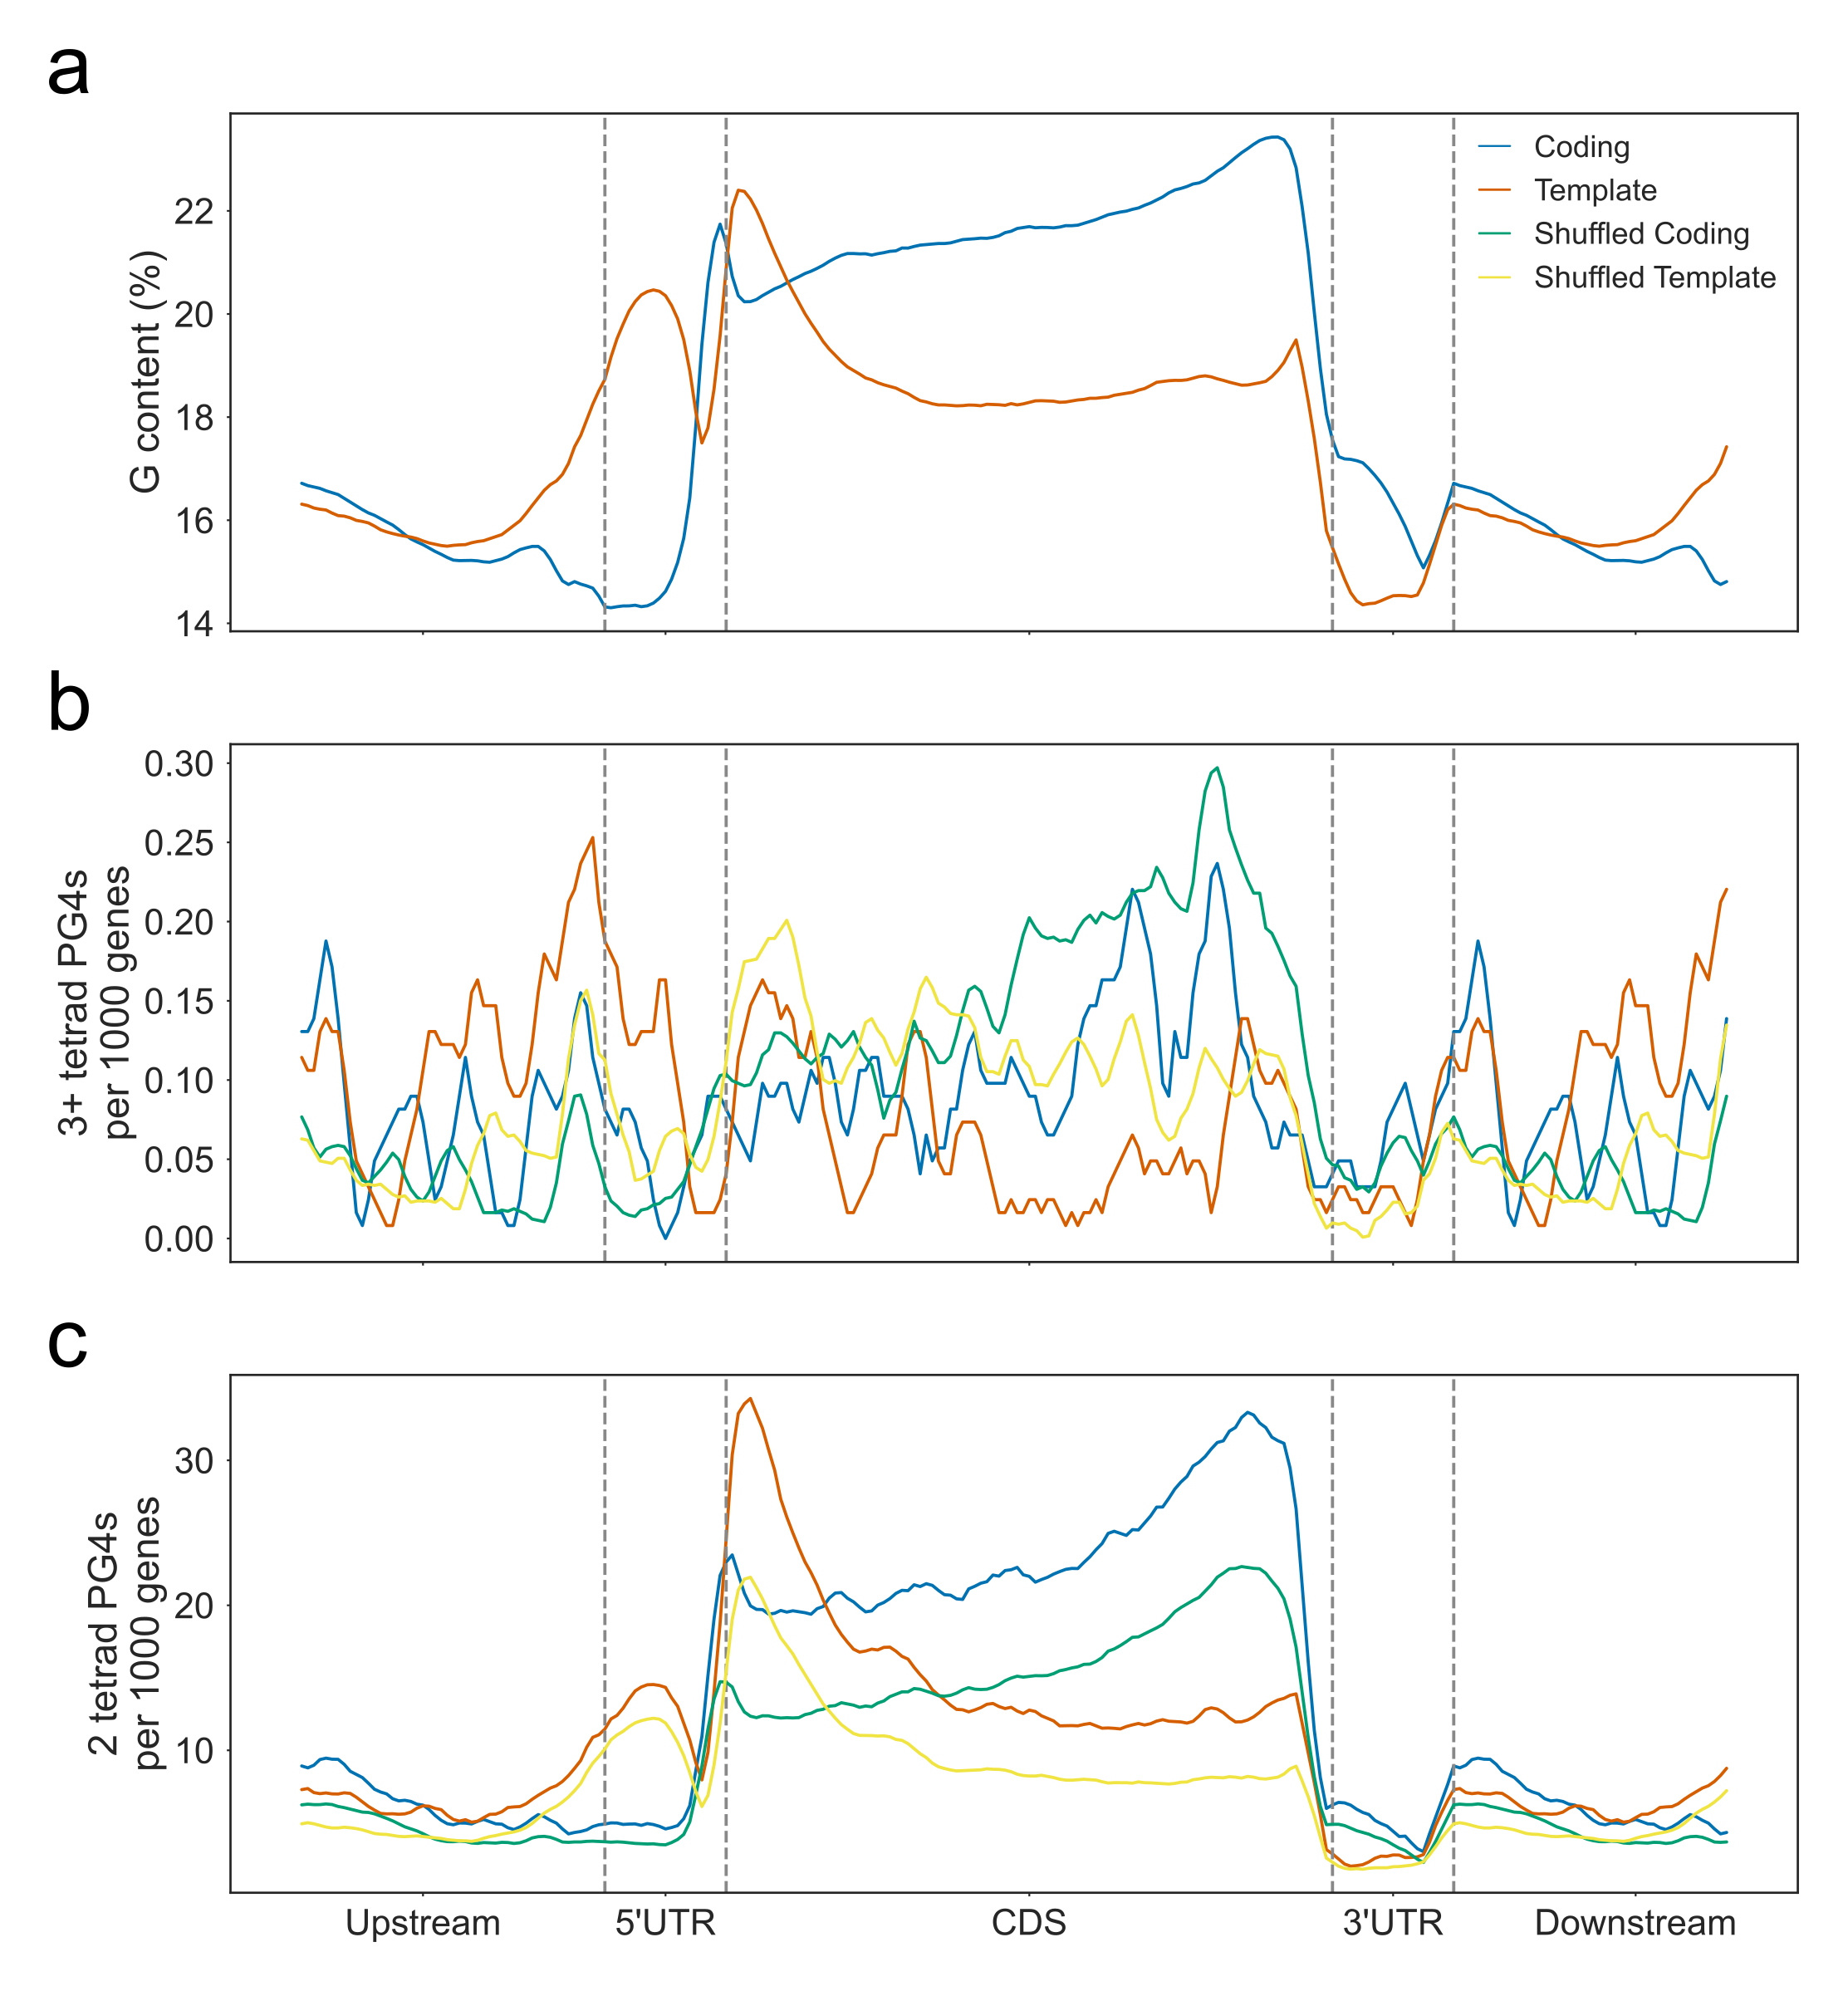
\includegraphics[width=\textwidth,height=562pt,keepaspectratio]{chapter_4/figures/gc_g4_content_metagene.png}
\caption[Metagene Profile of GC content and PG4 density]{\textbf{Metagene   Profile   of   GC   content   and   PG4   density}   Metagene   profiles   showing   the   \textbf{a)}   G   content,   \textbf{b)}   three   or   more   tetrad   PG4   content   and   \textbf{c)}   two   tetrad   PG4   content   of   protein   coding   genes   on   the   coding   (blue)   and   template   (orange)   strands.   Green   and   yellow   lines   show   the   average   coding   and   template   PG4   contents   for   genes   where   the   sequence   has   been   shuffled   in   20bp   windows,   maintaining   mononucleotide   and   dinucleotide   frequencies.   G   content   metaprofiles   are   identical   to   the   real   metaprofiles   in   these   shuffled   controls.   \label{metagene}}
\end{figure}

\newpage

\hypertarget{reverse-translation-permutation-testing-reveals-codon-usage-bias-towards-g4-formation-in-template-strand-5-utrs}{%
\subsection{Reverse translation permutation testing reveals codon usage
bias towards G4 formation in template strand 5'
UTRs}\label{reverse-translation-permutation-testing-reveals-codon-usage-bias-towards-g4-formation-in-template-strand-5-utrs}}

The enrichment of two tetrad PG4s inside coding regions in Arabidopsis
could be indicative of a function for G4s in transcriptional or
translational regulation, however, it is also possible that these
sequences could be a byproduct of specific protein motifs which are
encoded by GC rich codons. In order to explore this, we developed a
novel sequence permutation method which we call ``reverse translation''.
First, we calculated the codon usage table (the quantifiable bias in
usage of synonymous codons) from all CDS sequences. The sequences were
then translated into their protein product sequence, then reverse
translated back into potential coding sequences (PCSs) with randomly
selected codons, but using the codon usage table as weights. These PCSs
are therefore sequences which might be expected to code for the given
protein, assuming that the codon bias is identical across all genes and
all positions in genes. We performed 100 reverse translation shufflings
for each CDS and then calculated the GC and PG4 content of each PCS
using the Quadparser method and G4Seeqer.

The GC content of CDSs is greatest towards the start and end of the
interval, and dips in the middle (Fig \ref{revtrans}a). This is due to a
greater G content at the start codon proximal end on the template
strand, and a greater G content at the start codon distal end on the
coding strand. When we performed reverse translation using a single
codon usage table, some of this bias was abolished. This indicates that
most of the GC content of the CDS is not hardcoded into the sequence by
the protein content. Codon usage is therefore presumably different at
the start and end of the gene.

As shown in Fig \ref{metagene}c, there is a higher density of PG4s at
the start of the CDS on the template strand, and a higher density
towards the end of the CDS on the coding strand. This is also seen in
Fig \ref{revtrans}b \& c. PCS sequences demonstrate the same biases in
PG4 distribution using both Quadparser and G4Seeqer predictions. This
demonstrates that unlike GC content, the PG4 content of some genes is
hardcoded by protein sequence (Fig \ref{revtrans}b \& c). This may be
due to the repetitive nature of some protein motifs. PCS PG4 content is
higher than the real PG4 levels across the coding strand however,
suggesting that codons which reduce PG4 forming potential on this strand
may be selected for. On the template strand, we see strong enrichment of
PG4s in real sequences over expected levels from PCSs in the first 50\%
of the CDS (Fig \ref{revtrans}b \& c). This suggests that C rich codons
may be selected for at the start of genes to increase the G4 forming
potential of the template strand. We wondered whether CDS G4s might be
selected for in genes which have short 5' UTRs which might not be able
to contain G4s, however we did not see any correlation between the
length of 5' UTRs and the presence of G4s in the first 100bp of CDS
regions (Spearmans rho 0.014).

\newpage

\begin{figure}[htbp]
\centering
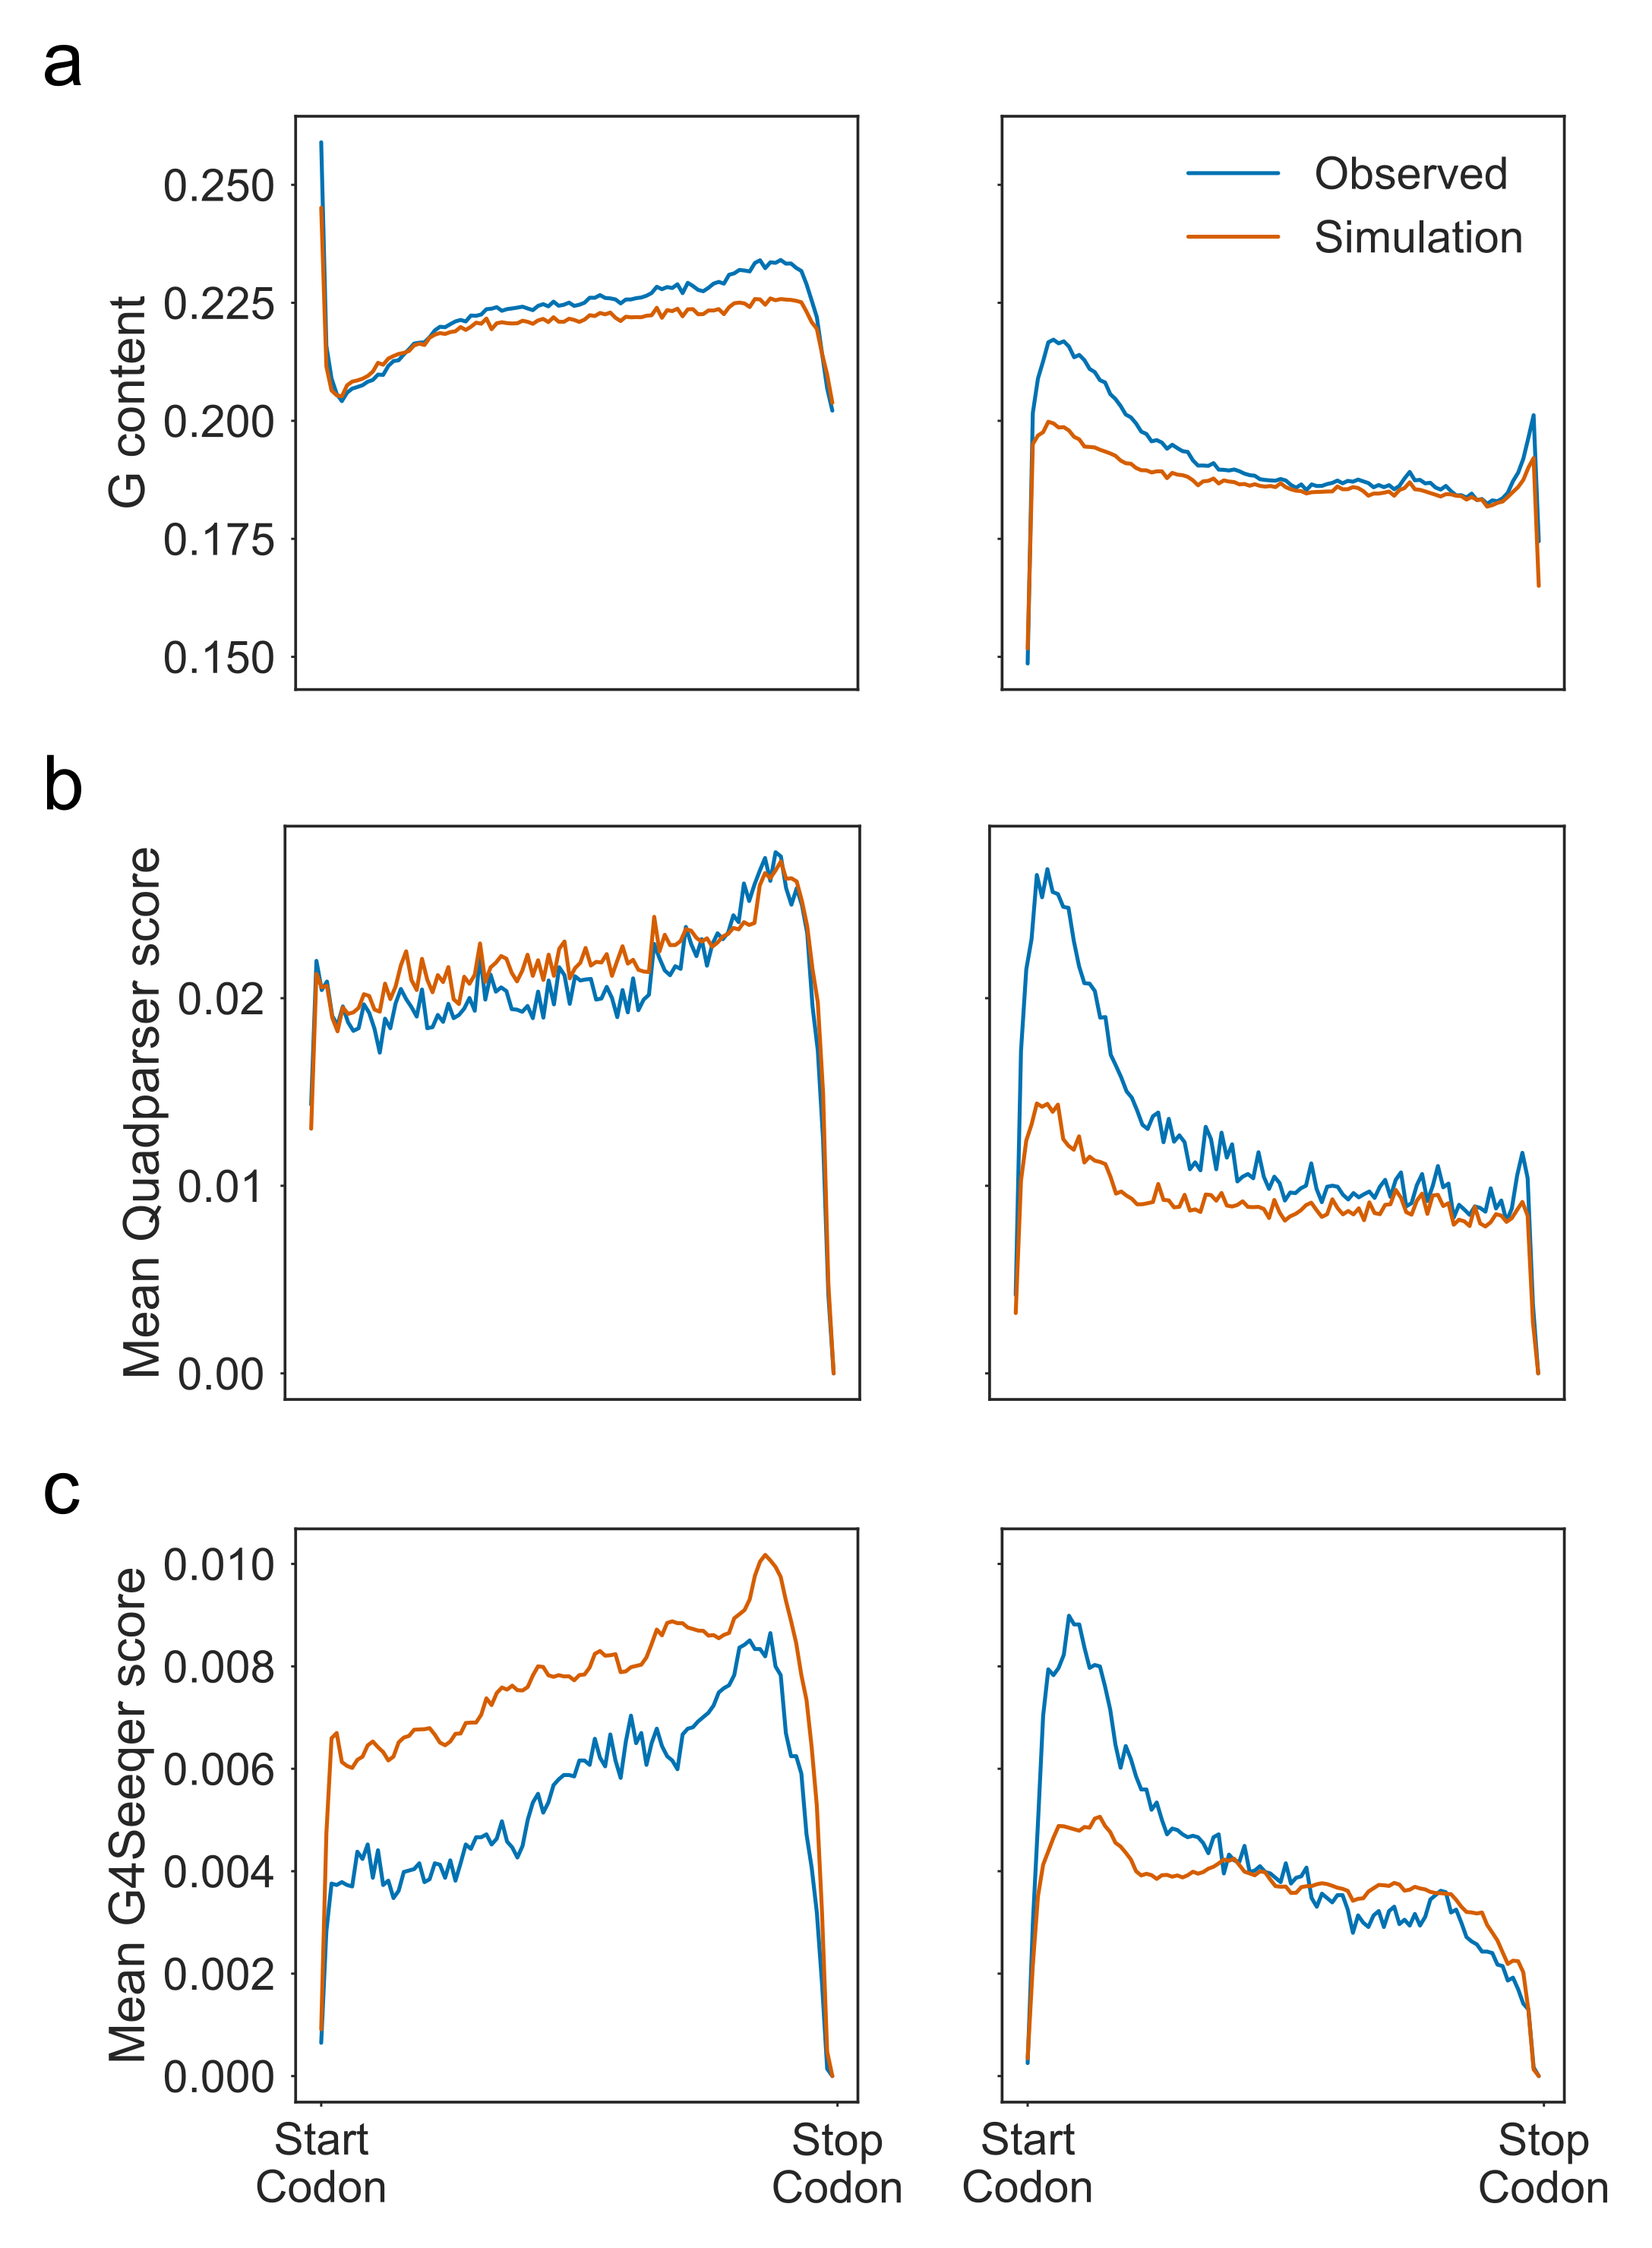
\includegraphics[width=\textwidth,height=562pt,keepaspectratio]{chapter_4/figures/reverse_translation.png}
\caption[Reverse Translation Simulation shows that PG4s are enriched at the Start Codon proximal region of the template strand.]{\textbf{Reverse   Translation   Simulation   shows   that   PG4s   are   enriched   at   the   Start   Codon   proximal   region   of   the   template   strand.}   Metagene   profiles   showing   \textbf{a)}   G   content   \textbf{b)}   Quadparser   PG4s   and   \textbf{c)}   G4Seeqer   PG4s   for   real   CDS   regions   (blue)   vs. reverse   translation   simulated   potential   coding   sequences   (PCS)   (orange).   \label{revtrans}}
\end{figure}

\newpage

\hypertarget{protein-motifs-hardcode-g4-forming-potential-into-coding-regions}{%
\subsection{Protein motifs hardcode G4 forming potential into coding
regions}\label{protein-motifs-hardcode-g4-forming-potential-into-coding-regions}}

Our reverse translation method indicates that the PG4 forming potential
of may arise from protein sequence, i.e.~if protein sequence is
evolutionarily constrained, then PG4s are hardcoded into the CDS. We
performed an analysis of which protein motifs most often lead to two
tetrad PG4s. All overlapping PG4s and the G-runs that form them were
predicted, and the amino acids which are encoded by each G-run was
identified. The G-run was then classified as either hardcoded or not,
depending on whether or not the same amino acids could be encoded
differently without introducing a G-run in the same position. We also
identified repetitive and non-repetitive G-runs. G-runs were considered
repetitive if the protein motifs that they encode were the same for all
G-runs in the G4.

Our analysis shows that 58\% of PG4 G-runs on the coding strand, and
48\% on the template strand, are hardcoded. Of these hardcoded PG4s,
around 51\% and 60\% are found in repetitive PG4s on the coding and
template strand, respectively. On the other hand, most non-hardcoded
PG4s on both strands are also non-repetitive (Fig \ref{hardcoded}a).
This suggests the presence of a number of entirely hardcoded PG4s which
are encoded by repetitive protein motifs.

We counted the total number of hardcoded G-runs in each overlapping PG4
register on both strands (Fig \ref{hardcoded}b). We found that on both
strands, the greatest number of PG4s were completely hardcoded, again
suggesting a large number of PG4s encoded by repetitive protein motifs.
On the template strand, however, we also found that 19\% of PG4s had no
G-runs hardcoded, suggesting the presence of template PG4s which are
selected for specifically.

Analysis of the frame of the first G in G-runs vs.~their hardcoded
status identifies that 46\% and 48\% of coding and template G-runs in
PG4s are frame 0, i.e.~are made up of the first two bases of a codon.
These are all hardcoded. This is intuitive since the third position of
codons is the ``wobble'' position which is most often degenerate amongst
synonymous codons. Approximately one third and one fifth of coding
strand G-runs in frames 1 and 2 are hardcoded, whilst all template
strand G-runs in frames 1 and 2 are not hardcoded. Interestingly, 36\%
of G-runs on the coding strand are frame 2 whilst only 24\% on the
template strand are. This is most likely due to the relative frequencies
of different amino acids whose codons may form G-runs.

\newpage

\begin{figure}[htbp]
\centering
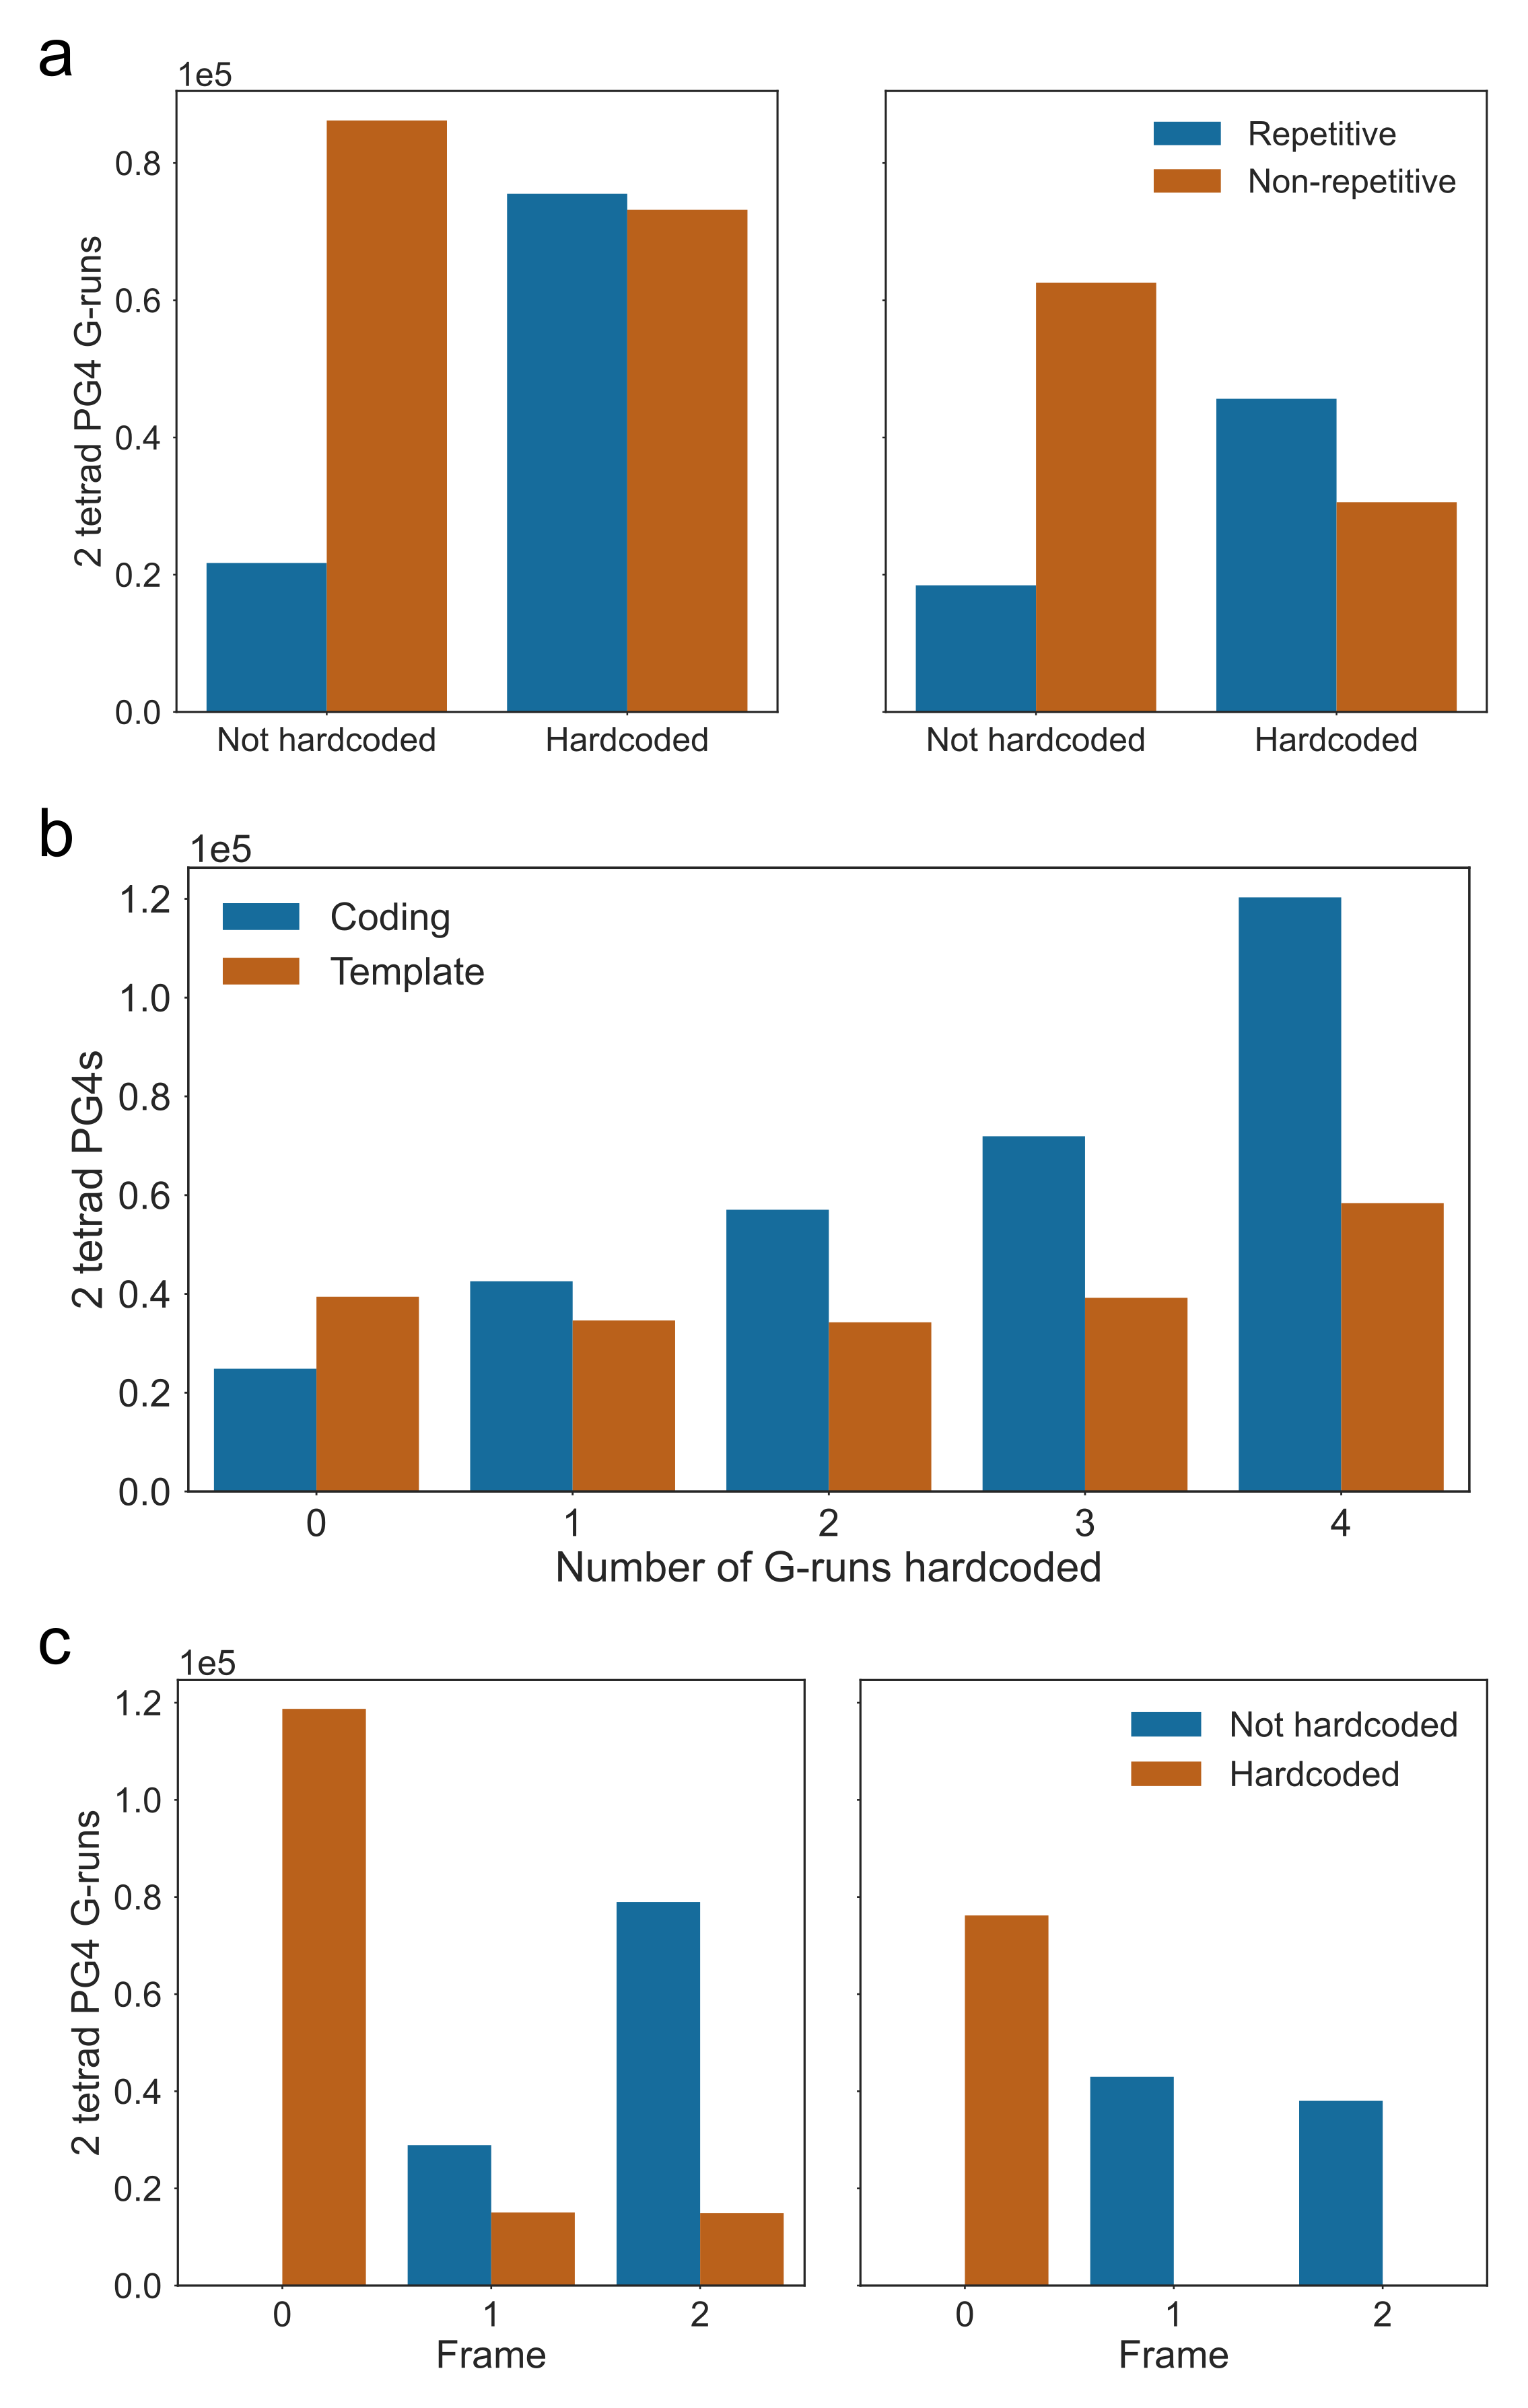
\includegraphics[width=\textwidth,height=562pt,keepaspectratio]{chapter_4/figures/pg4_g_run_hardcoded_freq.png}
\caption[54\% of CDS PG4 G-runs are hardcoded by protein sequence.]{\textbf{54\%   of   CDS   PG4   G-runs   are   hardcoded   by   protein   sequence.}   \textbf{a)}   Frequency   plot   showing   the   total   number   of   G-runs   contributing   to   PG4s   which   are   hardcoded   and   repetitive.   Left   and   right   panels   show   frequencies   on   coding   and   template   strands,   respectively.   Hardcoded   G-runs   are   defined   as   those   GG   dinucleotides   that   cannot   be   removed   from   the   sequence   without   changing   the   amino   acid   sequence   which   is   coded   for.   Repetitive   G-runs   are   defined   as   those   which   contribute   to   PG4s   where   all   G-runs   are   part   of   codons   which   encode   the   same   sequence.   \textbf{b)}   Frequency   plot   showing   the   total   number   of   hardcoded   G-runs   for   each   overlapping   PG4   register   on   the   coding   (blue)   and   template   (orange)   strands,   respectively.   \textbf{c)}   Frequency   plots   showing   start   frame   of   CDS   G-runs   vs. hardcoded   status.   Left   and   right   panels   show   frequencies   on   coding   and   template   strands,   respectively.   \label{hardcoded}}
\end{figure}

\newpage

To identify the location of these non-hardcoded template PG4s in the
CDS, we plotted metagene profiles (Fig \ref{hc_metagene}). We found that
on the coding strand, non-hardcoded PG4 levels were approximately the
same throughout CDSs (mean 7.7\%, standard deviation 1.84\%) (Fig
\ref{hc_metagene}a). On the template strand however, the average
non-hardcoded PG4 levels on the template strand is 17\%, with a standard
deviation of 7\%. We found that 27\% of PG4s in first 10\% of the
metagene profile downstream of the start codon were completely
non-hardcoded (Fig \ref{hc_metagene}b). This shows that PG4s are
selected by codon usage in the start codon proximal region of the
template strand.

\newpage

\begin{figure}[htbp]
\centering
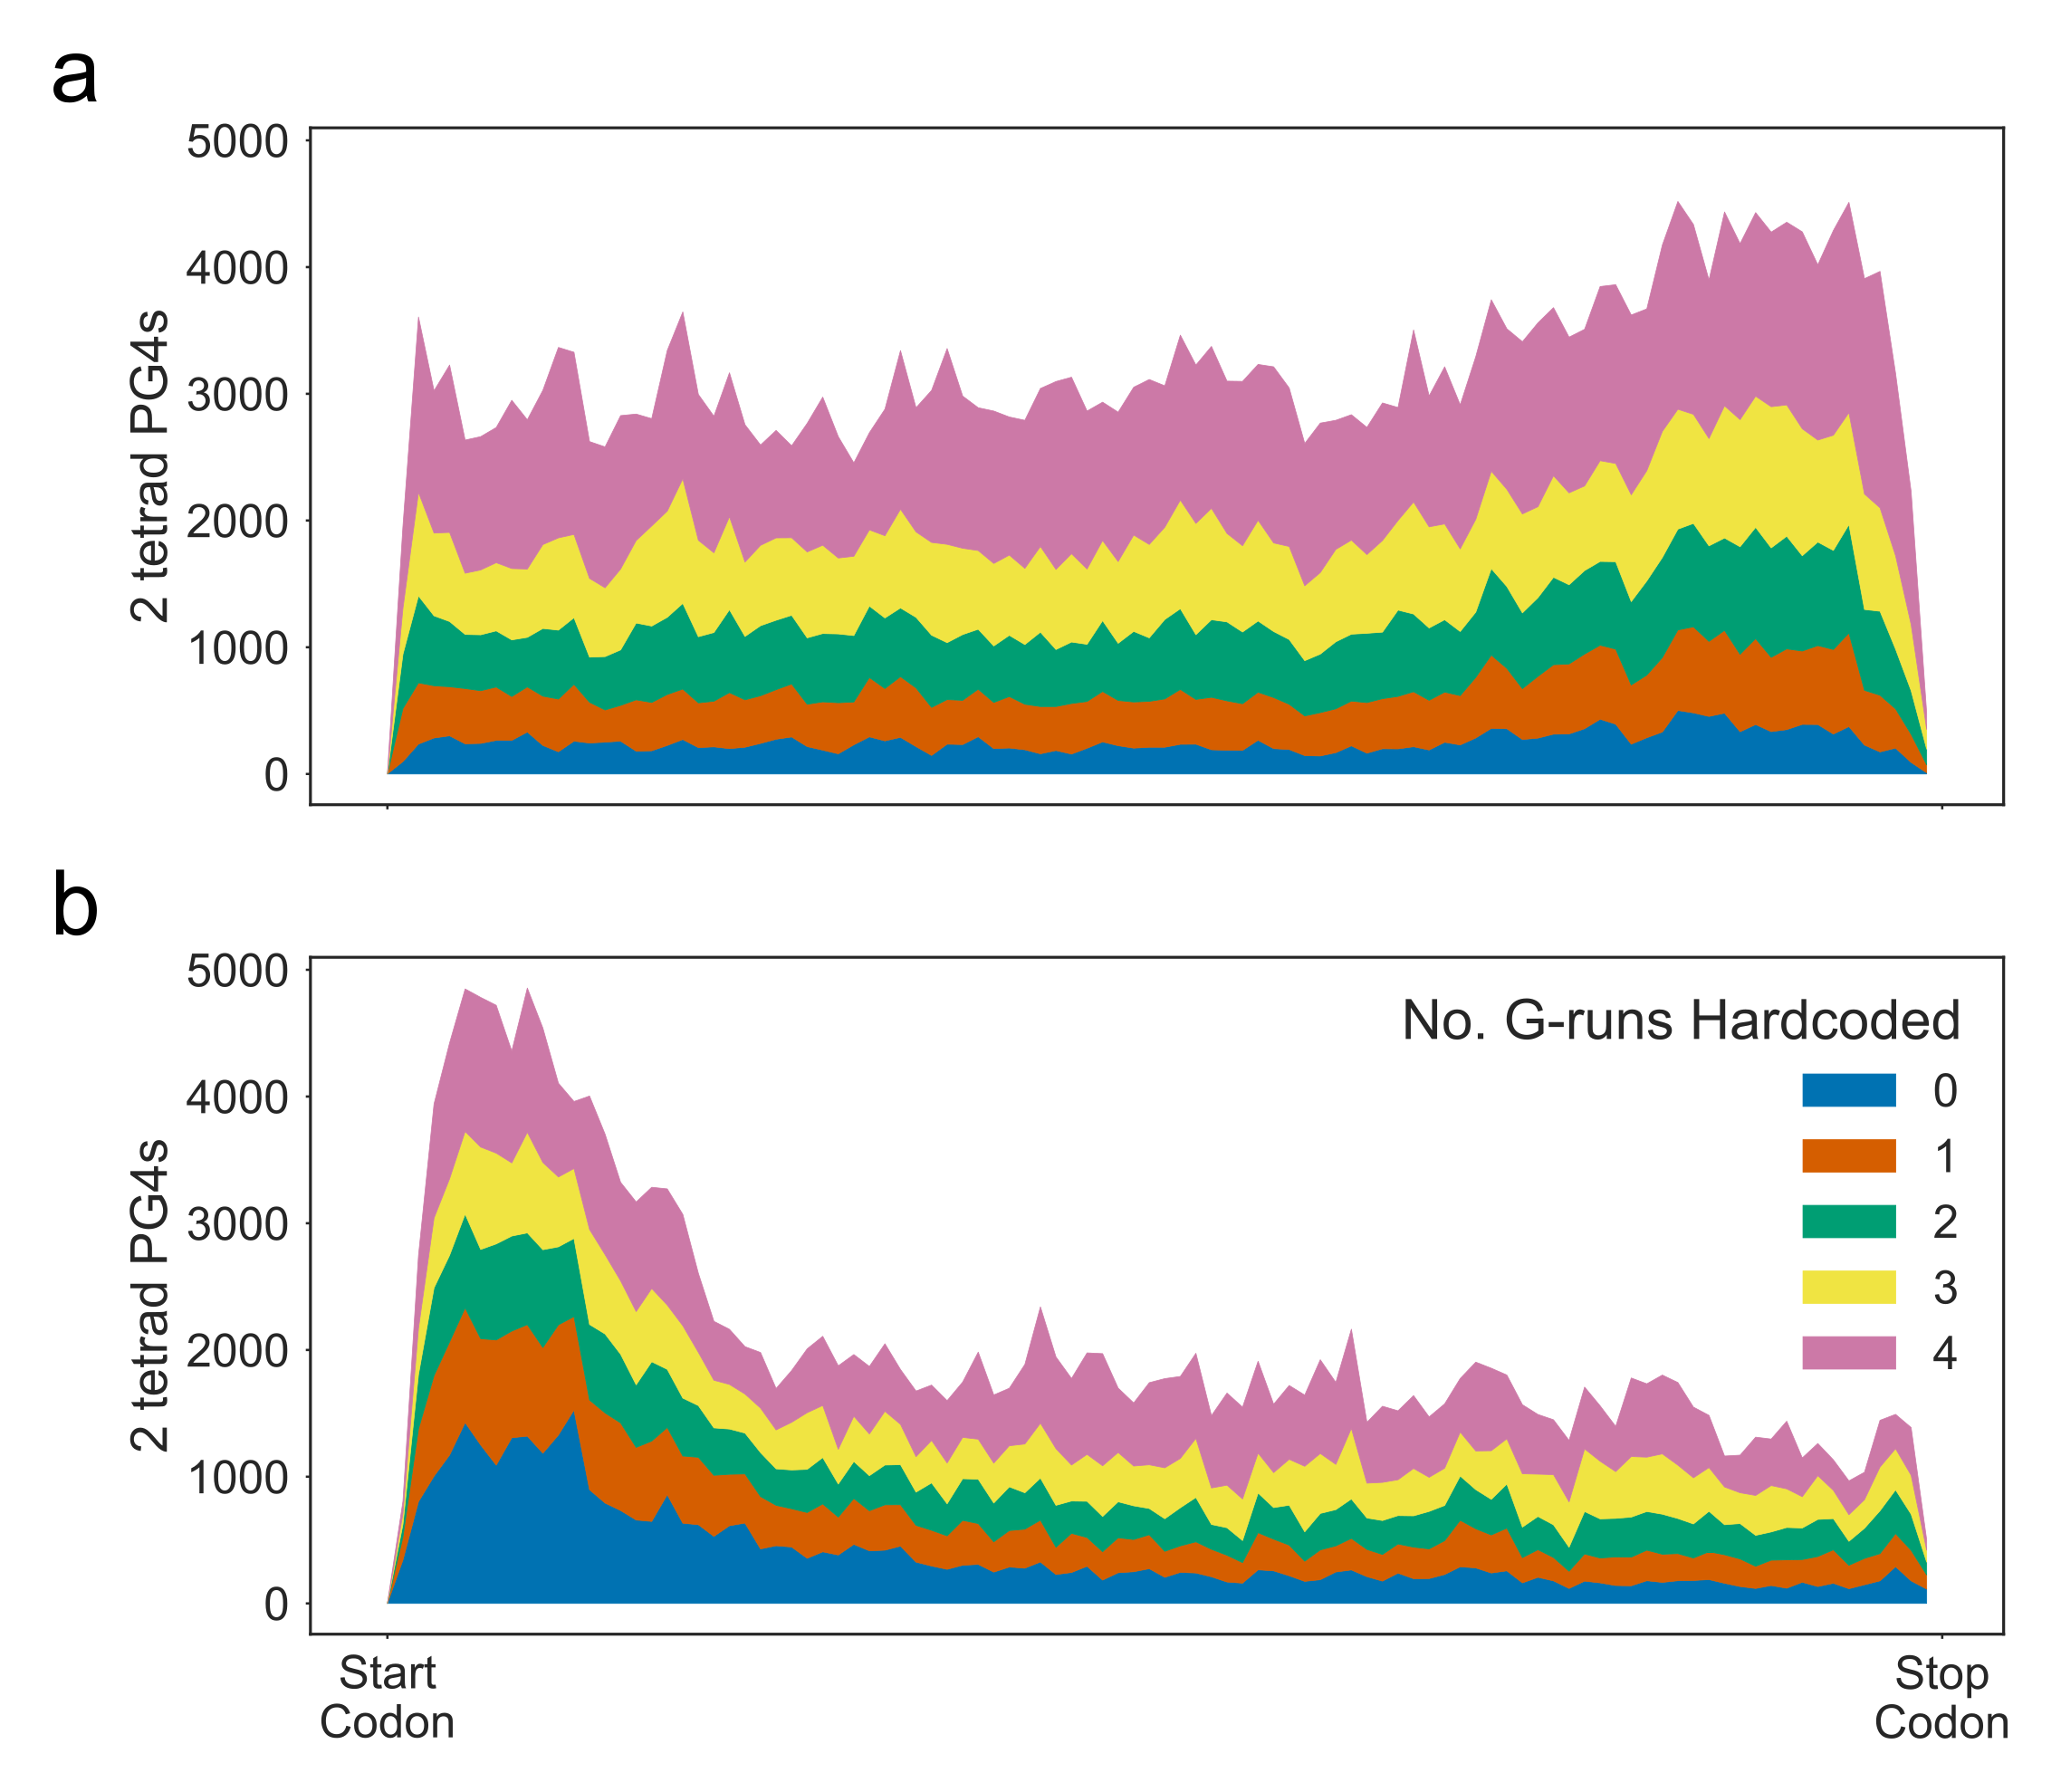
\includegraphics[width=\textwidth,height=562pt,keepaspectratio]{chapter_4/figures/cds_hardcoded_metagene.png}
\caption[Non-hardcoded PG4s levels are greater at the start codon proximal region of CDSs, on the template strand.]{\textbf{Non-hardcoded   PG4s   levels   are   greater   at   the   start   codon   proximal   region   of   CDSs,   on   the   template   strand.}   \textbf{a)}   Cumulative   metagene   profiles   showing   the   distribution   of   PG4s   with   different   numbers   of   hardcoded   G-runs   on   the   \textbf{a)}   coding   and   \textbf{b)}   template   strands,   respectively.   \label{hc_metagene}}
\end{figure}

\newpage

Harkness \& Mittermaier showed that sequences which are able to form a
variety of G4s through combinatorial interactions of greater than four
G-runs are more entropically favourable, and therefore higher melting
temperatures (Harkness and Mittermaier, 2016). Different PG4 registers
can be formed in sequences where there are extra Guanines in some
G-runs, allowing ``sliding'' (Harkness and Mittermaier, 2016), or where
there are five or more G-runs in close proximity, where G4s could be
formed from any four G-runs. We were interested to see whether template
strand PG4s at the start codon proximal end of CDSs tended to have more
registers, which might make them more stable. We therefore identified
all overlapping PG4 register clusters using network analysis (Figure
\ref{g4netx}a), and produced metagene profiles for clusters with only 1,
2-5, 6-20, or greater than 20 registers. We found that 64\% of PG4
clusters on both the coding and template strands of CDSs had greater
than one register. The largest number of registers for a single cluster
was 3096. This cluster was made up of 329 two base G-runs and was able
to form a maximum of 75 non-overlapping PG4s. To identify whether the
number of G-registers formed by PG4 clusters varied by CDS position, we
binned PG4s into metagene profiles (Figure \ref{g4netx}b). We did not
find much variation in the percentage of PG4s with G-register number
greater than one, on either strand, however (mean 64\%, standard
deviation 3.5\% for both strands).

\newpage

\begin{figure}[htbp]
\centering
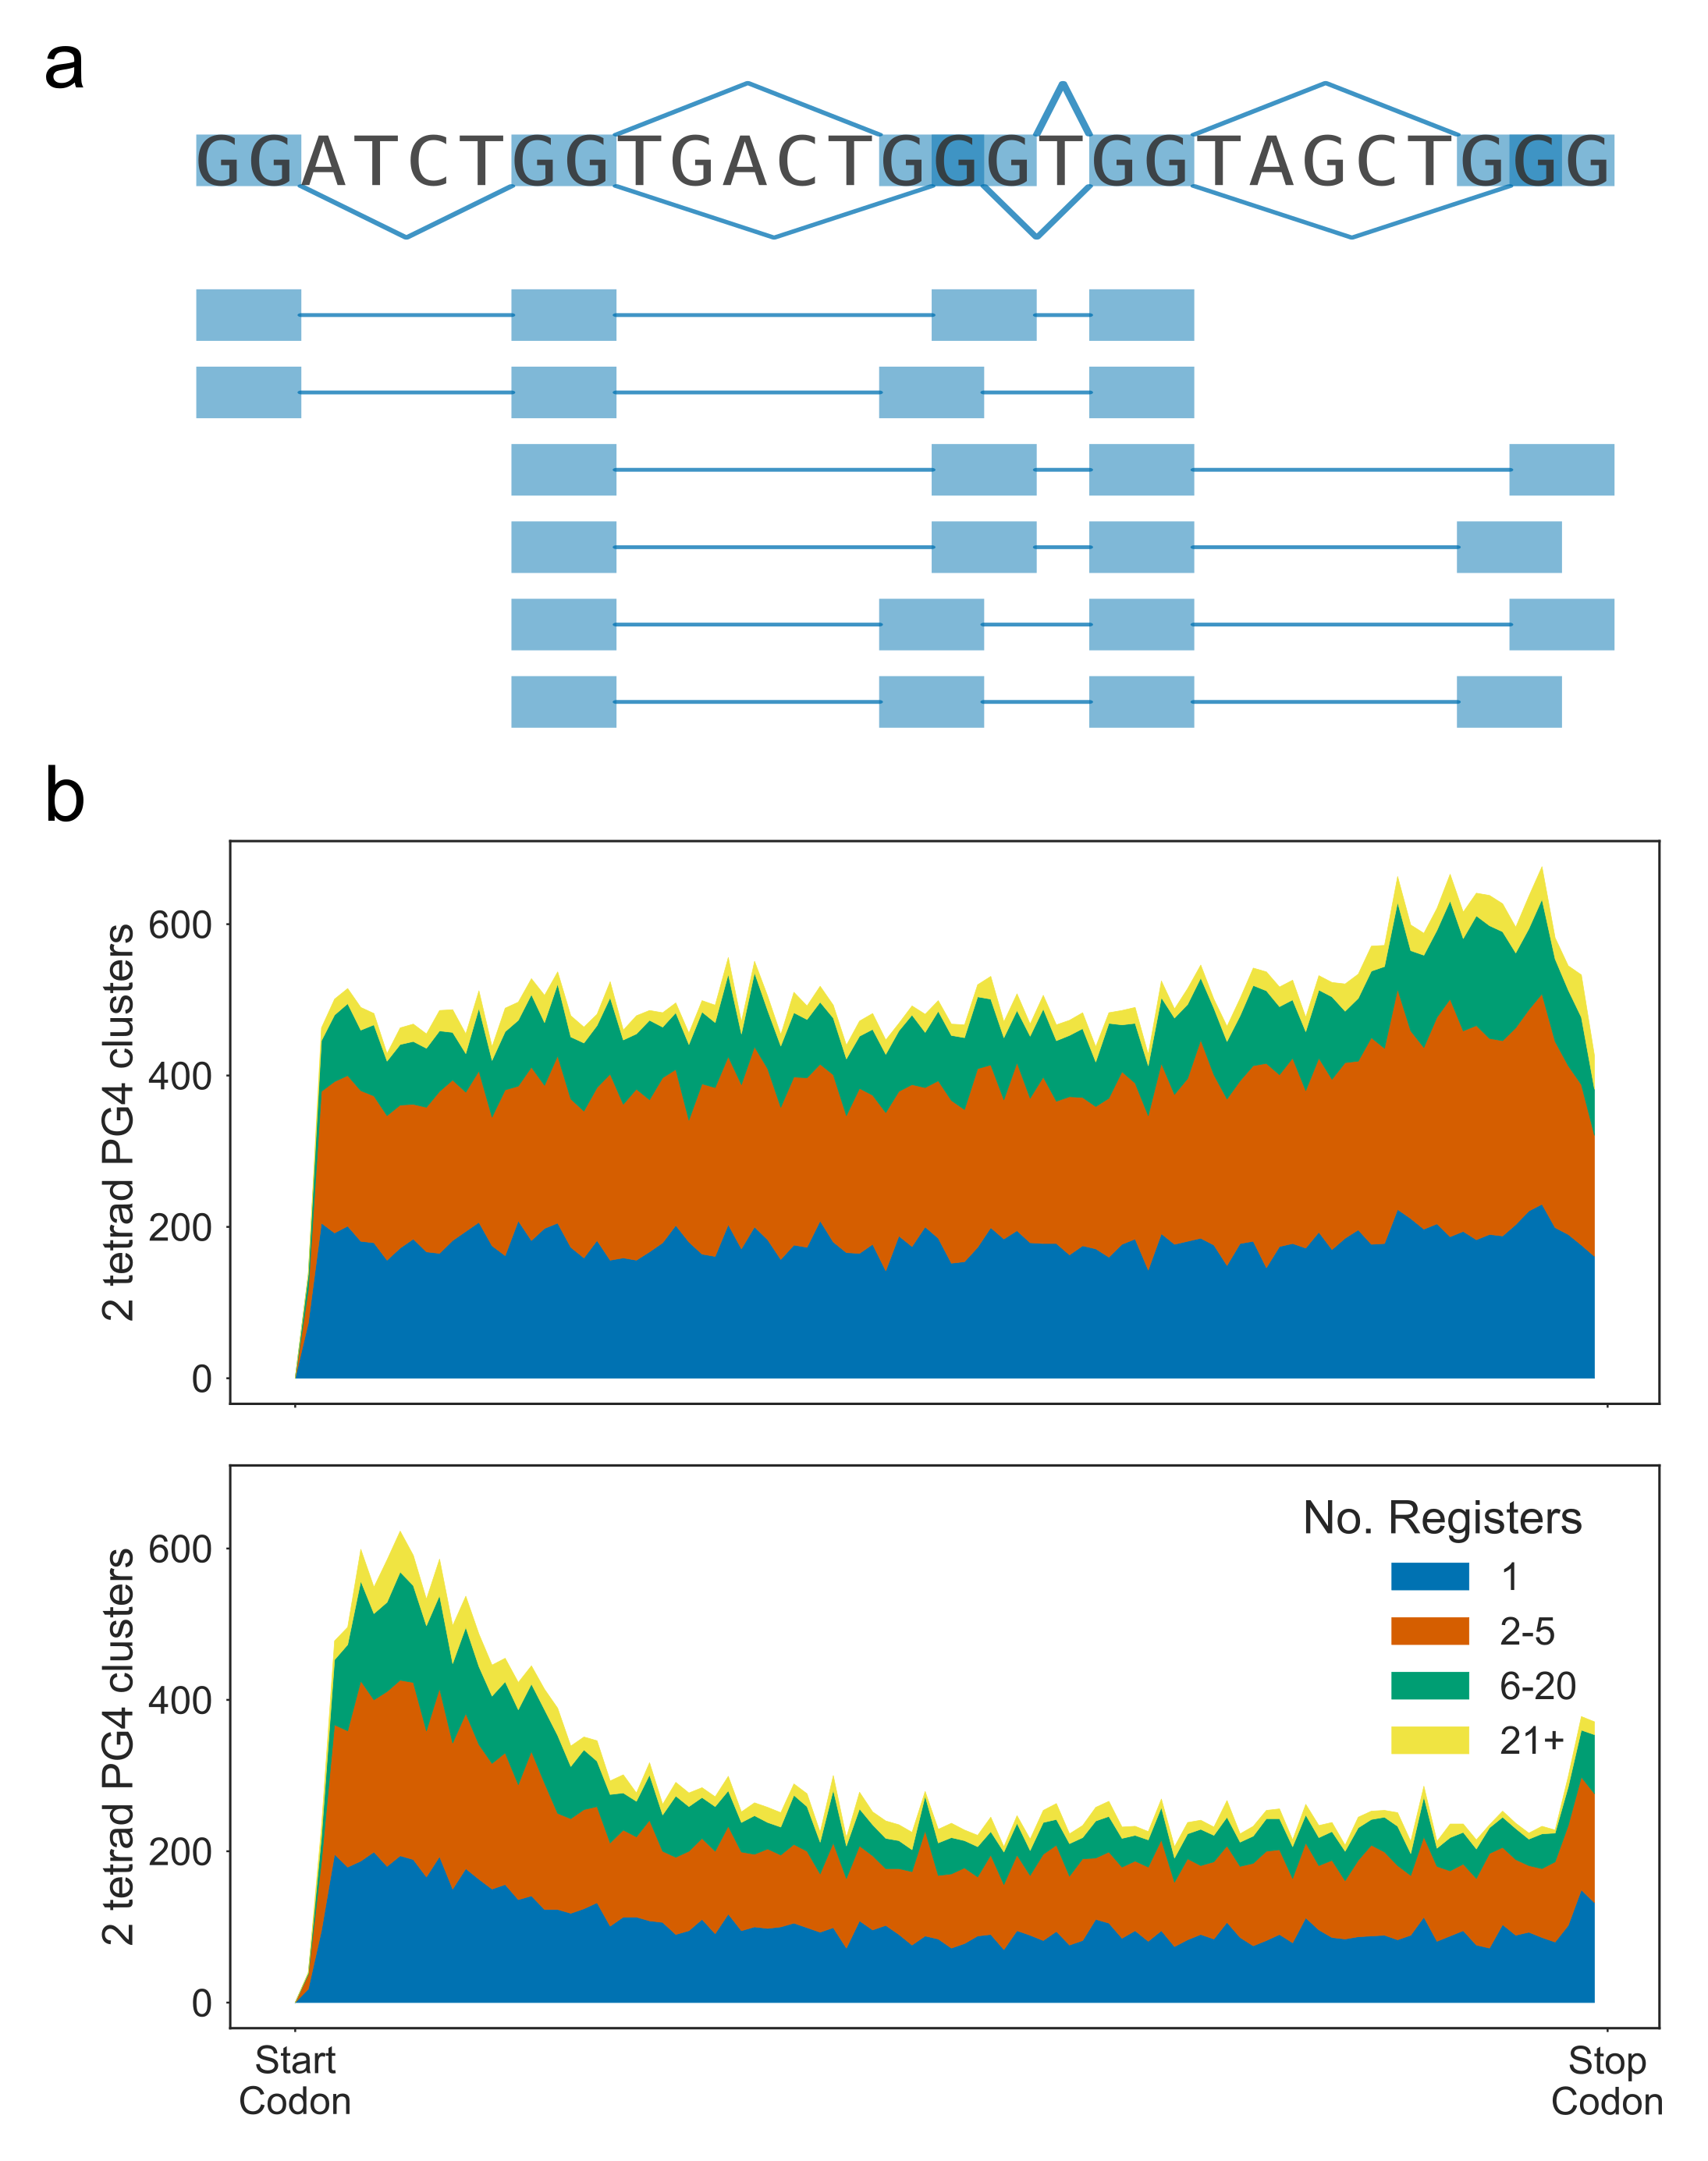
\includegraphics[width=\textwidth,height=562pt,keepaspectratio]{chapter_4/figures/pg4_register.png}
\caption[PG4 Register does not vary over CDSs]{\textbf{PG4   Register   does   not   vary   over   CDSs}   \textbf{a)}   Diagram   showing   how   a   sequence   with   multiple   G-runs   can   form   multiple   overlapping   PG4   registers   and   topologies.   \textbf{b)}   Cumulative   metagene   profiles   showing   distribution   of   PG4   clusters   with   different   numbers   of   PG4   registers   on   the   coding   strand   (top   panel)   and   template   strand   (bottom   panel).   \label{g4netx}}
\end{figure}

\newpage

Finally, we examined which amino acid motifs were most common in PG4
G-runs. We found that on the coding strand, by far the most common G-run
motif was glycine (Fig \ref{protmotif}). The majority of these G-runs
are hardcoded, because the codon for glycine is GGN (Fig
\ref{protmotif}a, left panel). Furthermore, more than 50\% of glycine
G-runs are found in repetitive PG4s, suggesting that poly-glycine is a
common PG4 forming motif (Fig \ref{protmotif}b). There was not a clear
majority motif for non-hardcoded PG4 G-runs.

On the template strand, we found that the most common PG4 G-run motif
was proline. This is again mostly hardcoded, since the codon for proline
is CCN (Fig \ref{protmotif}a, right panel). More than 50\% of proline
G-runs were also found in repetitive PG4s, suggesting that like glycine
on the coding strand, proline homopolymers are the most common PG4
forming motif on the template strand.

\newpage

\begin{figure}[htbp]
\centering
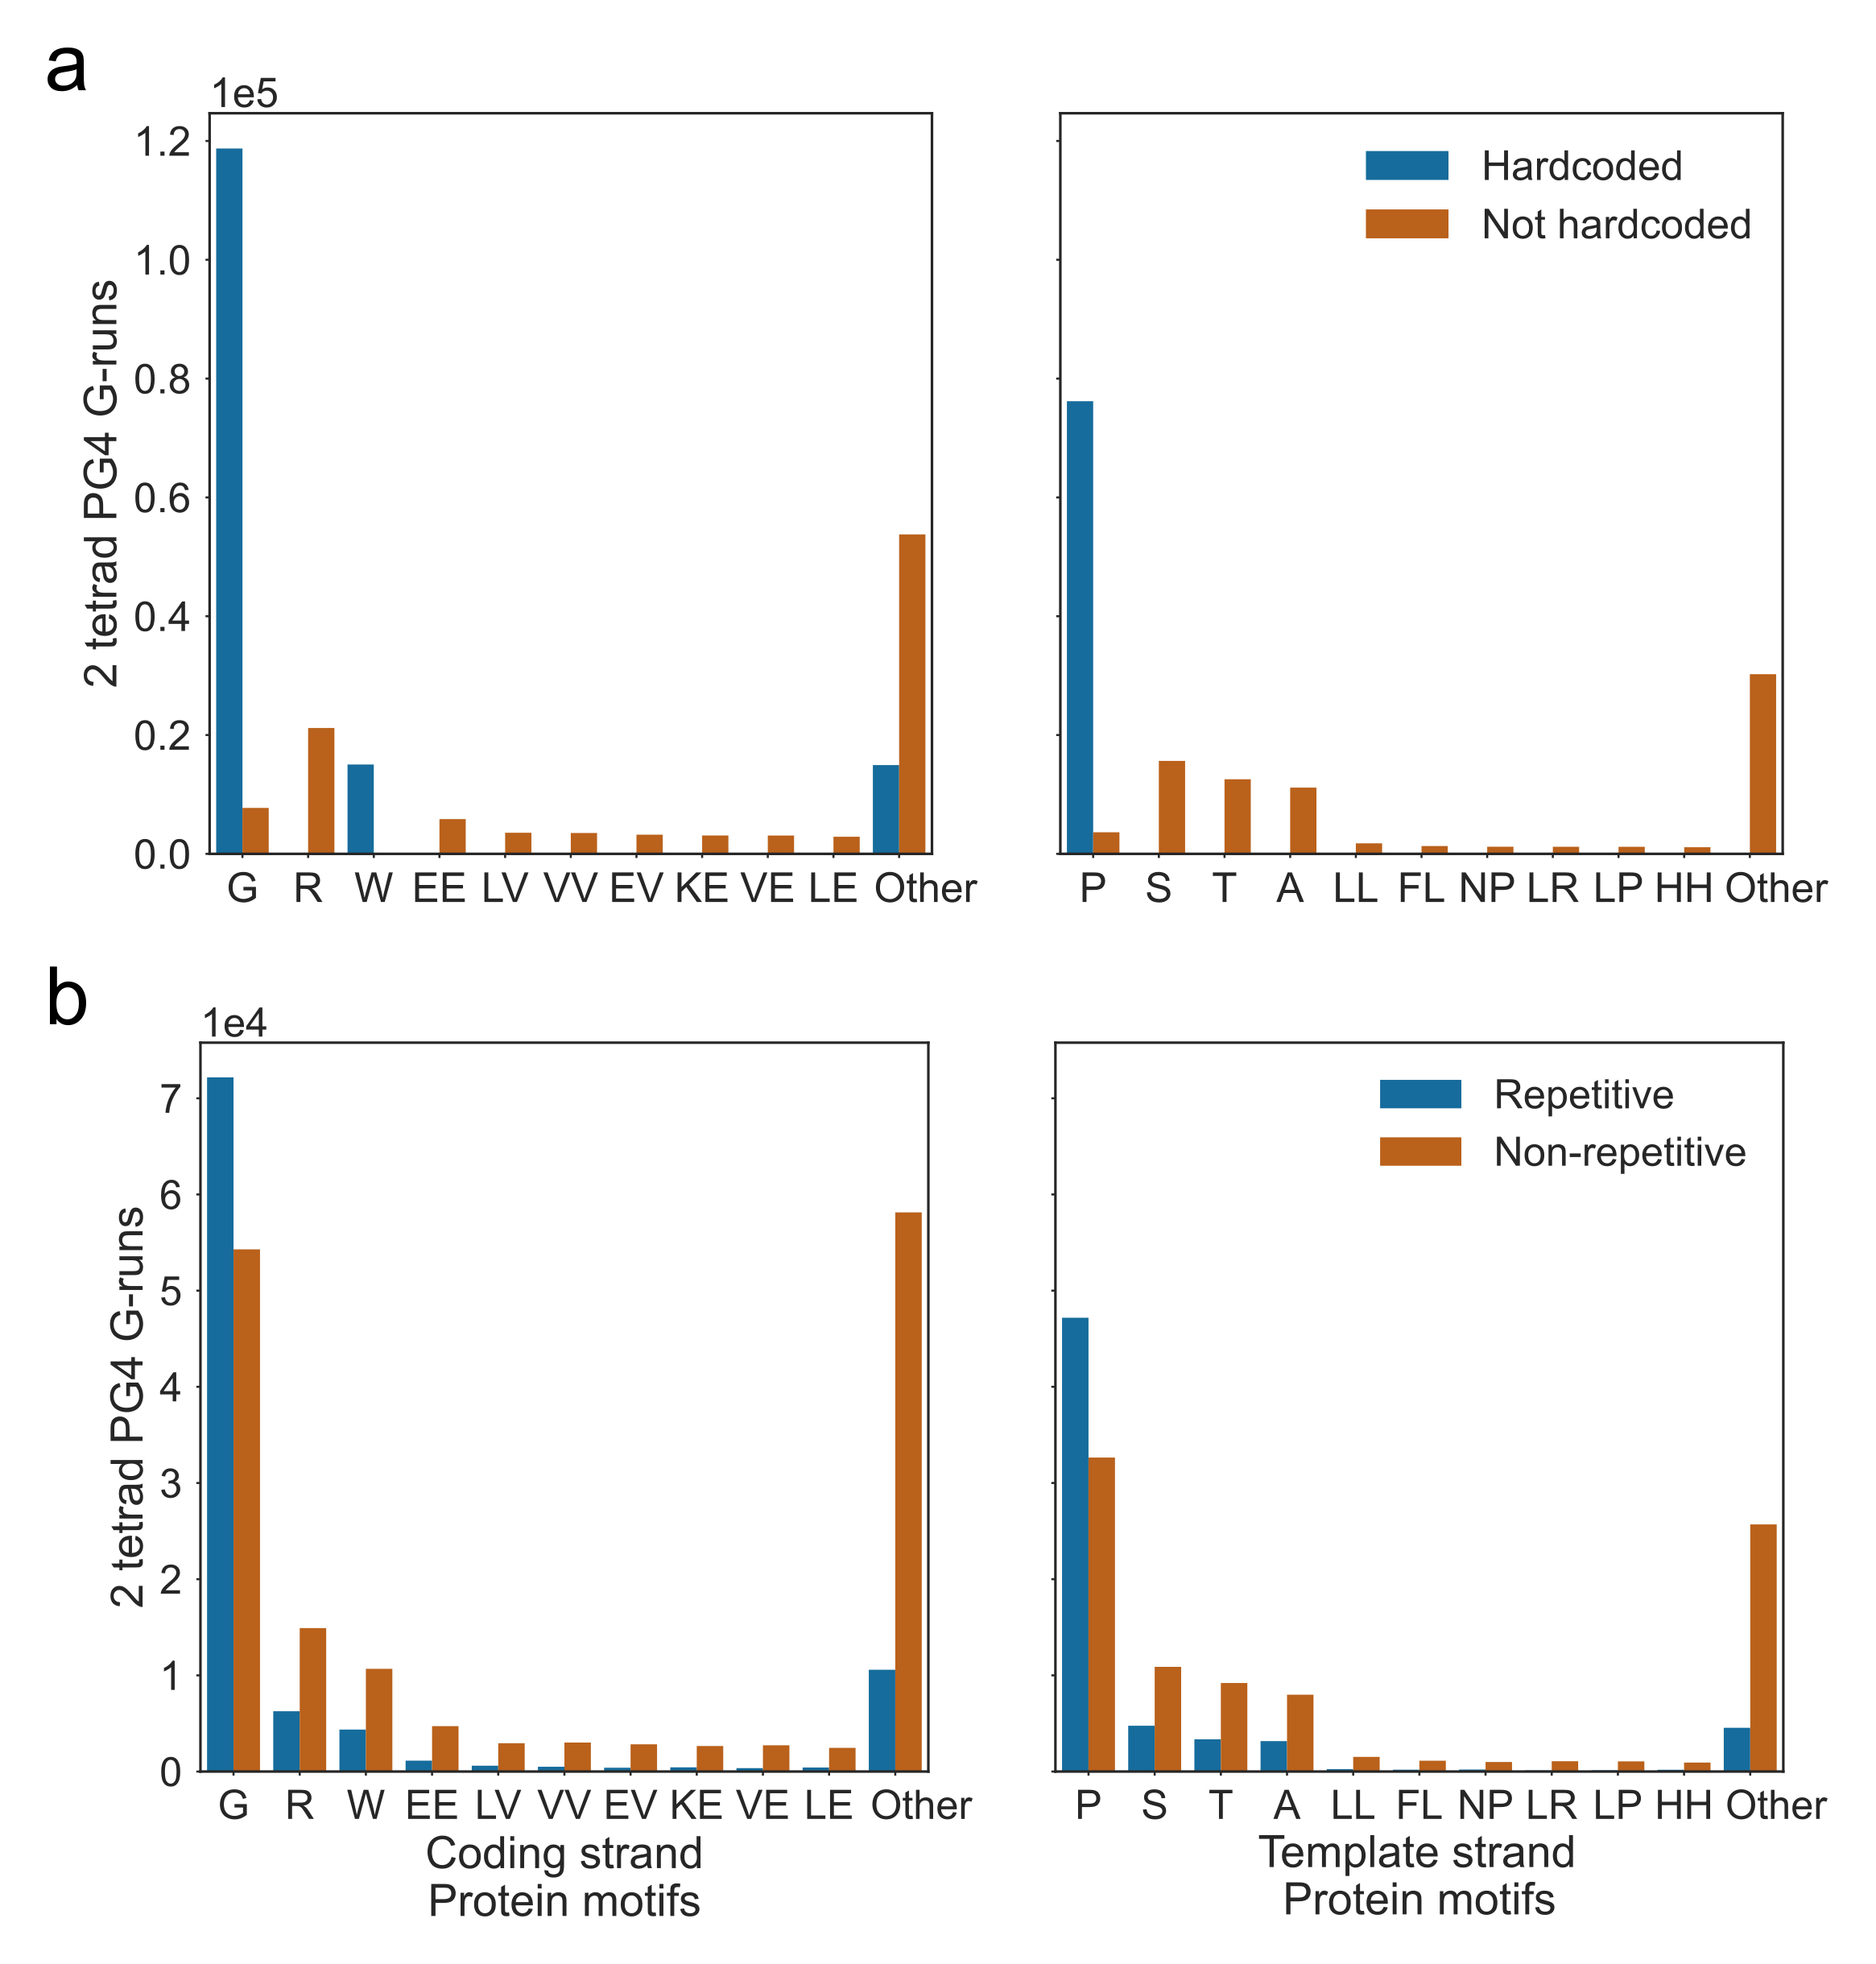
\includegraphics[width=\textwidth,height=562pt,keepaspectratio]{chapter_4/figures/pg4_protein_motifs.png}
\caption[Protein motifs that are coded by PG4 G-runs.]{\textbf{Protein   motifs   that   are   coded   by   PG4   G-runs.}   Frequency   plots   showing   the   10   most   common   amino   acids   motifs   which   PG4   G-runs   contribute   to   the   coding   of.   Left   and   right   panels   are   for   coding   and   template   strands,   respectively.   Bars   are   coloured   by   the   frequency   of   \textbf{a)}   hardcoded   and   \textbf{b)}   repetitive   G-runs,   respectively.   \label{protmotif}}
\end{figure}

\newpage

\hypertarget{discussion}{%
\section{Discussion}\label{discussion}}

The majority of analysis on the effects of G4s on biological processes
has thus far been conducted in mammalian systems, particularly in human
cells. The genomes of the mammals \emph{M. musculus} and \emph{H.
sapiens} are extremely rich in three tetrad PG4s compared to those of
most plants. Many plant genomes, particularly those of Monocots, have
comparable levels of two tetrad PG4s to the mammalian genomes, however.
Furthermore, the ratio of two tetrad to three tetrad PG4s in plant
genomes is much greater than in humans or mice, suggesting that in plant
systems, two tetrad PG4s may play a greater role in regulation that in
mammals. This is intuitive because plants tend to exist at more ambient
temperatures than warm-blooded mammals, and therefore the lower melting
temperatures of two tetrad PG4s might make them more favourable choices
for molecular switches than three tetrad PG4s.

The dicotyledon \emph{Arabidopsis thaliana} has a low three tetrad PG4
density but a relatively high two tetrad PG4 density. Previous analyses
by Mullen et al.~have identified that the majority of Arabidopsis two
tetrad PG4s are located inside genic regions, whilst the majority of
three tetrad PG4s are located in intergenic regions (Mullen et al.,
2010). We performed metagene profile analyses and showed that the levels
of two tetrad PG4s are greatest inside CDS regions on both the coding
and template strand. These levels were greatest at the start codon
proximal end on the template strand, and the distal end on the coding
strand. We also identified a peak of PG4s on the template strand in the
5' UTR. These levels are higher than would be expected from random
sequence with the same mononucleotide and dinucleotide frequencies,
suggesting that the sequence is ordered specifically to allow G4
formation. Since the template strand is scanned by RNA polymerase II
(Pol II) using transcription, it is possible that G4s which form in this
strand may cause blockages that slow or stall the progress of Pol II
using transcription. Since the levels of PG4s are greatest at the TSS
proximal end on this strand, these might perhaps be involved in proximal
pausing or slowing elongation initially to ensure modifications and
co-factors of the transcriptional complex are correct. Proximal pausing
is a common checkpoint of transcription in mammalian systems, but was
not identified by Hetzel et al.~in Arabidopsis or maize GRO-seq data
(Hetzel et al., 2016). Another possibility is that TSS proximal template
strand G4s might act as molecular switches which could cause premature
termination when folded, thereby regulating the expression of genes.

Since PG4 forming sequences in CDS regions must also code for protein
sequence, we were interested in identifying the degree to which PG4s are
determined by coding sequence. Some PG4 motifs cannot be removed from
the CDS without changing the protein sequence. We refer to these as
hardcoded PG4s. To explore this idea, we developed the reverse
translation simulation, where codon usage across the whole genome was
used to simulate potential coding sequences (PCSs) for each CDS, and the
number of PG4s in the real CDS vs the average PCS was compared. This
method identified that the G-content skew on both strands is heightened
by codon choice, however some G-content skew is also hardcoded by
protein sequence. This suggests that protein sequence may in fact be
under selection to increase template strand G-content at the start of
the CDS. We also found that the levels of PG4s on the coding strand of
real CDSs were lower than was expected from PCSs, i.e.~codon usage
selectively removes non-hardcoded PG4s on the coding strand. This is
possibly to remove obstacles to the ribosome during translation, since
coding strand PG4s may also form in the mRNA, and RNA G4s are more
stable than DNA G4s. The levels of coding strand PG4s were greater at
the distal end of the CDS in both real CDSs and simulated PCSs,
suggesting a greater level of hardcoded PG4s occur towards the end of
CDSs.

Reverse translation identifies that the levels of template strand PG4s
are greater in real CDSs than expected from PCSs at the start codon
proximal end. This enrichment falls through the CDS, and the second half
of the template strand CDS is depleted in PG4s. This suggests that PG4s
serve some purpose at the start of CDSs, perhaps in regulating Pol II
speed. Furthermore, we see a peak of template strand PG4s at the
proximal end of PCSs, suggesting that there are more hardcoded or
partially hardcoded PG4s at the proximal end, and that N-terminal
protein sequence may in fact be selected to allow PG4 formation in the
DNA.

To further explore the levels of hardcoded vs.~non-hardcoded PG4s in
Arabidopsis CDSs, we identified, for each overlapping PG4 register,
whether each G-run was hardcoded or not. The one or two amino acid motif
which was contributed to by each G-run was also determined. We found
that greater than 50\% of all PG4 G-runs are hardcoded, and 34\% of all
PG4s are totally hardcoded. The start codon proximal end of the template
strand contains the greatest number of non-hardcoded PG4s, explaining
the strong enrichment in this region compared to PCSs.

The most common amino acids which contribute to hardcoded PG4s are
glycine (codon GGN) on the coding strand, and proline (codon CCN) on the
template strand. G-runs encoding these amino acids also tend to be
repetitive, i.e.~contribute to PG4s in which all G-runs encode the same
amino acid motif. Poly-proline and poly-glycine rich motifs are common
in the Arabidopsis genome, and have some similar properties, including a
tendency to be intronless. Poly-glycine rich proteins (GRPs) are
involved in a number of processes, including cell elongation, plant
defense, and osmotic or salt stress (Mangeon et al., 2010). A number of
RNA-binding GRPs which have RNA chaperone activity are regulated by
osmotic stresses and by abscisic acid (Mangeon et al., 2010).
Interestingly, the cellular concentration of G4 stabilising potassium
cations is increased during these stresses, suggesting that G4s may be
more favourable. Mullen et al.~have previously suggested that
intracellular potassium concentrations might regulate two tetrad G4
formation in Arabidopsis mRNAs, causing conformational changes in the
RNA (Mullen et al., 2012). Furthermore, Kim et al.~used SELEX to
identify that the stress responsive RNA chaperone GRP7 binds
preferentially to G-rich single stranded DNA or RNA (Kim et al., 2006),
though they did not test whether these formed G4s. It is possible that
GRPs are involved in a feedback mechanism, stabilising mRNAs (including
their own mRNAs) during stress by either binding to or resolving G4s in
the mRNA.

Poly-proline rich proteins are often structural proteins, and are a
major constituent of the plant cell wall. Proline rich motifs form PG4s
in the template strand of DNA. These will not form in the mRNA, but may
cause issues for Pol II using transcription. This will be discussed
further in \ref{chap:global_nmm} and \ref{chap:extensins}.

\newpage

\hypertarget{global-effect-of-g-quadruplex-stabilisation-on-gene-expression}{%
\chapter{Global effect of G Quadruplex stabilisation on gene
expression}\label{global-effect-of-g-quadruplex-stabilisation-on-gene-expression}}

\label{chap:global_nmm}

\hypertarget{introduction-3}{%
\section{Introduction}\label{introduction-3}}

As was shown in Chapter 4, the distribution of PG4s around and within
genic regions is not uniform. In the \emph{Arabidopsis thaliana} genome,
template stranded PG4s are enriched in the 5' UTRs and promoter proximal
regions, whilst coding strand PG4s are enriched in 3' UTRs and promoter
distal regions. These enrichments do not appear to be explained simply
by the GC content of these sequences, nor by the requirement to code for
particular amino acids. These features may be deliberately conserved,
indicating a biological function for PG4s within gene bodies. As G4s are
formed from single stranded DNA, it has been previously hypothesised
that coding strand G4s might function to promote transcription by
competing with double stranded DNA to produce regions of open chromatin
which could easily become transcription bubbles (Rhodes and Lipps,
2015). G4s in the coding strand also have an opportunity to form in mRNA
and regulate stability, splicing or translation. Template stranded G4s
which occur downstream of translocating RNA Polymerase II (Pol II), on
the other hand, might cause blockages which prevent elongation, causing
downregulation of the gene (Rhodes and Lipps, 2015).

Arguably the best \emph{in vivo} evidence for G4 formation was conducted
using an antibody raised against G4 structures, referred to as BG4. BG4
was used to visualise G4s in human cancer cells by immunofluorescence
(Biffi et al., 2013). G4 foci were identified at both the telomeres
(which are highly GC rich and have been shown to form G4s \emph{in
vitro}), and in interstitial regions which contain actively transcribed
euchromatin. The G4 density of the cells was also seen to fluctuate
throughout the cell cycle, with the greatest number of foci appearing
during S phase, when the DNA is decondensed to allow replication to
occur.

The BG4 antibody has been further used to conduct ChIPseq experiments in
human cell lines, in which the DNA fragments to which the antibody binds
were enriched and subsequently sequenced (Hänsel-Hertsch et al., 2016).
BG4 ChIPseq peaks were found to overlap with regions of open chromatin
which are sensitive to DNAse digestion. These regions are commonly found
around the transcriptional start sites of genes and are associated with
actively transcription or promoter proximal pausing. Interestingly,
genes in which BG4 peaks strengthened after treatment with HDAC
inhibitors (which cause relaxation of heterochromatin) also saw a
corresponding increase in gene expression, suggesting that promoter G4
formation may have a positive impact upon gene expression
(Hänsel-Hertsch et al., 2016).

Another method by which the effect of G4s on transcription has been
studied is through stabilisation with G4 binding ligands. These ligands
generally bind to G4s through external hydrophobic pi-stacking above a
planar tetrad, or through intercalation between the inner faces of
tetrads. Treatment of yeast species \emph{Saccharomyces cerevisiae} with
the G4 stacking ligand N-methyl-mesoporphyrin was shown to upregulate
the expression of genes containing coding strand G4s in their promoters
(Hershman et al., 2008). Rodriguez et al.~showed that treatment of human
cells with Pyridostatin caused DNA damage at PG4 containing regions in
gene bodies, caused by both replication dependent and transcription
dependent damage (Rodriguez et al., 2012). These genes were also
downregulated in expression, suggesting that stabilised G4s caused
arrest of Pol II. G4s have also been shown to cause pausing of
polymerases \emph{in vitro}, in the presence and absence of G4 binding
ligands (Han et al., 1999; Siddiqui-Jain et al., 2002; Cogoi and Xodo,
2006; Dexheimer et al., 2006; Chambers et al., 2015; Kwok et al., 2016).

Here we conduct a global study of G4 stabilisation in the model plant
\emph{Arabidopsis thaliana}, using the G4 binding ligand NMM. Previous
studies have shown that treatment of Arabidopsis seedlings with NMM
cause developmental defects (Nakagawa et al., 2012), suggesting an
effect on gene expression. We also identify alterations in Pol II
occupancy potentially caused by G4 dense transcribed regions of genes.
Interestingly, Mullen et al.~showed that genes involved in response to
drought stress tended to be more likely to contain PG4s in their gene
bodies (Mullen et al., 2012). Since G4 formation is dependent upon
potassium cation concentration, the intracellular concentration of which
increases during drought stress, this could constitute a regulatory
mechanism of G4s. We also investigate the overlap of NMM regulated genes
with drought stress responsive genes.

\newpage

\hypertarget{methods}{%
\section{Methods}\label{methods}}

\hypertarget{plant-growth-conditions}{%
\subsection{Plant Growth Conditions}\label{plant-growth-conditions}}

For N-Methyl Mesoporphyrin (NMM) (Frontier Scientific, NMM580) treatment
microarray experiments, the \emph{Arabidopsis thaliana} Columbia (Col-0)
ecotype was used. Seeds were surface sterilised, stratified for 2-3 days
at 4°C and sown on vertical plates containing Murashige \& Skoog (MS)
agar with 0.5\% sucrose and 0.8\% agar. Plants were then transferred to
growth cabinets with 16 hours light at 23°C. Seedlings used for
expression analysis by qRT-PCR were grown for 7 days on MS plates,
treated for 6 hours by flooding the plate with MS liquid media
containing NMM after which roots and shoots are harvested separately.

\hypertarget{rna-extraction-microarray-data-generation}{%
\subsection{RNA Extraction \& Microarray data
generation}\label{rna-extraction-microarray-data-generation}}

Total nucleic acid isolation protocol was carried out by
phenol-chloroform extraction as described by White and Kaper (White and
Kaper, 1989). The resulting pellets were resuspended in sterile water
and stored at -80C. The RNA concentration and quality was checked using
the NanoDrop 1000 Spectrophotometer (ThermoScientific).

cDNA library preparation and microarray analysis were performed by the
Genomics Core Facility in the Sheffield Institute for Translational
Neuroscience. An Arabidopsis Gene 1.0 ST array was used. RNA integrity
and abundance was measured using an Aligent Bioanalyser 2100.
Hybridization and scanning procedures were conducted according to the
manufacturer using the Affymetrix Gene Chip hybridisation system.

\hypertarget{microarray-analysis}{%
\subsection{Microarray Analysis}\label{microarray-analysis}}

NMM Microarray analysis was conducted in R using the packages
\texttt{oligo} and \texttt{puma} (Pearson et al., 2009; Carvalho and
Irizarry, 2010; Liu et al., 2013). \texttt{oligo/puma} was chosen over
\texttt{oligo/limma} (Ritchie et al., 2015) for this analysis as NMM
treatment appeared to cause large consistent changes in gene expression
which violated the assumptions used in Robust Multi-chip Averaging
(RMA), namely that most genes do not change there expression and that
there is no correlation between average expression and log fold change.
CEL files were read into R using \texttt{oligo} but were not normalised
using RMA. The \texttt{puma} Bayesian probabilistic method was used to
normalise data and conduct differential expression analysis.
\texttt{puma} Probability of Positive Log Ratio (PPLR) values were
calculated for each contrast. Strongly differentially expressed genes
were produced using an absolute log2 fold change threshold of 1 and a
PPLR of 0.05 (or 0.95 for positively differentially expressed genes),
and moderately differentially expressed genes were produced using an
absolute log2 fold change threshold of 0.5 and a PPLR of 0.05.
Annotation of microarray data was conducted using the
\texttt{oligo\ getNetAffx} function and Ensembl annotations were
extracted.

\hypertarget{analysis-of-previously-published-microarray-data}{%
\subsection{Analysis of previously published microarray
data}\label{analysis-of-previously-published-microarray-data}}

Processed Berberine expression data was downloaded from the
supplementary material of Nakagawa et al.~2012. Data was generated using
an Affymetrix ATH1 GeneChip array from Col-0 plants grown on MS media
containing 12.5μM Berberine for 14 days.

Drought stress microarrays were downloaded from GSE65414 (Linster et
al., 2015). Drought stressed plants were grown on soil for 6 weeks under
with 8 hour light period, with normal watering, followed by 10 days
drought stress. Data was generated using the Affymetrix Gene 1.1 ST
Array.

Raw drought stress microarray data was processed in R using
\texttt{oligo} and \texttt{limma} (Carvalho and Irizarry, 2010; Ritchie
et al., 2015). CEL files were read into R using \texttt{oligo} and
quantile normalised \& median polished using Robust Multi-chip
averaging. Linear modelling was then performed using \texttt{limma}, and
p values were adjusted for multiple testing using Benjamini Hochberg
correction. Strongly differentially expressed genes were produced using
an absolute log2 fold change threshold of 1 and a FDR of 0.05, and
moderately differentially expressed genes were produced using an
absolute log2 fold change threshold of 0.5 and a FDR of 0.05. Annotation
of microarray data was conducted using the \texttt{oligo}
\texttt{getNetAffx} function and Ensembl annotations were extracted.

\hypertarget{genome-and-annotations-used}{%
\subsection{Genome and Annotations
used}\label{genome-and-annotations-used}}

All analyses were performed using the TAIR10 genome (The Arabidopsis
Genome Initiative, 2000), downloaded in fasta format from
arabidopsis.org, and the Araport11 genome annotation (Cheng et al.,
2017), downloaded in GTF format from araport.org. Annotations were
filtered to obtain protein coding genes only using the CGAT
\texttt{gtf2gtf} script (Sims et al., 2014). To obtain sets of genic
features such as exons, introns, CDS and UTRs, CGAT \texttt{gtf2gtf} was
also used. Overlapping exons from different isoforms of the same gene
were flattened to produce non-overlapping exons, and bed files of exons,
CDS, 5' UTRs and 3' UTRs were generated from these flattened exons using
\texttt{awk}. Bed files of introns were created using CGAT
\texttt{gtf2gtf} to generate exon ``complementation''. Bed files of
whole gene bodies were generated using CGAT \texttt{gtf2gtf} to merge
all intervals into a single interval spanning the entire gene.

\hypertarget{pg4-prediction}{%
\subsection{PG4 prediction}\label{pg4-prediction}}

G Quadruplex predictions in the TAIR10 genome were carried out using an
in-house script (g4predict) which utilises the Quadparser method
(Huppert and Balasubramanian, 2005). Results were filtered using a
dynamic programming approach, commonly used in interval scheduling, to
produce the greatest number of non-overlapping PG4s. Scripts can be
found on GitHub at https://github.com/mparker2/g4predict. To count G4s
per gene, the bed files containing PG4s were overlapped with bed files
generated from Araport11 for exon, intron, CDS, 5' UTR, 3' UTR and full
gene bodies. This was done using \texttt{bedtools\ intersect} in count
mode (Quinlan and Hall, 2010). PG4s on the template and coding strands
of gene features were counted separately. For multi-exon genes, counts
for different exons were summed using \texttt{awk} scripts, and counts
were normalised by length to get PG4 densities per kb. Barplots of
average PG4 density for various gene features and gene sets were
produced in python using \texttt{pandas} and \texttt{seaborn} (Mckinney,
2011; Waskom et al., 2014). Errorbars for these plots are estimated 68\%
confidence intervals generated using 1000 bootstrapped samples.
Statistical hypothesis testing was done using the Mann-Whitney U test.

Maximal PG4 densities were calculated using a sliding window of 200bp
generated using \texttt{bedtools\ makewindows}, with a step size of 5bp
(Quinlan and Hall, 2010). \texttt{bedtools\ map} was used to count the
number of PG4s overlapping each window. The score of the maximum scoring
200bp window overlapping the transcribed body (exons and introns) of a
gene was assigned as the maximal PG4 density of the gene, using
\texttt{bedtools\ map}. Coding and template strand densities were
calculated separately. Pointplots of average expression change during
NMM treatment for genesets with different maximal PG4 densities were
produced in python using \texttt{pandas} and \texttt{seaborn} (Mckinney,
2011; Waskom et al., 2014). Errorbars for these plots are estimated 68\%
confidence intervals generated using 1000 bootstrapped samples.
Statistical hypothesis testing was done using the Mann-Whitney U test.

For analyses where G4seeqer was used, PG4 predictions were conducted on
the TAIR10 genome using the G4seeqer command line tool. A step size of
5bp and G4Hunter threshold of 0.75 were used. All intervals tested using
G4seeqer were output regardless of neural network score (i.e.~a
threshold of 0 was used). Maximum G4seeqer score overlapping each gene
body (exons and introns) was calculated using \texttt{bedtools\ map}
(Quinlan and Hall, 2010). Coding and template strand scores were
calculated separately.

\hypertarget{self-organising-map-analysis}{%
\subsection{Self Organising Map
Analysis}\label{self-organising-map-analysis}}

Loop lengths and total loop lengths for each Quadparser 2 tetrad PG4 in
the TAIR10 genome were extracted from bed files output by g4predict.
PG4s which did not overlap with gene bodies were discarded. Self
Organising Maps were trained in R using the package \texttt{kohonen} on
loop length data (Wehrens and Buydens, 2007). 36 clusters were used. To
identify enrichment of specific clusters of PG4s in NMM downregulated
genes, the total number of PG4s from each cluster overlapping the
geneset was calculated, and compared to an expected number of overlaps
computed by permuting PG4s amongst all genes. Genes were weighted by
length such that a 2kb gene was twice as likely to be assigned PG4s as a
1kb gene. Coding and template strand PG4s were permuted separately. The
log fold change between observed and expected overlap was then
calculated for each cluster. SOM plots were made in Python using
\texttt{matplotlib} (Hunter, 2007).

\hypertarget{venn-diagrams}{%
\subsection{Venn diagrams}\label{venn-diagrams}}

Venn diagrams of geneset overlaps were produced in Python using the
package \texttt{matplotlib\_venn}. Statistical hypothesis testing of
overlaps was conducted using hypergeometric tests.

\hypertarget{pol-ii-chip-tiling-array-analysis}{%
\subsection{Pol II ChIP-tiling array
analysis}\label{pol-ii-chip-tiling-array-analysis}}

RNA Polymerase II ChIP-tiling array data was downloaded from GEO
Accession GSE21673 (Chodavarapu et al., 2010). Plants were grown under
24hr light on soil for 10-14 days before being harvested. ChIP was
conducted using Abcam ab817 Pol II antibody and tiling arrays used were
Affymetrix Arabidopsis Tiling 1.0R Array. Pol II occupancy tracks were
generated from CEL files in R using \texttt{STARR} (Zacher et al.,
2010). Cyclic lowess method was used for probe intensity normalisation.
The enrichment ratio of PolII signal intensity over control was
calculated and saved in BigWig format using \texttt{rtracklayer}
(Lawrence et al., 2009). Metagene profiles for all genes were produced
using CGAT \texttt{bam2geneprofile} (Sims et al., 2014). Gene profiles
of merged exons (without introns) were produced using 100 bins across
the gene body, with an upstream and downstream extension of 500bp at
10bp resolution (i.e.~binned in 10bp intervals).

To compared Pol II occupancy of G4 containing genes with non-G4
containing genes, genesets with max G4seeqer scores greater than 0.95
and less than 0.05, or maximal PG4 density greater than 2 or equal to
zero were used. Metagene profile matrices were read into Python using
\texttt{pandas} and averaged profiles for each geneset were generated
using \texttt{seaborn} bootstrapping to estimate central tendency and
confidence intervals (Mckinney, 2011; Waskom et al., 2014). Bootstrapped
profiles were smoothed using a moving average of 20. 1000 iterations
were used for all bootstraps. Profiles were normalised so that the
absolute area under the curve was equal to one.

\hypertarget{grorna-seq-analysis}{%
\subsection{GRO/RNA seq analysis}\label{grorna-seq-analysis}}

Global Run On (GRO) and RNA sequencing data from GEO Accession GSE83108
(Hetzel et al., 2016) was downloaded from the European Nucleotide
Archive (ENA). Quality control analyses were performed using
\texttt{FastQC} and \texttt{fastq-screen} (Andrews, 2010; Wingett,
2011). Mapping to the TAIR10 genome with splice junction annotations
from Araport11 (The Arabidopsis Genome Initiative, 2000; Cheng et al.,
2017) was conducted using \texttt{STAR} (Dobin et al., 2013) with
default parameters, and generated BAM files were sorted using
\texttt{samtools} (Li et al., 2009). Exonic read counts per gene were
then counted using \texttt{featureCounts}(Liao et al., 2013). Read
counts were normalised for library depth in R (R Core Team, 2013) using
\texttt{DESeq2} (Love et al., 2014) and log2 transformed to get log
counts per million (logCPM). The ratio of GROseq to RNAseq reads was
calculated by subtracting the average RNAseq logCPM from the average
GROseq logCPM. Scatter plots of RNAseq logCPM vs GROseq logCPM were
generated in Python using \texttt{seaborn} (Waskom et al., 2014).

To contrast GRO/RNA seq ratios of G4 containing genes with non-G4
containing genes, genesets with max G4seeqer scores greater than 0.95
and less than 0.05, or maximal PG4 density greater than 2 or equal to
zero were used. Overlayed histograms and kernel density estimate plots
of GRO/RNA seq ratio for these genesets were generated using
\texttt{seaborn} (Waskom et al., 2014). Statistical hypothesis testing
was conducted using Welch's unpaired T-test.

\newpage

\hypertarget{results-1}{%
\section{Results}\label{results-1}}

\hypertarget{nmm-causes-global-change-in-gene-expression}{%
\subsubsection{NMM causes global change in gene
expression}\label{nmm-causes-global-change-in-gene-expression}}

In order to test the effect of G4 stabilisation on gene expression in
Arabidopsis, we conducted a microarray analysis using RNA from 7 day old
seedlings treated with NMM for 6 hours. Control samples were treated
with DMSO for 6 hours. We found 858 and 1098 genes were differentially
upregulated and downregulated respectively using a log fold change
threshold of 1 (PPLR \textless{} 0.05). When a less stringent log fold
change threshold of 0.5 was used (PPLR \textless{} 0.05), downregulated
genes outnumbered upregulated by a ratio of 2:1 (3882 downregulated,
1930 upregulated), suggesting that NMM has a global effect on gene
expression unlikely to be caused by a single transcription factor. An MA
plot of average gene expression vs log fold change, with lowess curve
fitting, showed that there appeared to be a slight skew towards
downregulation in genes with higher average expression (Fig \ref{nmm}a).
To more clearly visualise this skew we binned genes by average
expression quartile (Fig \ref{nmm}b). This showed there was indeed a
relationship between average expression and expression change upon NMM
treatment, with highly expressed genes tending to be more downregulated
by NMM treatment. This global pattern, which violates some of the
assumptions that are usually used in microarray normalisation and
analysis, suggests a widespread effect of NMM directly upon either
transcription or mRNA stability.

\newpage

\begin{figure}[htbp]
\centering
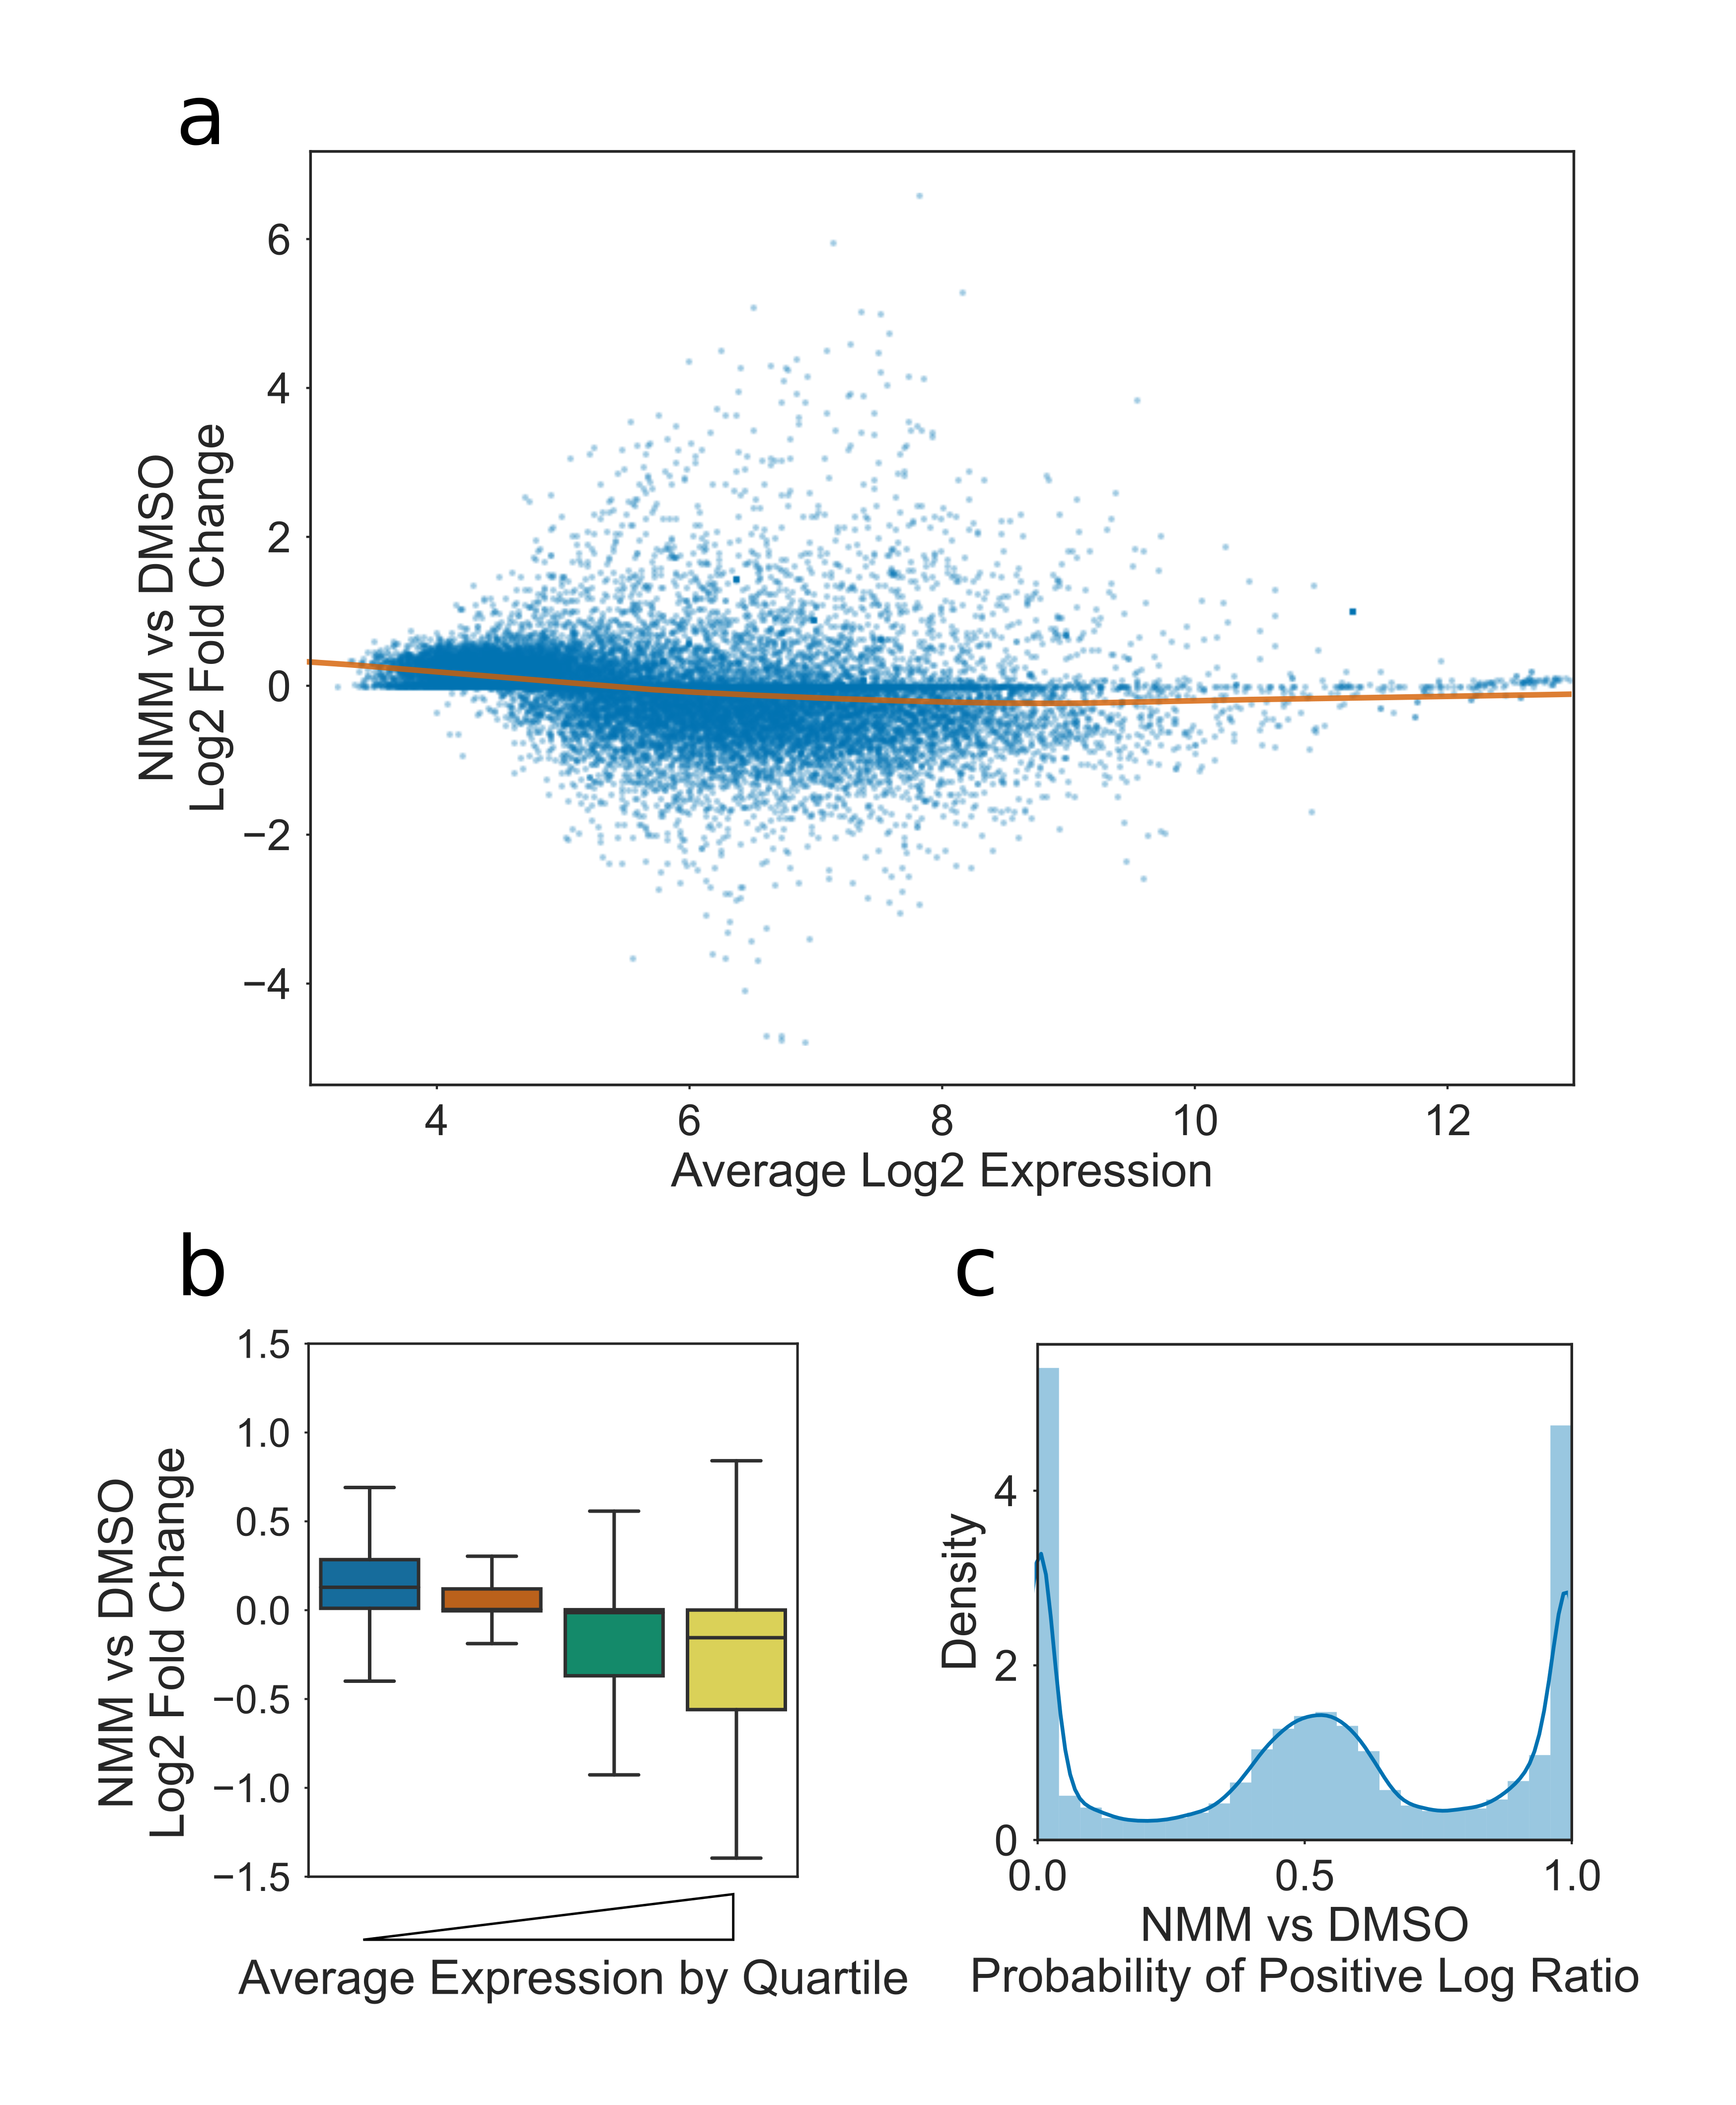
\includegraphics[width=\textwidth,height=562pt,keepaspectratio]{chapter_5/figures/nmm_vs_dmso.png}
\caption[Global effect of NMM on Gene Expression.]{\textbf{Global   effect   of   NMM   on   Gene   Expression.}   \textbf{a)}   MA   plot   showing   relationship   between   average   gene   expression   and   Log2   fold   change   in   expression   upon   treatment   with   NMM.   Orange   line   is   lowess   curve   fit   showing   slight   negative   correlation   between   expression   and   fold   change   for   genes   in   the   expression   range   4-8.   \textbf{b)}   Boxplot   of   Log2   fold   change   in   expression   upon   treatment   with   NMM,   cut   on   quartiles   by   average   expression.   Lowest   expressed   25\%   is   leftmost,   and   highest   expressed   is   rightmost.   Lower   quartile,   median,   and   upper   quartile   are   at   4.6,   5.4,   and   6.5,   respectively.   \textbf{c)}   Histogram   and   kernel   density   estimate   showing   distribution   of   Probability   of   Positive   Log   Ratio   (PPLR)   values.   PPLRs   which   tend   towards   zero   represent   negatively   differentially   expressed   genes,   whilst   PPLRs   which   tend   towards   one   represent   positively   differentially   expressed   genes.   \label{nmm}}
\end{figure}

\newpage

To support the hypothesis that NMM alters gene expression through G4
stabilisation, we correlated our results with processed data from a
Berberine treatment array (Fig \ref{berberine}a) (Nakagawa et al.,
2012). Berberine is another G4 stabilising drug, but with a very
different structure and method of action (intercalation with G4s rather
than hydrophobic stacking). Despite the differences in structure of the
two drugs, and the very different conditions (plants were grown on
Berberine for 14 days, compared with 6 hour treatment of 7 day old
seedlings with NMM), the log fold changes from our data correlated well
with the Berberine dataset (Pearsons R: 0.43, Spearman's ρ: 0.44). There
was a strong overlap between the genes downregulated by NMM and those
downregulated by Berberine (Fig \ref{berberine}b, p=1.1e-36). These
results suggest that the main effects on gene expression were through G4
interaction, with any off target effects being less significant
contributors.

\newpage

\begin{figure}[htbp]
\centering
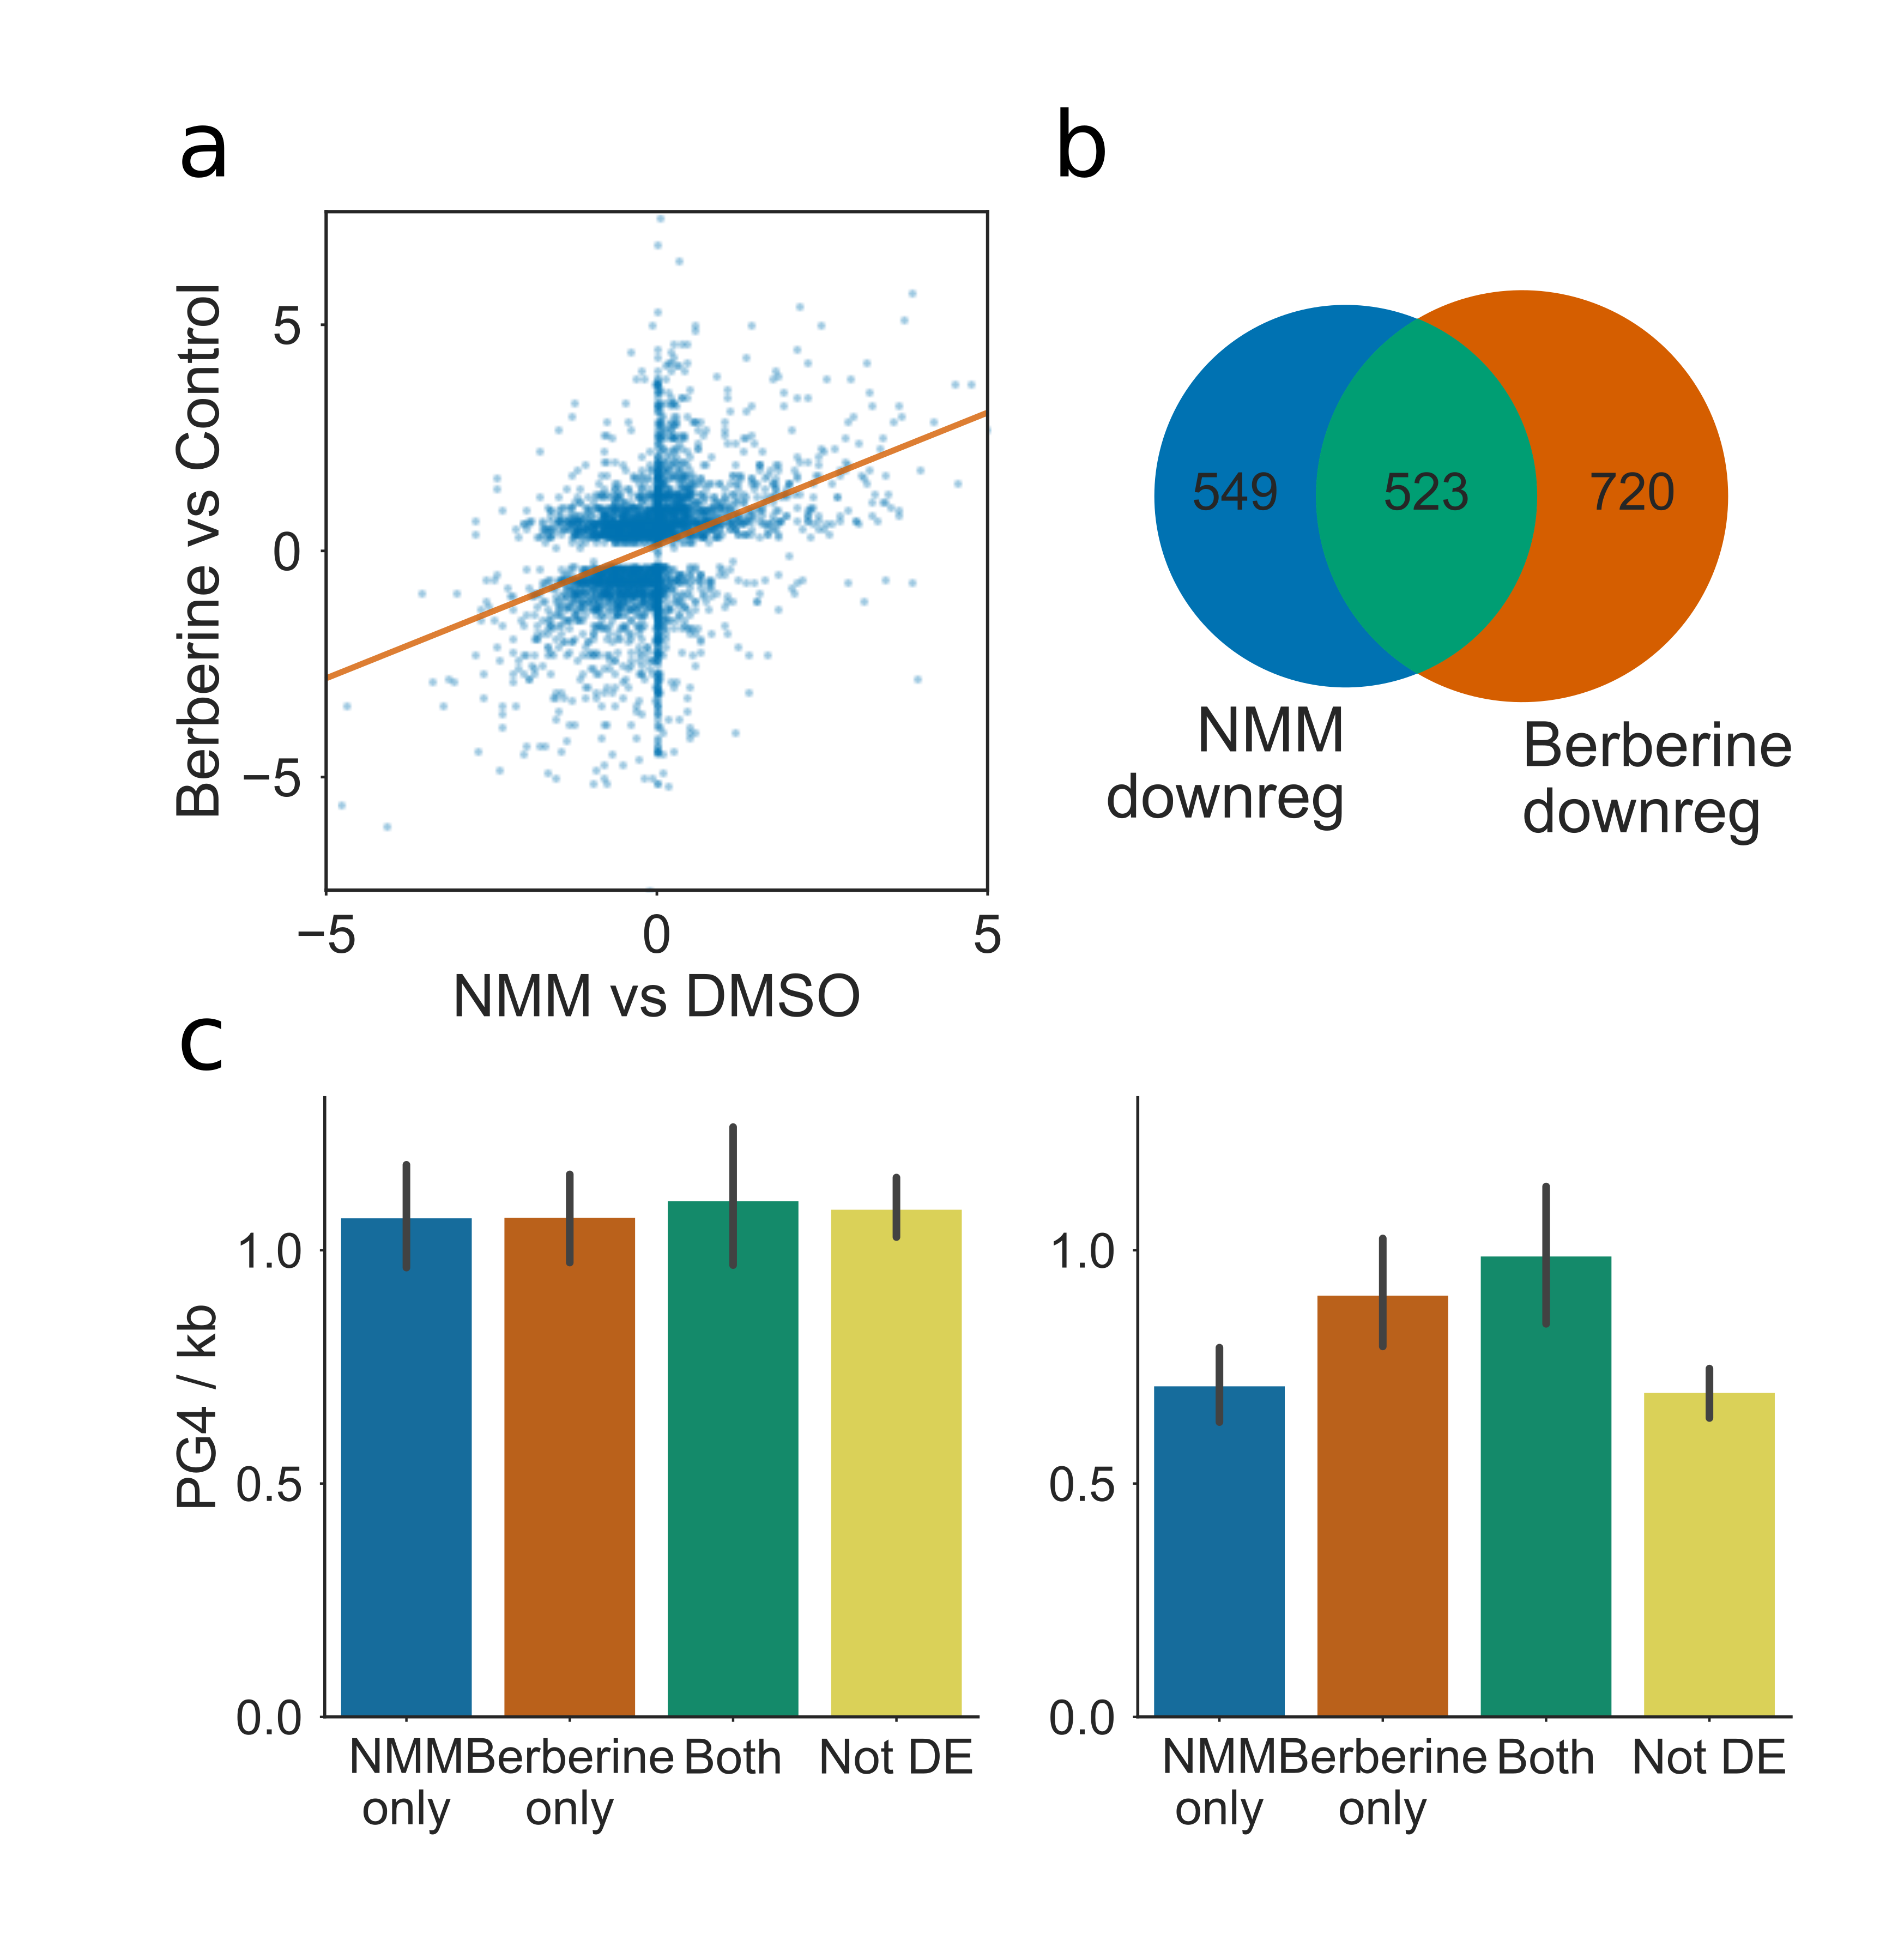
\includegraphics[width=\textwidth,height=562pt,keepaspectratio]{chapter_5/figures/nmm_berberine.png}
\caption[Comparison of gene expression during NMM treatment with expression during Berberine treatment.]{\textbf{Comparison   of   gene   expression   during   NMM   treatment   with   expression   during   Berberine   treatment.}   \textbf{a)}   Scatter   plot   with   regression   line   showing   the   correlation   in   expression   change   for   NMM   vs   DMSO   and   Berberine   vs   Control.   Processed   Berberine   data   was   taken   from   supplementary   information   of   Nakagawa   et   al. 2012,   however   only   differentially   regulated   genes   were   reported.   \textbf{b)}   Venn   diagram   reporting   the   overlap   of   genes   downregulated   by   NMM   with   those   downregulated   by   Berberine.   \textbf{c)}   Bar   plot   showing   the   average   exonic   PG4   densities   of   NMM   and   Berberine   downregulated   genesets,   on   the   coding   and   template   strands,   respectively.   Both   genesets   show   an   greater   exonic   G4   density   on   the   template   strand   than   genes   not   regulated   by   either   drug,   however   genes   which   are   regulated   by   both   drugs   had   the   greatest   average   exonic   PG4.   Bar   colours   match   set   colours   from   Fig   3b.   Errorbars   are   68\%   confidence   intervals   for   mean   generated   using   1000   bootstrapped   samples.   \label{berberine}}
\end{figure}

\newpage

\hypertarget{genes-downregulated-by-nmm-are-enriched-in-two-tetrad-pg4s}{%
\subsection{Genes downregulated by NMM are enriched in two tetrad
PG4s}\label{genes-downregulated-by-nmm-are-enriched-in-two-tetrad-pg4s}}

We next investigated whether NMM regulated genes were enriched for PG4s.
We first measured the density of PG4s in different regions of each gene
(i.e.~promoters, exons, introns, CDS and UTRs) and looked at the
differences between the differentially expressed gene sets at 6 hours
NMM treatment. We did not see a strong difference in three tetrad PG4
density in our gene sets, for any gene feature (data not shown). This is
likely due to the low density of these PG4s in Arabidopsis. We
discovered a striking enrichment of the 2 tetrad PG4s on the template
strand of genes which were down-regulated by NMM, with approximately
10\% more genes containing template PG4s than expected for a gene set of
that size (p=2e-48) (Fig \ref{nmm_g4_sq}). This enrichment occurred most
specifically in the CDS and 5' UTR regions of genes (Fig \ref{nmm_g4}).
Genes which were very strongly downregulated by NMM (logFC \textless{}
-1) tended to contain large numbers of PG4s throughout their exonic
bodies, particularly in coding regions and in the 5' UTR, whilst
moderately downregulated genes (logFC \textless{} -0.5) tended to have
greater concentration of PG4s in 5' UTRs.

\newpage

\begin{figure}[htbp]
\centering
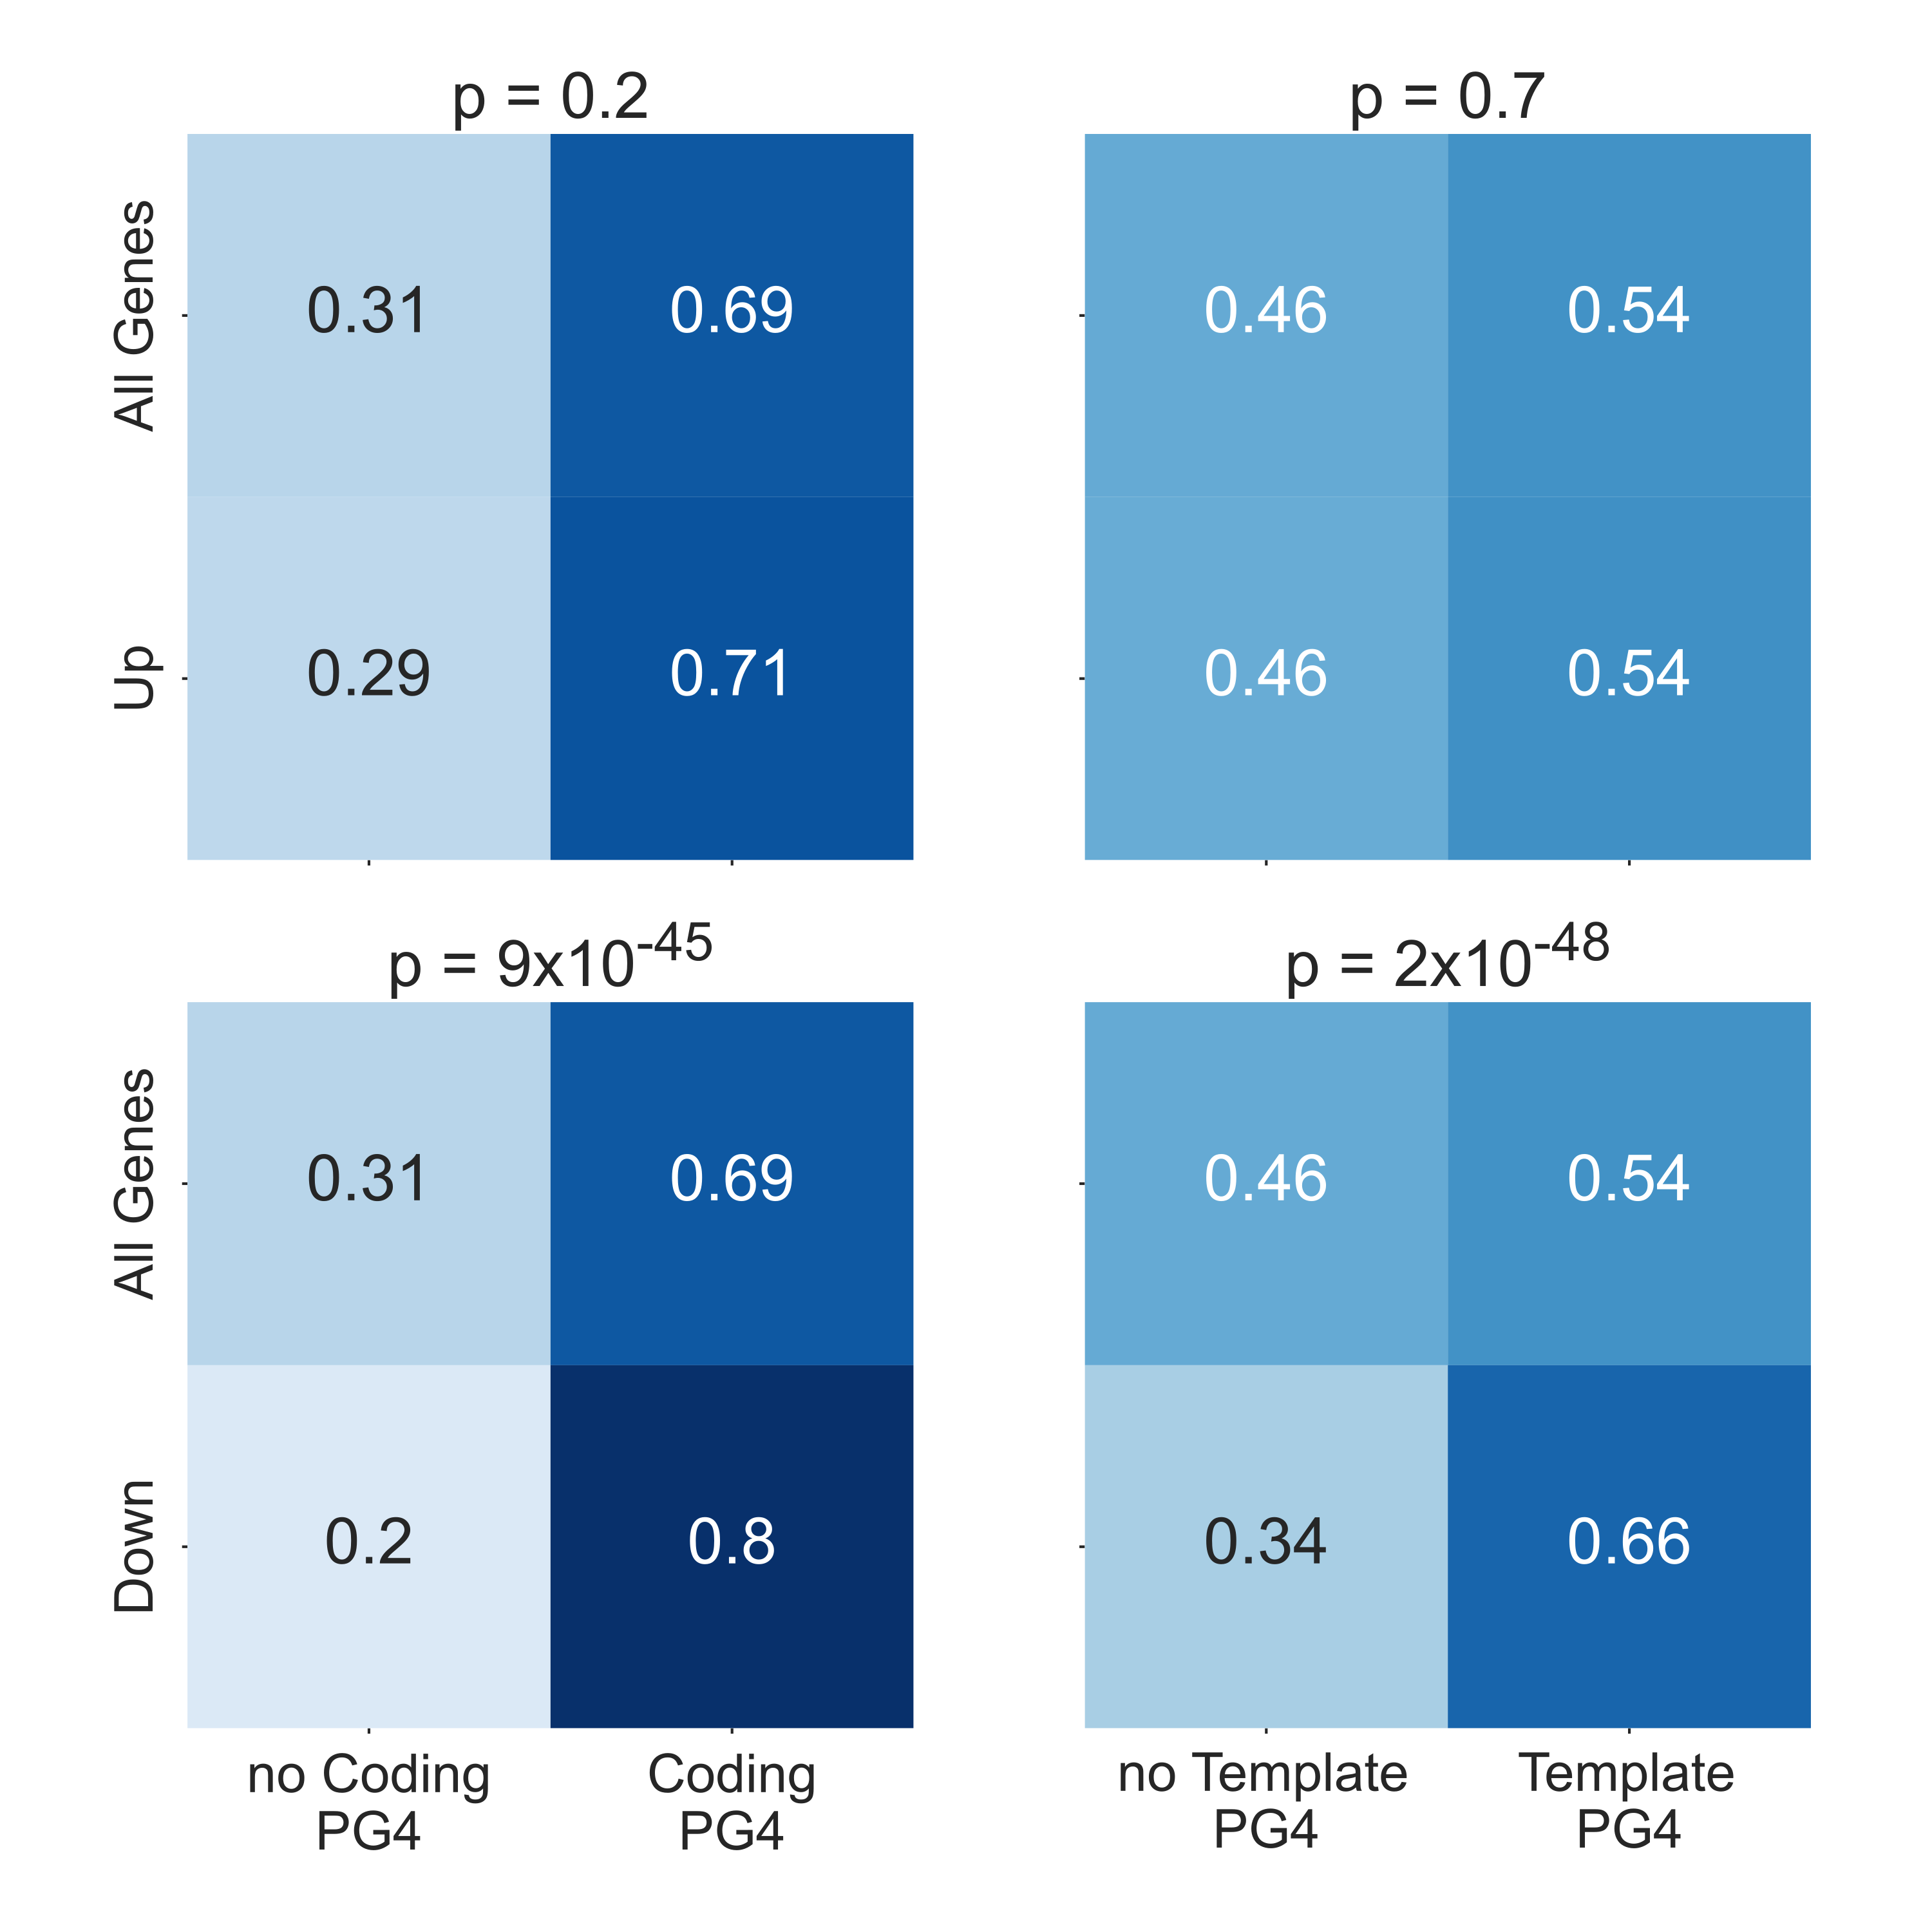
\includegraphics[width=\textwidth,height=562pt,keepaspectratio]{chapter_5/figures/nmm_g4_presence_absence_chisquared.png}
\caption[NMM downregulated genes are enriched in PG4s]{\textbf{NMM   downregulated   genes   are   enriched   in   PG4s}   Heatmaps   showing   fractions   of   genes   containing   at   least   one   predicted   G4   in   their   gene   body   for   upregulated   genes   vs   all   genes   (top   row)   and   downregulated   genes   vs   all   genes   (bottom   row)   (For   down   and   upregulated   genes,   FDR   <   0.05   and   absolute   logFC   >   0.5).   PG4   predictions   for   the   coding   strand   are   in   the   left   hand   column   whilst   PG4   predictions   for   template   strand   are   on   the   right.   P   values   for   each   heatmap   are   calculated   using   Chi-squared   tests.   Genes   downregulated   by   NMM   show   a   particularly   strong   enrichment   of   PG4s,   and   particularly   on   the   template   strand.   \label{nmm_g4_sq}}
\end{figure}

\newpage

\begin{figure}[htbp]
\centering
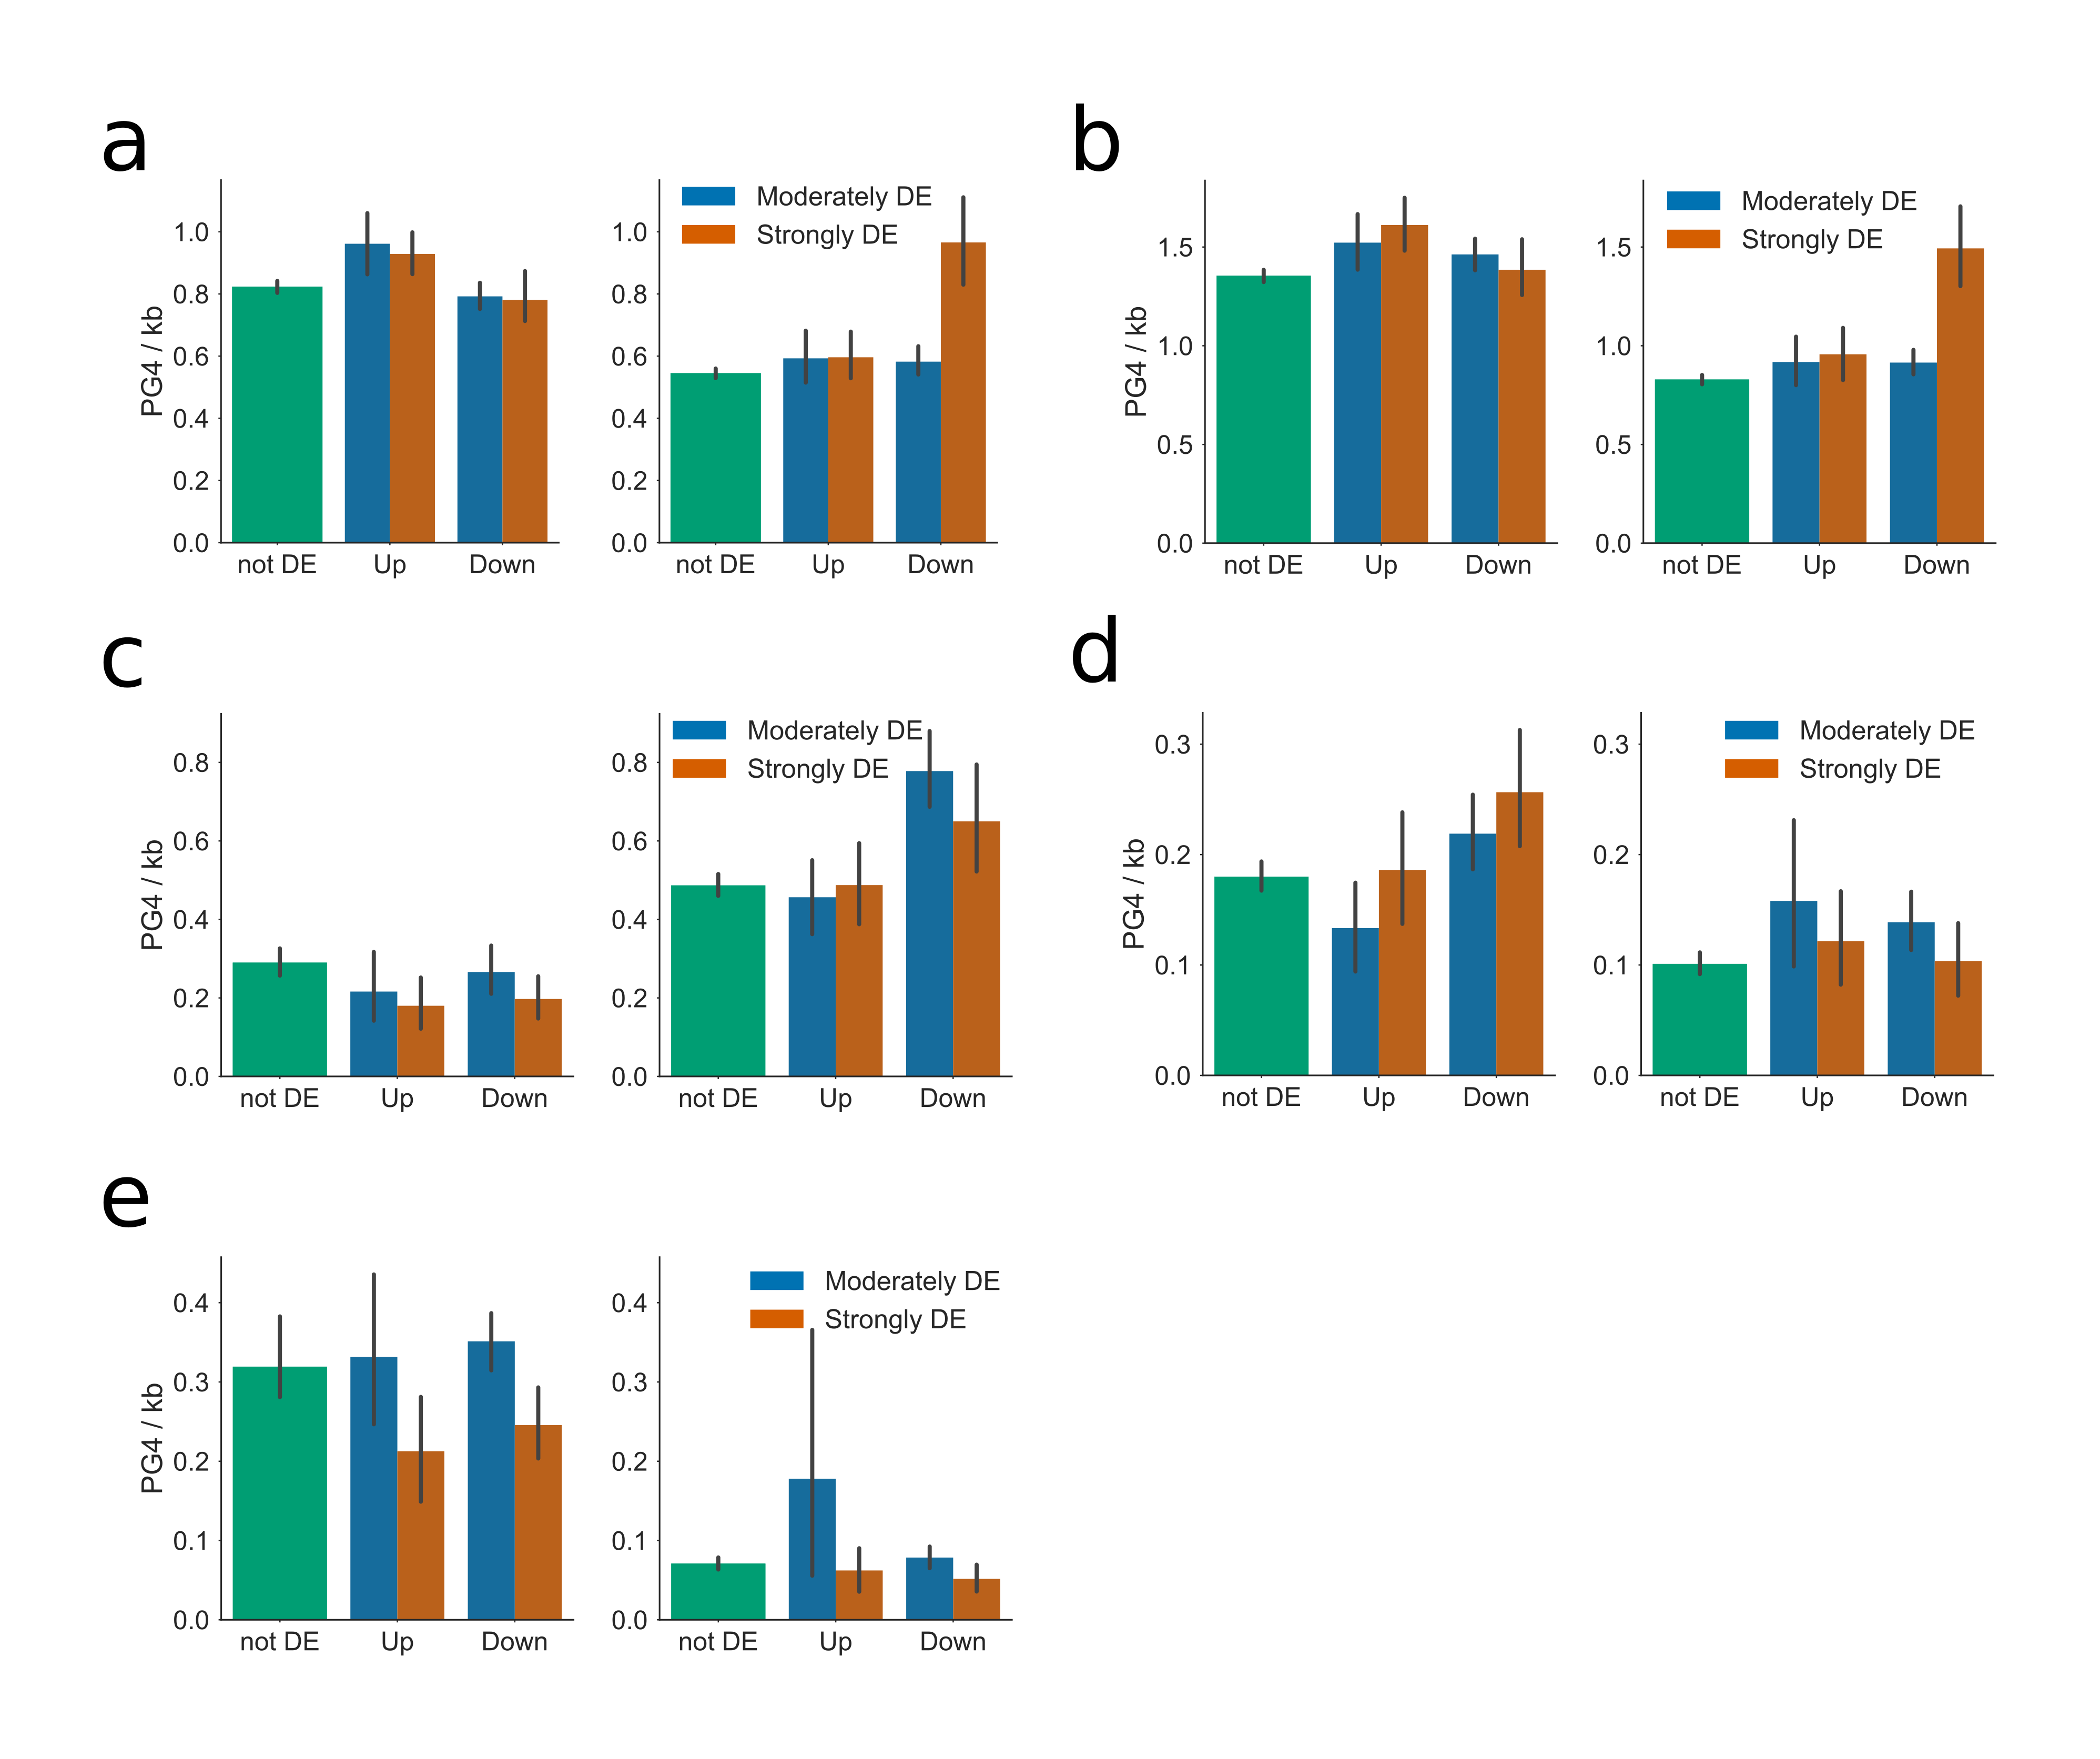
\includegraphics[width=\textwidth,height=562pt,keepaspectratio]{chapter_5/figures/nmm_regulated_g4_distribution.png}
\caption[Distribution of PG4s in genes differentially regulated by NMM.]{\textbf{Distribution   of   PG4s   in   genes   differentially   regulated   by   NMM.}   Bar   plots   showing   the   average   PG4   densities   of   genes   up   or   downregulated   by   NMM,   for   \textbf{a)}   full   gene   body   (exons   and   introns),   \textbf{b)}   coding   regions,   \textbf{c)}   5’   UTR,   \textbf{d)}   3’   UTR,   and   \textbf{e)}   introns,   respectively.   In   each   figure,   left   and   right   panels   represent   coding   and   template   strand,   respectively.   Genesets   are   separated   into   three   categories   by   strength   of   regulation:   green:   not   differentially   expressed,   blue:   moderately   differentially   expressed   (PPLR   <   0.05,   logFC   >   0.5),   orange:   strongly   differentially   expressed   (PPLR   <   0.05,   logFC   >   1).   Errorbars   are   68\%   confidence   intervals   for   mean   generated   using   1000   bootstrapped   samples.   Genes   which   are   strongly   downregulated   by   NMM   tend   to   have   higher   PG4   densities   on   the   template   strand   of   coding   regions   and   5’   UTRs,   whilst   moderately   downregulated   genes   tend   to   have   greater   PG4   density   on   the   template   strand   of   their   5’   UTRs.   \label{nmm_g4}}
\end{figure}

\newpage

The PG4 density of genes downregulated by both NMM and Berberine was
also calculated (Fig \ref{berberine}c). We found that whilst the gene
sets downregulated by either treatment were enriched in PG4s, those
which were in the intersection of the two sets had the greatest average
exonic PG4 density. This is further evidence that these drugs are
regulating gene expression through G4 stabilisation.

Previous studies have shown that NMM is highly selective towards
parallel G4s (Nicoludis et al., 2012b, 2012a; Tippana et al., 2014;
Kreig et al., 2015), and can induce anti-parallel G4s to switch
structure (Nicoludis et al., 2012b). G4s with short loop lengths are
more likely to form parallel structures (Tippana et al., 2014). In order
to test if NMM was selective towards G4s with particular loop lengths,
we used Self Organising Maps to cluster all predicted Arabidopsis 2
tetrad PG4s into 36 groups, based on the length of each loop 1-3, and
the total loop length (Fig \ref{som}b). Each cluster contained between
approximately 1000 and 8000 PG4s (Fig \ref{som}a). We then analysed the
relative enrichment of each PG4 cluster on each strand, within genes
which were downregulated by NMM, compared to permuted profiles across
all genes. No particular PG4 cluster was strongly enriched on the coding
strand of down-regulated genes (Fig \ref{som}c). One cluster, however,
was strongly enriched on the template strand (Fig \ref{som}d). This
cluster contained PG4s with very short loop lengths of 1-2bp and a total
loop length of 5-6bp. This conformed well with our prior expectations,
as G4s with short loop lengths are known to form propeller-like parallel
G4s of the kind favoured by NMM (Nicoludis et al., 2012b).

\newpage

\begin{figure}[htbp]
\centering
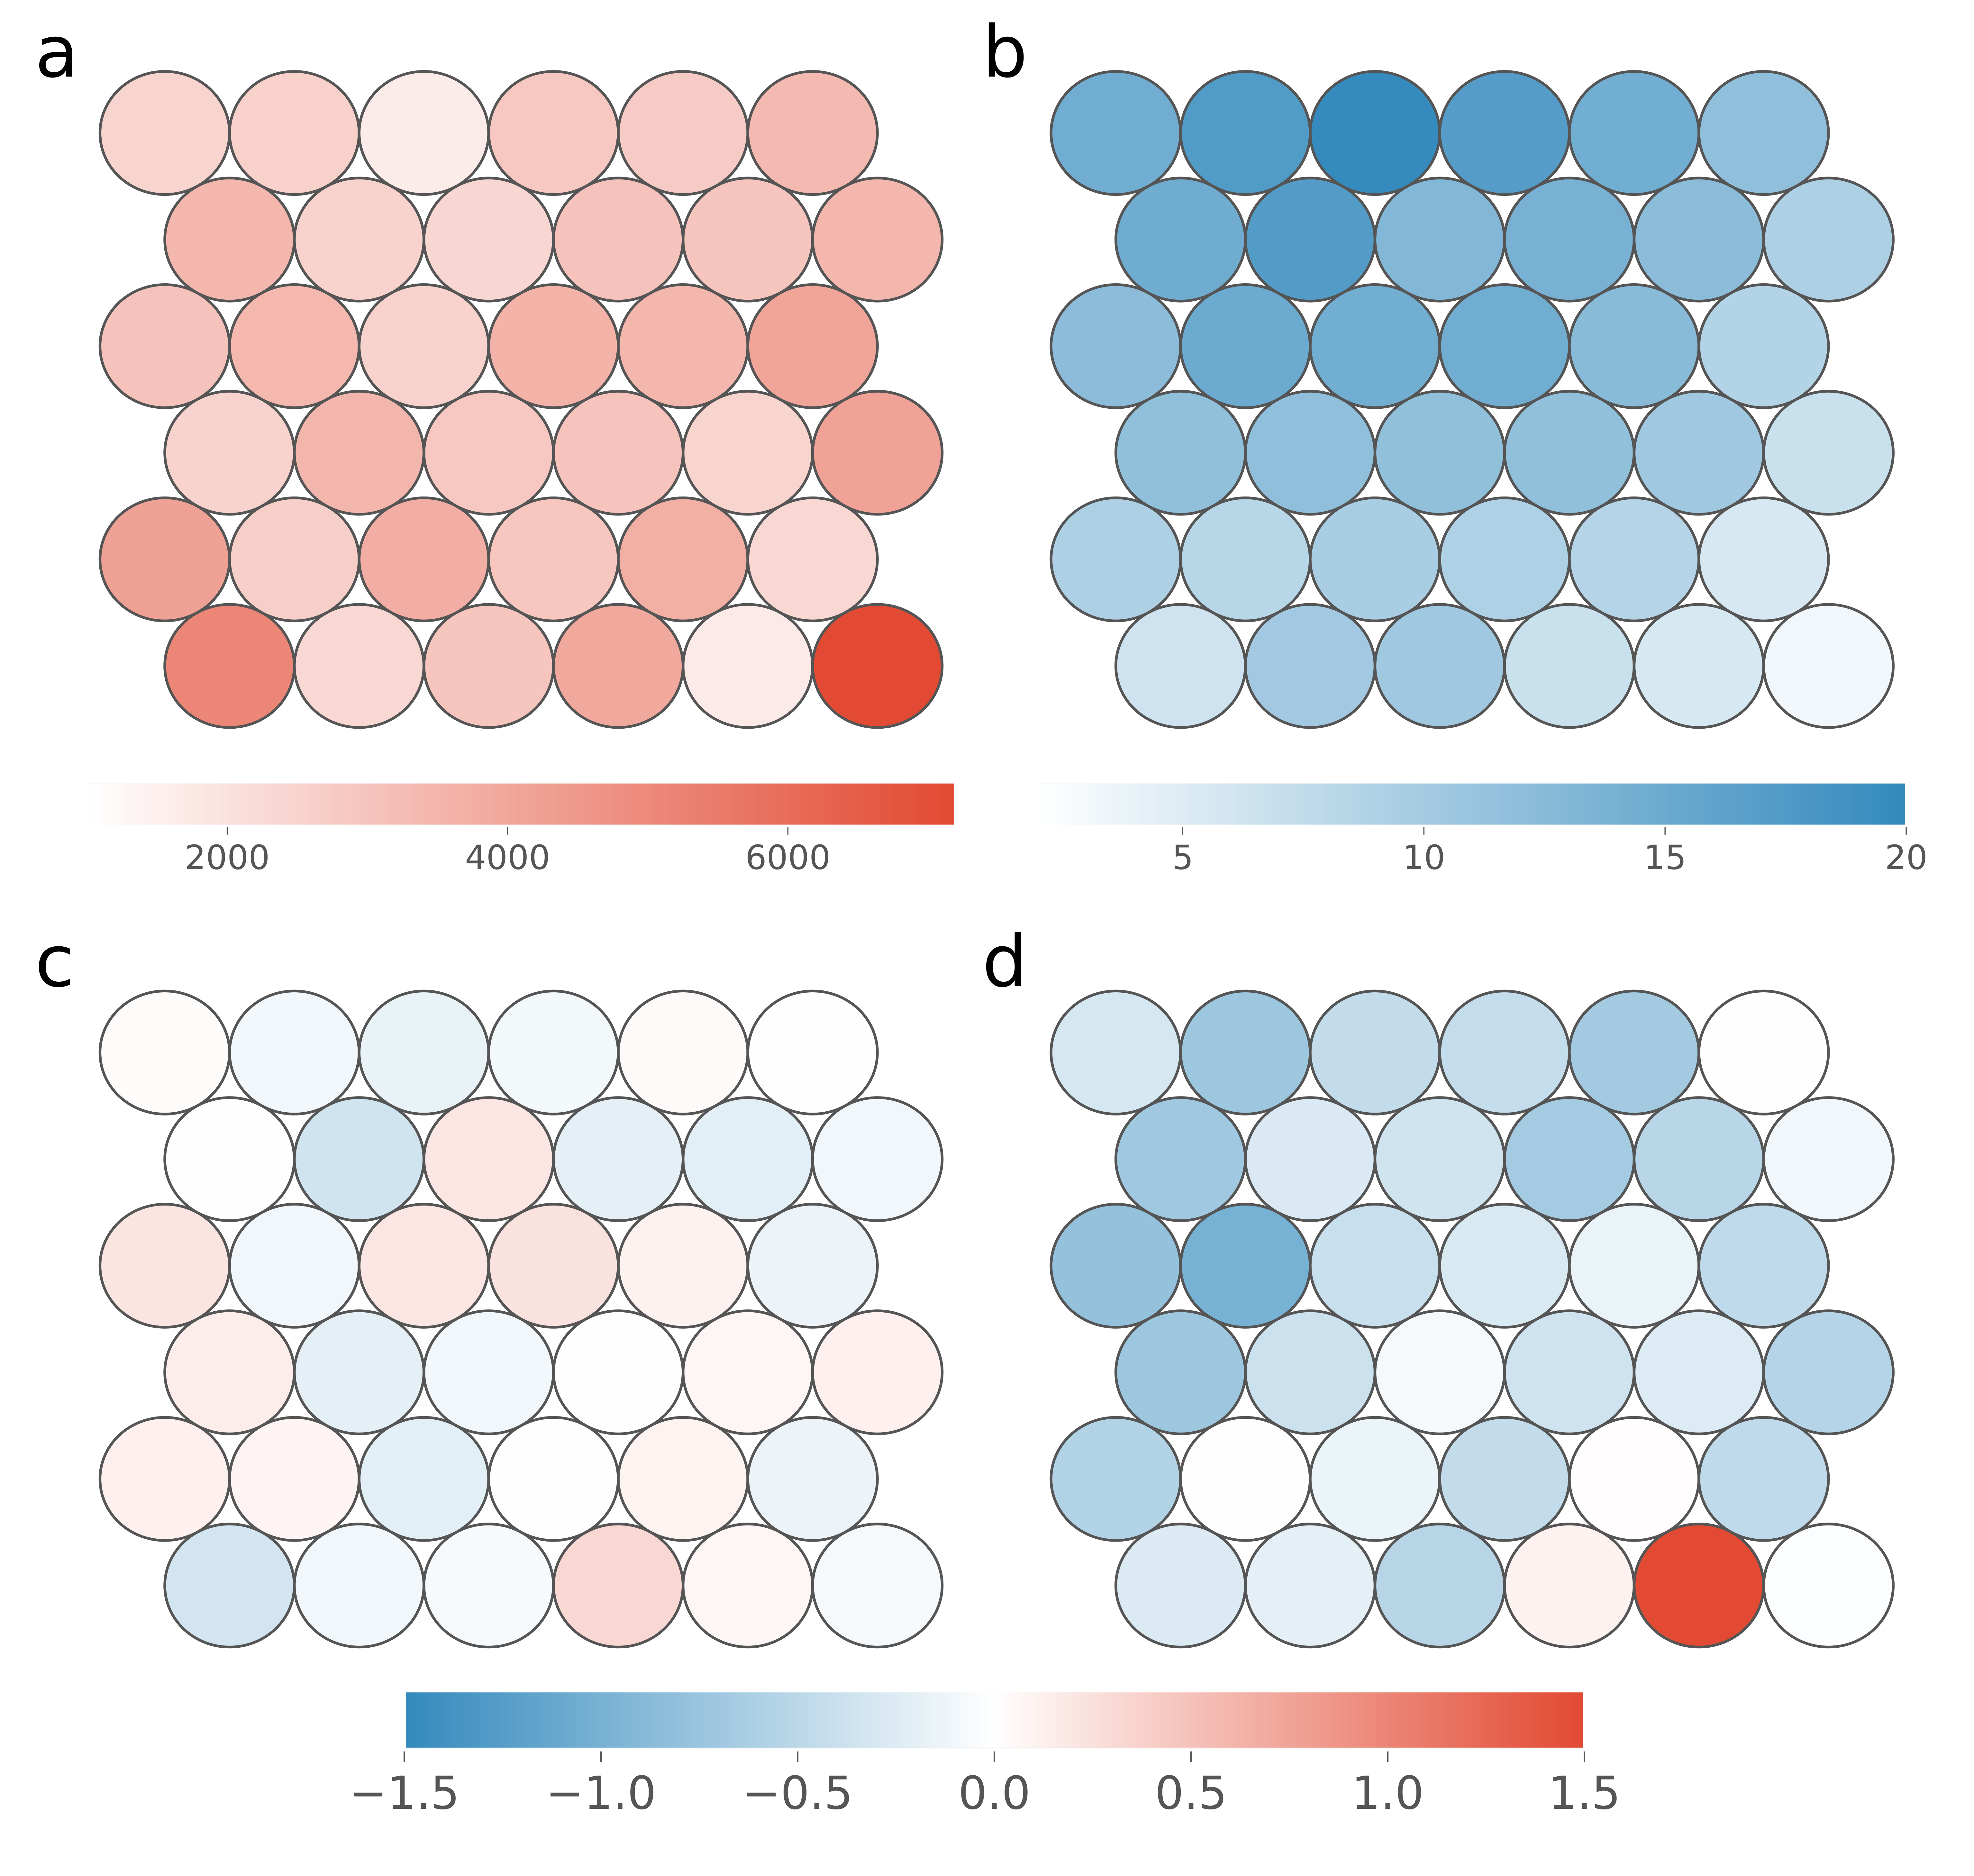
\includegraphics[width=\textwidth,height=562pt,keepaspectratio]{chapter_5/figures/som_enrichment.png}
\caption[Self Organising Maps demonstrate NMM downregulated genes contain specific PG4 types.]{\textbf{Self   Organising   Maps   demonstrate   NMM   downregulated   genes   contain   specific   PG4   types.}   Self   Organising   Map   (SOM)   plots   for   clustering   of   Quadparser   predicted   two   tetrad   PG4s   by   loop   length.   In   each   figure,   each   circle   represents   a   cluster   of   similar   PG4s.   \textbf{a)}   SOM   plot   coloured   by   cluster   size.   Each   cluster   contained   between   1000   and   8000   PG4s.   \textbf{b)}   SOM   plot   coloured   by   total   length   in   bases   of   all   loops.   \textbf{c)}   and   \textbf{d)}   Log2   fold   enrichment   of   each   cluster   in   the   gene   bodies   of   genes   downregulated   by   NMM,   on   the   coding   and   template   strands,   respectively.   Log2   fold   enrichments   were   generated   by   comparing   actual   overlap   of   PG4s   with   downregulated   genes,   with   expected   overlap   when   PG4s   were   permuted   amongst   all   genes.   \label{som}}
\end{figure}

\newpage

\hypertarget{nmm-downregulation-is-correlated-with-maximal-g4-density}{%
\subsection{NMM downregulation is correlated with maximal G4
density}\label{nmm-downregulation-is-correlated-with-maximal-g4-density}}

Previous studies have suggested that G4s cause the largest effect on
gene expression when grouped in clusters (Yoshida et al., 2018). This
may be due to an increase in the likelihood of a single G4 being formed
at any one time, or through increased polymorphy of G4 formation. To
identify whether NMM regulated genes tend to contain G4 clusters, we
used a sliding window of 200bp to count two tetrad G4 density across the
whole transcribed region of each gene, including introns. Each gene was
then assigned the maximum density score for the gene. Genes were then
binned by their maximal density, and expression under NMM was calculated
(Fig. \ref{max_g4}). We found that genes with higher maximal G4 density
tended to have more negative log fold changes during NMM treatment. This
suggests that clusters of G4s do have a stronger effect on gene
expression, and that a single region of high G4 density may be
sufficient to cause downregulation of an otherwise G4 free gene during
NMM treatment.

\newpage

\begin{figure}[htbp]
\centering
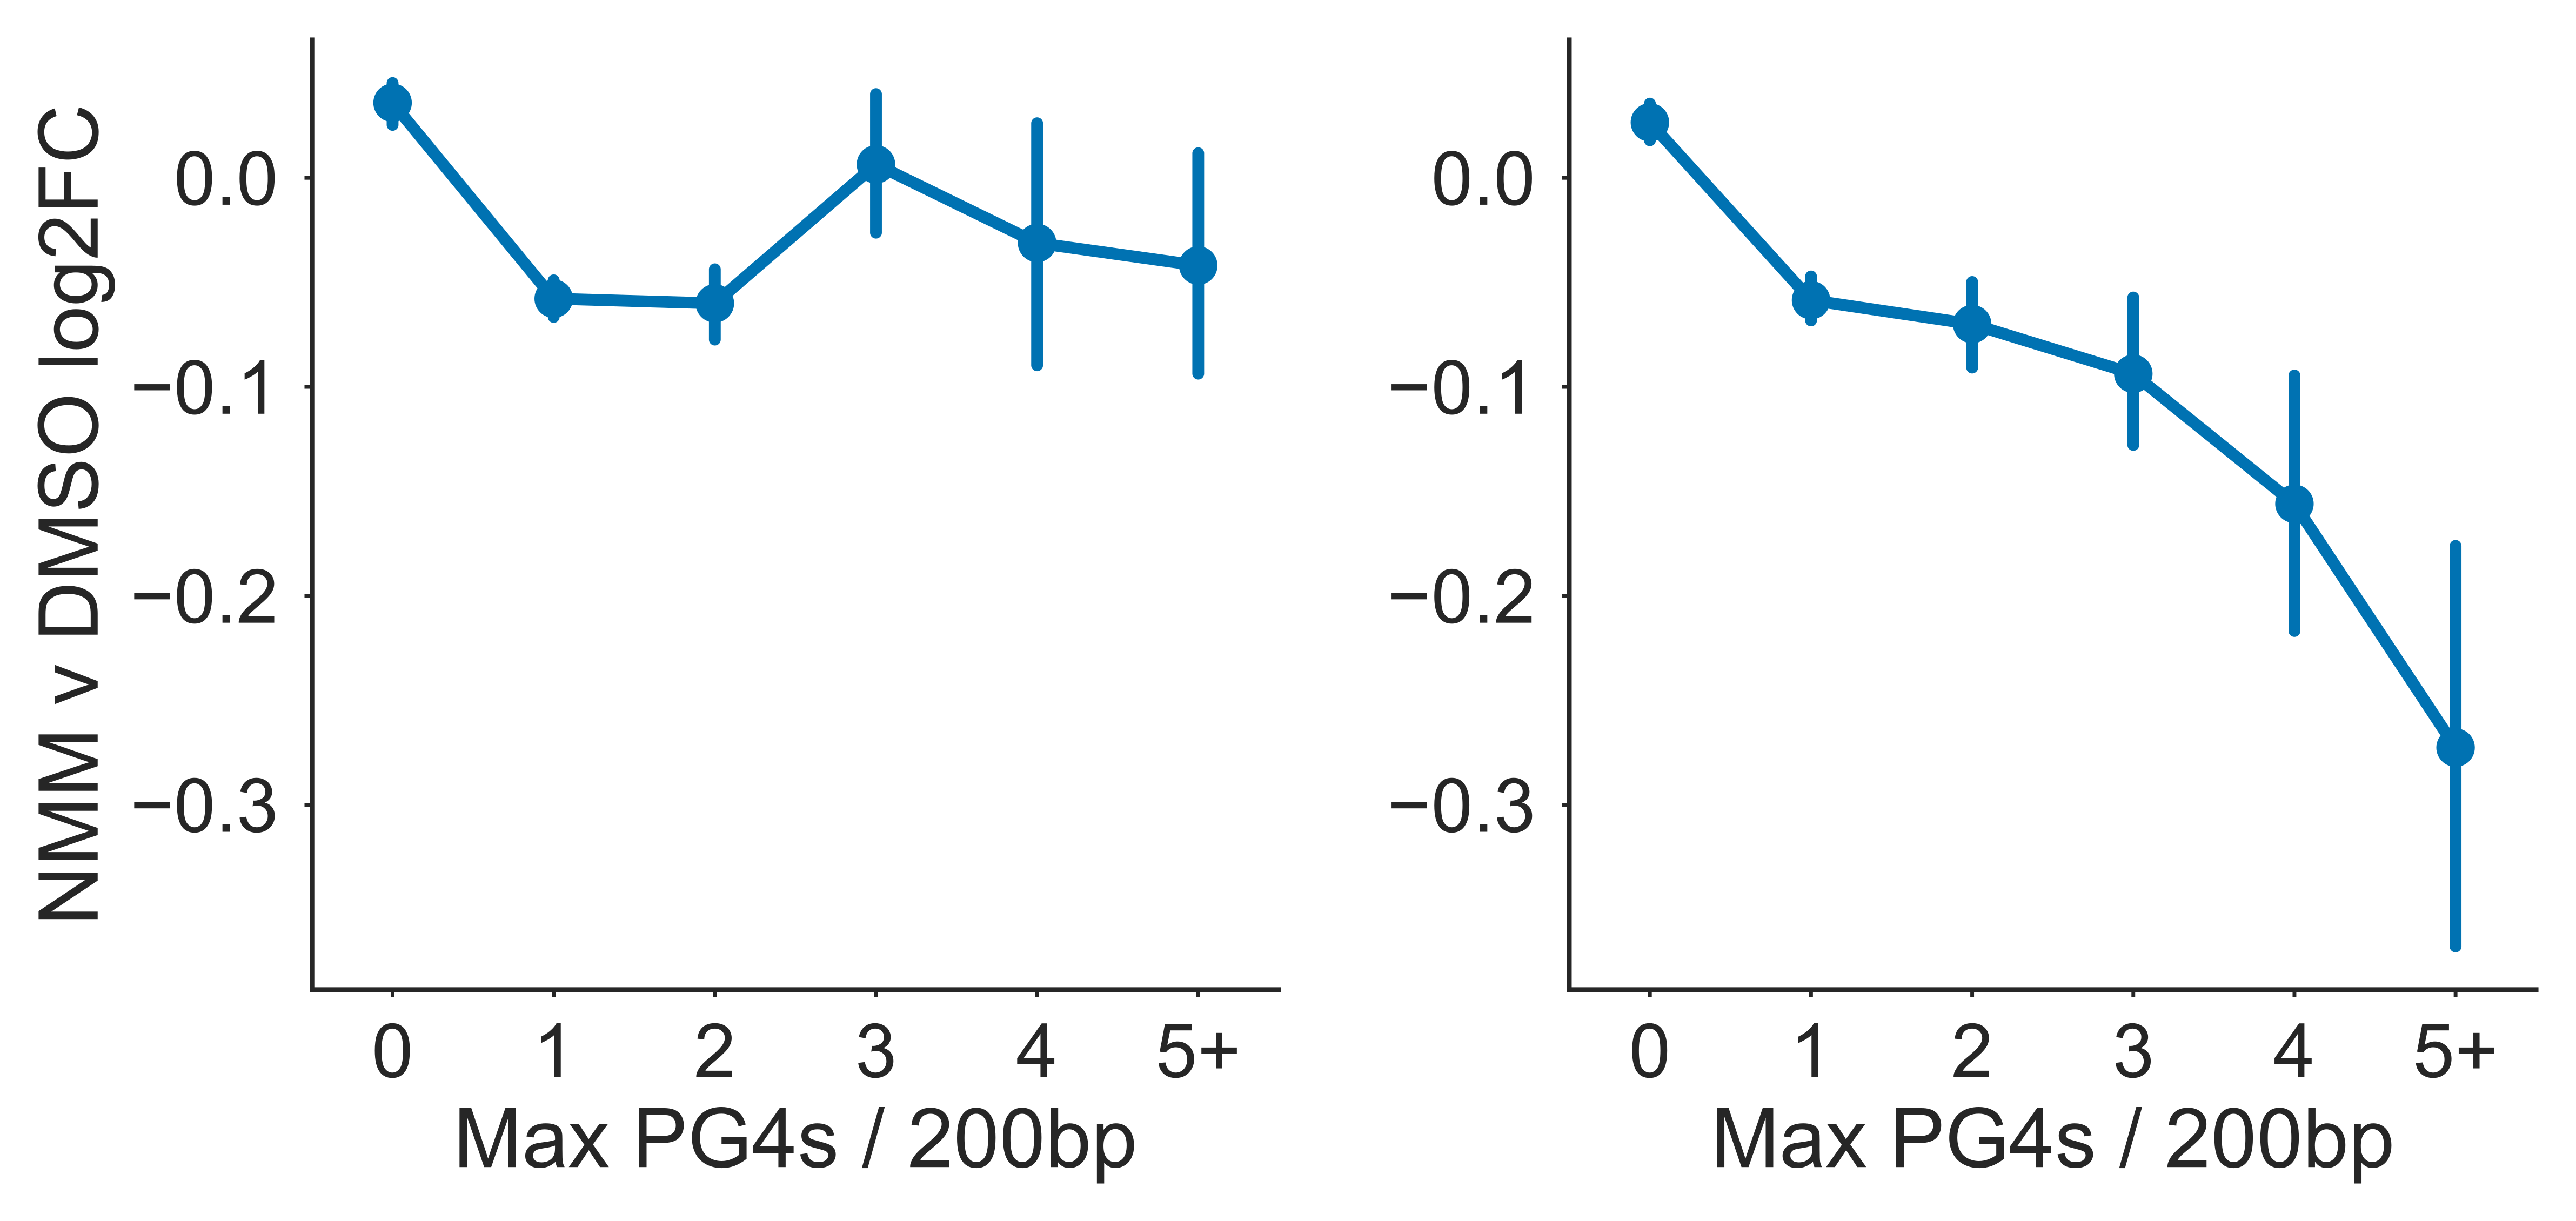
\includegraphics[width=\textwidth,height=562pt,keepaspectratio]{chapter_5/figures/nmm_exprs_g4_max_density.png}
\caption[NMM regulates genes with large maximal PG4 density]{\textbf{NMM   regulates   genes   with   large   maximal   PG4   density}   Point   plot   showing   mean   log   fold   change   in   gene   expression   during   NMM   treatment   for   genes   binned   by   " maximal   PG4   density ,   defined   as   the   greatest   concentration   of   PG4   motifs   within   a   200bp   sliding   window   anywhere   in   the   body   of   the   gene   (i.e. exon   or   intron).   Left   and   right   panels   depict   coding   and   template   strands,   respectively.   Errorbars   are   68\%   confidence   intervals   for   mean   generated   using   1000   bootstrapped   samples.   \label{max_g4}}
\end{figure}

\newpage

\hypertarget{g-quadruplexes-may-cause-downregulation-by-pol-ii-stalling}{%
\subsection{G Quadruplexes may cause downregulation by Pol II
stalling}\label{g-quadruplexes-may-cause-downregulation-by-pol-ii-stalling}}

Since transcriptional downregulation by NMM stabilised G4s appears to
occur most strongly for genes which have many G4s in the gene body, and
because this effect is specific to the template strand, we hypothesised
that this could be a result of RNA Polymerase (Pol II) stalling. Pol II
is the RNA polymerase which is responsible for transcribing all protein
coding genes. The Pol II complex scans along the template strand and
uses complementary base pairing to produce an mRNA copy which
corresponds to the sequence of the coding strand. Since only the
template strand is read directly, this might explain why coding strand
G4s do not cause downregulation, since they do not form blockages which
prevent the elongation of Pol II. To test whether G4s cause blockages
which slow or stall the elongation of Pol II in the abscence of
stabilisation by NMM, we reanalysed Pol II ChIP tiling array data
(Chodavarapu et al., 2010). Metagene profiles of the transcriptional
start and end sites showed an accumulation of Pol II at the
transcriptional termination site (TTS) (Fig \ref{pol_ii}, orange
profiles). This was surprising as it is in disagreement with Pol II
occupancy profiles in human cell lines, where there is generally a much
larger peak of paused Pol II at the start of the gene. We contrasted
this result with occupancy profiles for G4 dense genes (Fig
\ref{pol_ii}, blue profiles). For genes which contained at least one G4
dense region, measured either by G4Seeqer score greater than 0.95, or by
maximum Quadparser G4 density per 200bp of greater than 3, we found that
there was greater Pol II occupancy at the TSS and in the TSS proximal
part of the gene body. Greater Pol II occupancy can be explained by
either of two factors: increased initiation and transcription in G4
dense genes, or slower Pol II elongation. Since G4 dense genes do not
have higher expression than non-G4 containing genes, we suggest that
template strand G4s cause a reduction in Pol II speed. This may result
in abortive transcription or alteration of co-transcriptional processes
such as splicing.

\newpage

\begin{figure}[htbp]
\centering
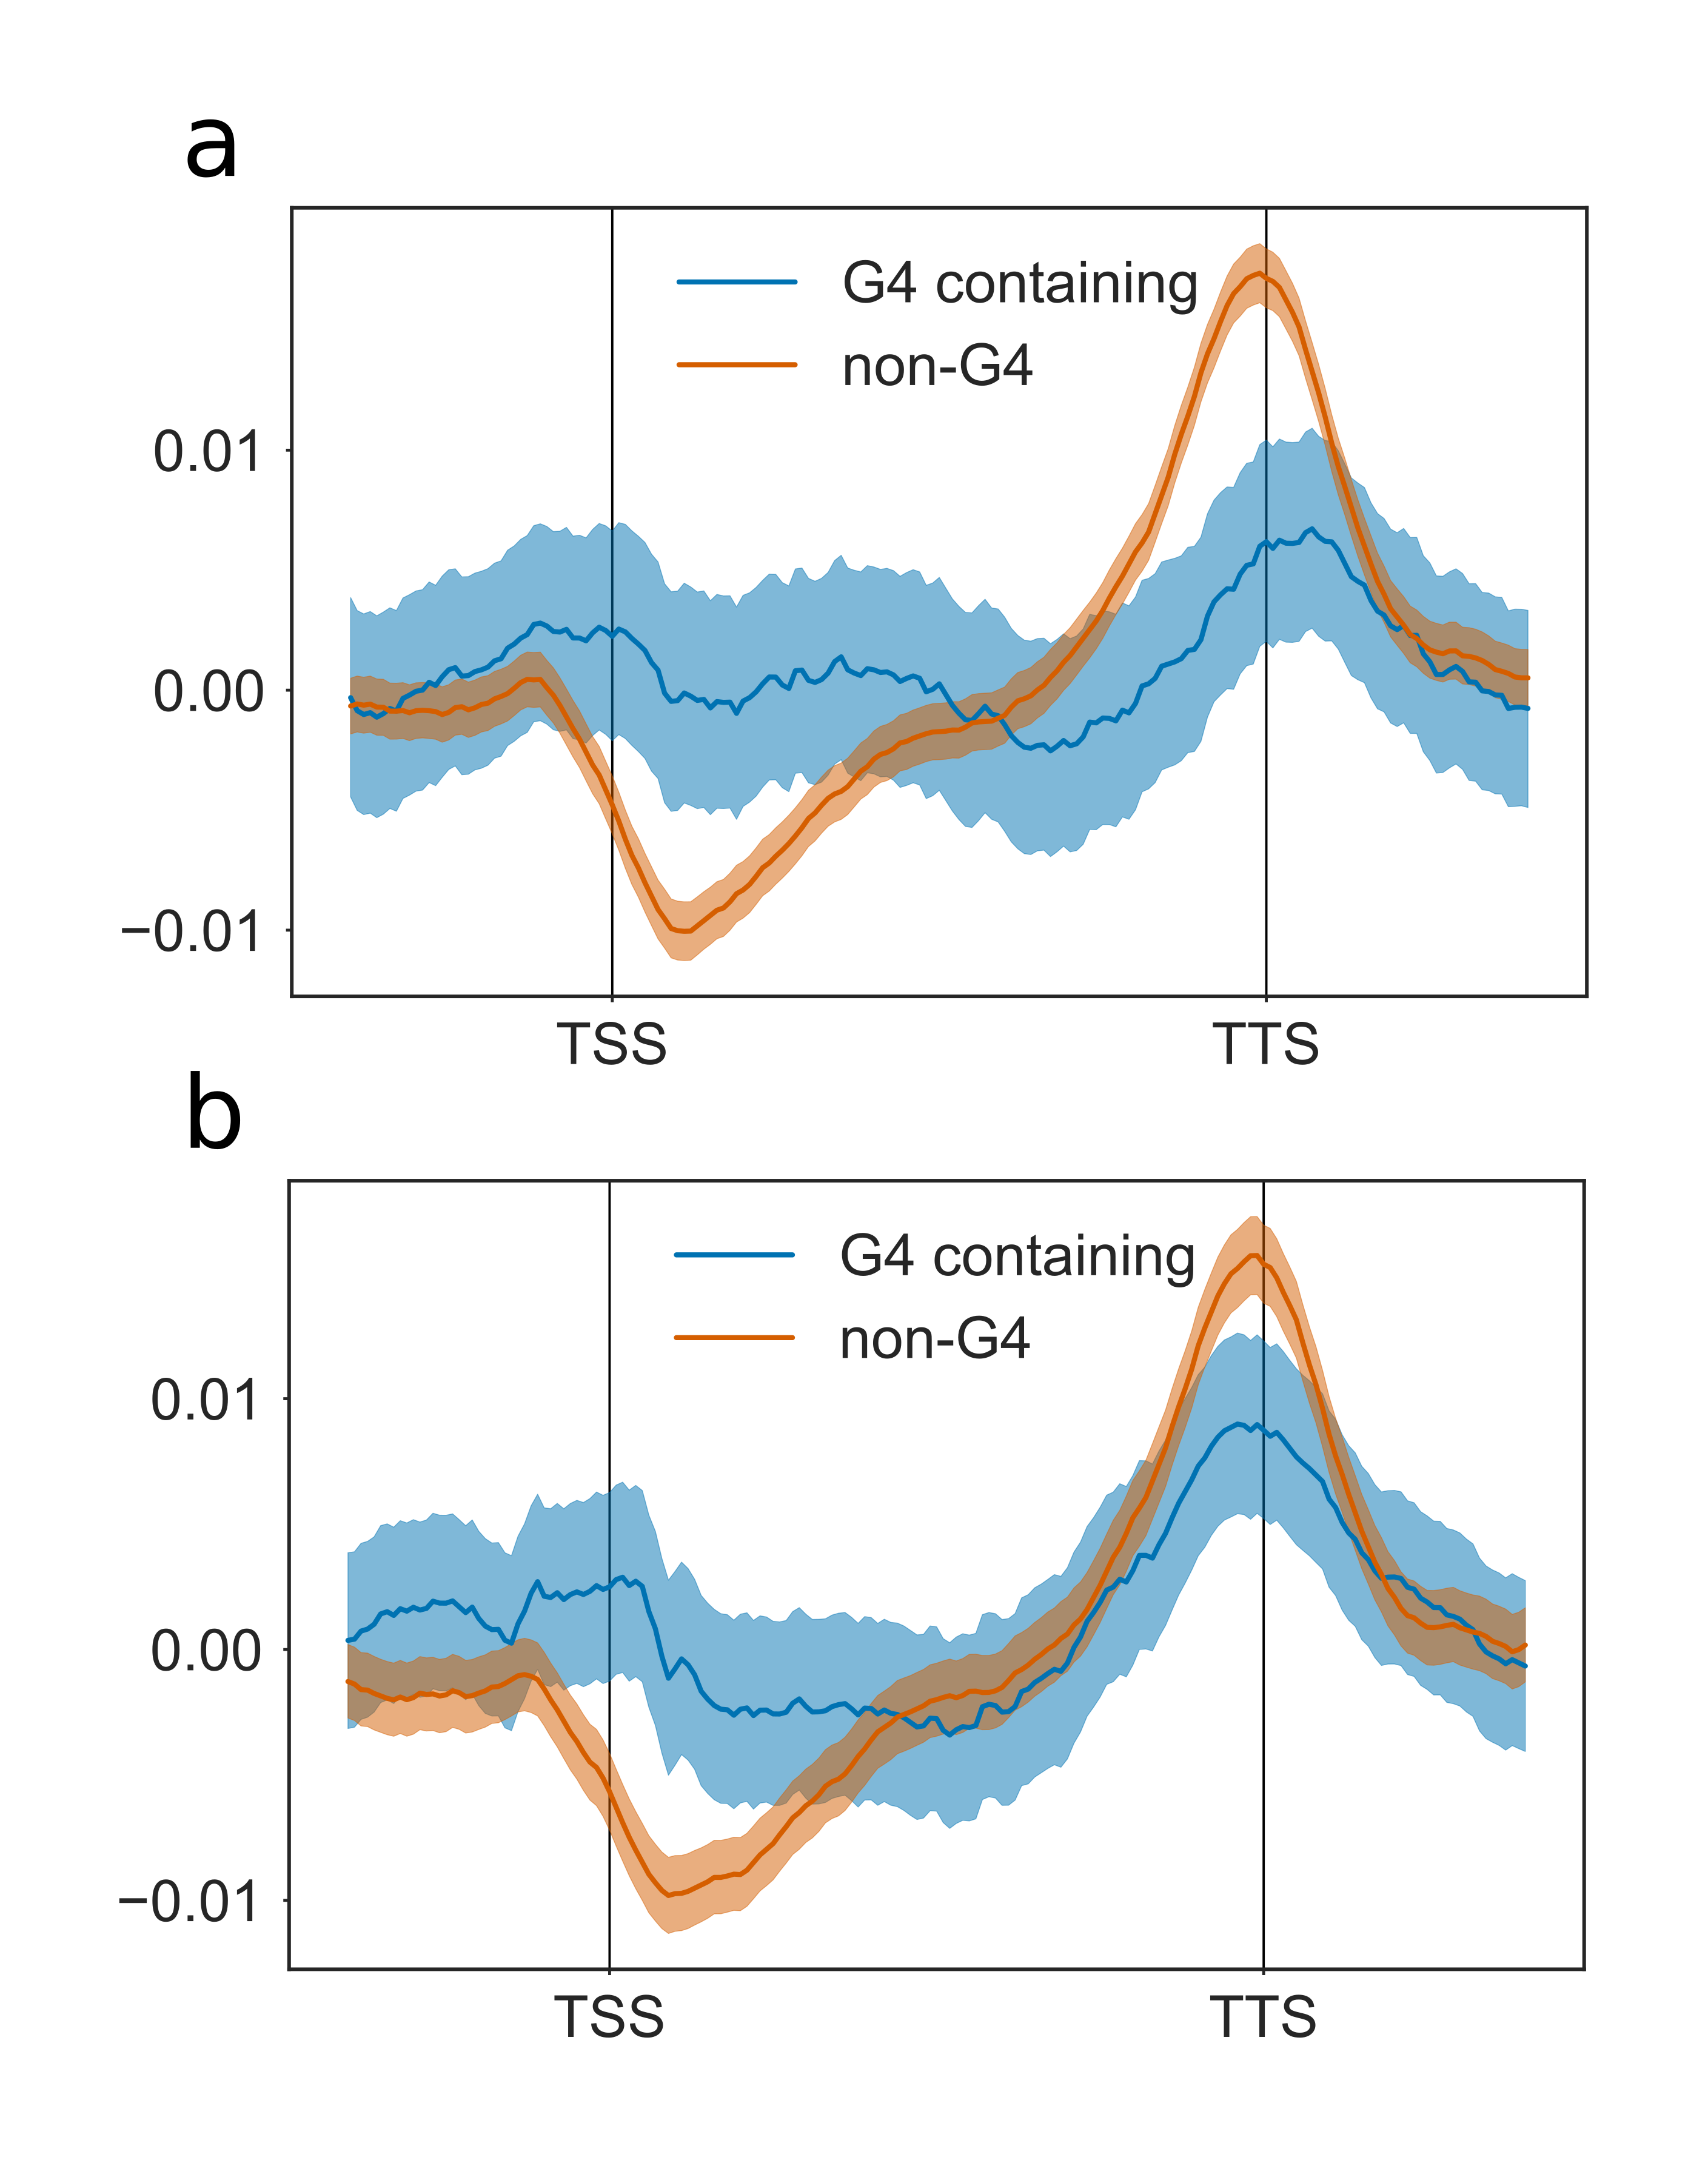
\includegraphics[width=\textwidth,height=562pt,keepaspectratio]{chapter_5/figures/polii_occupancy.png}
\caption[PG4 dense genes have altered RNA Polymerase II occupancy]{\textbf{PG4   dense   genes   have   altered   RNA   Polymerase   II   occupancy}   Metagene   profiles   showing   RNA   Polymerase   II   (Pol   II)   occupancy   across   binned   exonic   gene   bodies.   Profiles   are   made   up   of   500bp   upstream   region   (in   10bp   bins),   100   gene   body   bins,   and   500bp   downstream   region   (in   10bp   bins).   \textbf{a)}   Metagene   profile   for   genes   containing   PG4   predicted   by   G4Seeqer   (max   G4seeqer   score   >   0.9),   vs. genes   containing   no   G4s   (max   G4seeqer   score   <   0.1).   \textbf{b)}   Metagene   profile   for   genes   containing   two   tetrad   maximal   PG4   density   per   200bp   of   3   or   greater,   vs. genes   with   maximal   PG4   density   of   zero   (contain   no   PG4s).   Averages   were   generated   using   1000   bootstrapped   samples   from   each   geneset.   Bootstrapped   samples   are   normalised   such   that   the   absolute   area   under   the   curve   was   equal   to   one.   Errorbars   are   68\%   confidence   intervals   for   bootstrapped   means.   \label{pol_ii}}
\end{figure}

\newpage

\hypertarget{g-quadruplex-stalling-may-result-in-abortive-transcription}{%
\subsection{G Quadruplex stalling may result in abortive
transcription}\label{g-quadruplex-stalling-may-result-in-abortive-transcription}}

To test whether template G4 containing genes might produce abortive
transcripts that are degraded by the exosome rather than maturing to
mRNAs, we analysed publicly available GRO-seq data (Hetzel et al.,
2016). Since GRO-seq captures nascent RNA irrespective of its stability,
and RNAseq captures stable RNAs, the ratio between the normalised read
counts in GROseq vs RNAseq represents an estimate of the amount of
unstable products produced at each gene locus (Fig. \ref{gro}a). We
found that the largest difference in ratio was between non-coding and
protein coding RNAs, with non-coding RNAs having much greater GRO/RNA
ratios (data not shown). This is likely explained by the higher rate of
modification of many ncRNAs, e.g.~tRNAs, which prevent reverse
transcription and sequencing by RNAseq. Other ncRNAs such as natural
antisense RNAs may also be unstable and degraded quickly.

G4 predictions were calculated using G4Seeqer and the score of the
maximum score region within the transcribed body of each gene was
assigned to the gene. A G4 containing set was produced using genes which
contained a maximum template strand G4seeqer score of more than 0.95,
and a G4 negative set was produced using genes with a maximum score of
only 0.05 or less. We found a small but significant positive increase in
GRO/RNA ratio for G4 dense genes (p = 0.009), suggesting that some
abortive transcripts are produced from these genes (Fig. \ref{gro}b,
right panel). In contrast, genes with high scoring G4 regions on the
coding strand did not have greater GRO/RNA ratios (p=0.4) (Fig.
\ref{gro}b, left panel).

We conducted the same analysis using genes containing three or more two
tetrad PG4s in 200bp maximal density clusters, as described above (Fig.
\ref{gro}c). For these genes, we did not find any significant increase
in GRO/RNA ratio, suggesting that these two tetrad G4s are not
sufficiently stable to cause abortive transcription. Since these genes
do have higher promoter proximal Pol II occupancy, we suggest that
elongation occurs more slowly across the genes, but does not cause
premature termination.

\newpage

\begin{figure}[htbp]
\centering
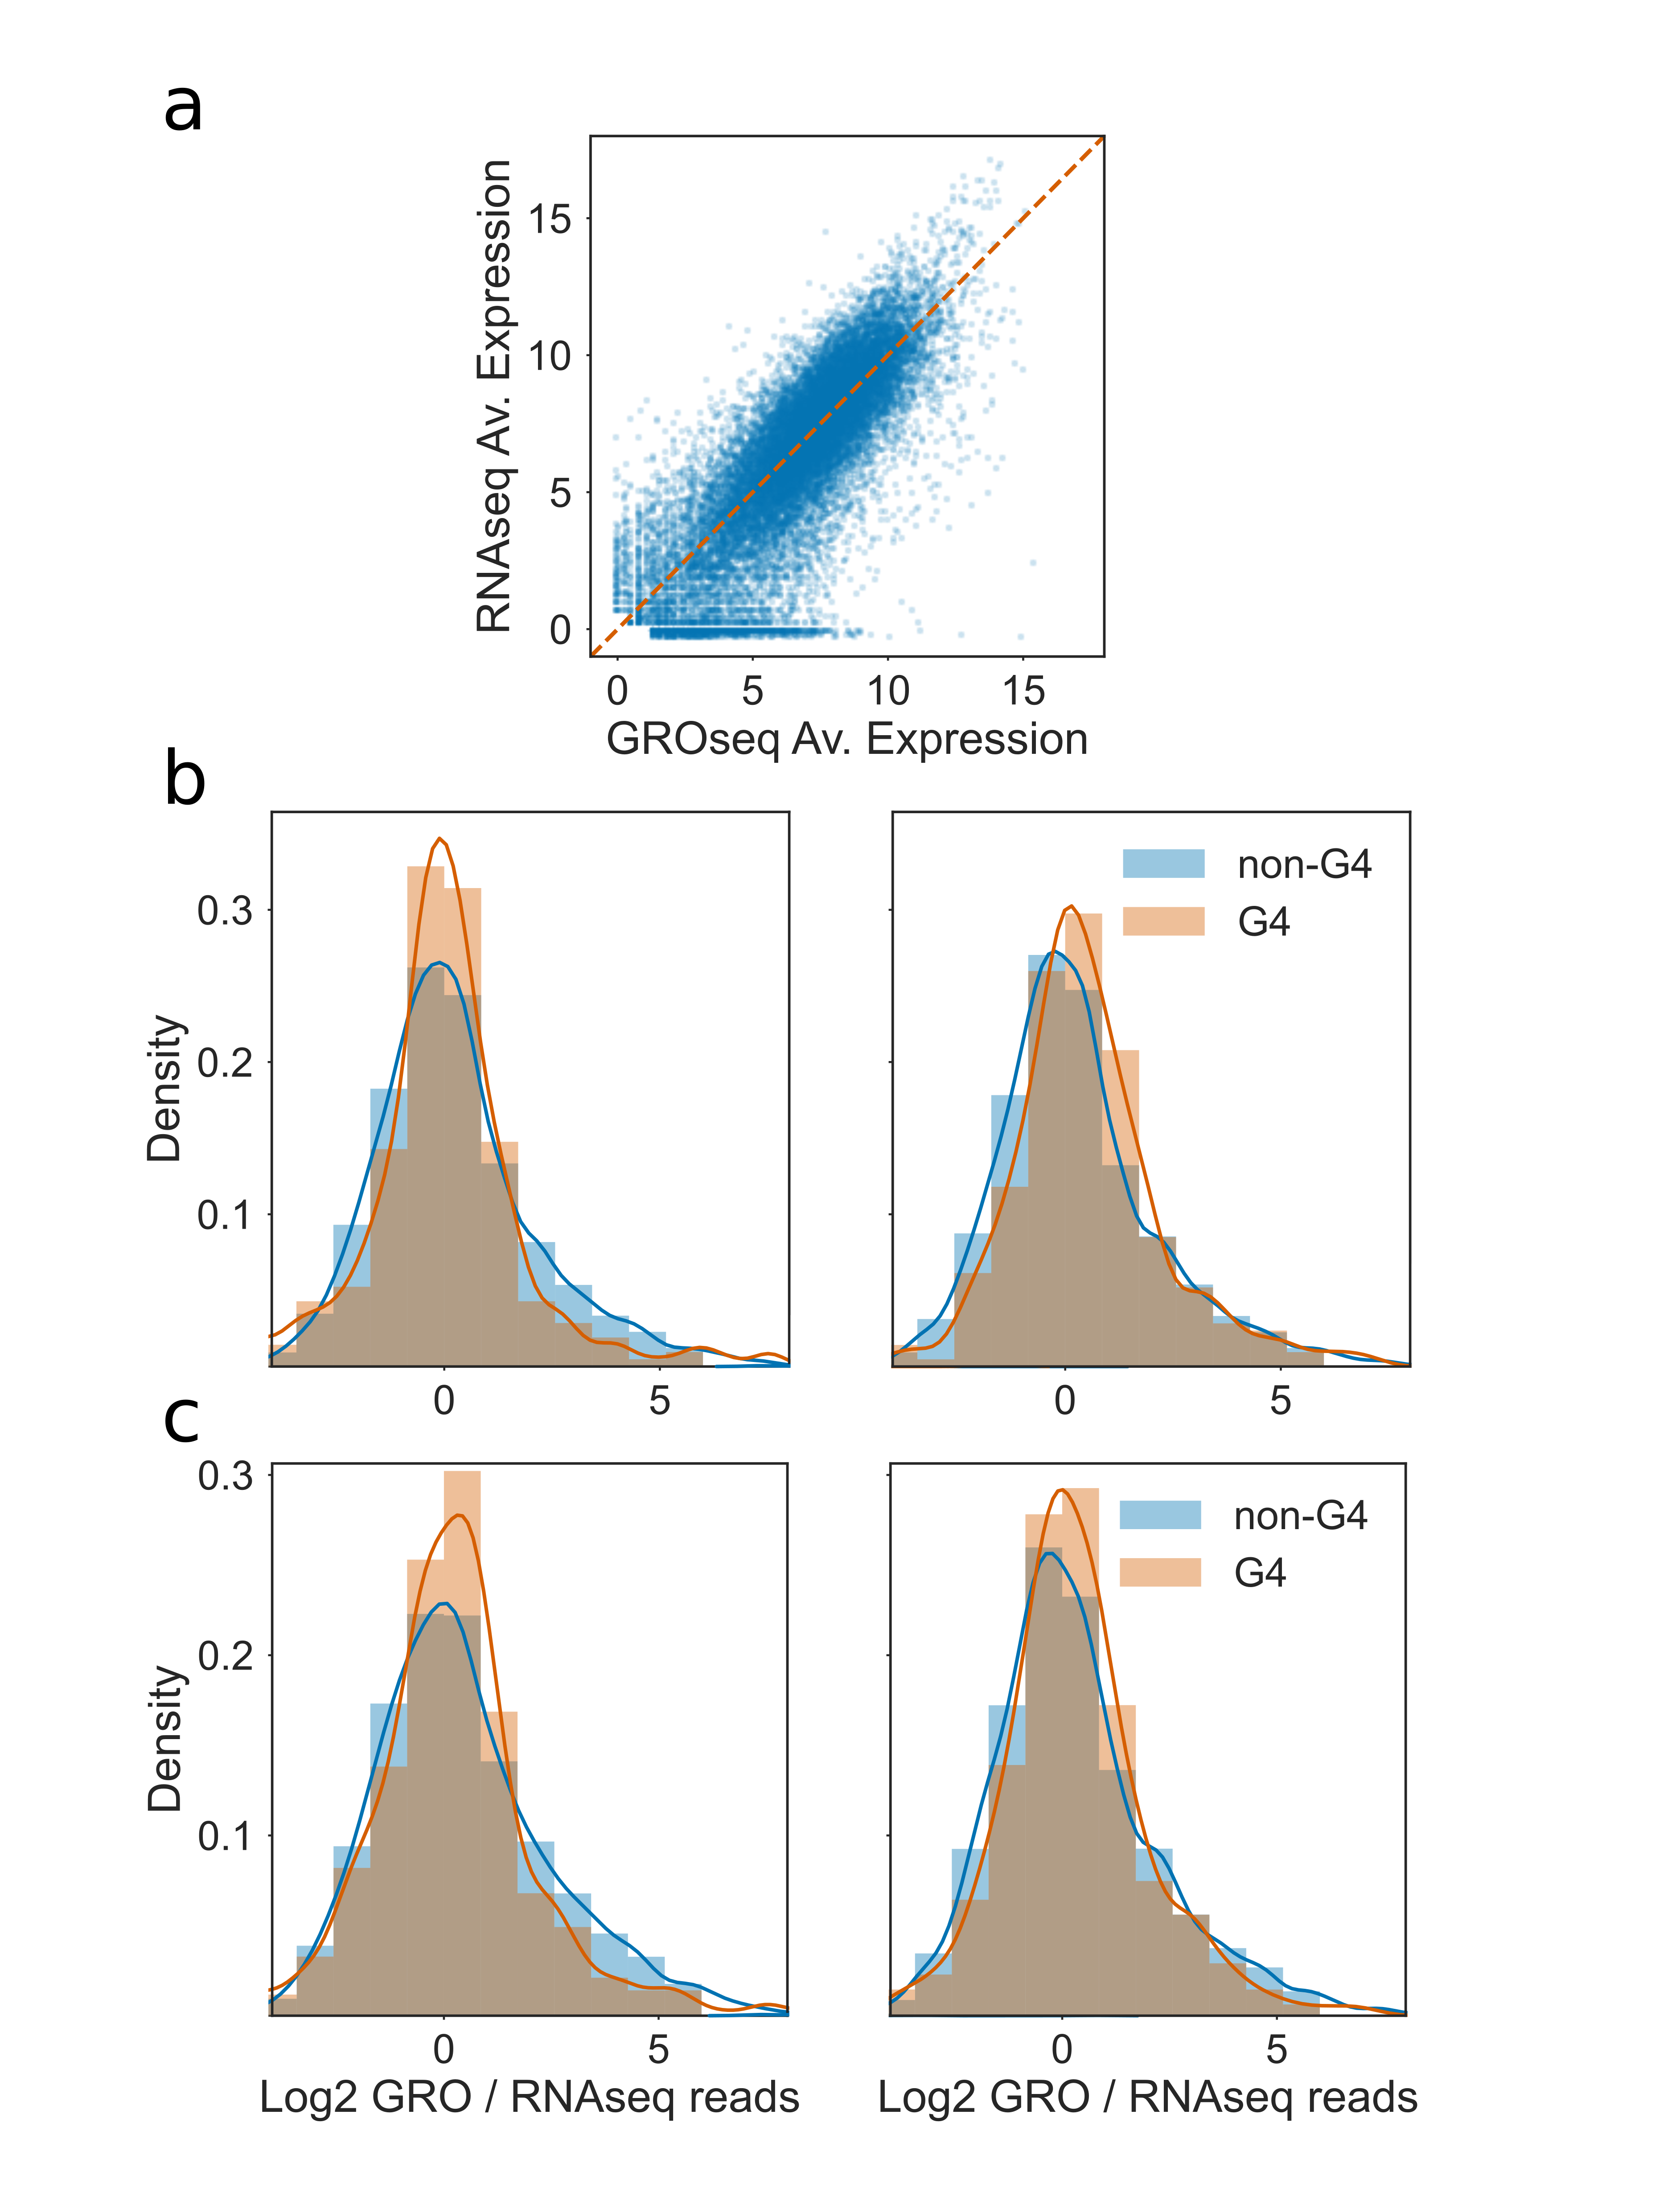
\includegraphics[width=\textwidth,height=562pt,keepaspectratio]{chapter_5/figures/gro_g4s.png}
\caption[Log Ratio of GRO / RNA seq counts per million detects abortive transcription of PG4 dense genes.]{\textbf{Log   Ratio   of   GRO   /   RNA   seq   counts   per   million   detects   abortive   transcription   of   PG4   dense   genes.}   \textbf{a)}   Scatter   plot   showing   measured   expression   in   log2   counts   per   million   (logCPM)   for   each   gene   from   GRO-seq   vs. RNAseq   datasets.   Genes   which   fall   below   and   to   the   right   of   the   orange   line   have   positive   log2   GRO/RNA   ratios.   \textbf{b)}   Histogram   and   kernel   density   estimates   of   GRO/RNA   ratio   for   genes   containing   PG4   predicted   by   G4Seeqer   (max   G4seeqer   score   >   0.9)   in   orange,   vs. genes   containing   no   G4s   (max   G4seeqer   score   <   0.1)   in   blue.   Left   and   right   panels   represent   coding   and   template   strand   G4   rich   genes,   respectively.   \textbf{c)}   Histogram   and   kernel   density   estimates   of   GRO/RNA   ratio   for   genes   containing   two   tetrad   maximal   PG4   density   per   200bp   of   3   or   greater   in   orange,   vs. genes   with   maximal   PG4   density   of   0   (contain   no   PG4s)   in   blue.   Left   and   right   panels   represent   coding   and   template   strand   G4   rich   genes,   respectively.   \label{gro}}
\end{figure}

\newpage

\hypertarget{nmm-treatment-does-not-activate-dna-damage-response-pathways}{%
\subsection{NMM treatment does not activate DNA damage response
pathways}\label{nmm-treatment-does-not-activate-dna-damage-response-pathways}}

Rodriguez et al.~showed that treatment of human cells with Pyridostatin
(PDS), a G4 binding agent, caused an increase in the histone marker
γH2AX, which is associated with double stranded DNA breaks (Rodriguez et
al., 2012). Cells in gap phases 1 \& 2, during which DNA is not being
replicated, showed a reduction in double strand breaks when also treated
with 5,6-dichloro-1-β-D-ribofuranosylbenzimidazole, an inhibitor of
transcription. This suggests that PDS causes transcription and
replication dependent DNA damage, presumably resulting from Pol II and
replication fork stalling at G4 loci. To see if NMM causes similar DNA
damage in \emph{Arabidopsis thaliana}, we looked for transcriptional
signatures of damage response. A set of 7 genes: AGO2, PARP1, RPA1E,
BRCA1, GRG, RAD51, and RAD17, which have been reported as strong
transcriptional markers of DNA damage (Ryu et al., 2018) were tested.
Only AGO2 showed upregulation (logFC=1.23, PPLR=1) upon NMM treatment
(Fig. \ref{damage}a). We next compared data from a microarray in which
seedlings were treated with Gamma Irradiation so see if there was any
overlap with genes regulated by NMM. We found a small but significant
overlap in upregulated genes (P = 2.9e-29). Gene ontology analysis of
the overlapping gene set yielded no clear results, however. In
comparison, the total gamma irradiation upregulated set was strongly
enriched for genes involved in double strand break repair (FDR =
9.68e-4). Taken together, this data suggests that NMM treatment does not
cause major DNA instability or DNA damage response.

\newpage

\begin{figure}[htbp]
\centering
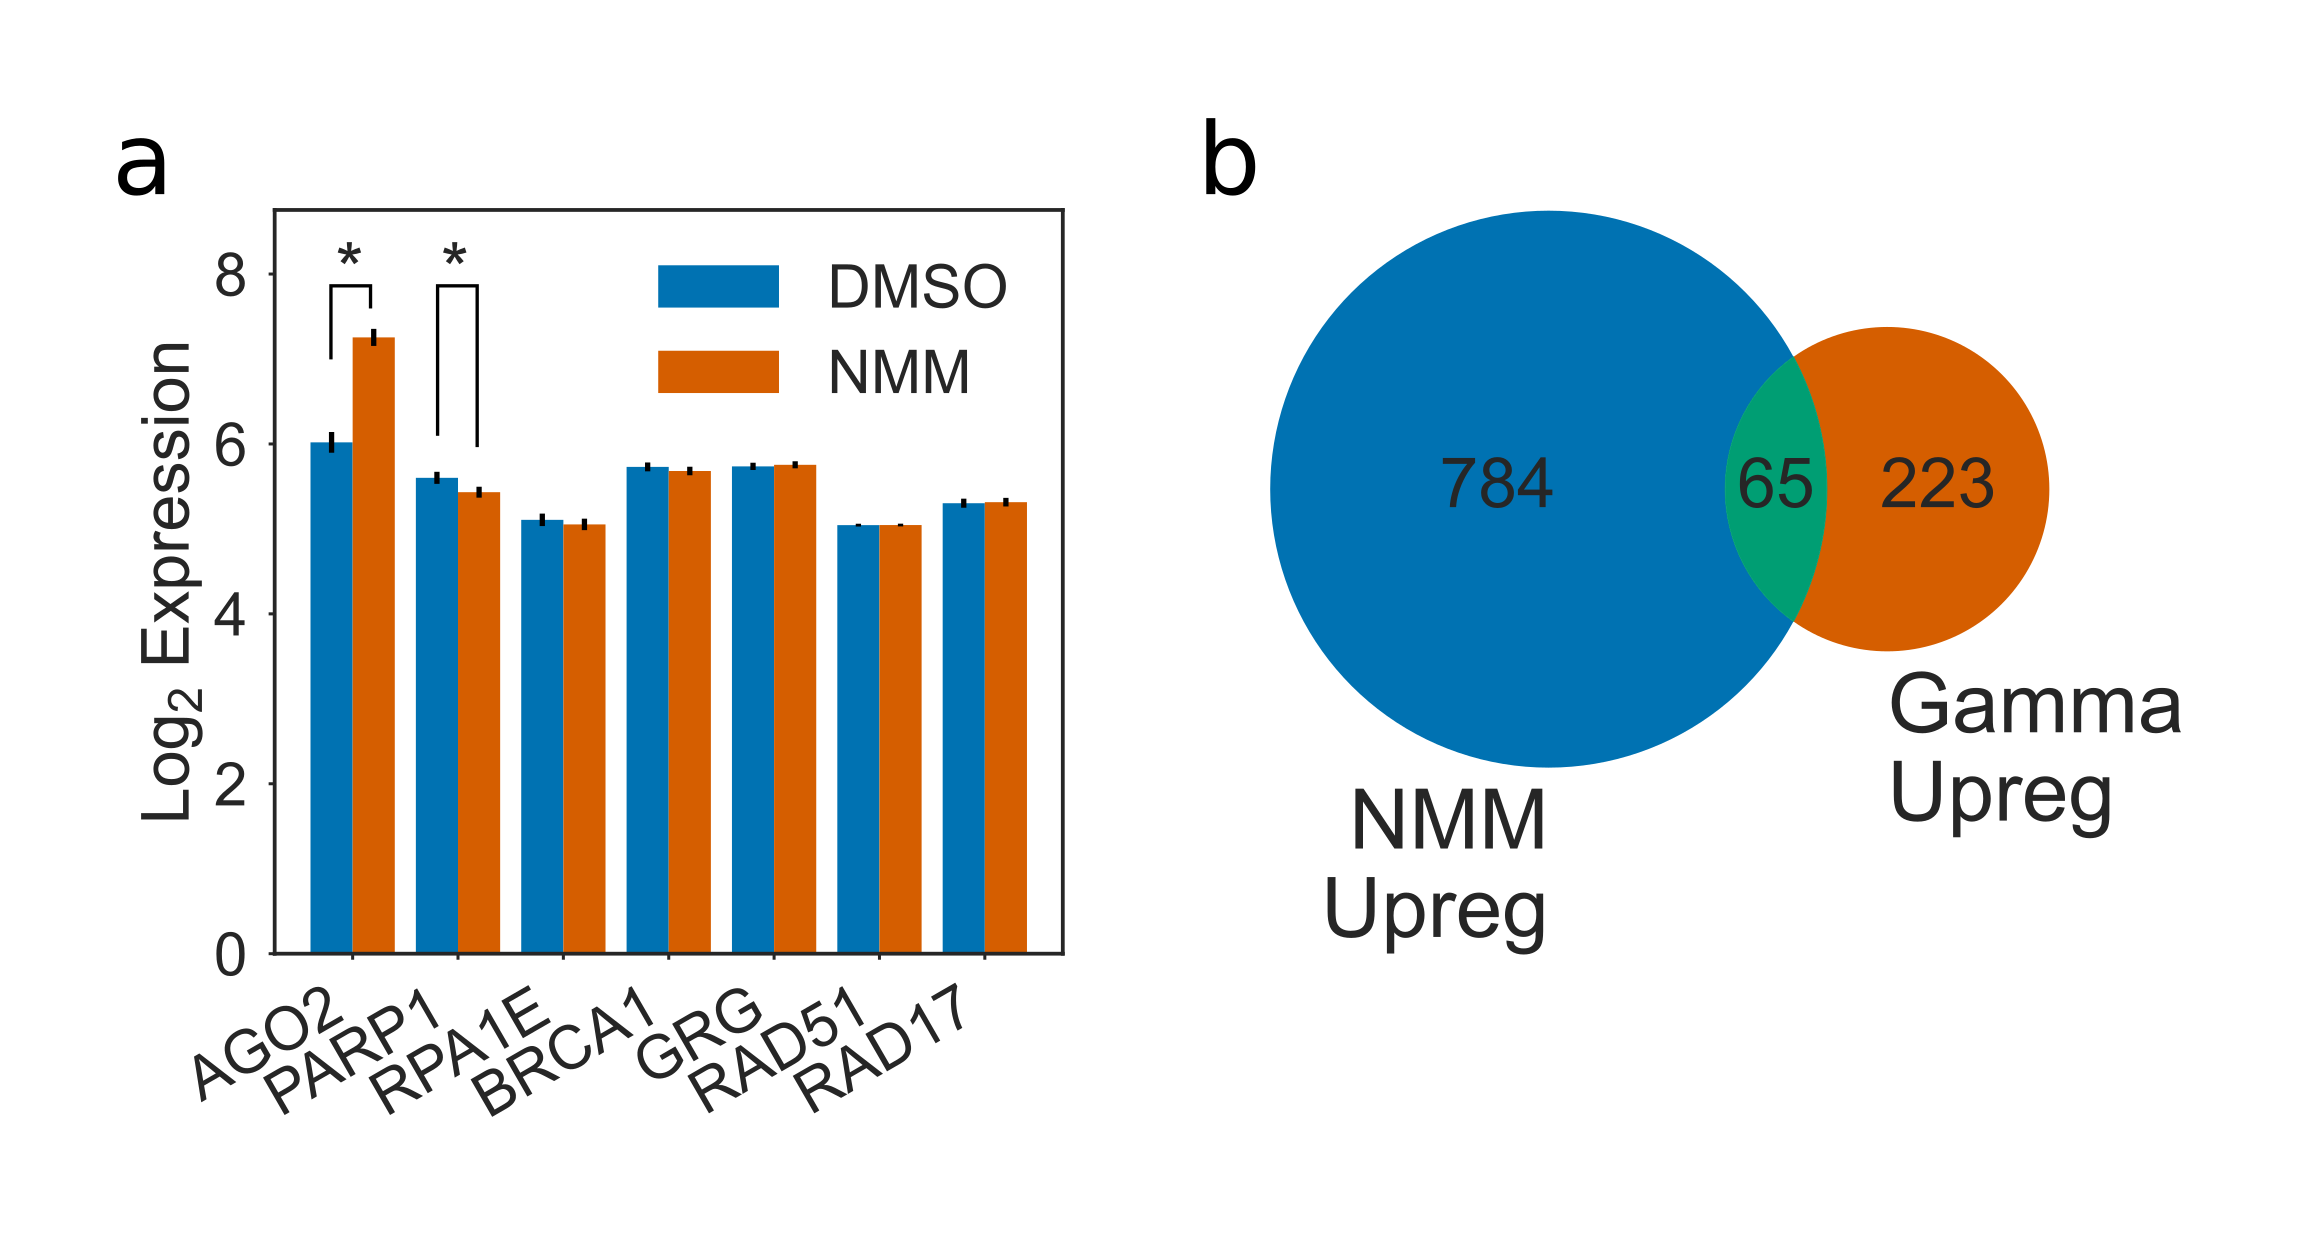
\includegraphics[width=\textwidth,height=562pt,keepaspectratio]{chapter_5/figures/dna_damage_response.png}
\caption[NMM does not activate DNA damage response]{\textbf{NMM   does   not   activate   DNA   damage   response}   \textbf{a)}   Barplot   showing   normalised   log2   expression   of   seven   DNA   damage   responsive   genes:   AGO2,   PARP1,   RPA1E,   BRCA1,   GRG,   RAD51,   and   RAD17,   in   the   presence   and   absence   of   NMM.   Errorbars   are   standard   errors   calculated   by   \texttt{puma} .   Asterisks   denote   significant   results.   \textbf{b)}   Venn   diagram   showing   the   overlap   between   NMM   upregulated   genes   and   genes   upregulated   in   response   to   gamma   irradiation.   \label{damage}}
\end{figure}

\newpage

\hypertarget{g4-dense-genes-are-modulated-by-environmental-stress-and-correlate-with-nmm-treatment}{%
\subsection{G4 dense genes are modulated by environmental stress and
correlate with NMM
treatment}\label{g4-dense-genes-are-modulated-by-environmental-stress-and-correlate-with-nmm-treatment}}

Because G4s require potassium cations or other divalent cations for
formation, it has been noted by previous studies that they might form
more readily under stress conditions in plants such as drought stress,
when the intracellular concentrations of such ions is increased (Mullen
et al., 2010, 2012). Mullen et al.~showed that genes involved in
response to drought stress tended to be more likely to contain
G-Quadruplexes in their gene bodies. To more closely examine this
hypothesis we reanalysed microarrays conducted using RNA from drought
stressed plants (Linster et al., 2015) to determine whether
differentially expressed genes contained enrichments or depletion of PG4
structures within various gene regions. As with experiments conducted on
the NMM microarray, genes were considered to be moderately
differentially expressed if they underwent a log change in expression of
greater than 0.5 fold (FDR \textless{} 0.05). Genes which changed in
expression by more than 1 log fold (FDR \textless{} 0.05) were
considered strongly differentially expressed. 2947 and 491 genes showed
moderate or strong upregulation, respectively, and 2572 and 984 genes
showed moderate or strong downregulation. These gene sets were then
analysed for two tetrad G4 density using the Quadparser method. As with
NMM downregulated genes, we found that genes downregulated during
drought stress tended to have greater numbers of template strand PG4s in
exonic regions. Around 8\% more genes than expected contained at least
one template PG4 in the gene body (p=1e-11) (Fig \ref{drought_g4_sq}).
This enrichment appeared specifically in CDS and 5' UTR regions (Fig.
\ref{drought_g4}b-c). Interestingly, we also found that genes which were
upregulated during drought stress were more likely to have PG4s in the
coding strand of their 3' UTRs (Fig. \ref{drought_g4}d).

\newpage

\begin{figure}[htbp]
\centering
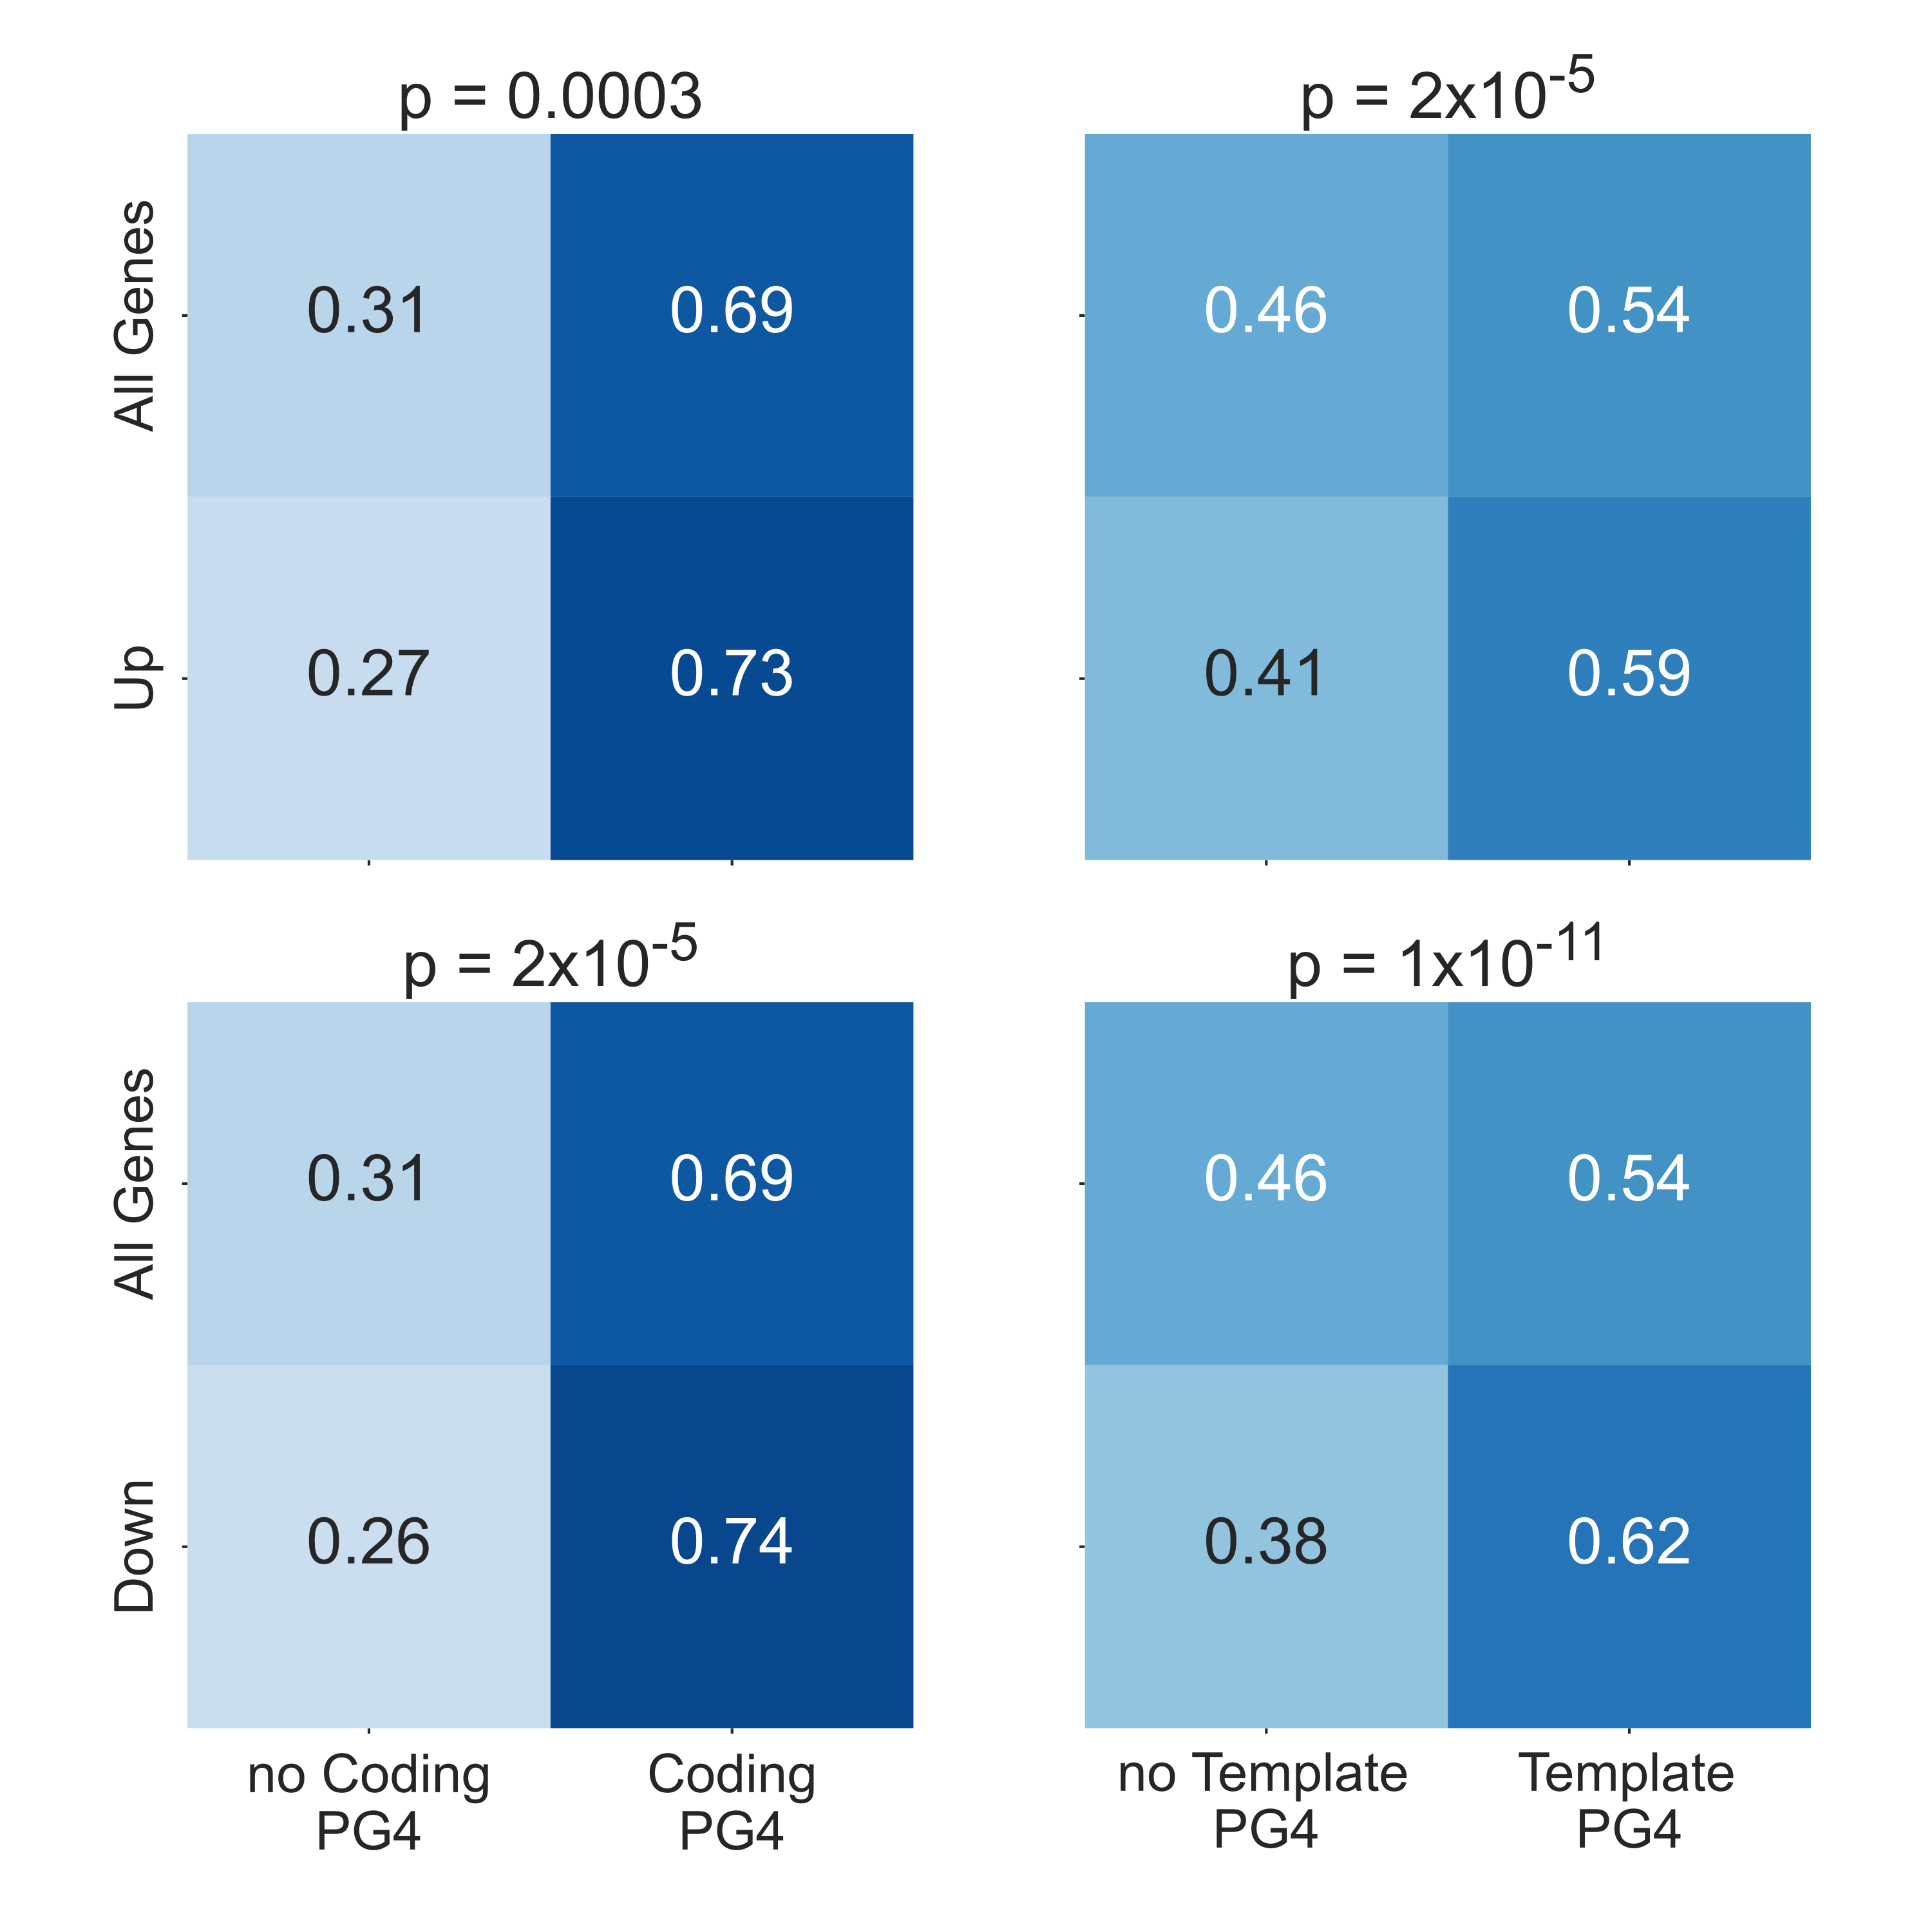
\includegraphics[width=\textwidth,height=562pt,keepaspectratio]{chapter_5/figures/drought_g4_presence_absence_chisquared.png}
\caption[Drought downregulated genes are enriched in PG4s]{\textbf{Drought   downregulated   genes   are   enriched   in   PG4s}   Heatmaps   showing   fractions   of   genes   containing   at   least   one   predicted   G4   in   their   gene   body   for   drought   upregulated   genes   vs   all   genes   (top   row)   and   drought   downregulated   genes   vs   all   genes   (bottom   row)   (For   down   and   upregulated   genes,   FDR   <   0.05   and   absolute   logFC   >   0.5).   PG4   predictions   for   the   coding   strand   are   in   the   left   hand   column   whilst   PG4   predictions   for   template   strand   are   on   the   right.   P   values   for   each   heatmap   are   calculated   using   Chi-squared   tests.   Genes   downregulated   by   drought   stress   show   a   particularly   strong   enrichment   of   PG4s,   and   particularly   on   the   template   strand.   \label{drought_g4_sq}}
\end{figure}

\newpage

\begin{figure}[htbp]
\centering
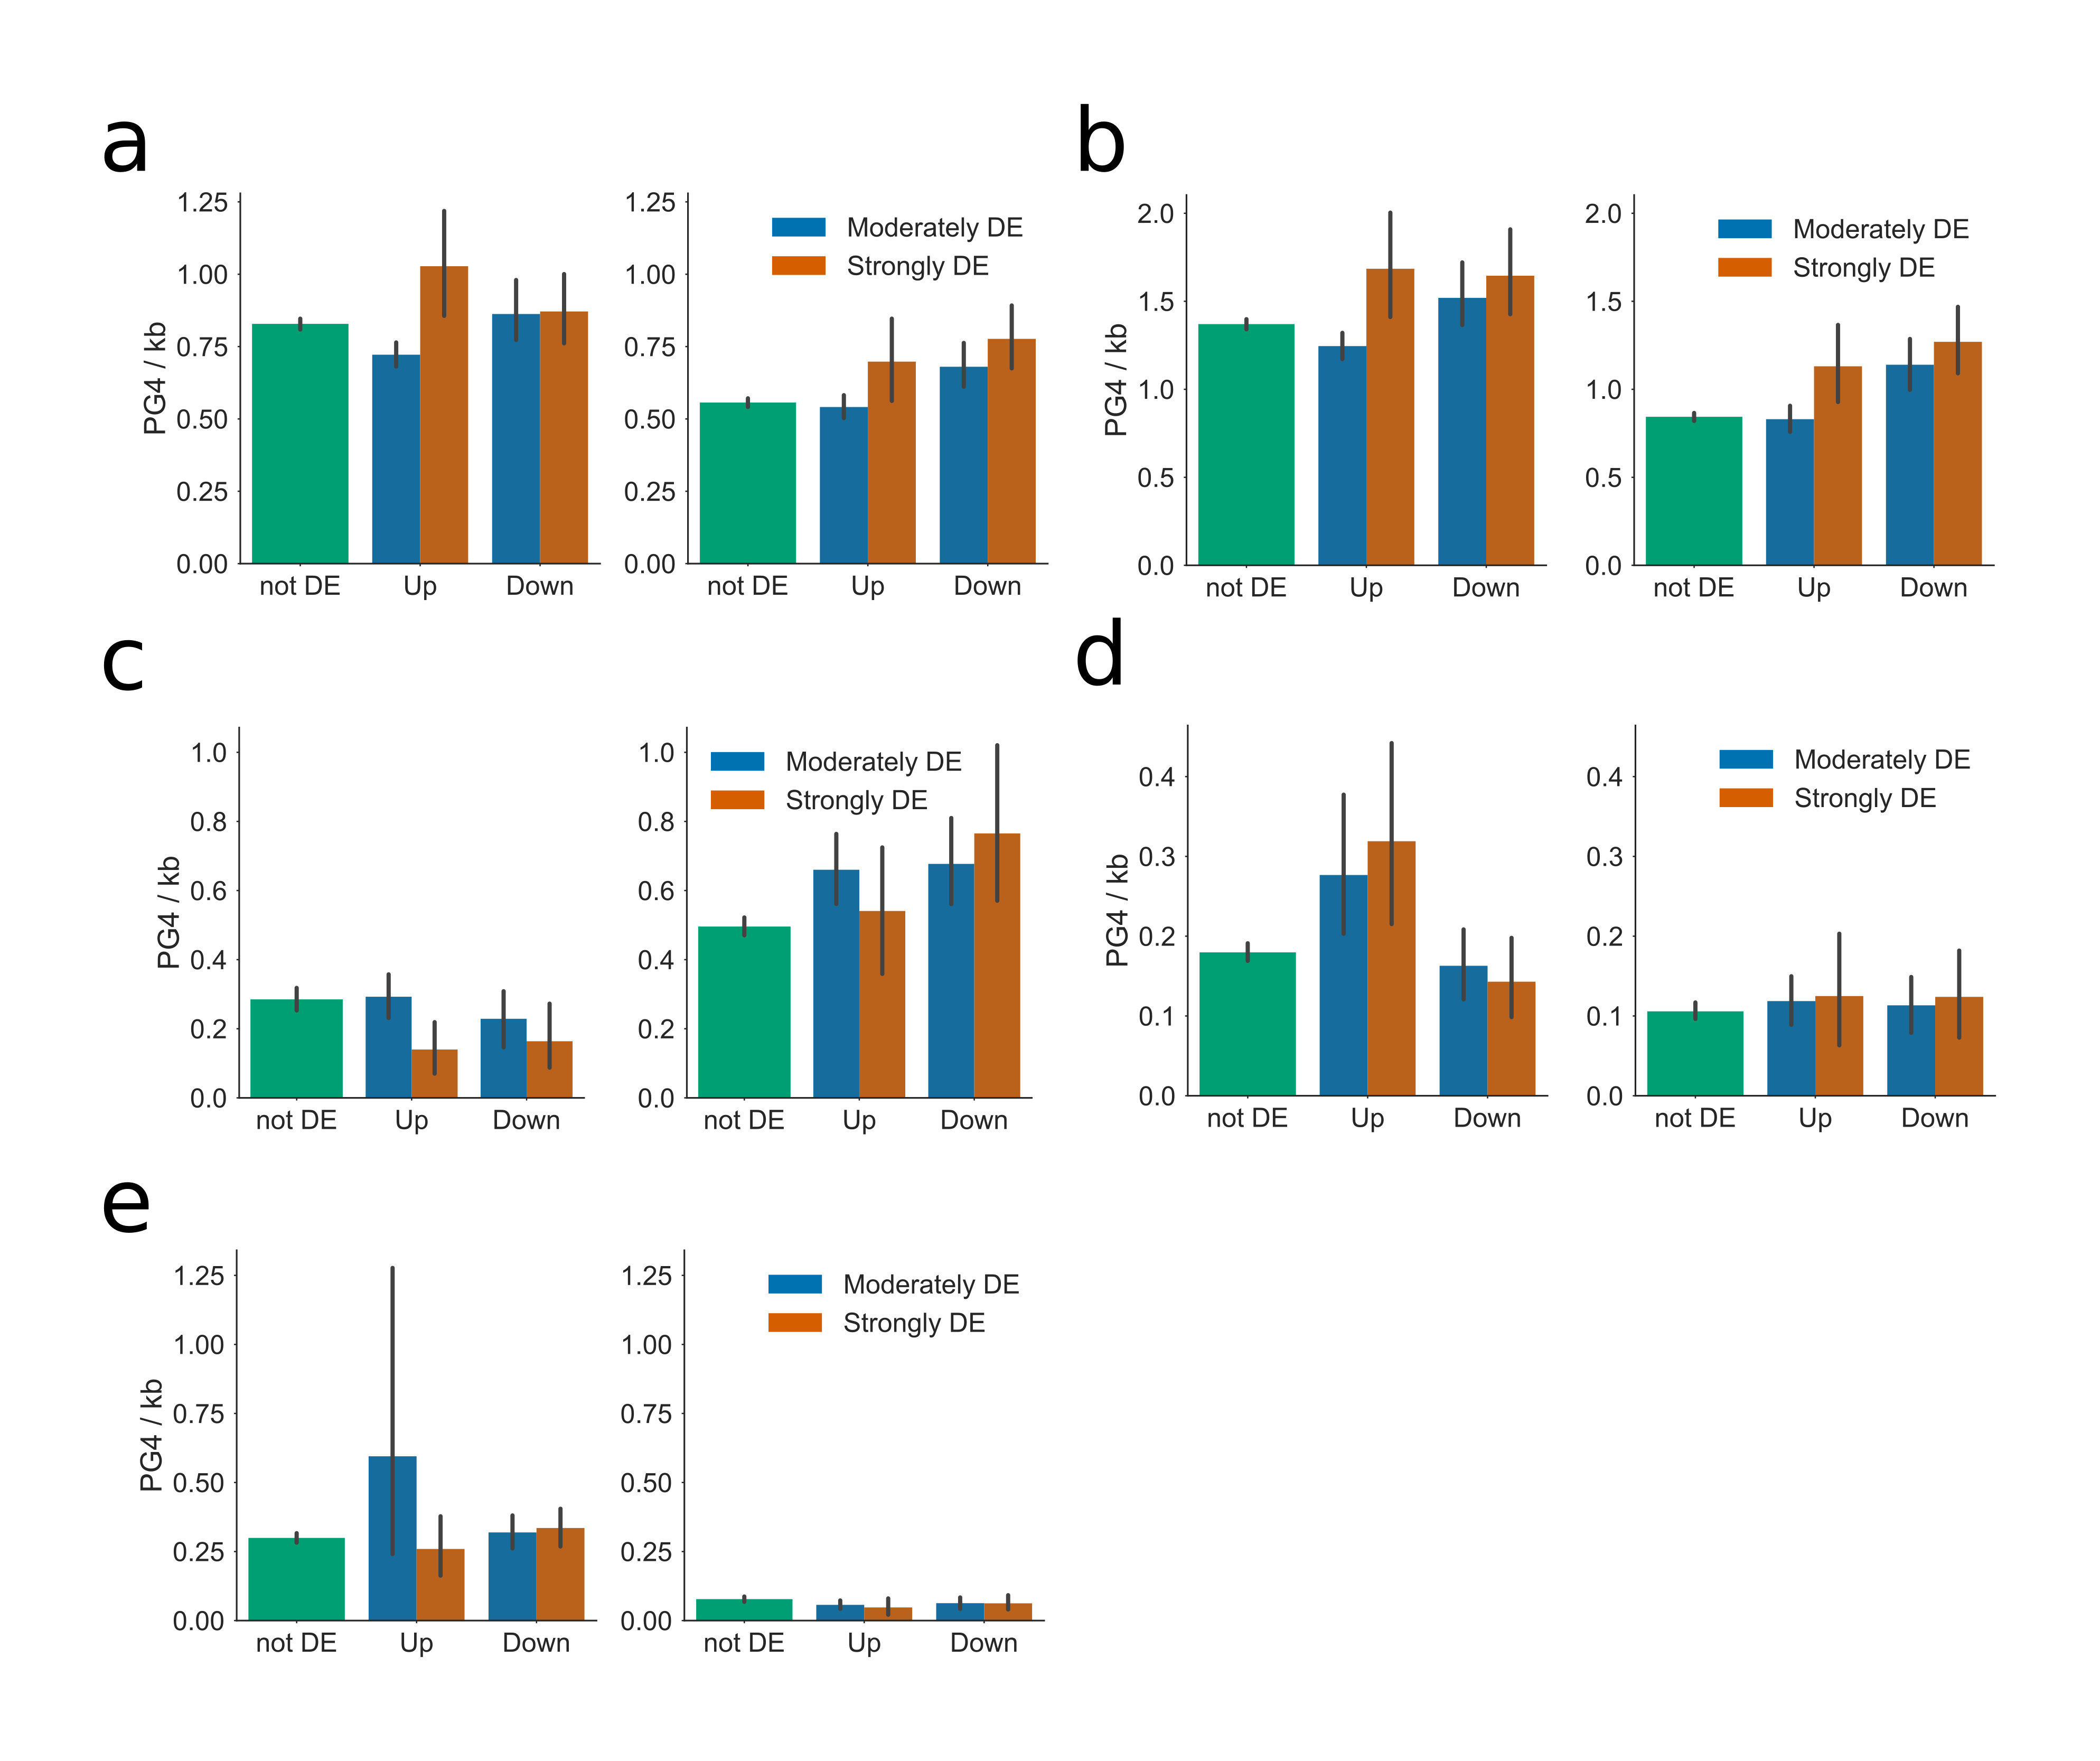
\includegraphics[width=\textwidth,height=562pt,keepaspectratio]{chapter_5/figures/drought_regulated_g4_distribution.png}
\caption[Distribution of PG4s in genes differentially regulated by Drought stress.]{\textbf{Distribution   of   PG4s   in   genes   differentially   regulated   by   Drought   stress.}   Bar   plots   showing   the   average   PG4   densities   of   genes   up   or   downregulated   by   Drought   stress,   for   \textbf{a)}   full   gene   body   (exons   and   introns),   \textbf{b)}   coding   regions,   \textbf{c)}   5’   UTR,   \textbf{d)}   3’   UTR,   and   \textbf{e)}   introns,   respectively.   In   each   figure,   left   and   right   panels   represent   coding   and   template   strand,   respectively.   Genesets   are   separated   into   three   categories   by   strength   of   regulation:   green:   not   differentially   expressed,   blue:   moderately   differentially   expressed   (PPLR   <   0.05,   logFC   >   0.5),   orange:   strongly   differentially   expressed   (PPLR   <   0.05,   logFC   >   1).   Errorbars   are   68\%   confidence   intervals   for   mean   generated   using   1000   bootstrapped   samples.   Genes   which   are   downregulated   by   drought   stress   tend   to   have   higher   PG4   densities   on   the   template   strand   of   coding   regions   and   5’   UTRs.   Genes   which   are   upregulated   by   drought   stress   are   more   likely   to   contain   PG4s   in   their   3’   UTRs.   \label{drought_g4}}
\end{figure}

\newpage

Next we investigated whether there were any similarities in the
expression profiles of NMM treated seedlings and drought stressed
plants. We found a strong overlap between genes moderately downregulated
by NMM and those moderately downregulated by drought stress (p =
1.7e-196) (Fig \ref{nmm_drought}a). Analysis of the PG4 density of these
gene sets and the overlap between them showed that the genes which were
downregulated in both experiments tended to be the most PG4 rich,
particularly in the 5' UTR of the gene (Fig \ref{nmm_drought}b). This
suggests that these genes could indeed be regulated through the same
mechanism of G4 stabilisation.

\newpage

\begin{figure}[htbp]
\centering
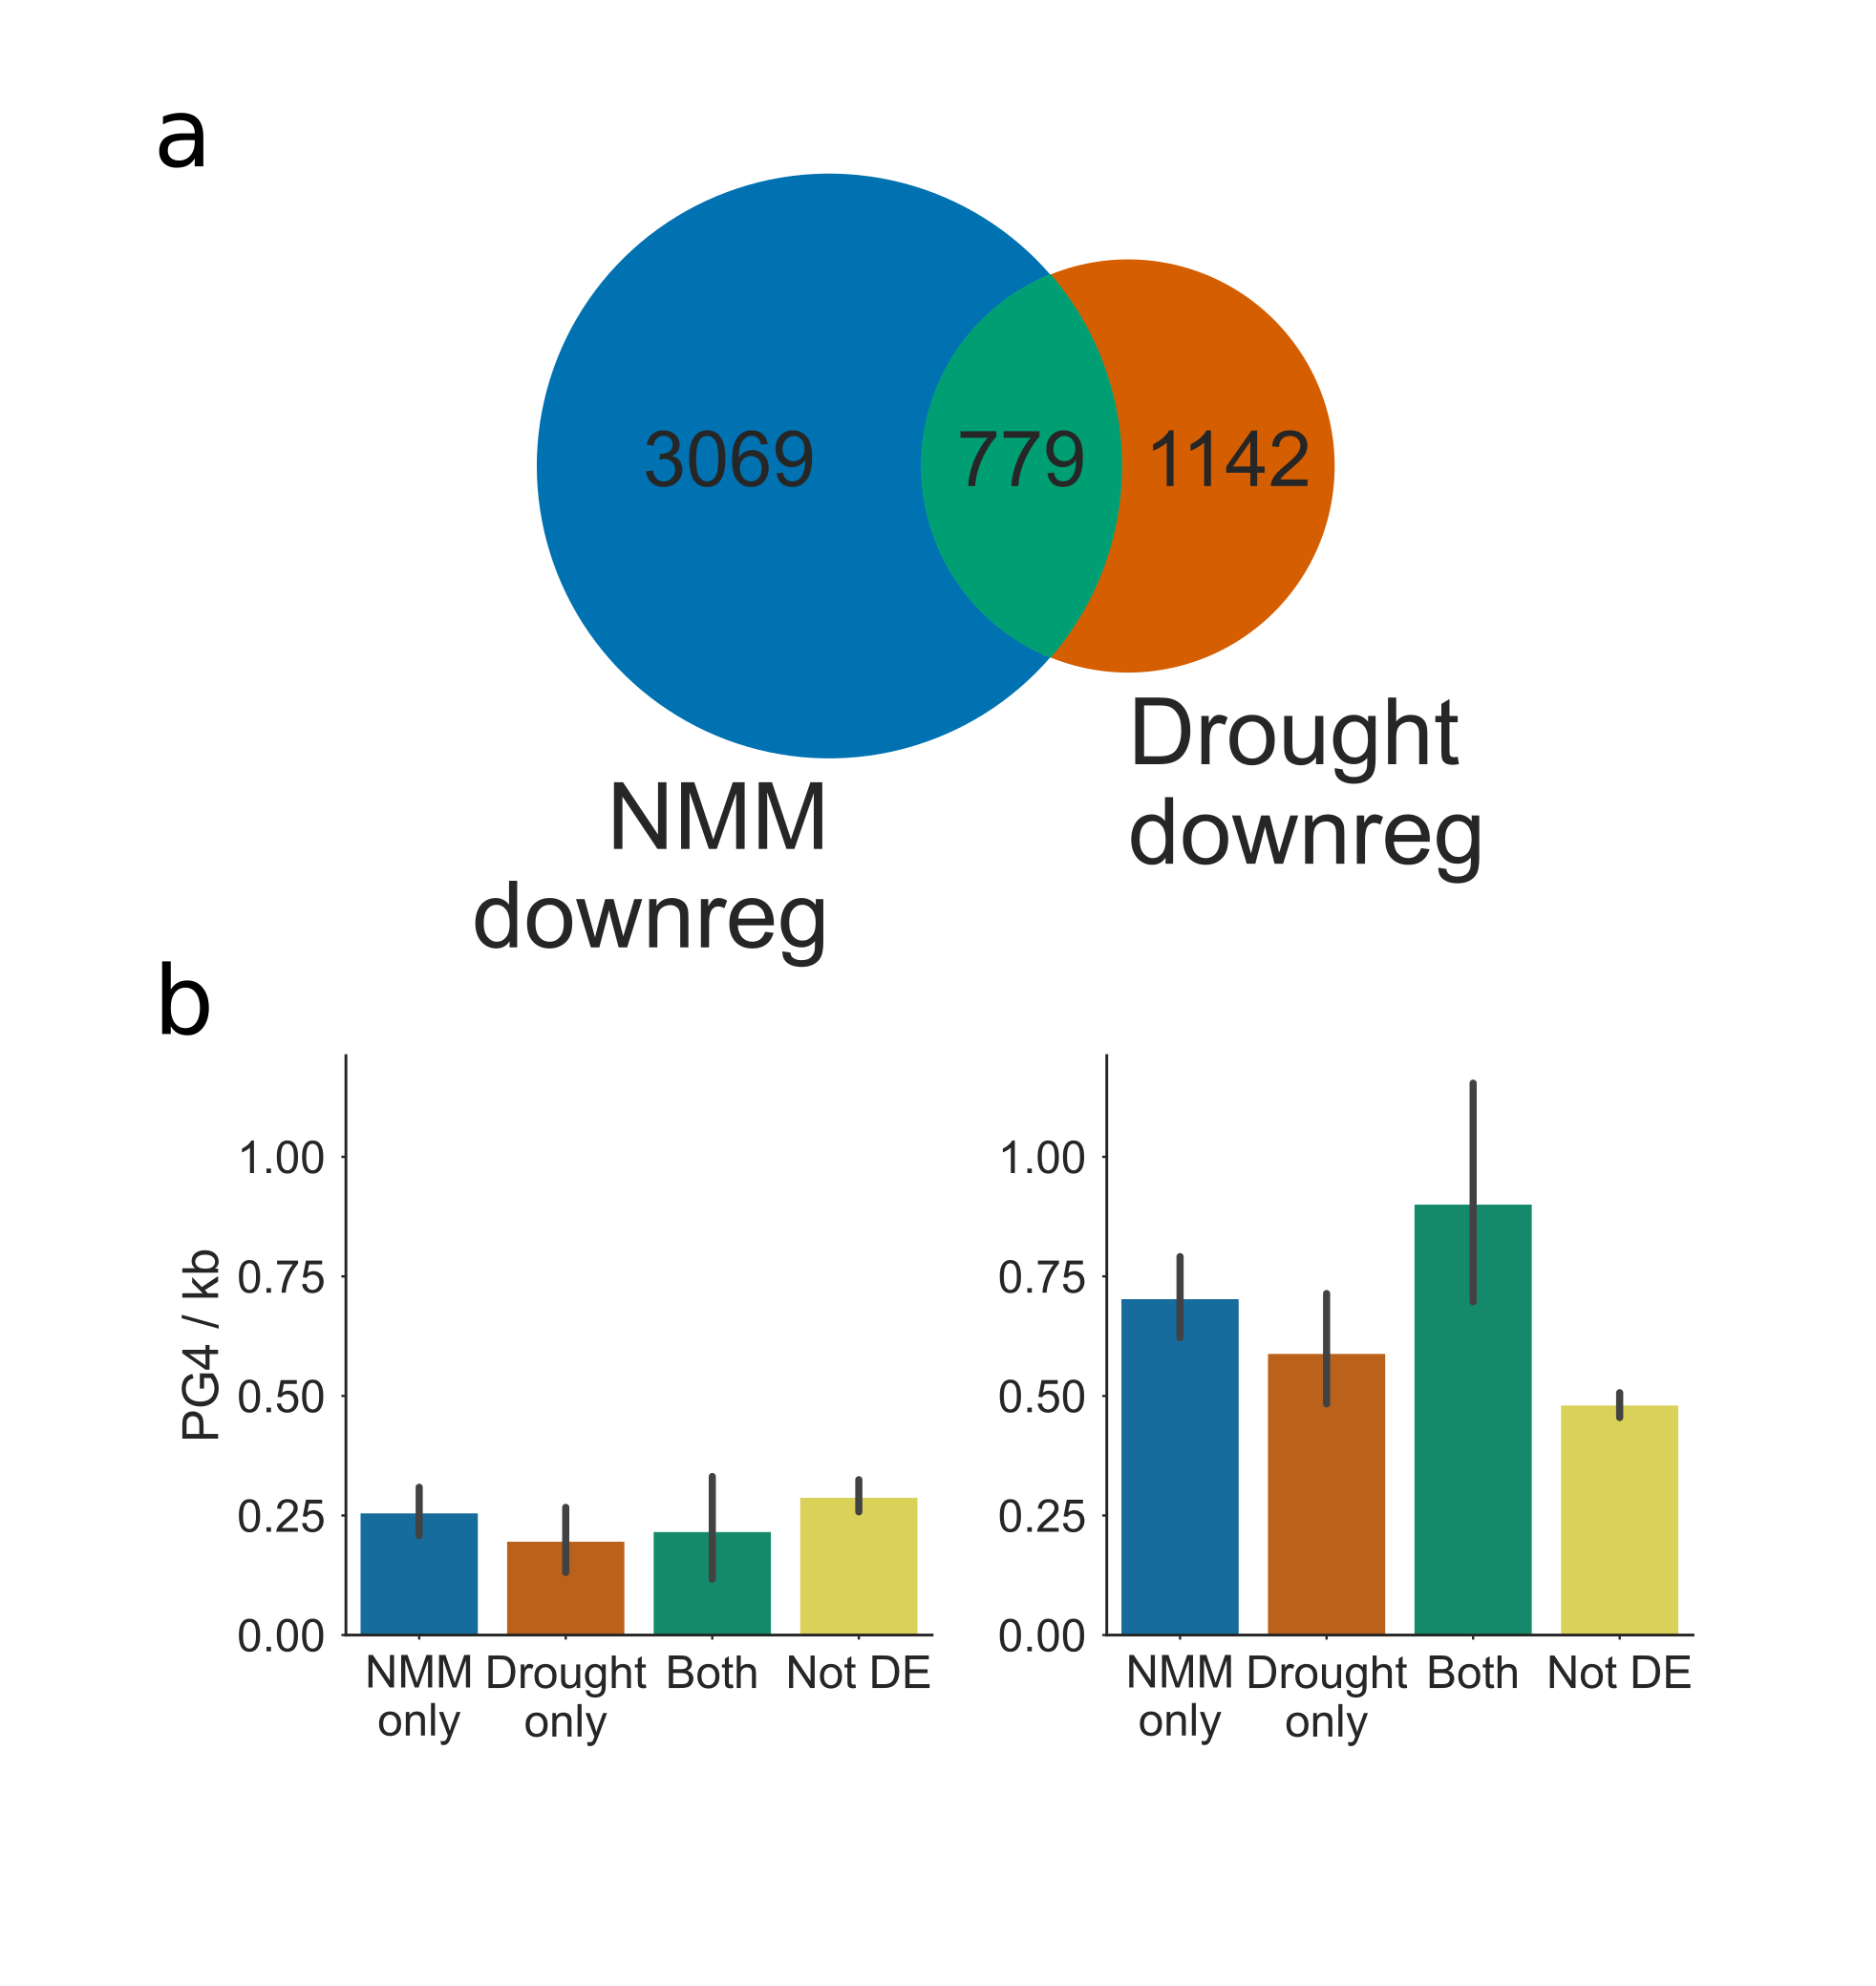
\includegraphics[width=\textwidth,height=562pt,keepaspectratio]{chapter_5/figures/nmm_drought_venn.png}
\caption[Overlap of genes downregulated by NMM with those downregulated by Drought stress.]{\textbf{Overlap   of   genes   downregulated   by   NMM   with   those   downregulated   by   Drought   stress.}   \textbf{a)}   Venn   diagram   reporting   the   overlap   of   genes   downregulated   by   NMM   with   those   downregulated   by   drought   stress.   \textbf{c)}   Bar   plot   showing   the   average   PG4   densities   in   5’   UTRs   of   NMM   and   drought   stress   downregulated   genesets.   Left   and   right   panels   show   densities   on   the   coding   and   template   strands,   respectively.   Both   genesets   show   an   greater   exonic   G4   density   on   the   template   strand   than   genes   not   regulated   by   either   drug,   however   genes   which   are   regulated   by   both   drugs   had   the   greatest   average   PG4   density   in   5’   UTRs.   Bar   colours   match   set   colours   from   Fig   3b.   Errorbars   are   68\%   confidence   intervals   for   mean   generated   using   1000   bootstrapped   samples.   \label{nmm_drought}}
\end{figure}

\newpage

\hypertarget{nmm-affects-gene-expression-in-zea-mays}{%
\subsection{\texorpdfstring{NMM affects gene expression in \emph{Zea
mays}}{NMM affects gene expression in Zea mays}}\label{nmm-affects-gene-expression-in-zea-mays}}

A recently published study by Tokan et al.~provides the first analysis
of differential expression during NMM treatment in a crop plant,
\emph{Zea mays} (Tokan et al., 2018). Their paper focussed on the effect
of NMM on the expression of transposable elements, however, we
reanalysed their data to identify whether protein-coding genes in maize
respond to NMM similarly to Arabidopsis. We found a strong overlap
between genes differentially regulated in Arabidopsis and their
orthologs in maize, in both the up- and downregulated genesets (Fig.
\ref{maize_venn}a and b respectively). Furthermore, we found that maize
genes which were differentially regulated by NMM tended to have greater
two tetrad PG4 densities in their CDSs. Unlike Arabidopsis, however,
this increase in PG4 density was not restricted to the template strand,
and not only in downregulated genes. Genes which are upregulated by NMM
in maize are also more likely to contain CDS PG4s on both the coding and
template strands (Fig \ref{maize_pg4}a). This suggests some other
mechanism of G4 regulation beyond Pol II stalling. Whilst 5' UTRs of
maize genes tend to have high densities of PG4s on the template strand
(Fig \ref{maize_pg4}b, right panel), we did not see a greater level of
PG4s in either up- or downregulated sets. In fact, downregulated genes
appear to have fewer template strand PG4s in the 5'UTR (Fig
\ref{maize_pg4}b, right panel). Interestingly, upregulated genes also
tended to have greater levels of coding and template PG4s in introns
(Fig \ref{maize_pg4}c).

\newpage

\begin{figure}[htbp]
\centering
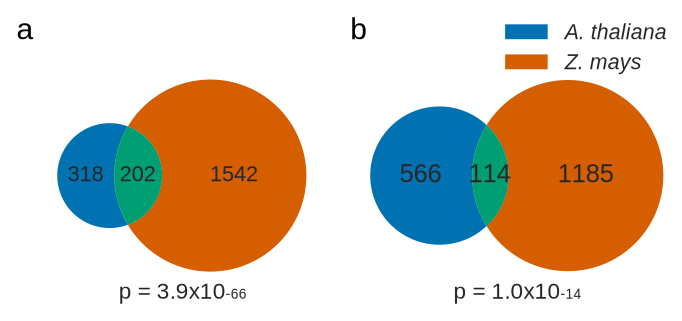
\includegraphics[width=\textwidth,height=562pt,keepaspectratio]{chapter_5/figures/zmays_athaliana_nmm_expression_venn.png}
\caption[NMM expression change of Arabidopsis and \textit{Zea mays} orthologs]{\textbf{NMM   expression   change   of   Arabidopsis   and   \textit{Zea   mays}   orthologs}   Venn   diagrams   showing   the   overlap   between   the   set   of   genes   \textbf{a)}   upregulated   and   \textbf{b)}   downregulated   by   NMM   in   Arabidopsis   and   the   unique   set   of   Arabidopsis   orthologs   for   \textit{Z.   mays}   genes   regulated   by   NMM.   P   values   were   calculated   by   hypergeometric   test   compared   to   the   unique   set   of   \textit{Arabidopsis}   genes   with   at   least   one   \textit{Z.   mays}   ortholog.   \label{maize_venn}}
\end{figure}

\newpage

\begin{figure}[htbp]
\centering
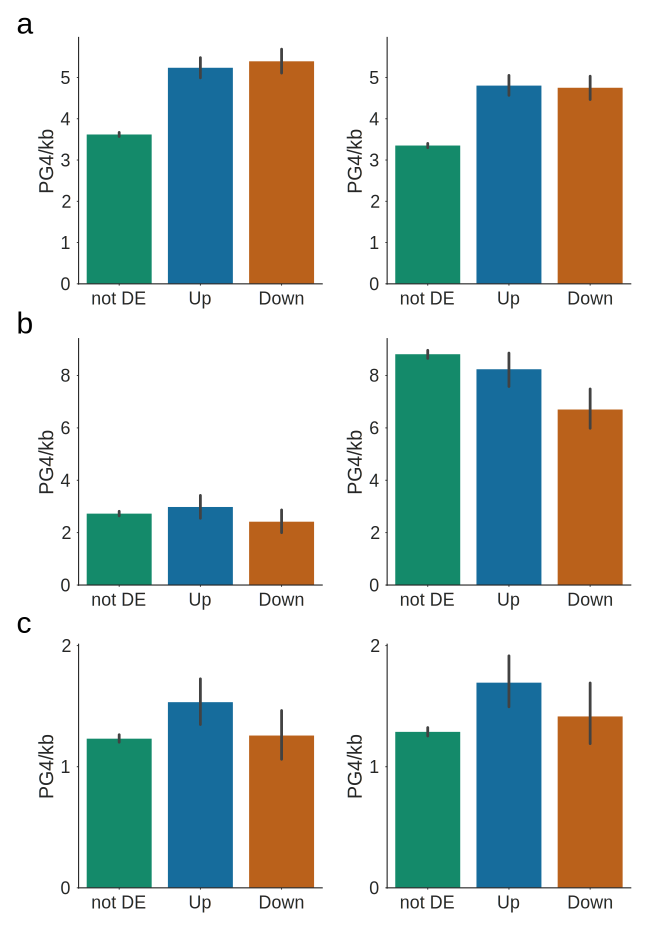
\includegraphics[width=\textwidth,height=562pt,keepaspectratio]{chapter_5/figures/zmays_nmm_g4_distribution.png}
\caption[Distribution of Two tetrad PG4s in \textit{Z. mays} genes regulated by NMM]{\textbf{Distribution   of   Two   tetrad   PG4s   in   \textit{Z.   mays}   genes   regulated   by   NMM}   Bar   plots   showing   the   average   PG4   densities   of   \textit{Z.   mays}   genes   up   or   downregulated   by   NMM,   for   \textbf{a)}   CDSs,   \textbf{b)}   5’   UTRs   and   \textbf{c)}   introns,   respectively.   In   each   figure,   left   and   right   panels   represent   coding   and   template   strand,   respectively.   Errorbars   are   68\%   confidence   intervals   for   bootstrapped   means.   \label{maize_pg4}}
\end{figure}

\newpage

\hypertarget{discussion-1}{%
\section{Discussion}\label{discussion-1}}

We have conducted the first in detail analysis of the effects of G4
stabilisation in the higher plant, \emph{Arabidopsis thaliana}. To
determine how gene expression is altered by G4 stabilisation, we carried
out a microarray analysis of plants treated with the G4 binding drug,
NMM. NMM treatment had very strong effects on gene expression,
particularly in genes which contained large numbers of parallel two
tetrad G4s in the transcribed gene body. Moderately downregulated genes
had large numbers of G4s in their 5' UTRs, whilst very strongly
downregulated genes contained large numbers of G4s throughout the exonic
regions of the gene. This is contrary to evidence from human systems
which has suggested G4s influence transcription most when located in the
promoter region. Furthermore, we find that the effect on gene expression
is entirely strand dependent: only template stranded G4s strongly affect
expression. Many previous studies have suggested that two tetrad G4s are
not biologically relevant due to their relative instability compared to
three tetrad G4s. The majority of these studies have been focussed upon
their role in human biology. However, several other studies have shown
that two tetrad G4s are stable \emph{in vitro} and at physiological
temperatures. In organisms that exist at lower temperatures it is
entirely credible that two tetrad G4s may play a role. Indeed, here we
find that the strongest effect of NMM treatment is on genes predicted to
form only two tetrad G4s.

Since the effect of NMM on gene expression mainly appears to be confined
to genes with template stranded G4s, G4s will not be present in the mRNA
of downregulated genes. Any direct binding of NMM to G4s must therefore
occur in the DNA. The most likely explanation for a template stranded
effect is that stabilised G4s interact with the elongating Pol II, which
uses the non-coding strand of genes as a template for RNA
polymerisation. Since G4s have previously been shown to cause polymerase
stalling in vitro, we investigated the Pol II occupancy profiles of G4
containing genes. This data showed that G4 containing genes had higher
Pol II density at the TSS proximal end of the gene, and lower density at
the TTS. An increase in Pol II occupancy could be explained by one of
two factors: more Pol II molecules binding and initiating transcription;
or a reduction in Pol II speed. We suggest that G4s in the template
strand block the elongation process and cause Pol II to slow down,
resulting in a higher Pol II occupancy upstream of the G4 dense region.
The Pol II data analysed is captured in the absence of any G4
stabilising drugs, indicating that G4 dependent Pol II slowing is a
commonly occurring phenomenon. We hypothesise that two tetrad G4s form
naturally in genes, causing Pol II slowing, but still creating full
length products. Changes in Pol II speed may have consequential effects
for co-transcriptional processes such as mRNA splicing. In some cases
blockages may cause premature termination, resulting in truncated
products. Analysis of the ratio of GRO/RNAseq read counts suggests that
G4 dense genes do indeed produce slightly more unstable products than
genes containing no G4s. In the presence of NMM, however, stabilised G4s
are likely to become too difficult for the transcription complex to
unwind, and cause greater levels of premature termination, the products
of which are presumably degraded. The result of this is the dramatic
downregulation seen in the microarray.

Previous studies of PG4 localisation in Arabidopsis have highlighted a
greater number of two tetrad PG4s in genes annotated as responsive to
drought than expected given the distribution across all genes (Mullen et
al., 2010, 2012). Since intracellular potassium levels are increased
during drought stress, it is possible that the stability of G4s could be
increased. To investigate this potential G4 dependent regulatory
mechanism, we analysed microarray data from drought stressed plants. We
found that genes which are downregulated by drought stress contained
more PG4s in the template strand, particularly in 5' UTRs and to a
lesser extent in coding regions. This result matched closely to the
enrichment of G4s in genes downregulated by NMM. Indeed, when we studied
the overlap between drought stress downregulated genes and NMM
downregulated genes, we found a strong overlap. Furthermore, the genes
which were downregulated in both conditions were those which had the
greatest PG4 density in their 5' UTRs. We suggest that during drought
stress G4s in these genes form more strongly, causing blockages that
pause Pol II, downregulating the expression of the gene. Finally, we
found that genes upregulated by drought stress tended to contain higher
levels of G4s in their 3' UTRs. This effect was not replicated by NMM
treatment, suggesting an alternative mechanism of action. Since the 3'
UTR is known to be an important regulator of mRNA stability and
translation, we speculate these G4s form more strongly in the mRNA
during drought stress and recruit some G4 binding factor which could
enhance the stability of the mRNA.

\newpage

\hypertarget{effect-of-g-quadruplexes-on-expression-and-splicing-of-the-extensin-gene-family}{%
\chapter{Effect of G-Quadruplexes on expression and splicing of the
Extensin gene
family}\label{effect-of-g-quadruplexes-on-expression-and-splicing-of-the-extensin-gene-family}}

\label{chap:extensins}

\hypertarget{introduction-4}{%
\section{Introduction}\label{introduction-4}}

\label{sec:extensin_intro}

It is well characterised that G4s have the ability to stall polymerases,
including both DNA and RNA polymerases (Han et al., 1999; Siddiqui-Jain
et al., 2002; Cogoi and Xodo, 2006; Dexheimer et al., 2006; Chambers et
al., 2015; Kwok et al., 2016). This has been demonstrated through
\emph{in vitro} Polymerase stop assays as well as by identifying
transcriptionally dependent DNA breaks during G4 ligand treatment
(Rodriguez et al., 2012). Furthermore a number of helicases which are
associated with the transcription initiation factor (TFIIH) and
elongation, including BLM, WRN and XPD, have been shown to
preferentially bind and unwind G4 DNA \emph{in vitro} (Sun et al., 1998;
Mohaghegh et al., 2001; Gray et al., 2014). XPD has also been associated
with human TSSs containing PG4s by ChIP-seq (Gray et al., 2014). This
evidence points to an effect of G4s on elongation by Pol II. We showed
in \autoref{chap:global_nmm} that PG4 dense genes appeared to have
slower elongation of Pol II and hence increased Pol II occupancy at the
start of the gene. This reduction in Pol II speed may have knock-on
effects on co-transcriptional modifications, such as splicing of mRNA.
Furthermore, if G4 stabilisation can be regulated, this could constitute
a new mechanism for the regulation of splicing.

It has been estimated that around 80\% of all splicing occurs
co-transcriptionally in higher eukaryotes (Carrillo Oesterreich et al.,
2010; Ameur et al., 2011; Khodor et al., 2011; Girard et al., 2012;
Tilgner et al., 2012; Windhager et al., 2012). This is likely due to the
coupling of splicing to export and quality control mechanisms (Reed and
Hurt, 2002; Stäßer et al., 2002; Fan et al., 2017). How splicing occurs
is highly dependent on Pol II speed, since changes in speed can alter
how strong and weak splice junctions compete for assembly of
spliceosomes (Mata et al., 2010; Jonkers and Lis, 2015). The classic
mechanism involving differential acceptor site usage is shown in (Fig
\ref{speed_splice}a). When Pol II is elongating at high speed, acceptor
sites which are more strongly canonical but further from the donor in
sequence space are favoured. This is because on average, the greater
strength of the canonical junctions outweigh the extra time that weaker
junctions which are closer in sequence space have to be spliced. When
Pol II elongates more slowly, however, weak acceptor sites which are
more proximal may have much more time to be utilised before stronger
distal acceptors are transcribed into the nascent RNA. This tips the
balance towards utilisation of weak splice junctions, and can result in
alternative splicing (AS) (Mata et al., 2010; Jonkers and Lis, 2015).

\newpage

\begin{figure}[htbp]
\centering
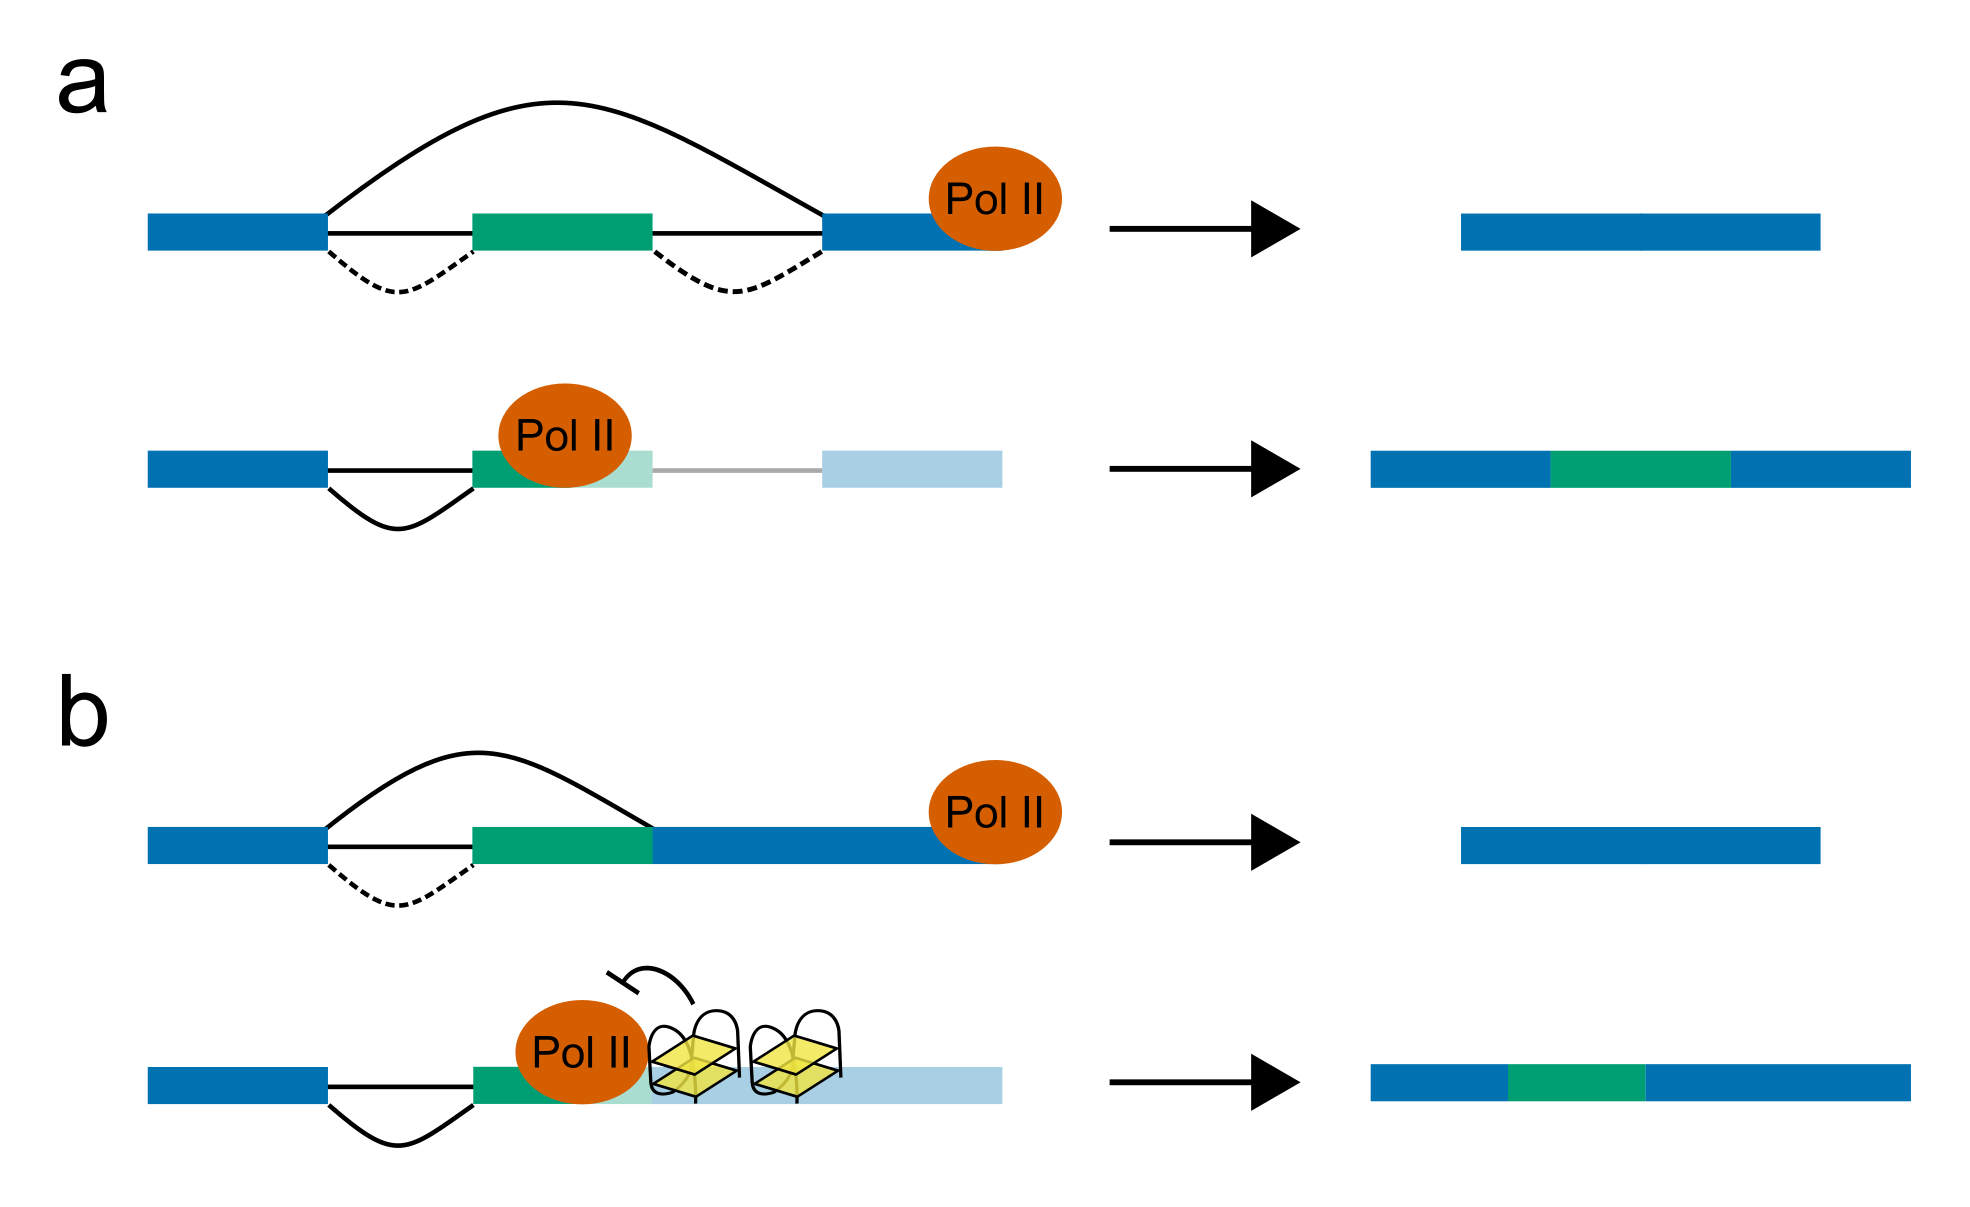
\includegraphics[width=\textwidth,height=562pt,keepaspectratio]{chapter_6/figures/polii_speed_splicing.png}
\caption[Pol II elongation speed affects co-transcriptional splicing]{\textbf{Pol   II   elongation   speed   affects   co-transcriptional   splicing}   \textbf{a)}   Mechanism   for   effect   of   Pol   II   speed   on   co-transcriptional   splicing:   when   elongation   occurs   rapidly   (first   row),   the   more   canonical   but   distal   acceptor   site   is   used,   resulting   in   the   exclusion   of   the   alternate   exon   (shown   in   green).   When   Pol   II   elongates   more   slowly   (second   row),   there   is   more   time   for   the   weaker   proximal   site   to   be   utilised,   resulting   in   the   inclusion   of   the   alternate   exon.   \textbf{b)}   Example   mechanism   for   how   G4s   could   affect   splicing.   When   G4s   are   not   present   (top   row),   the   constitutive   splice   acceptor   is   used   and   the   green   exonic   chunk   is   excluded.   When   G4s   are   formed   in   the   template   strand   of   the   DNA   (second   row),   these   slow   down   Pol   II   elongation,   allowing   the   weaker   proximal   splice   junction   to   be   utilised,   and   including   the   alternate   exon   chunk.   \label{speed_splice}}
\end{figure}

\newpage

In mammalian systems, the most common form of AS appears to be exon
skipping (\textgreater{}40\% of AS exons). Intron retention occurs at
low rates in human transcriptomes (10\% of AS exons), whilst in
Arabidopsis, it is much more common (30-35\% of AS exons)
({\textbf{???}}; Kim et al., 2007). Marquez et al.~recently identified a
novel form of intron retention, called the exitron, in human and
Arabidopsis transcriptomes (Marquez et al., 2012, 2015). Exitrons are
intronice regions which more closely resemble exonic sequence in their
GC content, are multiples of three in length and do not contain in-frame
stop codons ({\textbf{???}}; Marquez et al., 2012, 2015). These occur in
coding regions of the mRNA, contributing to the protein sequence when
spliced in, and causing truncations of the protein sequence when spliced
out. Marquez et al.~found exitrons to be relatively common in long exons
of Arabidopsis genes (Marquez et al., 2012, 2015). The study also found
evidence of protein products from these exitrons, indicating that unlike
intron retention events, which are thought to be regulatory or caused by
splicing errors, exitronic transcripts are functional at the protein
level.

Here we identify a novel family of PG4 rich genes, which are
downregulated by NMM, and appear to be heavily exitronically spliced. We
characterise this splicing and identify whether it can be altered
through G4 stabilisation by NMM.

\newpage

\hypertarget{methods-1}{%
\section{Methods}\label{methods-1}}

\label{sec:extensin_methods}

\hypertarget{plant-growth-conditions-and-drug-treatments}{%
\subsection{Plant growth conditions and drug
treatments}\label{plant-growth-conditions-and-drug-treatments}}

All experiments used Arabidopsis thaliana Columbia (Col-0) ecotype and
all mutant plants used were of Col-0 background. For all experiments
seeds were surface sterilised, stratified for 2-3 days at 4°C then sown
on vertical plates containing Murashige \& Skoog (MS) agar with 1\%
sucrose and 0.8\% agar and transferred to growth cabinets at constant
light at 23°C (growth time refers to the time after transfer to growth
cabinet). Seedlings used for qPCR and RNAseq were grown for 7 days on MS
plates, treated for 6 hours by flooding the plate with MS liquid media
containing the drug after which roots and shoots are harvested
separately. Drugs used were N-Methyl Mesoporphyrin (Frontier Scientific,
NMM580), Berberine (Sigma B3251) and Cyclohexamide (Sigma C7698). For
combined Cyclohexamide and NMM treatment, plants were pretreated for 2
hours with Cyclohexamide before adding NMM and treating for a further 6
hours.

\hypertarget{rna-extraction-for-qpcr-and-rnaseq}{%
\subsection{RNA extraction for qPCR and
RNAseq}\label{rna-extraction-for-qpcr-and-rnaseq}}

Total nucleic acid isolation protocol was carried out by
phenol-chloroform extraction as described by White and Kaper (White and
Kaper, 1989). The resulting pellets were resuspended in sterile water
and stored at -80C. The RNA concentration and quality was checked using
the NanoDrop 1000 Spectrophotometer (ThermoScientific). DNA
contamination was removed using DNase I (Sigma AMPD1).

\hypertarget{rnaseq-analysis}{%
\subsection{RNAseq analysis}\label{rnaseq-analysis}}

RNA was sent to Sheffield Children's Hospital Genomics Facility for
library preparation and sequencing. Polyadenylated RNA was enriched
using NEBNext Poly(A) mRNA Magnetic Isolation, and libraries were
produced using the NEBNext Ultra II Directional RNA kit for Illumina.
The chemical fragmentation step was adjusted to increase estimated
insert size to the 400-450bp range. Paired end sequencing was conducted
across two lanes of an Illumina HiSeq 2500 in rapid run mode, with 220bp
read length. The run returned 157 million pass filter reads in lane 1,
and 154 million in lane 2. Initial read preprocessing and adaptor
trimming was conducted by the Genomics Facility.

Read quality was assessed locally using \texttt{FastQC} (Andrews, 2010).
Differential expression analysis was conducted by using \texttt{salmon}
pseudoalignment (Patro et al., 2017) to estimate transcript abundance
against Araport11 cDNA and ncRNA (Cheng et al., 2017). Mean insert size
for each sample was assessed to be in the 400-500bp range. Gene level
abundance was then aggregated from this using \texttt{tximport} (Soneson
et al., 2018) and differential expression testing was conducted using
\texttt{edgeR} linear modelling (Robinson et al., 2009; McCarthy et al.,
2012). Normalised log2 counts per million (CPM) were calculated and used
for plotting. P values were adjusted using the Benjamini Hochberg
multiple testing correction. Barplots of NMM and DMSO expression were
produced using \texttt{seaborn} (Waskom et al., 2014).

Spliced reads were mapped to the TAIR10 genome (The Arabidopsis Genome
Initiative, 2000) using \texttt{STAR} {[}Dobin2013{]}. The parameters
for spliced mapping were adjusted to increase precision. A minimum of
8bp overhang was used for unannotated splice junctions, and 5bp for
annotated splice junctions, following ENCODE guidelines (ENCODE, 2016).
Minimum intron size was set to 60bp and maximum intron size to 10000bp.
Output BAM files were sorted and indexed using \texttt{samtools} (Li et
al., 2009).

\hypertarget{gene-ontology-analysis}{%
\subsection{Gene Ontology analysis}\label{gene-ontology-analysis}}

For PG4 enrichment Ontology analysis, two tetrad Quadparser PG4s were
predicted in the TAIR10 genome using \texttt{g4predict}. The number of
PG4s overlapping each strand of the flattened exon models for each gene
in Araport11 (Cheng et al., 2017) was calculated using
\texttt{bedtools\ intersect} (Quinlan and Hall, 2010). To calculate
enrichment, a permutation test experiment was conducted, where each gene
was assigned a weighting proportional to the total length of its exonic
sequence. PG4s were then shuffled randomly amongst all genes. For each
Ontology group, the number of PG4s observed in genes of that group was
compared to the expected numbers if PG4s were distributed randomly
across the transcriptome. 10000 permutations were used for testing, and
two tailed P values were calculated as
\(max(min(\frac{\sum_{i=0}^nexp_i < obs}{n}, \frac{\sum_{i=0}^nexp_i > obs}{n}), \frac{1}{n})\),
where \(n\) is the total number of permutations and \(exp_i\) is the
expected value from the \(i\)th permutation. P values were adjusted
using the Benjamini Hochberg multiple testing correction.

For Gene Ontology analysis of differentially expressed genes,
\texttt{GOseq} was used (Young et al., 2010). Up and downregulated
genesets were produced using a log2 fold change threshold of 1 and an
FDR of 0.05. Weighting factors used were the median transcript length
for each gene. P values for enrichment were produced by \texttt{GOseq}
using the Wallenius approximation method and were corrected for multiple
testing using the Benjamini Hochberg method.

Tables of enriched GO terms were generated using \texttt{pandas}
(Mckinney, 2011) and formatted with \texttt{inkscape}.

\hypertarget{extensin-gene-family-total-pg4-estimation}{%
\subsection{Extensin gene family total PG4
estimation}\label{extensin-gene-family-total-pg4-estimation}}

For estimated PG4 numbers in the table in Fig \ref{ext_table}, PG4s were
predicted using three different methods. All instances of the
dinucleotide \texttt{GG} were identified in each Extensin gene, and then
a graph was built where each \texttt{GG} was a node and nodes were
connected by an edge if dinucleotides were less than 7bp apart from each
other. The number of overlapping PG4 conformations was then calculated
as the number of subgraphs in the graph with exactly four members,
whilst the number of merged PG4s was calculated as the number of
unconnected subgraphs with four or more members. To identify the number
of non-overlapping PG4s, a dynamic programming method was used.
Overlapping PG4s were grouped and scored by inverse length, then
filtered for the maximum number of high scoring, non-overlapping PG4s.

\hypertarget{quantitative-pcr-experiments}{%
\subsection{Quantitative PCR
experiments}\label{quantitative-pcr-experiments}}

Total RNA was reverse transcribed into cDNA using the High Capacity cDNA
Reverse Transcription Kit with a PolyT primer (Invitrogen Cat.
No.~4368813). qPCR was carried out using SYBR® Green JumpStart™ Taq
ReadyMix™ (Sigma-Aldrich Cat. No.~S4438) using the Mx3000P qPCR System
(Agilent Technologies). Thermal cycling conditions consist of a
denaturation step at 94 °C for 2 minutes, 40 cycles of 15-second
denaturation at 94 °C and 1-minute extension at 60 °C, then a final
dissociation step of 2 minutes at 94°C, 1 minute at 60 °C and 2 minutes
at 94 °C.

\hypertarget{analysis-of-public-rnaseq-data}{%
\subsection{Analysis of public RNAseq
data}\label{analysis-of-public-rnaseq-data}}

Root RNAseq from PRJNA323955 (Li et al., 2016) was downloaded in FASTQ
format from ENA. Quality assessment was performed with \texttt{FastQC}
(Andrews, 2010) and \texttt{fastq-screen} (Wingett, 2011), and adapter
contamination was removed using \texttt{Cutadapt} (Martin, 2011). The
data was mapped using \texttt{STAR} (Dobin et al., 2013) with default
settings, except than max intron length was set to 10000bp. Output BAM
files were sorted and indexed using \texttt{samtools} (Li et al., 2009).

Normalised gene expression estimates were generated using
\texttt{featureCounts} (Liao et al., 2013) to get raw counts of
alignments overlapping each gene in Araport11 (Cheng et al., 2017), and
\texttt{edgeR} (Robinson et al., 2009; McCarthy et al., 2012) to perform
estimation of log2 counts per million.

\hypertarget{splice-junction-analyses}{%
\subsection{Splice junction analyses}\label{splice-junction-analyses}}

Splice junction sites were extracted from aligned reads using
\texttt{pysam} (Heger et al., 2014). For all analyses, reads were
filtered to produce a set of unique donor/acceptor site pairs. Scatter
plots of spliced read percentages and frequency plots of in frame
exitrons were produced using \texttt{matplotlib} and \texttt{seaborn}
(Hunter, 2007; Waskom et al., 2014).

\hypertarget{sequence-logo-generation}{%
\subsection{Sequence logo generation}\label{sequence-logo-generation}}

Consensus sequence logos were generated using an in-house Python module
\texttt{matplotlib\_logo}. Unique splice junction pairs from spliced
reads were identified, and the corresponding sequence information (8bp
up and downstream of donor and acceptor) was extracted from the TAIR10
genome (The Arabidopsis Genome Initiative, 2000) using \texttt{pysam}
(Heger et al., 2014). Position frequency matrices were generated from
these sequences, and entropy score in bits was calculated and plotted.

\hypertarget{rnaseq-read-simulation-and-bootstrapping-experiment}{%
\subsection{RNAseq read simulation and bootstrapping
experiment}\label{rnaseq-read-simulation-and-bootstrapping-experiment}}

For RNAseq read simulation, read counts generated using
\texttt{featureCounts} (Liao et al., 2013) for each file in the Li et
al.~2016 dataset were used to inform a \texttt{polyester} (Frazee et
al., 2015) simulation of Illumina 125bp paired end reads, using the
Araport11 annotation (Cheng et al., 2017). Fragment length was simulated
using a normal distribution with mean 250bp and standard deviation of
25bp. Error rate was simulated at a uniform 0.5\% across samples, reads,
and nucleotides.

For the bootstrapping experiment, one or more pairs of real and
simulated samples were randomly sampled from the dataset and unique
splice donor/acceptor pairs in EXT9 were identified. Only splice sites
from primary alignments, with overhangs greater than 20bp, and with more
than 2 supporting reads were kept. For each splice site, the exonic
overhang sequence 20bp upstream of the donor site and 20bp downstream of
the acceptor site were extracted from the read and concatenated. Any
splice site whose concatenated sequence was present as a contiguous kmer
in the reference EXT9 sequence was assumed to be a mapping error and
filtered out. Finally, splice sites were deduplicated by directional
clustering of sequences with edit distance of one or less using
\texttt{umi\_tools} directional clusterer (Smith et al., 2017). 500
iterations were used for bootstrapping. 67\% confidence intervals were
produced and plotted using \texttt{seaborn} (Waskom et al., 2014).

\hypertarget{mappability-analyses}{%
\subsection{Mappability analyses}\label{mappability-analyses}}

Mappability scores were generated for the TAIR10 genome using
\texttt{gem-mappability} (Derrien et al., 2012) with a kmer size of
75bp, and converted to \texttt{BigWig} format using \texttt{gem-2-wig}
and \texttt{wigToBigWig} (Kent et al., 2010). Minimum mappability scores
for each Extensin gene were extracted using \texttt{pyBigWig} (Ryan et
al., 2018) and plotted against spliced fraction using
\texttt{matplotlib} (Hunter, 2007).

\hypertarget{sanger-sequencing-analysis}{%
\subsection{Sanger sequencing
analysis}\label{sanger-sequencing-analysis}}

For Sanger sequencing, cDNA was produced using the Invitrogen High
Capacity cDNA Reverse Transcription Kit with a PolyT primer. Gene
specific primers were used to amplify transcripts of interest by PCR.
Products were then cloned using the Thermo Scientific CloneJET PCR
cloning kit, and transformed into DH5alpha competent cells. Colonies
were grown overnight on ampicillin and tested by colony PCR. Picked
colonies were then grown up for a further 24 hours in liquid media
before miniprepping with Qiagen QIAprep Spin Miniprep Kit. Plasmids were
sent, with pJet1.2 forward and reverse sequencing primers, for Sanger
sequencing at the Sheffield Hallamshire Hospital Core Genomics Facility.
Sequences were aligned to the TAIR10 genome using \texttt{BLAT} (Kent,
2002).

\hypertarget{differential-splicing-analysis}{%
\subsection{Differential Splicing
Analysis}\label{differential-splicing-analysis}}

For differential splicing analysis, we identified novel splice junctions
in our RNAseq dataset to augment the existing Araport11 annotation.
Splice junctions for each gene were extracted from reads mapped to
correct strand of the annotated gene body using Python and
\texttt{pysam} (Heger et al., 2014). Junctions were kept if they were
supported by at least 20 reads across all samples. Differential splice
junction usage between NMM and DMSO treatments was then conducted in R
using \texttt{limma-voom} and \texttt{DiffSplice} (Law et al., 2014;
Ritchie et al., 2015), and P values were adjusted using Benjamini
Hochberg correction. Differentially utilised junctions were identified
using an absolute log2 fold change in expression of 0.5 and an FDR of
0.2.

To produce junction categories based on relation to reference
annotation, Araport11 GTF annotation (Cheng et al., 2017) was flattened
using the python module \texttt{CGAT.GTF} (Sims et al., 2014) to produce
a single model for each gene, which was converted to bed12 format. This
was then used to identify junctions which shared one or both of their
donor and acceptor sites with reference introns. These were labelled
``alternate'' and ``constitutive'' junctions, respectively. Constitutive
junctions which spanned an internal exon where labelled ``skipping''
junctions. Junctions which were contained wholly within a single
contiguous exonic region were labelled as ``retained intronic /
exitronic'' (the distinction between these is whether retention or
splicing of the region is more common). Finally, junctions which do not
contain a donor or acceptor present in the reference, and which span a
mixture of exonic and intronic regions, were labelled ``other''
junctions. Violin plots of distribution of junction type expression, and
stacked barplots of class distribution amongst differentially utilised
junctions, were produced using \texttt{seaborn} and \texttt{matplotlib}
(Hunter, 2007; Waskom et al., 2014).

For barplots of spliced read percentages in Extensin genes,
\texttt{pysam} (Heger et al., 2014) was used to extract all uniquely
mapped and properly paired reads covering each gene. Each read was
counted separately (i.e.~pairs were not counted as one fragment). Reads
that were mapped across an exitronic splice junction were counted and
divided by the total number of reads to get a percentage of exitronic
reads. These percentages were compared between NMM and DMSO treatments.

\newpage

\hypertarget{primer-sequences-used}{%
\subsection{Primer Sequences used}\label{primer-sequences-used}}

\DTLloaddb{primers}{chapter_6/primers.csv}
\begin{center}
\begin{longtable}{ll}\toprule
    \textbf{Name} & \textbf{Sequence}%
    \DTLforeach*{primers}{\Name=name,\Sequence=sequence}{%
        \DTLiffirstrow{\\\cmidrule{1-2}}{\\}%
        \Name & \texttt{\Sequence}
    }%
\end{longtable}
\end{center}

\newpage

\hypertarget{results-2}{%
\section{Results}\label{results-2}}

\label{ssec:extensin_res}

\hypertarget{gene-ontology-shows-plant-cell-wall-specific-genes-are-enriched-in-pg4s-and-downregulated-by-nmm}{%
\subsection{Gene Ontology shows plant cell wall specific genes are
enriched in PG4s and downregulated by
NMM}\label{gene-ontology-shows-plant-cell-wall-specific-genes-are-enriched-in-pg4s-and-downregulated-by-nmm}}

\label{ssec:extensin_go}

To identify gene ontology groups which are specifically enriched with
exonic PG4s, we compared the observed levels of PG4s per gene to
expected levels if PG4s were randomly distributed across all genes
(weighted by gene length). These observed and expected levels were
summarised for each gene ontology group. Sorting the results for groups
with the greatest positive observed/expected ratio of PG4s on the
template strand, we discovered that gene ontology groups involved with
functions at the cell periphery, particularly in the plasma membrane and
cell wall, had strong enrichments (Fig \ref{go_table}). The log2 fold
enrichment in \texttt{GO:0005199}, which contains structural cell wall
genes, was +4.4 (FDR \textless{} 4.8e-4). This corresponded to an
observed number of 992 PG4s in only 32 genes (the average expectation
under the null hypothesis was 46 PG4s). These PG4 dense gene ontology
groups were also strongly enriched in the set of genes which are
significantly downregulated by NMM in our RNAseq dataset
(Fig\ref{go_table}, 50\% of expressed genes in \texttt{GO:0005199} were
downregulated by NMM, FDR = 9.6e-7).

\newpage

\begin{figure}[htbp]
\centering

\includegraphics[width=\textwidth,height=562pt,keepaspectratio]{chapter_6/figures/g4_nmm_gene_ontology_table.png}
\caption[Gene Ontology groups enriched in template stranded PG4s]{\textbf{Gene   Ontology   groups   enriched   in   template   stranded   PG4s}   Table   showing   the   top   ten   Gene   Ontology   groups   most   enriched   for   exonic   PG4s   compared   to   null   distribution.   The   top   two   groups,   both   containing   genes   involved   in   cell   wall   structure   and   organisation,   are   also   enriched   for   genes   downregulated   by   NMM.   \label{go_table}}
\end{figure}

\newpage

\hypertarget{the-proline-rich-extensin-gene-family-contain-large-numbers-of-hardcoded-pg4s}{%
\subsection{The proline rich Extensin gene family contain large numbers
of hardcoded
PG4s}\label{the-proline-rich-extensin-gene-family-contain-large-numbers-of-hardcoded-pg4s}}

\label{ssec:extensin_hardcoded}

We discovered that the \texttt{GO:0005199} geneset was primarily made up
of genes from the Extensin cell family (29/32 genes, 90.6\%), including
classical SP4/SP5 Extensin genes and chimeric Leucine Rich
Repeat/Extensin (LRX) genes (Showalter et al., 2010; Liu et al., 2016).
These genes were found to be extremely PG4 rich on the template strand,
with many genes containing greater than 10 PG4s per kilobase of exon
(Fig \ref{ext_genes}a). Upon visualisation of these genes, we noted that
in the majority of cases the PG4s were regularly spaced along the gene,
and were contained solely within the coding region (CDS) of the gene
(Fig \ref{ext_genes}b).

\newpage

\begin{figure}[htbp]
\centering
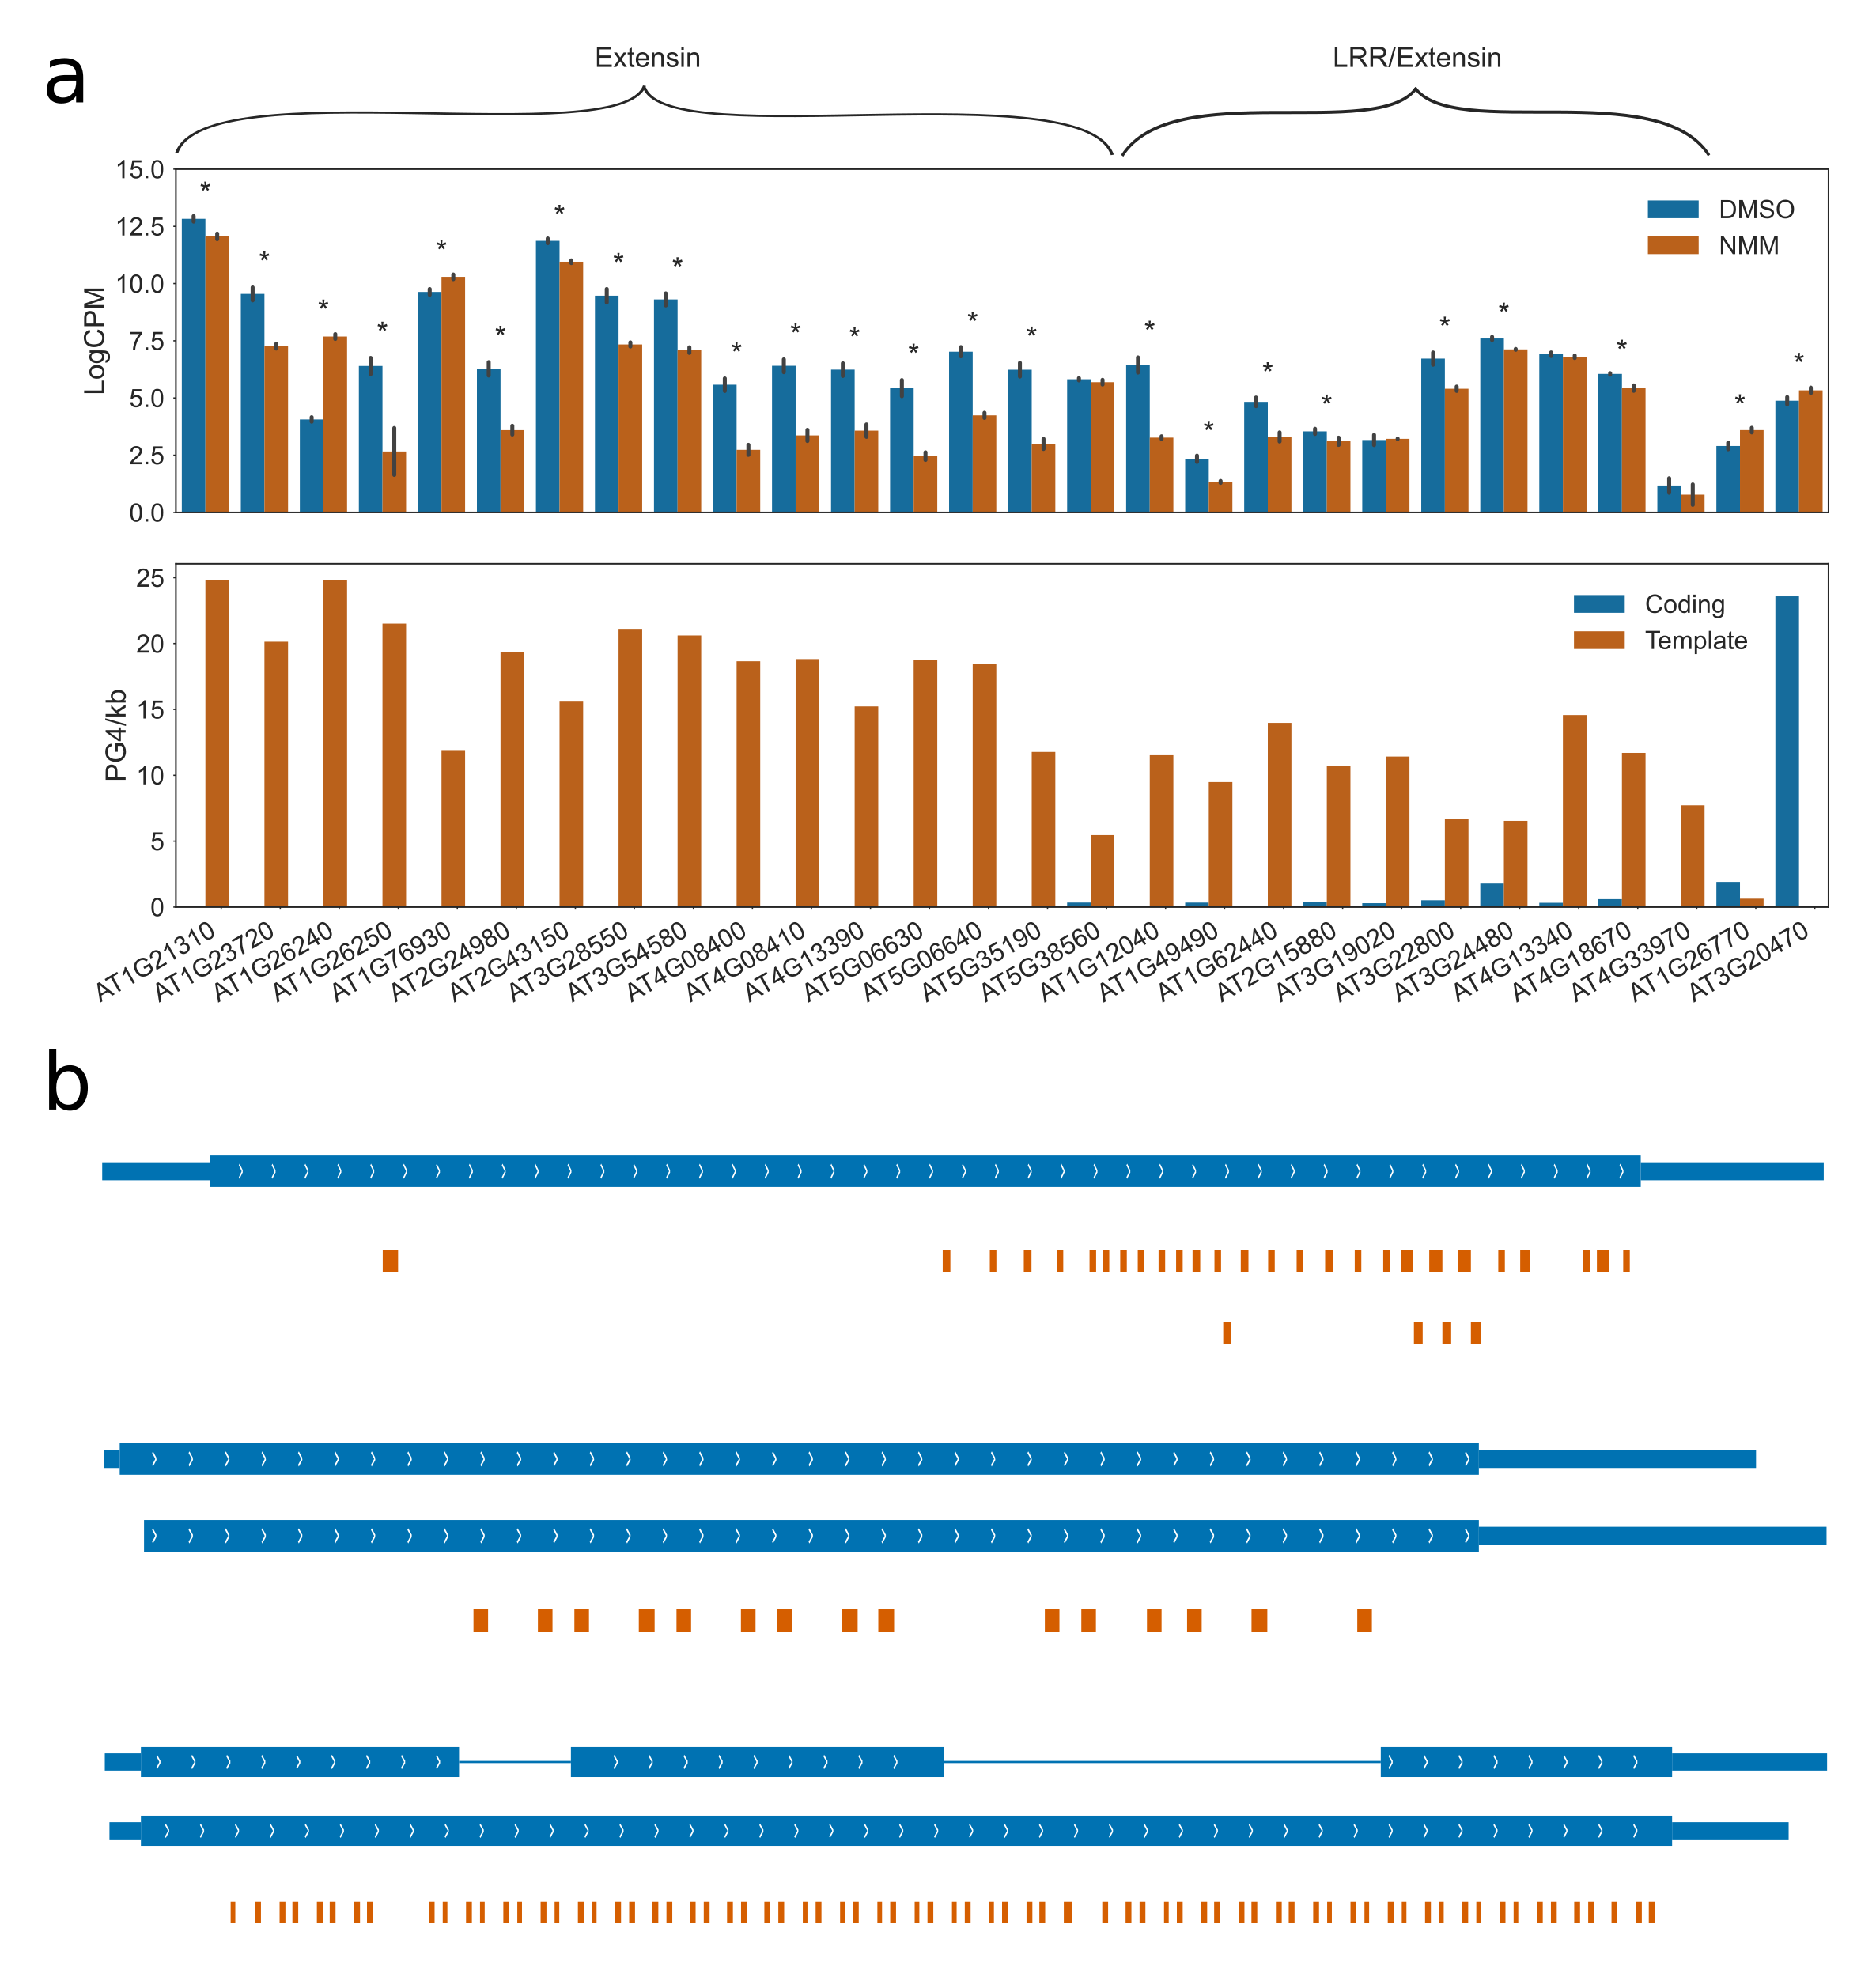
\includegraphics[width=\textwidth,height=562pt,keepaspectratio]{chapter_6/figures/extensin_gene_ontology_group_expression_g4s.png}
\caption[Expression and PG4 density of genes in the Cell Wall Structural Ontology group \texttt{GO:0005199}]{\textbf{Expression   and   PG4   density   of   genes   in   the   Cell   Wall   Structural   Ontology   group   \texttt{GO:0005199}}   \textbf{a)}   Panels   showing   gene   expression   (top   panel)   and   PG4   density   (bottom   panel)   for   genes   in   the   \texttt{GO:0005199}   group.   Expression   in   DMSO   (blue)   and   NMM   (orange)   conditions   is   shown   at   log2   counts   per   million   (from   root   RNAseq   dataset).   Errorbars   are   standard   deviation   of   three   biological   replicates.   Genes   which   are   differentially   expressed   with   FDR   <   0.05   are   labelled   with   asterisks.   In   PG4   panel,   the   exonic   PG4   density   per   kilobase   is   shown   separately   for   coding   (blue)   and   template   (orange)   strands   of   the   gene.   \textbf{b)}   Gene   tracks   showing   the   location   of   predicted   two   tetrad   PG4s   in   orange   for   (from   top   to   bottom)   LRX1,   EXT13,   and   EXT9.   Gene   models   from   Araport11   are   shown   in   blue.   In   gene   models,   thin   boxes   represent   untranslated   regions   (UTRs),   fat   boxes   represent   coding   regions   (CDS),   and   connecting   lines   represent   intronic   regions.   \label{ext_genes}}
\end{figure}

\newpage

From a search of the literature, we discovered that Extensin genes are
highly repetitive, proline rich proteins (Kieliszewski and Lamport,
1994; Showalter et al., 2010; Liu et al., 2016). These proteins
polymerise to function as a structural matrix in the protein component
of the plant cell wall (Lamport and Northcote, 1960; Lamport, 1965;
Showalter, 1993). In particular, we noted that these proteins are
characterised by large numbers of the SP3-5 repeat, which is made up of
the sequence \(Ser(Hyp)_{3-5}\), where Hyp is Hydroxy-proline, a proline
derivative (Showalter et al., 2010). Since the codon for proline is
\texttt{CCN}, the DNA which encodes SP4 and SP5 motifs will conform to
the two tetrad Quadparser motif on the template strand of the gene (Fig
\ref{cd_spec}a). This is the source of the PG4 density of Extensin
genes, and PG4 counts in these genes are well correlated with SP3-5
repeats (Fig \ref{ext_table}). Since the SP4 motif is required for the
function of the protein, and is restricted by the codon for proline,
these PG4s are ``hardcoded'' into the body of the gene.

\newpage

\begin{figure}[htbp]
\centering

\includegraphics[width=\textwidth,height=562pt,keepaspectratio]{chapter_6/figures/ext_family_showalter_table.png}
\caption[The Extensin gene family contains large numbers of hardcoded PG4s]{\textbf{The   Extensin   gene   family   contains   large   numbers   of   hardcoded   PG4s}   Table   showing   extended   Extensin   gene   family,   their   expression   patterns,   SP4   motif   counts,   PG4   counts   and   expression   during   NMM   treatment.   Adapted   from   Showalter   et   al. 2010   \label{ext_table}}
\end{figure}

\newpage

To demonstrate that the PG4 from Extensin genes could form a G4
structure in vitro we used circular dichroism spectroscopy (CD). We
performed these experiments at physiologically relevant temperatures for
Arabidopsis. An oligo representative of the SP4 repeat was designed
(\texttt{AGAGGTGGTGGTGGTATG}) using 3bp flanks upstream and downstream
of the PG4. CD showed the G4 oligo had peak absorbance at 260nm and
trough at 240nm, indicative of a parallel G4 structure (Fig
\ref{cd_spec}b). Removing the PG4 by mutating the sequence (mutated
sequence: \texttt{AGAGGTGATGGTGGTATG}) or removing potassium ions from
the buffer abolished this absorbance profile.

\newpage

\begin{figure}[htbp]
\centering
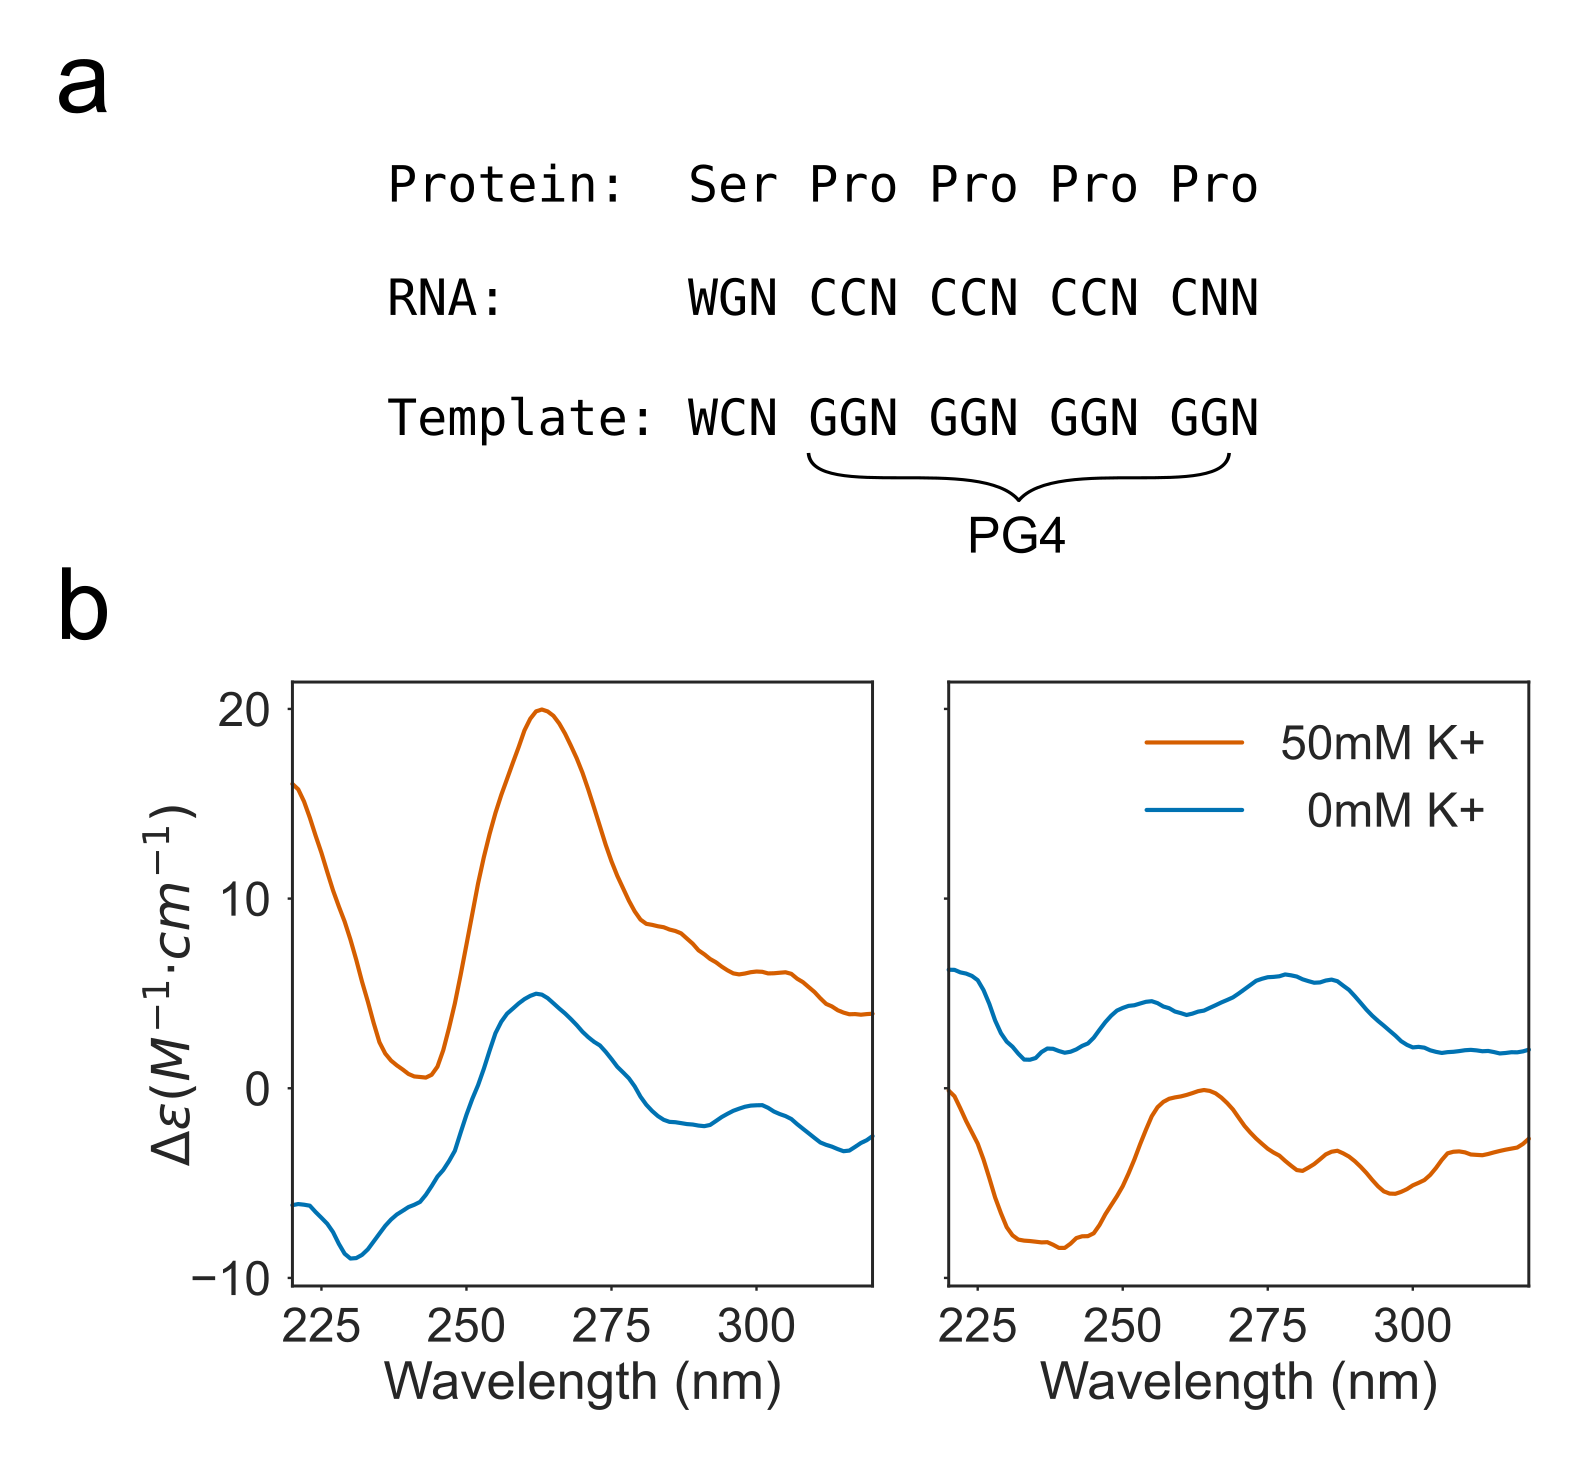
\includegraphics[width=\textwidth,height=562pt,keepaspectratio]{chapter_6/figures/cd_spectroscopy1.png}
\caption[The Extensin SP4 motif forms a G-Quadruplex \textit{in vitro}.]{\textbf{The   Extensin   SP4   motif   forms   a   G-Quadruplex   \textit{in   vitro} .}   \textbf{a)}   Schematic   showing   how   the   Extensin   SP4   protein   motif   hardcodes   a   two   tetrad   PG4   into   the   template   strand   of   the   gene   body.   \textbf{b)}   CD   spectroscopy   of   an   Extensin   repeat   sequence   (left)   and   a   mutated   control   which   does   not   conform   the   the   Quadparser   motif   (right)   show   that   the   Extensin   repeat   forms   a   G4   \textit{in   vitro} .   This   is   indicated   by   the   peak   in   ellipticity   at   260nm   and   the   trough   at   240nm,   which   are   characteristic   of   a   parallel   G4.   \label{cd_spec}}
\end{figure}

\newpage

\hypertarget{extensins-are-strongly-downregulated-by-nmm-and-berberine}{%
\subsection{Extensins are strongly downregulated by NMM and
Berberine}\label{extensins-are-strongly-downregulated-by-nmm-and-berberine}}

\label{ssec:extensin_downreg}

To confirm that the Extensin genes are downregulated by NMM, we
performed RNA extraction and quantitative RT-PCR (qPCR) on root tissue
from 7 day old Arabidopsis seedlings treated for 6 hours with NMM at
varying concentrations. EXT13 and LRX1 were chosen as representative
classical and chimeric Extensins, respectively (Showalter et al., 2010).
The change in expression of both genes upon treatment was negatively
correlated with the concentration of NMM applied (Fig
\ref{nmm_berb_qpcr}a). Treatment with the G4 intercalating drug,
Berberine, also caused strong downregulation of EXT13 and LRX1 (Fig
\ref{nmm_berb_qpcr}b). Since NMM and berberine are very different drugs
which stabilise G4s through different methods, taken together our
results suggest downregulation of Extensins is caused by G4
stabilisation.

\hypertarget{downregulation-of-extensins-by-nmm-is-translation-independent}{%
\subsection{Downregulation of Extensins by NMM is translation
independent}\label{downregulation-of-extensins-by-nmm-is-translation-independent}}

\label{sec:extensin_cyclohex}

To confirm whether downregulation of EXT13 and LRX1 by NMM was direct,
or the result of a perturbation the levels of a transcription factor, we
conducted qPCR experiments with combinatorial treatment of NMM and
Cyclohexamide (CHX). CHX is an inhibitor of translation which is
commonly used to determine whether interactions by transcription factors
on a gene are direct (Taverner et al., 2004; William et al., 2004). If
effects are indirect (i.e.~if the transcription factor of interest
regulates transcription of some intermediate transcriptional factor,
which regulates the gene of interest), then treatment with CHX will
prevent regulation, since any intermediate factors will not be able to
be translated. In the case of NMM treatment, this was used to see
whether NMM acts directly on EXT13 and LRX1 through G4 stabilisation, or
through other changes in the transcriptome. Seedlings were pretreated
with CHX for two hours, before NMM was added and treatment was continued
for another 6 hours. This experiment showed that that Extensin
downregulation by NMM still occurs even when translation is blocked,
suggesting that NMM acts directly upon the Extensin genes.

\newpage

\begin{figure}[htbp]
\centering
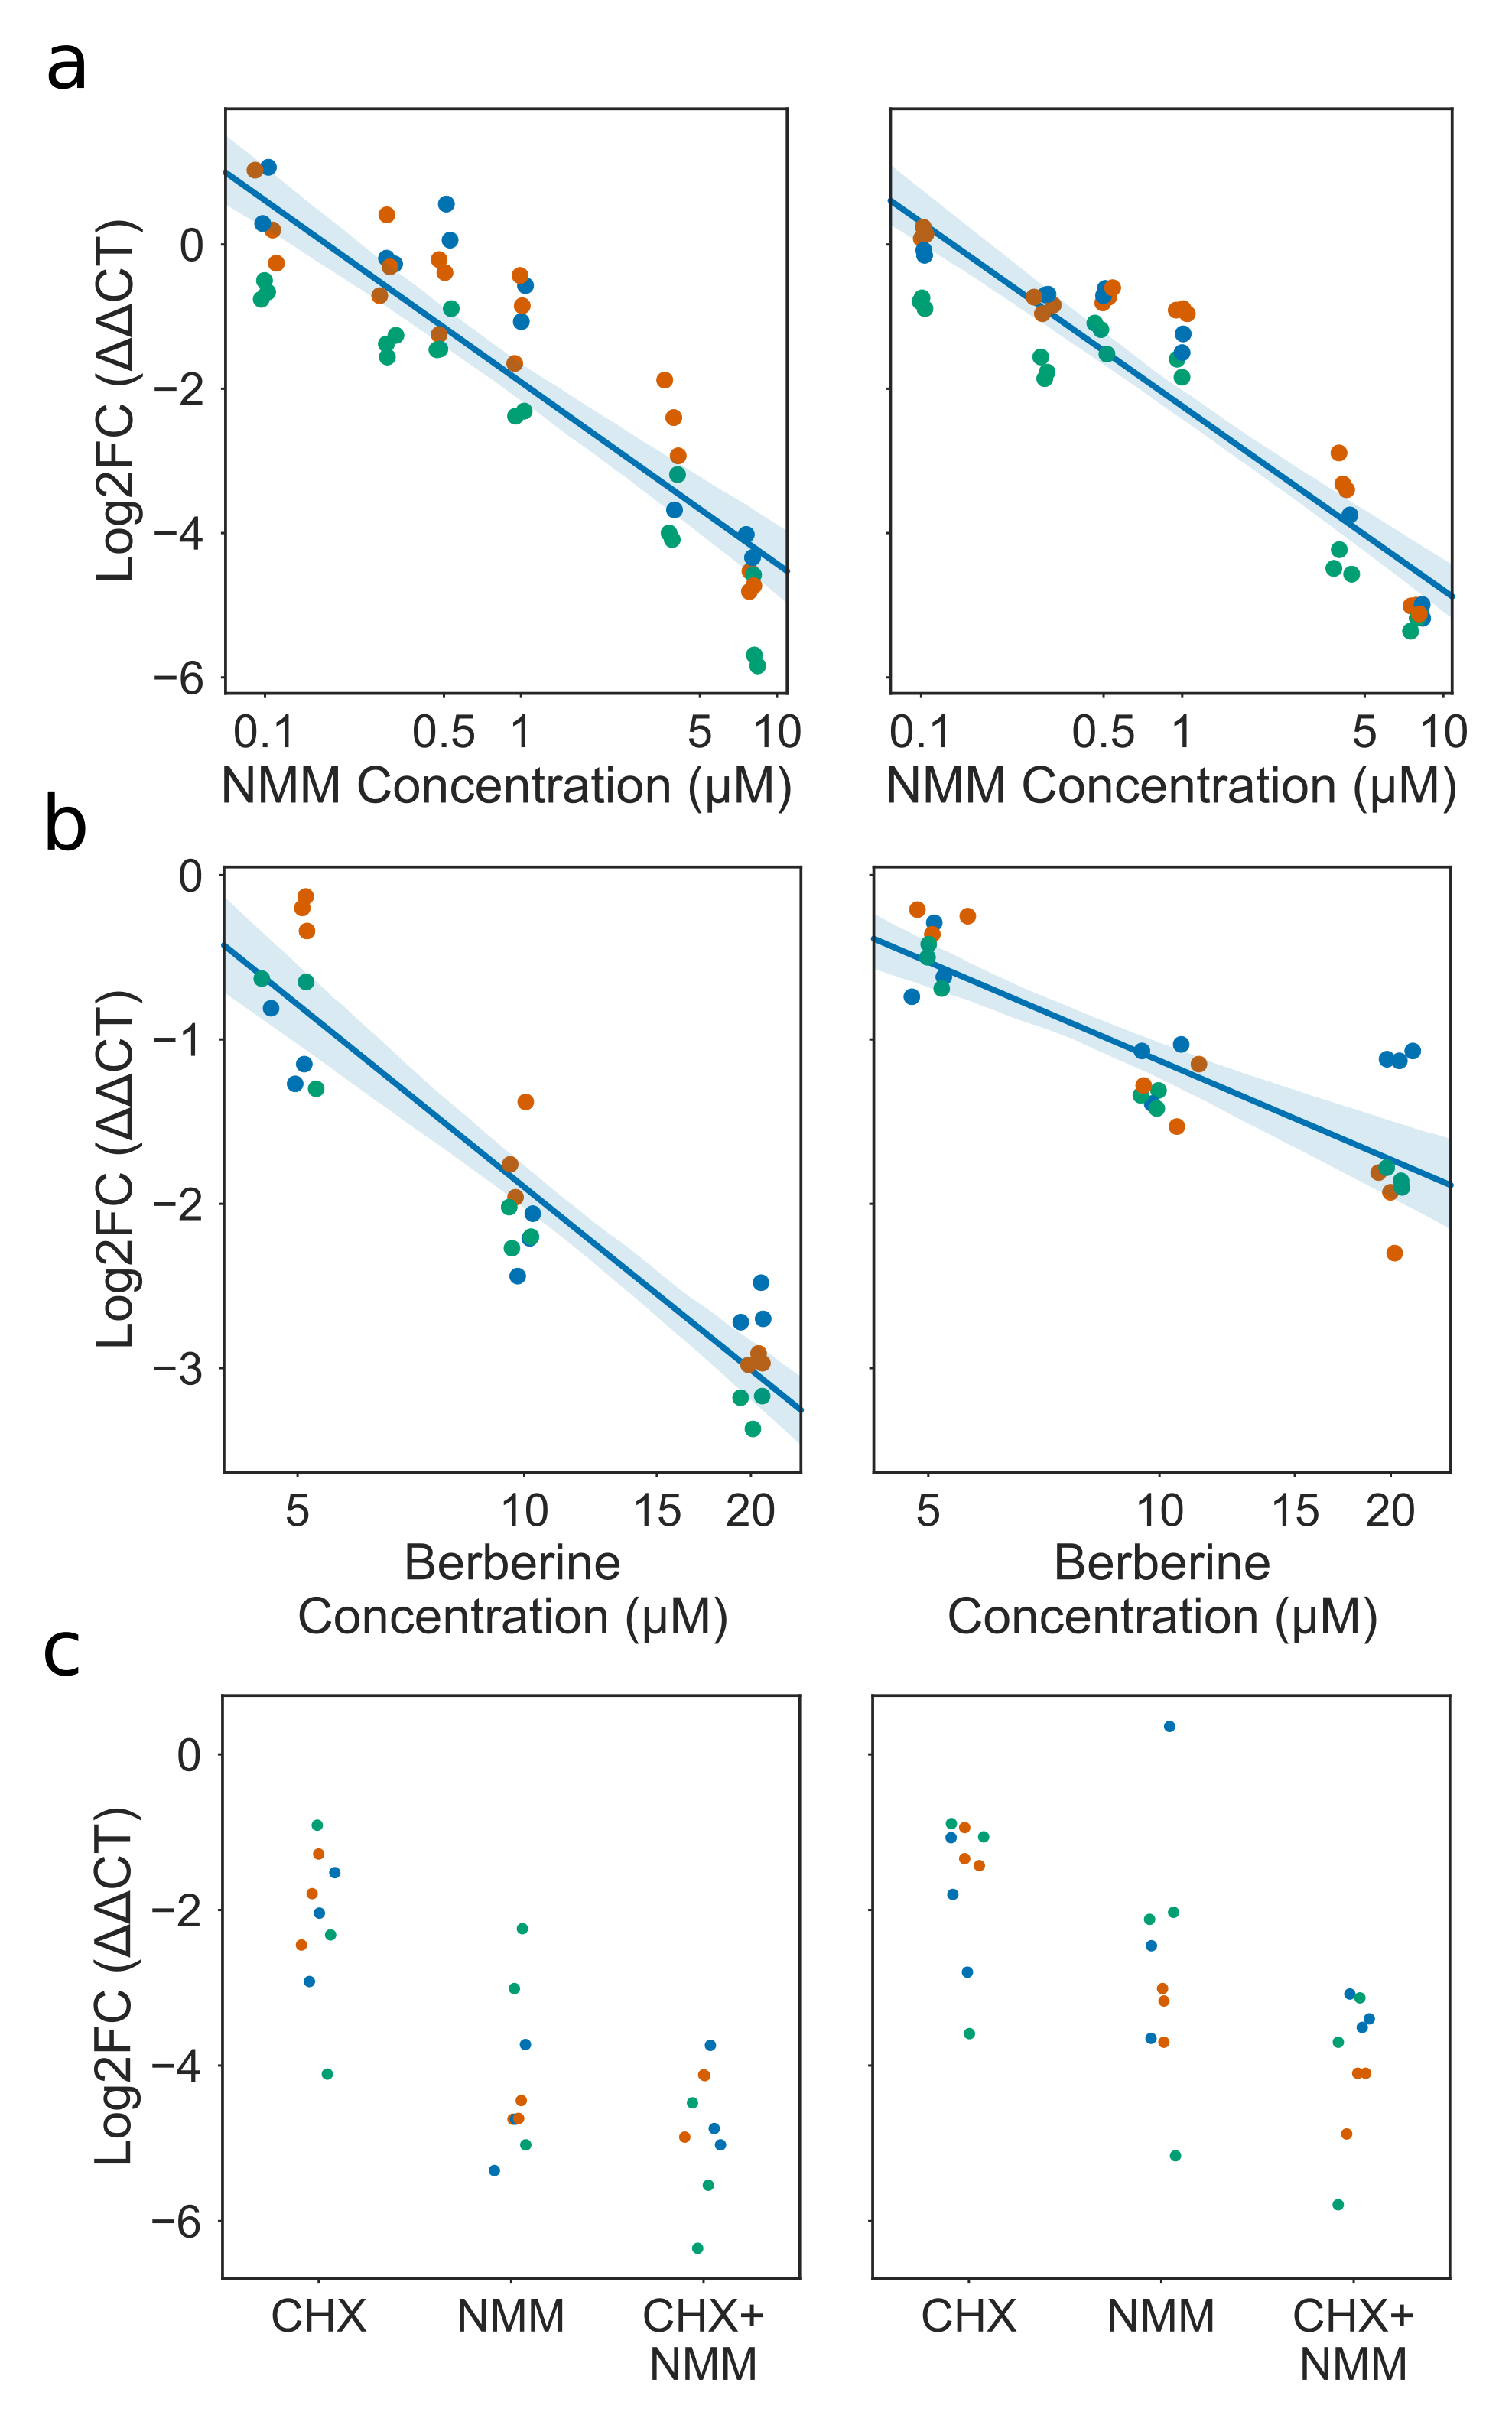
\includegraphics[width=\textwidth,height=562pt,keepaspectratio]{chapter_6/figures/ext13_lrx1_qpcr.png}
\caption[Expression of EXT13 and LRX1 during treatment with G4-binding ligands]{\textbf{Expression   of   EXT13   and   LRX1   during   treatment   with   G4-binding   ligands}   Scatter/strip   plots   showing   qPCR   results   for   EXT13   (left   panels)   and   LRX1   (right   panels).   Log2   fold   change   in   expression   (ΔΔCT)   of   Extensin   genes   decreases   with   increasing   concentrations   of   \textbf{a)}   NMM   and   \textbf{b)}   Berberine.   \textbf{c)}   NMM   downreguation   of   EXT13   and   LRX1   is   not   affected   by   concurrent   Cyclohexamide   treatment,   suggesting   a   mechanism   independent   of   translation.   For   all   panels,   each   point   is   a   single   technical   replicate,   and   colours   represent   different   biological   replicates.   A   small   amount   of   jitter   has   been   added   to   the   X   axis   for   better   visualisation   of   results.   \label{nmm_berb_qpcr}}
\end{figure}

\newpage

\hypertarget{rnaseq-suggests-extensin-genes-contain-exitronic-splice-sites}{%
\subsection{RNAseq suggests Extensin genes contain exitronic splice
sites}\label{rnaseq-suggests-extensin-genes-contain-exitronic-splice-sites}}

\label{ssec:extensin_splice_sites}

We noted from studying \emph{de novo} assembled splice isoforms from a
root specific RNAseq dataset (Li et al., 2016) that many of the Extensin
genes had large numbers of novel spliced isoforms. EXT9 was found to
have the most novel spliced forms of any gene in the dataset. These were
not present in the annotation. In fact, the majority of Extensin domains
are annotated in both TAIR10 and Araport11 as intronless. These splice
isoforms are presumably therefore a product of ``exitronic'' splicing
(Marquez et al., 2012, 2015), where sections of constitutive exons,
flanked on both sides by exonic sequence, are spliced out of a gene. We
hypothesised that these unusual exitrons could be a result of slow Pol
II elongation through PG4 dense regions, allowing splicing to occur at
weak splice sites.

A hallmark of most true splice junctions is the GT/AG intron motif,
which is the conserved canonical sequence in all higher eukaryotes,
including Arabidopsis (Fig \ref{splice_junct}a) (Mount, 1982; Shapiro
and Senapathy, 1987). To determine whether Extensin exitrons had
canonical splice motifs, we produced splice junction sequence logos for
predicted introns from the dataset produced by Li et al., for EXT9 and
LRX3, both of which were highly spliced. We found that splice junctions
in these genes had near universal GT/AG motifs (Fig
\ref{splice_junct}b). Upon inspection of the methods for Li et al.,
however we discovered that \texttt{CuffLinks} was used for \emph{de
novo} transcript assembly (Trapnell et al., 2012). Since the RNAseq
dataset is unstranded, \texttt{Cufflinks} requires the upstream mapping
tool (here, \texttt{STAR} (Dobin et al., 2013)) to annotate the
orientation of spliced reads using the intron motif (i.e.~positive
strand for GT/AG and negative strand for CT/AC). This setting means
reads which do not conform to the intron motif are discarded, leading to
serious bias.

To remove this bias, we remapped reads from the Li et al.~dataset using
STAR without filtering by intron motif. Since assemblers like
\texttt{CuffLinks} and \texttt{StringTie} (Pertea et al., 2015) require
strandedness information derived from the intron motif, transcript
assembly was not possible. Instead, we simply extracted spliced reads
aligning to EXT3 and LRX3 and identified all unique splice site starts
and ends. The corresponding sequences were then used to produce sequence
logos (Fig \ref{splice_junct}c). These logos showed only a weak
enrichment for the GT/AG motif in EXT9, and CT/AC in LRX1.

\newpage

\begin{figure}[htbp]
\centering
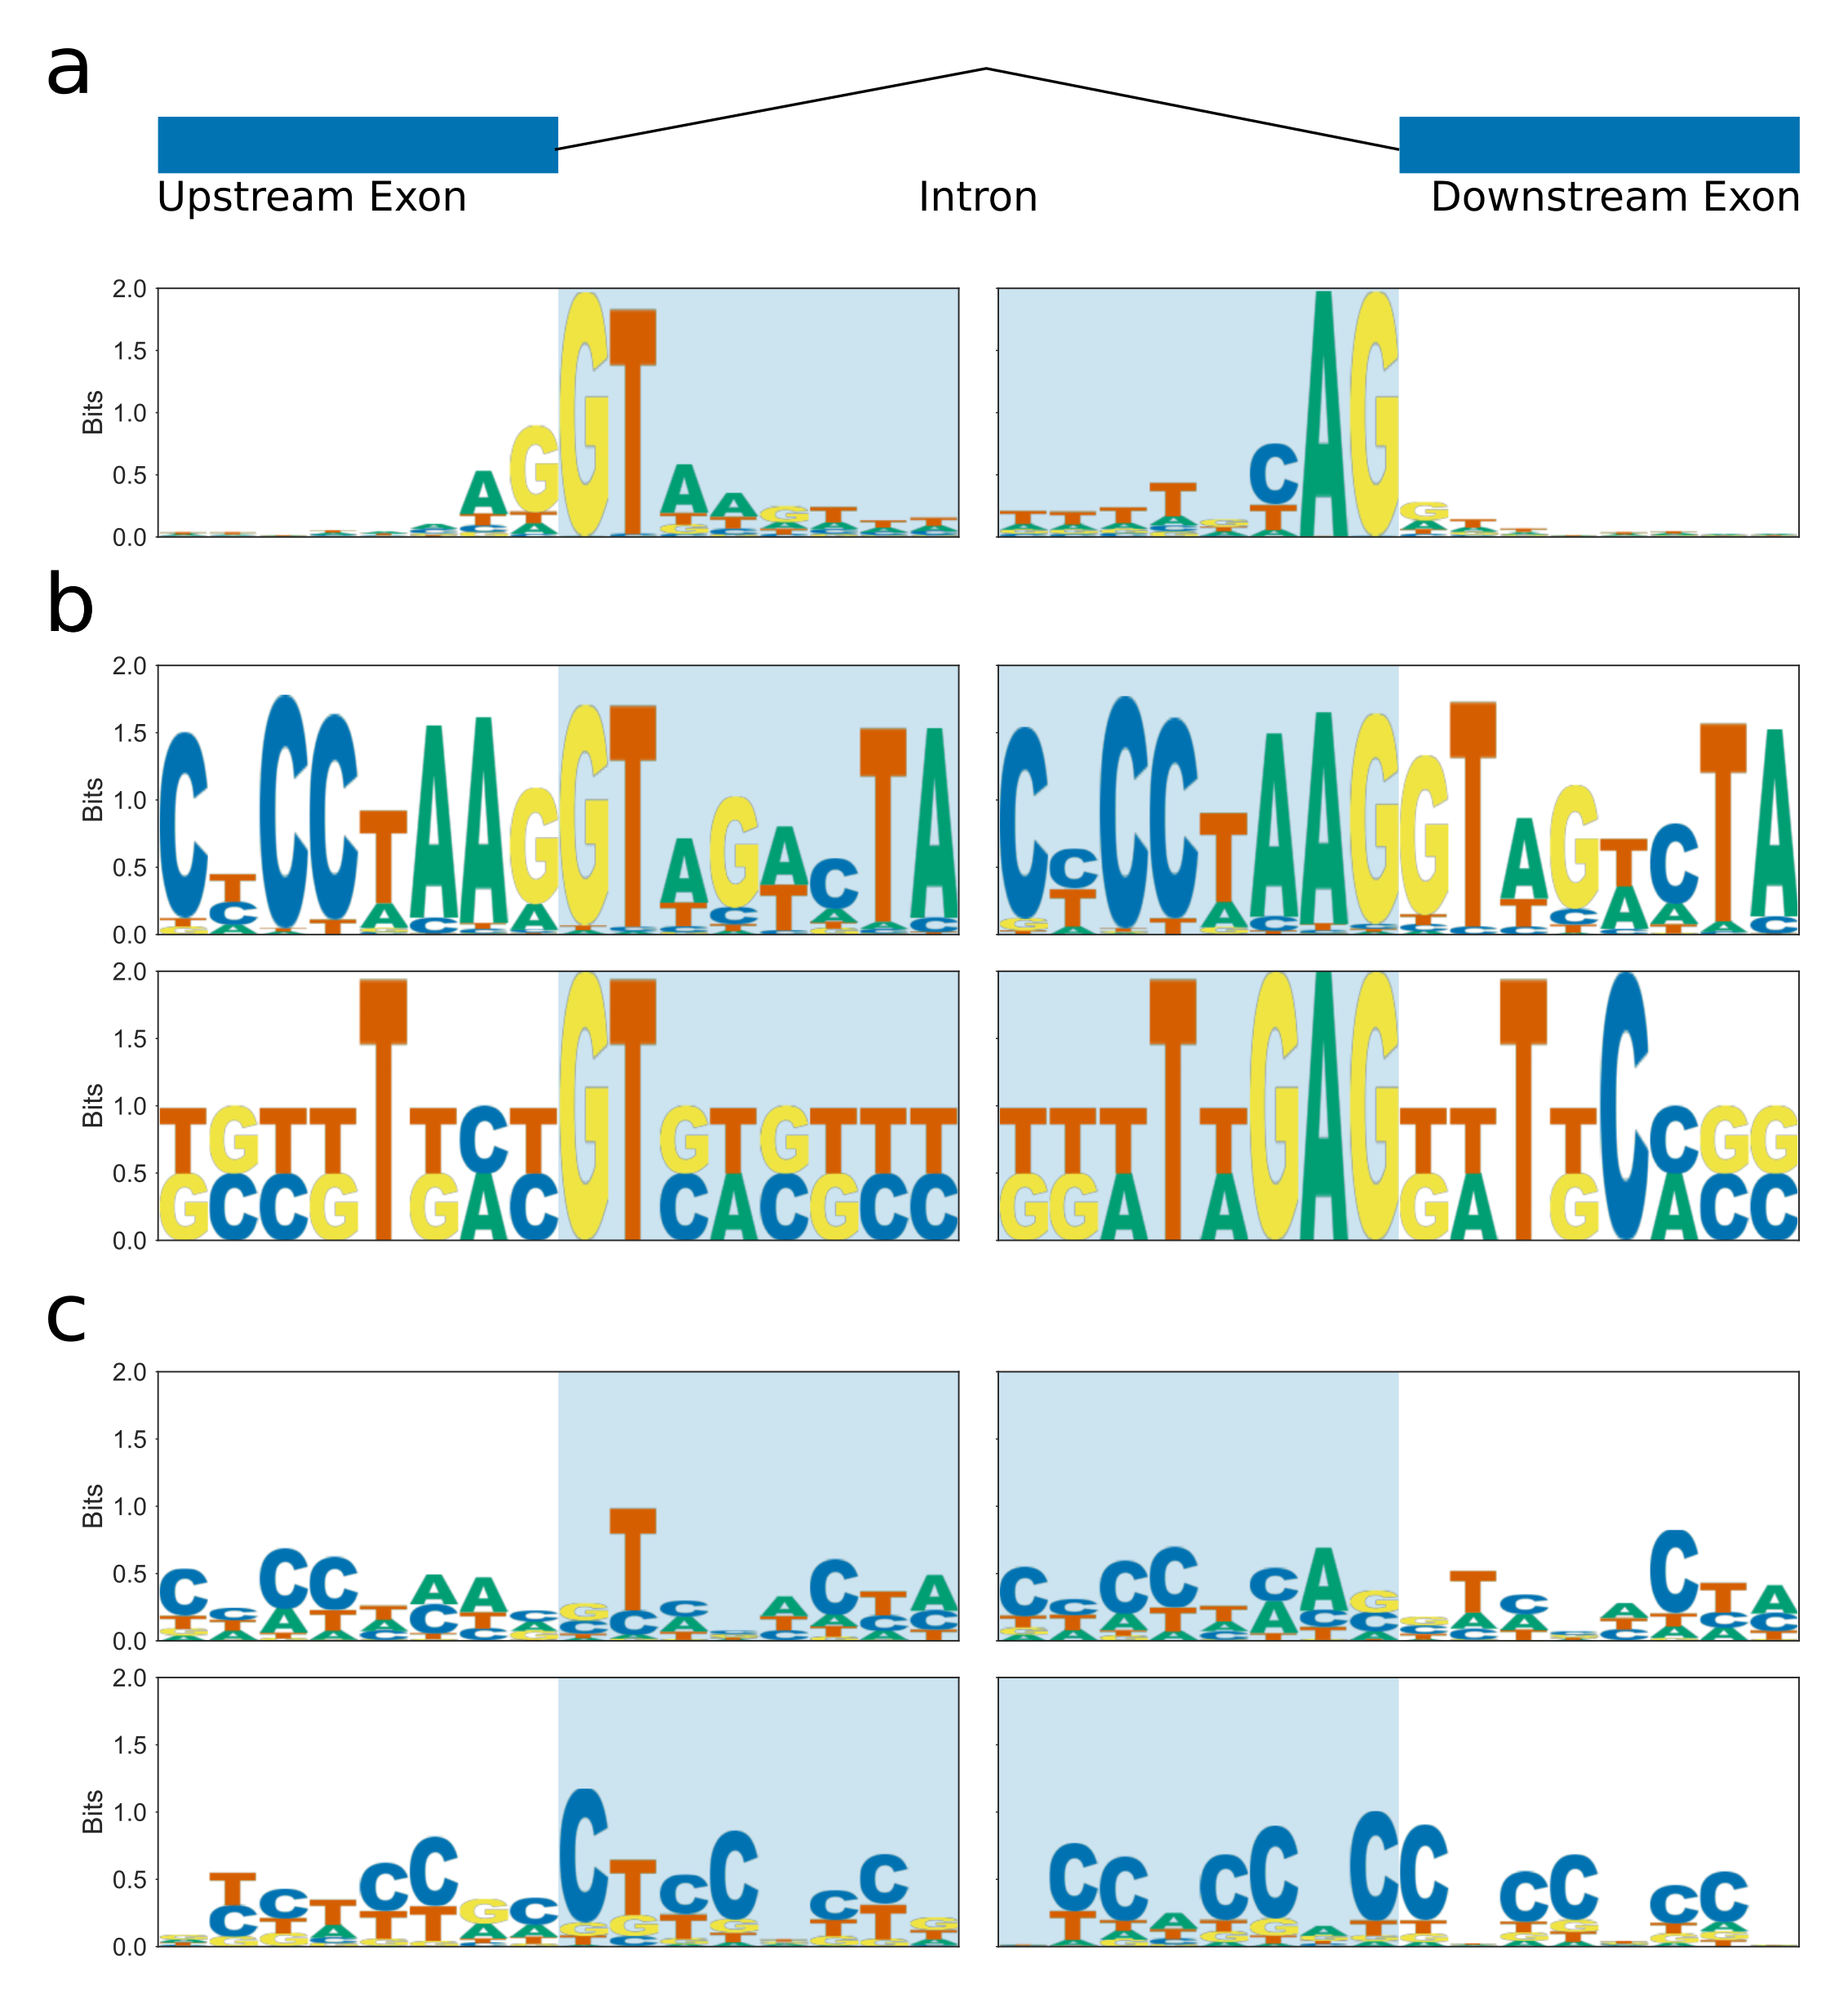
\includegraphics[width=\textwidth,height=562pt,keepaspectratio]{chapter_6/figures/splice_site_sequence_logo.png}
\caption[Splice junction motifs for EXT9 and LRX3]{\textbf{Splice   junction   motifs   for   EXT9   and   LRX3}   Sequence   logo   plots   showing   consensus   splice   site   sequences   around   donor   (left   panels)   and   acceptor   (right   panels)   splice   sites.   Putative   intronic   sequences   are   shown   on   shaded   blue   background.   \textbf{a)}   Splice   junction   consensus   sequence   logo   for   Arabidopsis,   calculated   from   junctions   in   the   Araport11   annotation.   \textbf{b)}   Splice   junction   consensus   sequence   logo   produced   from   \textbf{de   novo}   assembled   transcripts   (Li   et   al. 2016)   for   EXT9   and   LRX3.   \textbf{c)}   Splice   junction   consensus   sequence   logo   produced   from   unique   donor/acceptor   pairs   identified   from   spliced   reads   on   EXT9   and   LRX3.   \label{splice_junct}}
\end{figure}

\newpage

Since the Extensin exitrons appear in coding regions of DNA, if the
spliced out region is not a multiple of three, then the resulting mRNA
would be frameshifted, producing truncated and potentially deleterious
proteins. We therefore tested whether the spliced reads in EXT9 and LRX3
contained gaps which were multiples of three or not. For both genes,
almost all of the unique splice junction pairs were multiples of three
(Fig \ref{splice_frame}a-b). This could be evidence that these exitrons
are genuine and produce function gene products. On the other hand, we
noted that splicing tended to occur between regions with high protein
and DNA sequence level homology. EXT9, for example, is an incredibly
repetitive gene with high self-homology (Fig \ref{ext_mapp}a). These in
frame splice junctions could therefore simply be the result of mapping
errors from the spliced aligner \texttt{STAR} (Dobin et al., 2013),
which utilises heuristics which may result in some reads from contiguous
parts of the genome being mapped as spliced. If the homologous regions
which could cause mapping errors within a gene also have homology at the
protein level, as is the case in EXT9, then it is probable that
erroneously spliced reads would be a multiple of three in intron length.

If spliced reads mapping to EXT9 were the result of some systematic
error in mapping, one might not expect to see much variation in the
percent of reads mapping to a gene being spliced. We therefore
correlated the expression of EXT9 in each sample from the root RNAseq
dataset (measured in log2 counts per million or needs to be!) with the
percent of reads which mapped with a splice site. We found a slight
positive correlation between expression and splicing (Fig
\ref{splice_frame}c).

As a further precaution against these erroneous spliced mappings, we
performed read simulation for each sample in the root RNAseq dataset.
Put simply, the expression of each gene was quantified for each sample
by counting the number of mapped reads, then \texttt{Polyester} (an
Illumina sequencing read simulator) was run to generate reads from the
reference transcriptome with the same read counts (Frazee et al., 2015).
These simulated reads were then remapped with \texttt{STAR} using the
same parameters as the original mapping (Dobin et al., 2013). We then
performed a bootstrap analysis for EXT9 where we sampled one or more
real/simulated sample pairs, and counted the number of unique splice
donor/acceptor pairs that occurred in each. Junctions with the same
exonic flanking sequence (using 20bp overhangs) or with edit distance of
only one base were collapsed. Any junctions with flanking sequence that
appeared as a contiguous kmer in the reference sequence of EXT9 were
also removed. Despite this, we saw a consistently larger number of
unique donor/acceptor splice pairs in the real data than in the
simulated data (Fig \ref{splice_frame}d).

\newpage

\begin{figure}[htbp]
\centering
\includegraphics[width=\textwidth,height=562pt,keepaspectratio]{chapter_6/figures/splice_site_frame_and_simulation.png}
\caption[Splice junction motifs for EXT9 and LRX3]{\textbf{Splice   junction   motifs   for   EXT9   and   LRX3}   \textbf{a}   \&   \textbf{b)}   Frequency   barplots   showing   number   of   In/Out   of   frame   splice   junctions   for   EXT9   and   LRX3   respectively.   \textbf{c)}   Scatterplot   showing   percentage   of   reads   with   splicing   versus   log2   counts   per   million   for   EXT9.   \textbf{d)}   Bootstrapped   splicing   simulation   showing   number   of   unique   EXT9   splice   junctions   discovered   with   increasing   numbers   of   samples   for   real   root   RNAseq   data   versus   paired   simulated   RNAseq   data.   Errorbars   are   67\%   confidence   intervals.   \label{splice_frame}}
\end{figure}

\newpage

Since the Extensin genes are highly repetitive, this reduces the ability
of read aligners to map to them. This ``mappability'' can be quantified
using tools such as \texttt{GEM} which measure, for each genomic
position, how often the sequence kmer that is found there occurs in the
rest of the genome (Derrien et al., 2012). We utilised \texttt{GEM} to
score the mappability of the Arabidopsis genome, and compared the median
mappability score for extensin genes to the percent of spliced reads for
each gene. Only genes which were annotated as intronless (i.e.~no
constitutive introns, genes with exitrons were allowed) were included.
We found a clear negative correlation between mappability and the number
of mapped spliced reads (Fig \ref{ext_mapp}b). For EXT9, the regions
with lowest mappability are clearly those with the most annotated splice
sites, including in the Araport11 reference (Fig \ref{ext_mapp}c).

\newpage

\begin{figure}[htbp]
\centering
\includegraphics[width=\textwidth,height=562pt,keepaspectratio]{chapter_6/figures/ext9_dotplot_mappability.png}
\caption[Extensin genes with greater spliced mapped reads have low mappability]{\textbf{Extensin   genes   with   greater   spliced   mapped   reads   have   low   mappability}   \textbf{a)}   Dotplot   showing   self   homology   of   the   EXT9   cDNA   (unspliced   isoform).   Positional   identity   was   calculated   using   15bp   windows   across   the   gene.   Positions   with   identity   less   than   75\%   were   filtered   to   remove   noise   from   the   plot.   \textbf{b)}   Scatter   plot   showing   the   minimum   mappability   score   of   unspliced   Extensin   genes   against   the   percentage   of   spliced   reads   for   that   gene   in   mature   root   RNAseq   samples   (Li   et   al. 2016).   Errorbars   are   standard   deviation   of   three   biological   replicates.   \textbf{c)}   Gene   track   showing   the   mappability   score   across   EXT9   (orange).   Most   splice   forms   cross   these   low   mappability   regions,   including   in   the   reference   annotation   Araport11   (shown   in   blue).   \label{ext_mapp}}
\end{figure}

\newpage

\hypertarget{sanger-sequences-identifies-lrx1-and-ext9-splice-variants}{%
\subsection{Sanger sequences identifies LRX1 and EXT9 splice
variants}\label{sanger-sequences-identifies-lrx1-and-ext9-splice-variants}}

\label{ssec:extensin_sanger}

To experimentally confirm whether Extensin gene exitron splicing exists,
we performed RT-PCR of LRX1 and EXT9 mRNAs. PCR products of both genes
showed multiple products, characteristic of several spliced forms (data
not shown). PCR products which did not correspond to the full length of
the unspliced mRNA were gel extracted, cloned and sanger sequenced to
identify their origin. We identified a number of mRNA fragments
originating from the LRX1 and EXT9 genes. Alignment of these products
using \texttt{BLAT} identified a number of spliced isoforms in both
genes (Kent, 2002). To identify whether these isoforms contained
canonical splice sites, we produced sequence logos. Neither gene showed
a clear pattern conforming to the canonical intron motif GT/AG, though
the products from LRX1 showed the reverse complement of this pattern,
CT/AC.

\newpage

\begin{figure}[htbp]
\centering
\includegraphics[width=\textwidth,height=562pt,keepaspectratio]{chapter_6/figures/sanger_splice_variants.png}
\caption[Sanger sequencing of LRX1 and EXT9 cDNA identifies spliced forms]{\textbf{Sanger   sequencing   of   LRX1   and   EXT9   cDNA   identifies   spliced   forms}   \textbf{a)}   Gene   track   showing   aligned   sanger   sequencing   products   for   \textbf{a)}   LRX1   and   \textbf{b)}   EXT9.   Products   aligned   to   the   forward   strand   are   shown   in   green,   and   products   aligned   to   the   negative   strand   are   shown   in   orange.   Gene   models   are   from   the   Araport11   annotation.   \textbf{c)}   Sequence   logos   for   sanger   product   splice   junctions   for   LRX1   (top   panel)   and   EXT9   (lower   panel).   \label{sanger}}
\end{figure}

\newpage

\hypertarget{nmm-treated-plants-do-not-have-increased-splicing-of-extensin-genes}{%
\subsection{NMM treated plants do not have increased splicing of
Extensin
genes}\label{nmm-treated-plants-do-not-have-increased-splicing-of-extensin-genes}}

\label{ssec:extensin_nmm_splice}

We hypothesise that G4s cause the exitronic splicing of Extensin genes,
by slowing down Pol II elongation. To test whether increased
stabilisation of G4s changes this splicing pattern, we performed RNAseq
of root tissue from plants treated with NMM using 220bp paired reads, to
identify novel splicing isoforms. Mapping parameters for \texttt{STAR}
(Dobin et al., 2013) were made more stringent than defaults in an
attempt to increase the precision of mapping over Extensin genes without
attenuating recall of splice junctions too strongly. A common method for
conducting differential splicing analysis is to use differential exon
usage methods such as \texttt{DEXseq} (Anders et al., 2012). This is
sometimes conducted on exon ``chunks'' which are the contiguous genomic
ranges which each appear in a distinct set of transcripts of a gene.
Since there are many overlapping exitrons in the Extensin genes, these
chunks would be extremely short and be complex to interpret.
Furthermore, if spliced transcripts are in lower abundance than full
length transcripts, a large change in the use of a particular exitron
may only lead to a small change in the expression of the exon chunk
which is being spliced out. We therefore opted for counting the number
of reads which support each unique junction in a gene (junction counts),
and performing differential junction usage on this. The downside to this
analysis is that the number of reads supporting each junction may be
lower than the number per exon, leading to reduced power to detect
differential usage.

In order to perform junction level differential splicing analysis, we
identified all spliced reads with the correct first-in-pair strand
orientation overlapping each gene. Only splice junctions with at least
20 supporting reads total across the 6 samples were kept for analysis.
Splice junctions were categorised into five types based on how they
related to the flattened reference annotation in Araport11:
constitutive, alternative, retained intron/exitronic, exon skipping, or
other. See Fig \ref{diff_junc}a legend for an explanation of these
different categories.

We performed differential junction usage using \texttt{limma-voom} and
\texttt{limma-diffSplice} (Law et al., 2014; Ritchie et al., 2015).
Using an FDR threshold of 0.2 and an absolute fold change threshold of
0.5, we identified 338 junctions in 302 genes with increased use during
NMM treatment, and 189 junctions in 162 genes with decreased usage. 27
genes contained junctions which showed both increased and decreased
usages, i.e.~some type of switching. None of the junction isoforms
identified in the Extensin genes were significantly differentially
utilised, however.

\newpage

\begin{figure}[htbp]
\centering
\includegraphics[width=\textwidth,height=562pt,keepaspectratio]{chapter_6/figures/diff_splice_results.png}
\caption[Differential Junction Usage during NMM treatment]{\textbf{Differential   Junction   Usage   during   NMM   treatment}   \textbf{a)}   Schematic   showing   the   five   classes   used   to   categorise   splice   junctions   based   on   flattened   reference   annotation.   Junctions   which   are   present   as   introns   in   the   reference   are   labelled   constitutive   junctions.   Constitutive   junctions   which   cause   skipping   of   an   exon   are   labelled   skipping   junctions.   Junctions   which   share   a   donor   or   acceptor   site   with   one   in   the   reference   are   labelled   alternate   junctions.   Junctions   which   are   wholly   contained   within   a   single   exon   of   the   reference   are   labelled   retained/exitronic   junctions.   Finally,   junctions   which   share   no   donor   or   acceptor   with   the   reference   and   span   a   mixture   of   exonic   and   intronic   sequence   are   labelled   " other .   \textbf{b)}   Violin   plot   showing   distribution   of   average   expression   in   log2   counts   per   million   for   each   junction   class.   \textbf{c)}   Proportion   of   junction   in   each   class   for   all   splice   junctions   vs. those   with   significantly   increased   or   decreased   usage   during   NMM   treatment   (Absolute   logFC   >   0.5,   FDR   <   0.2).   \textbf{d)}   Categorisation   of   detected   junctions   in   Extensin   genes.   \label{diff_junc}}
\end{figure}

\newpage

The linear model fit by \texttt{diffSplice} is looking for differences
in the usage of a junction relative to the usage of the rest of the
junctions in that gene. It is possible therefore, if utilisation of all
splice junctions in the Extensin genes were changed by a relatively
similar amount, that \texttt{diffSplice} would not detect any
differentially utilised junctions. We therefore examined the total
percentage of reads mapping to each Extensin gene which were exitronic,
and looked to see if this percentage changed during NMM treatment.
Despite large gene-level effects on many Extensin genes with Extronic
splicing (Fig \ref{perc_spliced}a, there was no strong effect on the
overall level of spliced reads mapping to these genes (Fig
\ref{perc_spliced}b), suggesting that either NMM does not affect the
splicing of Extensins, only the expression, or that spliced mapping to
these genes is a systematic mapping error that occurs at approximately
the same rate per gene regardless of the read count.

\newpage

\begin{figure}[htbp]
\centering
\includegraphics[width=\textwidth,height=562pt,keepaspectratio]{chapter_6/figures/extensin_percent_spliced.png}
\caption[NMM does not cause significant changes in the amount of Exitronic Splicing of Extensins]{\textbf{NMM   does   not   cause   significant   changes   in   the   amount   of   Exitronic   Splicing   of   Extensins}   Barplots   showing   \textbf{a)}   gene   expression   in   log2   counts   per   million,   and   \textbf{b)}   percentage   of   reads   exhibiting   Exitronic   splicing,   for   expressed   Extensin   genes   with   an   average   of   at   least   5\%   spliced   reads.   Levels   during   mock   (DMSO)   treatment   are   shown   in   blue,   and   levels   during   NMM   treatment   are   shown   in   orange.   Ordering   of   genes   (by   average   percent   spliced)   in   upper   and   lower   panels   is   matched.   Errorbars   are   standard   deviation   of   three   biological   replicates.   \label{perc_spliced}}
\end{figure}

\newpage

\hypertarget{discussion-2}{%
\section{Discussion}\label{discussion-2}}

\label{sec:extensin_discuss}

We have identified a new family of G4 regulated genes: the Extensins.
This is an extremely unusual and difficult to study family of genes, due
to high levels of self homology and paralogy. The repetition which makes
Extensins less tractable is also what makes them interesting to us: it
is caused by large numbers of poly-proline rich sequences, called SP4
motifs, which give rise to template stranded two tetrad PG4s. Our
\emph{in vitro} CD spectroscopy work suggests that these PG4 sequences
indeed form G4s which may be stable in the physiological temperature
range that Arabidopsis lives at.

SP4 motifs are found throughout the coding regions of Extensin domains,
usually in regularly spaced patterns. Since they contain large numbers
of the motif, Extensins are some of the most PG4 dense genes in
Arabidopsis, potentially in any organism. The density of PG4 sequences
may also lead to large combinatorial increases in the G4 topologies that
can form: an analysis of all the possible overlapping PG4 structures in
Extensins suggests that some have more than 500 potential conformations
per kilobase. Greater numbers of potential G4 conformations of these
sequences may increase the entropy and therefore the thermodynamic
stability of the folded population. This seems likely to have biological
implications in transcription or regulation of the genes.

The majority of Extensin family genes exhibit a sharp reduction in gene
expression when plants are treated with the G4-stabilising ligand NMM.
We have demonstrated this robustly through independent analyses of
microarray, RNAseq and qPCR data. Furthermore, treatment with another G4
binding ligand, Berberine, also downregulated selected Extensins, shown
by qPCR. Berberine has a very different structure and binds G4s through
a totally different mechanism to NMM, suggesting that this is likely to
be a direct G4 effect. As we showed in \autoref{chap:global_nmm}, NMM
appears to have a strong global effect on the expression of genes with
template stranded PG4s. Whilst this effect may be in part attributable
to the Extensin genes, it is not solely due to them, since 50\% more NMM
downregulated genes than might be expected by chance contain template
stranded PG4s. Our hypothesis is that template stranded PG4s cause
blockages which slow the progression of Pol II along the gene during
transcription. When NMM is added, this may cause increased slowing or
even premature termination of transcription, resulting in decreased
expression. We demonstrated that the effect of NMM is translation
independent (i.e.~not caused by transcription factor activity) by
treating plants with both Cyclohexamide and NMM at the same time, and
showing that NMM still caused downregulation.

Examination of \emph{de novo} assembled splice isoforms collated from
many RNAseq samples in Li et al 2016 led us to speculate about splicing
of Extensin genes (Li et al., 2016). EXT9 was found to have the most
different splice isoforms of any gene in this dataset. These splice
sites tended to occur within exonic sequence and remove regions which on
the template strand were PG4 rich. Analysis of how these splicing
patterns might affect the protein encoded by the mRNA showed that they
were multiples of three and would not cause frameshifts. Instead they
would simply cause greater variation in the length of protein products.
This is an intriguing idea since the Extensins are structural components
of the cell wall protein matrix, and it is possible that different
lengths of building block might result in differences in flexibility of
the wall. Furthermore, previous work has shown that truncated versions
of LRX1 with fewer SP4 repeats still function and are able to rescue an
\emph{lrx1} null mutation (Baumberger et al., 2001). It became clear,
however, that the number and type of splice junctions which could be
discovered in Extensin genes was highly dependent on parameters used in
mapping, suggesting that at least some of these splice junctions are
spurious and caused by technical error.

To try to identify true splice isoforms of Extensin genes, we performed
RNAseq, using longer 220bp paired end reads to attempt to capture more
splice junctions and reduce the number of multimapping reads. Since
splicing occurs co-transcriptionally, and Pol II elongation speed is
linked to utilisation of weak splice sites, we hypothesised that
splicing of Extensins might be controlled by formation of G4s which slow
down transcription. We therefore also performed RNAseq with NMM treated
plants to see how G4 stabilisation affects splicing. Our RNAseq dataset
identified large numbers of potential splice variants, however again
many of these did not have the hallmarks of canonical splice junctions,
and their abundances were highly sensitive to changes in mapping
parameters, suggesting the possibility of some technical defect.
Furthermore we did not see any strong or consistent change in the
percentage of spliced reads identified when plants were treated with
NMM, despite some very strong changes in the expression of Extensin
genes as a whole. Despite these negative results, we were able to
identify PCR products from cDNA which appeared to be truncated forms of
both EXT9 and LRX1. Again, these products did not have any consistent
traits of splice variants. One explanation for these results, and the
results of the RNAseq, could be artefacts introduced during PCR
amplification. These can occur in repetitive regions due to incorrect
annealing of single stranded DNA and can result in deletions or
expansions. To overcome these issues in the future, the ideal techniques
for detecting true splice forms would be Northern blots on a gene by
gene basis, or using direct RNA Nanopore sequencing for global
identification.

\newpage

\hypertarget{discussion-3}{%
\chapter{Discussion}\label{discussion-3}}

We have presented an in-depth analysis of the distribution of genic G4s
in \emph{Arabidopsis thaliana}. As demonstrated by other groups, we
found the levels of potential three tetrad G4s in Arabidopsis are low
compared to the number of two tetrad PG4s (Mullen et al.~2010). Our
analysis also shows that Arabidopsis genes have high levels of template
stranded PG4 sequences, both in the 5' UTR and in the start codon
proximal end of the CDS. These levels constitute an enrichment over what
would be expected in random sequence with identical GC content and
dinucleotide frequencies, and random sequences which could encode the
same protein. Furthermore, we show that many G4s are fully or partially
hardcoded by protein sequence, suggesting that in some cases protein
sequence might be influenced by the G4 forming potential of the DNA.
Poly-glycine and poly-proline motifs, which induce hardcoded PG4s on the
coding and template strands respectively, were found to account for a
large number of Arabidopsis CDS PG4s. We also showed, however, that the
percentage of non-hardcoded template strand PG4s is greater at the start
codon proximal end of the CDS, indicating codon selection to increase G4
forming potential in this part of the gene body. We hypothesised that
G4s may arise in the start of CDSs when 5'UTRs are too short to contain
them, however we did not find any correlation between the presence of
G4s in the first 100bp of the CDS, and the length of the 5' UTR,
suggesting that this is not the case.

Our microarray and RNAseq datasets have shown reproducibly that
treatment of Arabidopsis with the G4 stabilising ligand NMM causes
widespread changes in gene expression. Genes which contain template
stranded two tetrad G4s in their 5' UTRs and CDS regions tended to be
downregulated by NMM treatment. Genes with coding strand G4s in the gene
body were not as strongly affected, indicating a potential mechanism
involving the template strand. Since the template, or non-transcribed,
strand is the one scanned by Pol II during transcription, we
hypothesised that stabilised G4s on the template strand may form
blockages that prevent the elongation of PolII, whilst coding strand G4s
will not. These blockages may result in premature termination of
transcription. We found that large numbers of clustered PG4s in a 200bp
window were also indicative of reduced expression, suggesting that
clusters of stabilised G4s are more problematic to Pol II than single
G4s.

We analysed publicly available Pol II ChIP-chip data (Chodvarupu et
al.~2012) to show that PG4 dense genes have altered Pol II profiles,
with greater Pol II density at the TSS proximal end of genes and lower
Pol II density at the TSS distal end, compared to the profiles of most
over genes. This could be considered indicative of a slowing or pausing
of Pol II over G4 dense regions under normal conditions, i.e.~not in the
presence of G4 stabilising agents. We did not see higher ratios of reads
originating from nascent to mature mRNAs on PG4 dense genes, however,
suggesting that this slowing does not naturally result in premature
termination or degradation. Despite this, it is well documented that Pol
II elongation speed affects co-transcriptional processes such as
splicing, and so Pol II slowing by G4s may affect these processes.

A family of poly-proline rich protein-coding genes, called the
Extensins, were identified as strongly downregulated by NMM. The
Extensins were found to be extremely PG4 rich on the template strand,
containing as many as X different overlapping PG4 registers per gene. We
found that Extensin genes are also downregulated by Berberine, another
G4 binding agent, suggesting that downregulation is indeed caused by G4
stabilisation and not by any off-target effects. Furthermore,
downregulation by NMM treatment was not affected by pre-treatment with
the translation inhibitor cyclohexamide, suggesting that NMM has a
direct effect on Extensin gene expression.

The Extensins have relatively high levels of spliced reads mapping to
them, despite being mostly single exon genes. These exitronic splice
junctions tend to be over the PG4 rich regions of the gene. We
hypothesised that these spliced reads may be the result of Pol II
slowing at G4 rich regions of the gene, which allows co-transcriptional
splicing to occur at weak splice junctions. Because of the
repetitiveness of the Extensin genes, it is possible that some of these
spliced reads might result from mapping errors, however we did not find
as many unique splice junctions in simulated datasets as in the real
RNAseq data. Furthermore, were able to isolate, clone, and sanger
sequence some of these spliced transcripts. None of these truncated
transcripts appeared to have canonical splice junction sequences,
however, possibly indicating that they may be PCR artefacts. In future
we could use Nanopore direct RNA sequencing, which has no PCR step and
is able to sequence whole mRNA molecules regardless of repetitiveness,
to identify whether the Extensin exitrons are real or artefactual.

\newpage
\section*{References}
\addcontentsline{toc}{chapter}{References}{}

\hypertarget{refs}{}
\leavevmode\hypertarget{ref-Abadi2016}{}%
Abadi, M., Agarwal, A., Barham, P., Brevdo, E., Chen, Z., Citro, C.,
Corrado, G.S., Davis, A., Dean, J., Devin, M., et al. (2016).
TensorFlow: Large-Scale Machine Learning on Heterogeneous Distributed
Systems.

\leavevmode\hypertarget{ref-Aho1988}{}%
Aho, A.V., Kernighan, B.W., and Weinberger, P.J. (1988). The AWK
programming language (Addison-Wesley Pub. Co).

\leavevmode\hypertarget{ref-Alipanahi2015}{}%
Alipanahi, B., Delong, A., Weirauch, M.T., and Frey, B.J. (2015).
Predicting the sequence specificities of DNA- and RNA-binding proteins
by deep learning. Nature Biotechnology \emph{33}, 831--838.

\leavevmode\hypertarget{ref-Ambros2004}{}%
Ambros, V. (2004). The functions of animal microRNAs. Nature \emph{431},
350--355.

\leavevmode\hypertarget{ref-Ambrus2005}{}%
Ambrus, A., Chen, D., Dai, J., Jones, R.A., and Yang, D. (2005).
Solution Structure of the Biologically Relevant G-Quadruplex Element in
the Human c-MYC Promoter. Implications for G-Quadruplex Stabilization.
Biochemistry \emph{44}, 2048--2058.

\leavevmode\hypertarget{ref-Ambrus2006}{}%
Ambrus, A., Chen, D., Dai, J., Bialis, T., Jones, R.A., and Yang, D.
(2006). Human telomeric sequence forms a hybrid-type intramolecular
G-quadruplex structure with mixed parallel/antiparallel strands in
potassium solution. Nucleic Acids Research \emph{34}, 2723--2735.

\leavevmode\hypertarget{ref-Ameur2011}{}%
Ameur, A., Zaghlool, A., Halvardson, J., Wetterbom, A., Gyllensten, U.,
Cavelier, L., and Feuk, L. (2011). Total RNA sequencing reveals nascent
transcription and widespread co-transcriptional splicing in the human
brain. Nature Structural and Molecular Biology \emph{18}, 1435--1440.

\leavevmode\hypertarget{ref-Anders2012}{}%
Anders, S., Reyes, A., and Huber, W. (2012). Detecting differential
usage of exons from RNA-seq data. Genome Research \emph{22}, 2008--2017.

\leavevmode\hypertarget{ref-Andorf2014}{}%
Andorf, C.M., Kopylov, M., Dobbs, D., Koch, K.E., Stroupe, M.E.,
Lawrence, C.J., and Bass, H.W. (2014). G-Quadruplex (G4) motifs in the
maize (Zea mays L.) genome are enriched at specific locations in
thousands of genes coupled to energy status, hypoxia, low sugar, and
nutrient deprivation. Journal of Genetics and Genomics \emph{41},
627--647.

\leavevmode\hypertarget{ref-Collette2013}{}%
Andrew Collette (2013). Python and HDF5 (O'Reilly Media).

\leavevmode\hypertarget{ref-Andrews2010}{}%
Andrews, S. (2010). FastQC: a quality control tool for high throughput
sequence data. Available Online at:
Http://Www.bioinformatics.babraham.ac.uk/Projects/Fastqc.

\leavevmode\hypertarget{ref-Arora2008}{}%
Arora, A., and Maiti, S. (2008). Effect of loop orientation on
quadruplex - TMPyP4 interaction. Journal of Physical Chemistry B
\emph{112}, 8151--8159.

\leavevmode\hypertarget{ref-Ayrapetov2014}{}%
Ayrapetov, M.K., Gursoy-Yuzugullu, O., Xu, C., Xu, Y., and Price, B.D.
(2014). DNA double-strand breaks promote methylation of histone H3 on
lysine 9 and transient formation of repressive chromatin. Proceedings of
the National Academy of Sciences \emph{111}, 9169--9174.

\leavevmode\hypertarget{ref-Balasubramanian2011}{}%
Balasubramanian, S., Hurley, L.H., and Neidle, S. (2011). Targeting
G-quadruplexes in gene promoters: A novel anticancer strategy? Nature
Reviews Drug Discovery \emph{10}, 261--275.

\leavevmode\hypertarget{ref-Bang1910}{}%
Bang, I. (1910). Untersuchungen über die Guanylsäure. Biochem. Z
\emph{26}, 293--311.

\leavevmode\hypertarget{ref-Baumberger2001}{}%
Baumberger, N., Ringli, C., and Keller, B. (2001). The chimeric
leucine-rich repeat/extensin cell wall protein LRX1 is required for root
hair morphogenesis in Arabidopsis thaliana. Genes and Development
\emph{15}, 1128--1139.

\leavevmode\hypertarget{ref-Bazzicalupi2013}{}%
Bazzicalupi, C., Ferraroni, M., Bilia, A.R., Scheggi, F., and Gratteri,
P. (2013). The crystal structure of human telomeric DNA complexed with
berberine: An interesting case of stacked ligand to G-tetrad ratio
higher than 1:1. Nucleic Acids Research \emph{41}, 632--638.

\leavevmode\hypertarget{ref-Bedrat2016}{}%
Bedrat, A., Lacroix, L., and Mergny, J.-L. (2016). Re-evaluation of
G-quadruplex propensity with G4Hunter. Nucleic Acids Research \emph{44},
1746--1759.

\leavevmode\hypertarget{ref-Bennett2003}{}%
Bennett, M.D., Leitch, I.J., Price, H.J., and Johnston, J.S. (2003).
Comparisons with Caenorhabditis (100 Mb) and Drosophila (175 Mb) Using
Flow Cytometry Show Genome Size in Arabidopsis to be 157 Mb and thus 25
\% Larger than the Arabidopsis Genome Initiative Estimate of 125 Mb.
Annals of Botany \emph{91}, 547--557.

\leavevmode\hypertarget{ref-Besnard2012}{}%
Besnard, E., Babled, A., Lapasset, L., Milhavet, O., Parrinello, H.,
Dantec, C., Marin, J.-M., and Lemaitre, J.-M. (2012). Unraveling cell
type--specific and reprogrammable human replication origin signatures
associated with G-quadruplex consensus motifs. Nature Structural \&
Molecular Biology \emph{19}, 837--844.

\leavevmode\hypertarget{ref-Biffi2013}{}%
Biffi, G., Tannahill, D., McCafferty, J., and Balasubramanian, S.
(2013). Quantitative visualization of DNA G-quadruplex structures in
human cells. Nature Chemistry \emph{5}, 182--186.

\leavevmode\hypertarget{ref-Biffi2014}{}%
Biffi, G., Di Antonio, M., Tannahill, D., and Balasubramanian, S.
(2014). Visualization and selective chemical targeting of RNA
G-quadruplex structures in the cytoplasm of human cells. Nature
Chemistry \emph{6}, 75--80.

\leavevmode\hypertarget{ref-Boise1993}{}%
Boise, L.H., Gonzalez-Garcia, M., Postema, C.E., Ding, L., Lindsten, T.,
Turka, L.A., Mao, X., Nunez, G., and Thompson, C.B. (1993). Bcl-X, a
Bcl-2 Related Gene That Functions As a Dominant Regulator of Apoptotic
Cell Death. Cell \emph{74}, 597--608.

\leavevmode\hypertarget{ref-Bonnal2003}{}%
Bonnal, S., Schaeffer, C., Créancier, L., Clamens, S., Moine, H., Prats,
A.C., and Vagner, S. (2003). A single internal ribosome entry site
containing a G quartet RNA structure drives fibroblast growth factor 2
gene expression at four alternative translation initiation codons.
Journal of Biological Chemistry \emph{278}, 39330--39336.

\leavevmode\hypertarget{ref-Bugaut2012}{}%
Bugaut, A., and Balasubramanian, S. (2012). 5′-UTR RNA G-quadruplexes:
Translation regulation and targeting. Nucleic Acids Research \emph{40},
4727--4741.

\leavevmode\hypertarget{ref-CarrilloOesterreich2010}{}%
Carrillo Oesterreich, F., Preibisch, S., and Neugebauer, K.M. (2010).
Global analysis of nascent rna reveals transcriptional pausing in
terminal exons. Molecular Cell \emph{40}, 571--581.

\leavevmode\hypertarget{ref-CarrilloOesterreich2016}{}%
Carrillo Oesterreich, F., Herzel, L., Straube, K., Hujer, K., Howard,
J., and Neugebauer, K.M. (2016). Splicing of Nascent RNA Coincides with
Intron Exit from RNA Polymerase II. Cell \emph{165}, 372--381.

\leavevmode\hypertarget{ref-Carvalho2010}{}%
Carvalho, B.S., and Irizarry, R.A. (2010). A framework for
oligonucleotide microarray preprocessing. Bioinformatics \emph{26},
2363--2367.

\leavevmode\hypertarget{ref-Chambers2015}{}%
Chambers, V.S., Marsico, G., Boutell, J.M., Di Antonio, M., Smith, G.P.,
and Balasubramanian, S. (2015). High-throughput sequencing of DNA
G-quadruplex structures in the human genome. Nature Biotechnology
\emph{33}, 877--881.

\leavevmode\hypertarget{ref-Chan2014}{}%
Chan, Y.A., Aristizabal, M.J., Lu, P.Y., Luo, Z., Hamza, A., Kobor,
M.S., Stirling, P.C., and Hieter, P. (2014). Genome-Wide Profiling of
Yeast DNA:RNA Hybrid Prone Sites with DRIP-Chip. PLoS Genetics
\emph{10}, e1004288.

\leavevmode\hypertarget{ref-Chen2016}{}%
Chen, T., and Guestrin, C. (2016). XGBoost. Proceedings of the 22nd ACM
SIGKDD International Conference on Knowledge Discovery and Data Mining -
KDD '16 785--794.

\leavevmode\hypertarget{ref-Chen2017}{}%
Chen, L., Chen, J.Y., Zhang, X., Gu, Y., Xiao, R., Shao, C., Tang, P.,
Qian, H., Luo, D., Li, H., et al. (2017). R-ChIP Using Inactive RNase H
Reveals Dynamic Coupling of R-loops with Transcriptional Pausing at Gene
Promoters. Molecular Cell \emph{68}, 745--757.e5.

\leavevmode\hypertarget{ref-Chen2015}{}%
Chen, P.B., Chen, H.V., Acharya, D., Rando, O.J., and Fazzio, T.G.
(2015). R loops regulate promoter-proximal chromatin architecture and
cellular differentiation. Nature Structural and Molecular Biology
\emph{22}, 999--1007.

\leavevmode\hypertarget{ref-Cheng2017}{}%
Cheng, C.Y., Krishnakumar, V., Chan, A.P., Thibaud-Nissen, F., Schobel,
S., and Town, C.D. (2017). Araport11: a complete reannotation of the
Arabidopsis thaliana reference genome. Plant Journal \emph{89},
789--804.

\leavevmode\hypertarget{ref-Cho2018}{}%
Cho, H., Cho, H.S., Nam, H., Jo, H., Yoon, J., Park, C., Dang, T.V.T.,
Kim, E., Jeong, J., Park, S., et al. (2018). Translational control of
phloem development by RNA G-quadruplex--JULGI determines plant sink
strength. Nature Plants \emph{4}, 1--15.

\leavevmode\hypertarget{ref-Chodavarapu2010}{}%
Chodavarapu, R.K., Feng, S., Bernatavichute, Y.V., Chen, P.Y., Stroud,
H., Yu, Y., Hetzel, J.A., Kuo, F., Kim, J., Cokus, S.J., et al. (2010).
Relationship between nucleosome positioning and DNA methylation. Nature
\emph{466}, 388--392.

\leavevmode\hypertarget{ref-Chollet2018}{}%
Chollet, F. (2018). Keras.

\leavevmode\hypertarget{ref-Chu2016}{}%
Chu, P.C., Yang, M.C., Kulp, S.K., Salunke, S.B., Himmel, L.E., Fang,
C.S., Jadhav, A.M., Shan, Y.S., Lee, C.T., Lai, M.D., et al. (2016).
Regulation of oncogenic KRAS signaling via a novel KRAS-integrin-linked
kinase-hnRNPA1 regulatory loop in human pancreatic cancer cells.
Oncogene \emph{35}, 3897--3908.

\leavevmode\hypertarget{ref-Cogoi2006}{}%
Cogoi, S., and Xodo, L.E. (2006). G-quadruplex formation within the
promoter of the KRAS proto-oncogene and its effect on transcription.
Nucleic Acids Research \emph{34}, 2536--2549.

\leavevmode\hypertarget{ref-Coin2007}{}%
Coin, F., Oksenych, V., and Egly, J.M. (2007). Distinct Roles for the
XPB/p52 and XPD/p44 Subcomplexes of TFIIH in Damaged DNA Opening during
Nucleotide Excision Repair. Molecular Cell \emph{26}, 245--256.

\leavevmode\hypertarget{ref-Collie2010}{}%
Collie, G.W., Haider, S.M., Neidle, S., and Parkinson, G.N. (2010). A
crystallographic and modelling study of a human telomeric RNA (TERRA)
quadruplex. Nucleic Acids Research \emph{38}, 5569--5580.

\leavevmode\hypertarget{ref-Compe2016}{}%
Compe, E., and Egly, J.-M. (2016). Nucleotide Excision Repair and
Transcriptional Regulation: TFIIH and Beyond. Annual Review of
Biochemistry \emph{85}, 265--290.

\leavevmode\hypertarget{ref-Daniels1995}{}%
Daniels, G.A., and Lieber, M.R. (1995). RNA: DNA complex formation upon
transcription of immunoglobulin switch regions: Implications for the
mechanism and regualtion of class switch recombination. Nucleic Acids
Research \emph{23}, 5006--5011.

\leavevmode\hypertarget{ref-Davies2007}{}%
Davies, S.L., North, P.S., and Hickson, I.D. (2007). Role for BLM in
replication-fork restart and suppression of origin firing after
replicative stress. Nature Structural and Molecular Biology \emph{14},
677--679.

\leavevmode\hypertarget{ref-DeKoning2007}{}%
De Koning, L., Corpet, A., Haber, J.E., and Almouzni, G. (2007). Histone
chaperones: An escort network regulating histone traffic. Nature
Structural and Molecular Biology \emph{14}, 997--1007.

\leavevmode\hypertarget{ref-Derrien2012}{}%
Derrien, T., Estellé, J., Sola, S.M., Knowles, D.G., Raineri, E., Guigó,
R., and Ribeca, P. (2012). Fast computation and applications of genome
mappability. PLoS ONE \emph{7}, e30377.

\leavevmode\hypertarget{ref-Dexheimer2006}{}%
Dexheimer, T.S., Sun, D., and Hurley, L.H. (2006). Deconvoluting the
structural and drug-recognition complexity of the G-quadruplex-forming
region upstream of the bcl-2 P1 promoter. Journal of the American
Chemical Society \emph{128}, 5404--5415.

\leavevmode\hypertarget{ref-Dhapola2016}{}%
Dhapola, P., and Chowdhury, S. (2016). QuadBase2: web server for
multiplexed guanine quadruplex mining and visualization. Nucleic Acids
Research \emph{44}, W277--W283.

\leavevmode\hypertarget{ref-Ding2014}{}%
Ding, Y., Tang, Y., Kwok, C.K., Zhang, Y., Bevilacqua, P.C., and
Assmann, S.M. (2014). In vivo genome-wide profiling of RNA secondary
structure reveals novel regulatory features. Nature \emph{505},
696--700.

\leavevmode\hypertarget{ref-Dobin2013}{}%
Dobin, A., Davis, C.A., Schlesinger, F., Drenkow, J., Zaleski, C., Jha,
S., Batut, P., Chaisson, M., and Gingeras, T.R. (2013). STAR: Ultrafast
universal RNA-seq aligner. Bioinformatics \emph{29}, 15--21.

\leavevmode\hypertarget{ref-Dominguez2010}{}%
Dominguez, C., Fisette, J.F., Chabot, B., and Allain, F.H.T. (2010).
Structural basis of G-tract recognition and encaging by hnRNP F
quasi-RRMs. Nature Structural and Molecular Biology \emph{17}, 853--861.

\leavevmode\hypertarget{ref-Drolet1995}{}%
Drolet, M., Phoenix, P., Menzel, R., Massé, E., Liu, L.F., and Crouch,
R.J. (1995). Overexpression of RNase H partially complements the growth
defect of an Escherichia coli delta topA mutant: R-loop formation is a
major problem in the absence of DNA topoisomerase I. Proceedings of the
National Academy of Sciences of the United States of America \emph{92},
3526--3530.

\leavevmode\hypertarget{ref-Du2008}{}%
Du, Z., Zhao, Y., and Li, N. (2008). Genome-wide analysis reveals
regulatory role of G4 DNA in gene transcription. Genome Research
\emph{18}, 233--241.

\leavevmode\hypertarget{ref-Duquette2004}{}%
Duquette, M.L., Handa, P., Vincent, J.A., Taylor, A.F., and Maizels, N.
(2004). Intracellular transcription of G-rich DNAs induces formation of
G-loops, novel structures containing G4 DNA. Genes and Development
\emph{18}, 1618--1629.

\leavevmode\hypertarget{ref-Eddy2006}{}%
Eddy, J., and Maizels, N. (2006). Gene function correlates with
potential for G4 DNA formation in the human genome. Nucleic Acids
Research \emph{34}, 3887--3896.

\leavevmode\hypertarget{ref-Eddy2008}{}%
Eddy, J., and Maizels, N. (2008). Conserved elements with potential to
form polymorphic G-quadruplex structures in the first intron of human
genes. Nucleic Acids Research \emph{36}, 1321--1333.

\leavevmode\hypertarget{ref-Eddy2011}{}%
Eddy, J., Vallur, A.C., Varma, S., Liu, H., Reinhold, W.C., Pommier, Y.,
and Maizels, N. (2011). G4 motifs correlate with promoter-proximal
transcriptional pausing in human genes. Nucleic Acids Research
\emph{39}, 4975--4983.

\leavevmode\hypertarget{ref-Eddy2014}{}%
Eddy, S., Ketkar, A., Zafar, M.K., Maddukuri, L., Choi, J.Y., and Eoff,
R.L. (2014). Human Rev1 polymerase disrupts G-quadruplex DNA. Nucleic
Acids Research \emph{42}, 3272--3285.

\leavevmode\hypertarget{ref-Encode2016}{}%
ENCODE (2016). ENCODE Guidelines and Best Practices for RNA-Seq: Revised
December 2016. 1--5.

\leavevmode\hypertarget{ref-Eperon1988}{}%
Eperon, L.P., Graham, I.R., Griffiths, A.D., and Eperon, I.C. (1988).
Effects of RNA secondary structure on alternative splicing of Pre-mRNA:
Is folding limited to a region behind the transcribing RNA polymerase?
Cell \emph{54}, 393--401.

\leavevmode\hypertarget{ref-Ernst2017}{}%
Ernst, J., and Kellis, M. (2017). Chromatin-state discovery and genome
annotation with ChromHMM. Nature Protocols \emph{12}, 2478--2492.

\leavevmode\hypertarget{ref-Eyre-Walker2001}{}%
Eyre-Walker, A., and Hurst, L.D. (2001). The evolution of isochores.
Nature Reviews Genetics \emph{2}, 549--555.

\leavevmode\hypertarget{ref-Fan2017}{}%
Fan, J., Kuai, B., Wu, G., Wu, X., Chi, B., Wang, L., Wang, K., Shi, Z.,
Zhang, H., Chen, S., et al. (2017). Exosome cofactor hMTR4 competes with
export adaptor ALYREF to ensure balanced nuclear RNA pools for
degradation and export. The EMBO Journal \emph{36}, e201696139.

\leavevmode\hypertarget{ref-Feuerborn2015}{}%
Feuerborn, A., and Cook, P.R. (2015). Why the activity of a gene depends
on its neighbors. Trends in Genetics \emph{31}, 483--490.

\leavevmode\hypertarget{ref-Franceschin2006}{}%
Franceschin, M., Rossetti, L., D'Ambrosio, A., Schirripa, S., Bianco,
A., Ortaggi, G., Savino, M., Schultes, C., and Neidle, S. (2006).
Natural and synthetic G-quadruplex interactive berberine derivatives.
Bioorganic and Medicinal Chemistry Letters \emph{16}, 1707--1711.

\leavevmode\hypertarget{ref-Frazee2015}{}%
Frazee, A.C., Jaffe, A.E., Langmead, B., and Leek, J.T. (2015).
Polyester: Simulating RNA-seq datasets with differential transcript
expression. Bioinformatics \emph{31}, 2778--2784.

\leavevmode\hypertarget{ref-Garant2017}{}%
Garant, J.M., Perreault, J.P., and Scott, M.S. (2017). Motif independent
identification of potential RNA G-quadruplexes by G4RNA screener.
Bioinformatics \emph{33}, 3532--3537.

\leavevmode\hypertarget{ref-Garg2016}{}%
Garg, R., Aggarwal, J., and Thakkar, B. (2016). Genome-wide discovery of
G-quadruplex forming sequences and their functional relevance in plants.
Scientific Reports \emph{6}, 28211.

\leavevmode\hypertarget{ref-Garneau2005}{}%
Garneau, D., Revil, T., Fisette, J.F., and Chabot, B. (2005).
Heterogeneous nuclear ribonucleoprotein F/H proteins modulate the
alternative splicing of the apoptotic mediator Bcl-x. Journal of
Biological Chemistry \emph{280}, 22641--22650.

\leavevmode\hypertarget{ref-Gaynutdinov2008}{}%
Gaynutdinov, T.I., Neumann, R.D., and Panyutin, I.G. (2008). Structural
polymorphism of intramolecular quadruplex of human telomeric DNA: Effect
of cations, quadruplex-binding drugs and flanking sequences. Nucleic
Acids Research \emph{36}, 4079--4087.

\leavevmode\hypertarget{ref-Gehring1993}{}%
Gehring, K., Leroy, J.-L., and Guéron, M. (1993). A tetrameric DNA
structure with protonated cytosine-cytosine base pairs. Nature
\emph{363}, 561--565.

\leavevmode\hypertarget{ref-Gellert1962}{}%
Gellert, M., Lipsett, M.N., and Davies, D.R. (1962). HELIX FORMATION BY
GUANYLIC ACID. Proceedings of the National Academy of Sciences
\emph{48}, 2013--2018.

\leavevmode\hypertarget{ref-German1993}{}%
German, J. (1993). Bloom syndrome: a mendelian prototype of somatic
mutational disease. Medicine \emph{72}, 393--406.

\leavevmode\hypertarget{ref-Gibbons1991}{}%
Gibbons, R.J., Wilkie, A.O.M., Weatherall, D.J., and Higgs, D.R. (1991).
A newly defined X linked mental retardation syndrome associated with
\(\alpha\) thalassaemia. Journal of Medical Genetics \emph{28},
729--733.

\leavevmode\hypertarget{ref-Gibbons2000}{}%
Gibbons, R.J., McDowell, T.L., Raman, S., O'Rourke, D.M., Garrick, D.,
Ayyub, H., and Higgs, D.R. (2000). Mutations in ATRX, encoding a
SWI/SNF-like protein, cause diverse changes in the pattern of DNA
methylation. Nature Genetics \emph{24}, 368--371.

\leavevmode\hypertarget{ref-Ginno2012}{}%
Ginno, P.A., Lott, P.L., Christensen, H.C., Korf, I., and Chédin, F.
(2012). R-Loop Formation Is a Distinctive Characteristic of Unmethylated
Human CpG Island Promoters. Molecular Cell \emph{45}, 814--825.

\leavevmode\hypertarget{ref-Ginno2013}{}%
Ginno, P.A., Lim, Y.W., Lott, P.L., Korf, I., and Chédin, F. (2013). GC
skew at the 59 and 39 ends of human genes links R-loop formation to
epigenetic regulation and transcription termination. Genome Research
\emph{23}, 1590--1600.

\leavevmode\hypertarget{ref-Giraldo1994}{}%
Giraldo, R., and Rhodes, D. (1994). The yeast telomere‐binding protein
RAP1 binds to and promotes the formation of DNA quadruplexes in
telomeric DNA. The EMBO Journal \emph{13}, 2411--2420.

\leavevmode\hypertarget{ref-Girard2012}{}%
Girard, C., Will, C.L., Peng, J., Makarov, E.M., Kastner, B., Lemm, I.,
Urlaub, H., Hartmuth, K., and Luhrmann, R. (2012). Post-transcriptional
spliceosomes are retained in nuclear speckles until splicing completion.
Nature Communications \emph{3}, 994.

\leavevmode\hypertarget{ref-Glemin2014}{}%
Glémin, S., Clément, Y., David, J., and Ressayre, A. (2014). GC content
evolution in coding regions of angiosperm genomes: a unifying
hypothesis. Trends in Genetics : TIG \emph{30}, 263--270.

\leavevmode\hypertarget{ref-Gonzalez2010}{}%
González, V., and Hurley, L.H. (2010). The C-terminus of nucleolin
promotes the formation of the c-MYC G-quadruplex and inhibits c-MYC
promoter activity. Biochemistry \emph{49}, 9706--9714.

\leavevmode\hypertarget{ref-Gonzalez2009}{}%
González, V., Guo, K., Hurley, L., and Sun, D. (2009). Identification
and characterization of nucleolin as a c-myc G-quadruplex-binding
protein. Journal of Biological Chemistry \emph{284}, 23622--23635.

\leavevmode\hypertarget{ref-Gray2014}{}%
Gray, L.T., Vallur, A.C., Eddy, J., and Maizels, N. (2014). G
quadruplexes are genomewide targets of transcriptional helicases XPB and
XPD. Nature Chemical Biology \emph{10}, 313--318.

\leavevmode\hypertarget{ref-Guedin2010}{}%
Guédin, A., Gros, J., Alberti, P., and Mergny, J.-L. (2010). How long is
too long? Effects of loop size on G-quadruplex stability. Nucleic Acids
Research \emph{38}, 7858--7868.

\leavevmode\hypertarget{ref-Guilbaud2017}{}%
Guilbaud, G., Murat, P., Recolin, B., Campbell, B.C., Maiter, A., Sale,
J.E., and Balasubramanian, S. (2017). Local epigenetic reprogramming
induced by G-quadruplex ligands. Nature Chemistry \emph{9}, 1110--1117.

\leavevmode\hypertarget{ref-Guo2016}{}%
Guo, J.U., and Bartel, D.P. (2016). RNA G-quadruplexes are globally
unfolded in eukaryotic cells and depleted in bacteria. Science
\emph{353}, aaf5371.

\leavevmode\hypertarget{ref-Hagberg2008}{}%
Hagberg, Aric; Schult, Daniel; Swart, P. (2008). Proceedings of the
Python in Science Conference (SciPy): Exploring Network Structure,
Dynamics, and Function using NetworkX. In SciPy2008 Conference
Proceedings,

\leavevmode\hypertarget{ref-Han1999}{}%
Han, H., Hurley, L.H., and Salazar, M. (1999). A DNA polymerase stop
assay for G-quadruplex-interactive compounds. Nucleic Acids Research
\emph{27}, 537--542.

\leavevmode\hypertarget{ref-Haq1999}{}%
Haq, I., Trent, J.O., Chowdhry, B.Z., and Jenkins, T.C. (1999).
Intercalative G-tetraplex stabilization of telomeric DNA by a cationic
porphyrin. Journal of the American Chemical Society \emph{121},
1768--1779.

\leavevmode\hypertarget{ref-Harkness2016}{}%
Harkness, R.W., and Mittermaier, A.K. (2016). G-register exchange
dynamics in guanine quadruplexes. Nucleic Acids Research \emph{44},
3481--3494.

\leavevmode\hypertarget{ref-Hansel2016}{}%
Hänsel-Hertsch, R., Beraldi, D., Lensing, S.V., Marsico, G., Zyner, K.,
Parry, A., Di Antonio, M., Pike, J., Kimura, H., Narita, M., et al.
(2016). G-quadruplex structures mark human regulatory chromatin. Nature
Genetics \emph{48}, 1267--1272.

\leavevmode\hypertarget{ref-Heaphy2011}{}%
Heaphy, C.M., De Wilde, R.F., Jiao, Y., Klein, A.P., Edil, B.H., Shi,
C., Bettegowda, C., Rodriguez, F.J., Eberhart, C.G., Hebbar, S., et al.
(2011). Altered telomeres in tumors with ATRX and DAXX mutations.
Science \emph{333}, 425.

\leavevmode\hypertarget{ref-Heddi2011}{}%
Heddi, B., and Phan, A.T. (2011). Structure of human telomeric DNA in
crowded solution. Journal of the American Chemical Society \emph{133},
9824--9833.

\leavevmode\hypertarget{ref-Heger2014}{}%
Heger, A., Belgrad, T.G., Goodson, M., and Jacobs, K. (2014). pysam:
Python interface for the SAM/BAM sequence alignment and mapping format.

\leavevmode\hypertarget{ref-Hendrix2008}{}%
Hendrix, D.A., Hong, J.-W., Zeitlinger, J., Rokhsar, D.S., and Levine,
M.S. (2008). Promoter elements associated with RNA Pol II stalling in
the Drosophila embryo. Proceedings of the National Academy of Sciences
\emph{105}, 7762--7767.

\leavevmode\hypertarget{ref-Hershman2008}{}%
Hershman, S.G., Chen, Q., Lee, J.Y., Kozak, M.L., Yue, P., Wang, L.S.,
and Johnson, F.B. (2008). Genomic distribution and functional analyses
of potential G-quadruplex-forming sequences in Saccharomyces cerevisiae.
Nucleic Acids Research \emph{36}, 144--156.

\leavevmode\hypertarget{ref-Hetzel2016}{}%
Hetzel, J., Duttke, S.H., Benner, C., and Chory, J. (2016). Nascent RNA
sequencing reveals distinct features in plant transcription. Proceedings
of the National Academy of Sciences of the United States of America
\emph{113}, 12316--12321.

\leavevmode\hypertarget{ref-Hinnebusch2014}{}%
Hinnebusch, A.G. (2014). The Scanning Mechanism of Eukaryotic
Translation Initiation. Annual Review of Biochemistry \emph{83},
779--812.

\leavevmode\hypertarget{ref-Hon2017}{}%
Hon, J., Martínek, T., Zendulka, J., and Lexa, M. (2017). pqsfinder: an
exhaustive and imperfection-tolerant search tool for potential
quadruplex-forming sequences in R. Bioinformatics \emph{33}, 3373--3379.

\leavevmode\hypertarget{ref-Hou2017}{}%
Hou, X.-M., Fu, Y.-B., Wu, W.-Q., Wang, L., Teng, F.-Y., Xie, P., Wang,
P.-Y., and Xi, X.-G. (2017). Involvement of G-triplex and G-hairpin in
the multi-pathway folding of human telomeric G-quadruplex. Nucleic Acids
Research \emph{45}, 11401--11412.

\leavevmode\hypertarget{ref-Hu2011a}{}%
Hu, T.T., Pattyn, P., Bakker, E.G., Cao, J., Cheng, J.-F., Clark, R.M.,
Fahlgren, N., Fawcett, J.A., Grimwood, J., Gundlach, H., et al. (2011).
The Arabidopsis lyrata genome sequence and the basis of rapid genome
size change. Nature Genetics \emph{43}, 476--481.

\leavevmode\hypertarget{ref-Huberman1968}{}%
Huberman, J.A., and Riggs, A.D. (1968). On the mechanism of DNA
replication in mammalian chromosomes. Journal of Molecular Biology
\emph{32}, 327--341.

\leavevmode\hypertarget{ref-Hummel2010}{}%
Hummel, I., Pantin, F., Sulpice, R., Piques, M., Rolland, G., Dauzat,
M., Christophe, A., Pervent, M., Bouteillé, M., Stitt, M., et al.
(2010). Arabidopsis Plants Acclimate to Water Deficit at Low Cost
through Changes of Carbon Usage: An Integrated Perspective Using Growth,
Metabolite, Enzyme, and Gene Expression Analysis. Plant Physiology
\emph{154}, 357--372.

\leavevmode\hypertarget{ref-Hunter2007}{}%
Hunter, J.D. (2007). Matplotlib: A 2D graphics environment. Computing in
Science and Engineering \emph{9}, 99--104.

\leavevmode\hypertarget{ref-Huppert2005}{}%
Huppert, J.L., and Balasubramanian, S. (2005). Prevalence of
quadruplexes in the human genome. Nucleic Acids Research \emph{33},
2908--2916.

\leavevmode\hypertarget{ref-Huppert2007}{}%
Huppert, J.L., and Balasubramanian, S. (2007). G-quadruplexes in
promoters throughout the human genome. Nucleic Acids Research \emph{35},
406--413.

\leavevmode\hypertarget{ref-Jackson2013}{}%
Jackson, R.J. (2013). The current status of vertebrate cellular mRNA
IRESs. Cold Spring Harbor Perspectives in Biology \emph{5}.

\leavevmode\hypertarget{ref-Jiang2008}{}%
Jiang, M., Anderson, J., Gillespie, J., and Mayne, M. (2008). uShuffle:
A useful tool for shuffling biological sequences while preserving the
k-let counts. BMC Bioinformatics \emph{9}, 192.

\leavevmode\hypertarget{ref-Jones2001}{}%
Jones, E., Oliphant, T., and Peterson, P. (2001). SciPy: Open source
scientific tools for Python.

\leavevmode\hypertarget{ref-Jonkers2015}{}%
Jonkers, I., and Lis, J.T. (2015). Getting up to speed with
transcription elongation by RNA polymerase II. Nature Reviews Molecular
Cell Biology \emph{16}, 167--177.

\leavevmode\hypertarget{ref-Kejnovsky2014}{}%
Kejnovsky, E., and Lexa, M. (2014). Quadruplex-forming DNA sequences
spread by retrotransposons may serve as genome regulators. Mobile
Genetic Elements \emph{4}, e28084.

\leavevmode\hypertarget{ref-Kejnovsky2015}{}%
Kejnovsky, E., Tokan, V., and Lexa, M. (2015). Transposable elements and
G-quadruplexes. Chromosome Research \emph{23}, 615--623.

\leavevmode\hypertarget{ref-Kent2002}{}%
Kent, W.J. (2002). BLAT---The BLAST-Like Allignment Tool. Genome
Research \emph{12}, 656--664.

\leavevmode\hypertarget{ref-Kent2010}{}%
Kent, W.J., Zweig, A.S., Barber, G., Hinrichs, A.S., and Karolchik, D.
(2010). BigWig and BigBed: enabling browsing of large distributed
datasets. Bioinformatics \emph{26}, 2204--2207.

\leavevmode\hypertarget{ref-Khodor2011}{}%
Khodor, Y.L., Rodriguez, J., Abruzzi, K.C., Tang, C.H.A., Marr, M.T.,
and Rosbash, M. (2011). Nascent-seq indicates widespread
cotranscriptional pre-mRNA splicing in Drosophila. Genes and Development
\emph{25}, 2502--2512.

\leavevmode\hypertarget{ref-Kieliszewski1994}{}%
Kieliszewski, M.J., and Lamport, D.T.A. (1994). Extensin: repetitive
motifs, functional sites, post translational codes, and phylogeny. The
Plant Journal \emph{5}, 157--172.

\leavevmode\hypertarget{ref-Kim2018}{}%
Kim, M.K., and Kim, W.T. (2018). Telomere Structure, Function, and
Maintenance in Plants (Springer Berlin Heidelberg).

\leavevmode\hypertarget{ref-Kim2007}{}%
Kim, E., Magen, A., and Ast, G. (2007). Different levels of alternative
splicing among eukaryotes. Nucleic Acids Research \emph{35}, 125--131.

\leavevmode\hypertarget{ref-Kim2006}{}%
Kim, J.S., Park, S.J., Kwak, K.J., Kim, Y.O., Kim, J.Y., Song, J., Jang,
B., Jung, C.-H., and Kang, H. (2006). Cold shock domain proteins and
glycine-rich RNA-binding proteins from Arabidopsis thaliana can promote
the cold adaptation process in Escherichia coli. Nucleic Acids Research
\emph{35}, 506--516.

\leavevmode\hypertarget{ref-Kim2002}{}%
Kim, M.Y., Vankayalapati, H., Shin-Ya, K., Wierzba, K., and Hurley, L.H.
(2002). Telomestatin, a potent telomerase inhibitor that interacts quite
specifically with the human telomeric intramolecular G-quadruplex.
Journal of the American Chemical Society \emph{124}, 2098--2099.

\leavevmode\hypertarget{ref-Korzheva2000}{}%
Korzheva, N., Mustaev, A., Kozlov, M., Malhotra, A., Nikiforov, V.,
Goldfarb, A., and Darst, S.A. (2000). A structural model of
transcription elongation. Science \emph{289}, 619--625.

\leavevmode\hypertarget{ref-Kreig2015}{}%
Kreig, A., Calvert, J., Sanoica, J., Cullum, E., Tipanna, R., and Myong,
S. (2015). G-quadruplex formation in double strand DNA probed by NMM and
CV fluorescence. Nucleic Acids Research \emph{43}, 7961--7970.

\leavevmode\hypertarget{ref-Kruisselbrink2008}{}%
Kruisselbrink, E., Guryev, V., Brouwer, K., Pontier, D.B., Cuppen, E.,
and Tijsterman, M. (2008). Mutagenic Capacity of Endogenous G4 DNA
Underlies Genome Instability in FANCJ-Defective C. elegans. Current
Biology \emph{18}, 900--905.

\leavevmode\hypertarget{ref-Kumari2007}{}%
Kumari, S., Bugaut, A., Huppert, J.L., and Balasubramanian, S. (2007).
An RNA G-quadruplex in the 5′ UTR of the NRAS proto-oncogene modulates
translation. Nature Chemical Biology \emph{3}, 218--221.

\leavevmode\hypertarget{ref-Kwok2015}{}%
Kwok, C.K., Ding, Y., Shahid, S., Assmann, S.M., and Bevilacqua, P.C.
(2015). A stable RNA G-quadruplex within the 5′-UTR of Arabidopsis
thaliana ATR mRNA inhibits translation. Biochemical Journal \emph{467},
91--102.

\leavevmode\hypertarget{ref-Kwok2016}{}%
Kwok, C.K., Marsico, G., Sahakyan, A.B., Chambers, V.S., and
Balasubramanian, S. (2016). rG4-seq reveals widespread formation of
G-quadruplex structures in the human transcriptome. Nature Methods
\emph{13}, 841--844.

\leavevmode\hypertarget{ref-Lamport1965}{}%
Lamport, D.T.A. (1965). The protein component of primary cell walls.
Adv. Bot. Res \emph{2}, 151--218.

\leavevmode\hypertarget{ref-Lamport1960}{}%
Lamport, D.T.A., and Northcote, D.H. (1960). Hydroxyproline in primary
cell walls of higher plants. Nature \emph{188}, 665--666.

\leavevmode\hypertarget{ref-Larranaga2006}{}%
Larrañaga, P., Calvo, B., Santana, R., Bielza, C., Galdiano, J., Inza,
I., Lozano, J.A., Armañanzas, R., Santafé, G., Pérez, A., et al. (2006).
Machine learning in bioinformatics (Oxford University Press).

\leavevmode\hypertarget{ref-Law2014}{}%
Law, C.W., Chen, Y., Shi, W., and Smyth, G.K. (2014). Voom: Precision
weights unlock linear model analysis tools for RNA-seq read counts.
Genome Biology \emph{15}, R29.

\leavevmode\hypertarget{ref-Law2010}{}%
Law, M.J., Lower, K.M., Voon, H.P., Hughes, J.R., Garrick, D.,
Viprakasit, V., Mitson, M., De Gobbi, M., Marra, M., Morris, A., et al.
(2010). ATR-X Syndrome Protein Targets Tandem Repeats and Influences
Allele-Specific Expression in a Size-Dependent Manner. Cell \emph{143},
367--378.

\leavevmode\hypertarget{ref-Lawrence2009}{}%
Lawrence, M., Gentleman, R., and Carey, V. (2009). rtracklayer: An R
package for interfacing with genome browsers. Bioinformatics \emph{25},
1841--1842.

\leavevmode\hypertarget{ref-Langst2015}{}%
Längst, G., and Manelyte, L. (2015). Chromatin remodelers: From function
to dysfunction. Genes \emph{6}, 299--324.

\leavevmode\hypertarget{ref-Lemaitre2001}{}%
Lemaître, G., Nogueira, F., and Aridas, C.K. (2001). Journal of machine
learning research : JMLR. The Journal of Machine Learning Research
\emph{18}, 559--563.

\leavevmode\hypertarget{ref-Lexa2014}{}%
Lexa, M., Kejnovsky, E., Teflová, P., Konvalinová, H., Vorlíc. Ková, M.,
and Vyskot, B. (2014). Quadruplex-forming sequences occupy discrete
regions inside plant LTR retrotransposons. Nucleic Acids Research
\emph{42}, 968--978.

\leavevmode\hypertarget{ref-Li2005}{}%
Li, X., and Manley, J.L. (2005). Inactivation of the SR protein splicing
factor ASF/SF2 results in genomic instability. Cell \emph{122},
365--378.

\leavevmode\hypertarget{ref-Li2009}{}%
Li, H., Handsaker, B., Wysoker, A., Fennell, T., Ruan, J., Homer, N.,
Marth, G., Abecasis, G., and Durbin, R. (2009). The Sequence
Alignment/Map format and SAMtools. Bioinformatics \emph{25}, 2078--2079.

\leavevmode\hypertarget{ref-Li2016}{}%
Li, S., Yamada, M., Han, X., Ohler, U., and Benfey, P.N. (2016).
High-Resolution Expression Map of the Arabidopsis Root Reveals
Alternative Splicing and lincRNA Regulation. Developmental Cell
\emph{39}, 508--522.

\leavevmode\hypertarget{ref-Li2017}{}%
Li, Z.Q., Liao, T.C., Dong, C., Yang, J.W., Chen, X.J., Liu, L., Luo,
Y., Liang, Y.Y., Chen, W.H., and Zhou, C.Q. (2017). Specifically
targeting mixed-type dimeric G-quadruplexes using berberine dimers.
Organic and Biomolecular Chemistry \emph{15}, 10221--10229.

\leavevmode\hypertarget{ref-Liao2013}{}%
Liao, Y., Smyth, G.K., and Shi, W. (2013). The Subread aligner: Fast,
accurate and scalable read mapping by seed-and-vote. Nucleic Acids
Research \emph{41}, e108--e108.

\leavevmode\hypertarget{ref-Linster2015}{}%
Linster, E., Stephan, I., Bienvenut, W.V., Maple-Grødem, J., Myklebust,
L.M., Huber, M., Reichelt, M., Sticht, C., Møller, S.G., Meinnel, T., et
al. (2015). Downregulation of N-terminal acetylation triggers
ABA-mediated drought responses in Arabidopsis. Nature Communications
\emph{6}, 7640.

\leavevmode\hypertarget{ref-Liu2013}{}%
Liu, X., Gao, Z., Zhang, L., and Rattray, M. (2013). Puma 3.0: Improved
uncertainty propagation methods for gene and transcript expression
analysis. BMC Bioinformatics \emph{14}, 39.

\leavevmode\hypertarget{ref-Liu2015}{}%
Liu, X., Kraus, W.L., and Bai, X. (2015). Ready, pause, go: Regulation
of RNA polymerase II pausing and release by cellular signaling pathways.
Trends in Biochemical Sciences \emph{40}, 516--525.

\leavevmode\hypertarget{ref-Liu2016}{}%
Liu, X., Wolfe, R., Welch, L.R., Domozych, D.S., Popper, Z.A., and
Showalter, A.M. (2016). Bioinformatic identification and analysis of
extensins in the plant kingdom. PLoS ONE \emph{11}, 150177.

\leavevmode\hypertarget{ref-Long2007}{}%
Long, D., Lee, R., Williams, P., Chan, C.Y., Ambros, V., and Ding, Y.
(2007). Potent effect of target structure on microRNA function. Nature
Structural and Molecular Biology \emph{14}, 287--294.

\leavevmode\hypertarget{ref-Loughrey2014}{}%
Loughrey, D., Watters, K.E., Settle, A.H., and Lucks, J.B. (2014).
SHAPE-Seq 2.0: systematic optimization and extension of high-throughput
chemical probing of RNA secondary structure with next generation
sequencing. Nucleic Acids Research \emph{42}, e165--e165.

\leavevmode\hypertarget{ref-Love2014}{}%
Love, M.I., Huber, W., and Anders, S. (2014). Moderated estimation of
fold change and dispersion for RNA-seq data with DESeq2. Genome Biology
\emph{15}, 550.

\leavevmode\hypertarget{ref-Macaya1993}{}%
Macaya, R.F., Schultze, P., Smith, F.W., Roe, J.A., and Feigon, J.
(1993). Thrombin-binding DNA aptamer forms a unimolecular quadruplex
structure in solution. Proceedings of the National Academy of Sciences
\emph{90}, 3745--3749.

\leavevmode\hypertarget{ref-Maizels2012}{}%
Maizels, N. (2012). G4 motifs in human genes. Annals of the New York
Academy of Sciences \emph{1267}, 53--60.

\leavevmode\hypertarget{ref-Makarov1997}{}%
Makarov, V.L., Hirose, Y., and Langmore, J.P. (1997). Long G tails at
both ends of human chromosomes suggest a C strand degradation mechanism
for telomere shortening. Cell \emph{88}, 657--666.

\leavevmode\hypertarget{ref-Maleki2017}{}%
Maleki, P., Budhathoki, J.B., Roy, W.A., and Balci, H. (2017). A
practical guide to studying G-quadruplex structures using
single-molecule FRET. Molecular Genetics and Genomics \emph{292},
483--498.

\leavevmode\hypertarget{ref-Mangeon2010}{}%
Mangeon, A., Junqueira, R.M., and Sachetto-Martins, G. (2010).
Functional diversity of the plant glycine-rich proteins superfamily.
Plant Signaling \& Behavior \emph{5}, 99--104.

\leavevmode\hypertarget{ref-Mapleson2017}{}%
Mapleson, D., Venturini, L., Kaithakottil, G., and Swarbreck, D. (2017).
Efficient and accurate detection of splice junctions from RNAseq with
Portcullis. bioRxiv 217620.

\leavevmode\hypertarget{ref-Marquez2012}{}%
Marquez, Y., Brown, J.W., Simpson, C., Barta, A., and Kalyna, M. (2012).
Transcriptome survey reveals increased complexity of the alternative
splicing landscape in Arabidopsis. Genome Research \emph{22},
1184--1195.

\leavevmode\hypertarget{ref-Marquez2015}{}%
Marquez, Y., Höpfler, M., Ayatollahi, Z., Barta, A., and Kalyna, M.
(2015). Unmasking alternative splicing inside protein-coding exons
defines exitrons and their role in proteome plasticity. Genome Research
\emph{25}, 995--1007.

\leavevmode\hypertarget{ref-Martin2011}{}%
Martin, M. (2011). Cutadapt removes adapter sequences from
high-throughput sequencing reads. EMBnet.journal \emph{17}, 10.

\leavevmode\hypertarget{ref-DelaMata2010}{}%
Mata, M. de la, Lafaille, C., and Kornblihtt, A.R. (2010). First come,
first served revisited: factors affecting the same alternative splicing
event have different effects on the relative rates of intron removal.
RNA (New York, N.Y.) \emph{16}, 904--912.

\leavevmode\hypertarget{ref-McCarthy2012}{}%
McCarthy, D.J., Chen, Y., and Smyth, G.K. (2012). Differential
expression analysis of multifactor RNA-Seq experiments with respect to
biological variation. Nucleic Acids Research \emph{40}, 4288--4297.

\leavevmode\hypertarget{ref-McDowell1999}{}%
McDowell, T.L., Gibbons, R.J., Sutherland, H., O'Rourke, D.M., Bickmore,
W.A., Pombo, A., Turley, H., Gatter, K., Picketts, D.J., Buckle, V.J.,
et al. (1999). Localization of a putative transcriptional regulator
(ATRX) at pericentromeric heterochromatin and the short arms of
acrocentric chromosomes. Proceedings of the National Academy of Sciences
\emph{96}, 13983--13988.

\leavevmode\hypertarget{ref-McInnes2018}{}%
McInnes, L., and Healy, J. (2018). UMAP: Uniform Manifold Approximation
and Projection for Dimension Reduction. arXiv.

\leavevmode\hypertarget{ref-Mckinney2011}{}%
Mckinney, W. (2011). pandas: a Foundational Python Library for Data
Analysis and Statistics. Python for High Performance and Scientific
Computing.

\leavevmode\hypertarget{ref-Mergny1998}{}%
Mergny, J.L., and Helene, C. (1998). G-quadruplex DNA: A target for drug
design (Mergny1998: Nature Publishing Group).

\leavevmode\hypertarget{ref-Metzker2010}{}%
Metzker, M.L. (2010). Sequencing technologies - the next generation.
Nature Reviews. Genetics \emph{11}, 31--46.

\leavevmode\hypertarget{ref-Misteli2007}{}%
Misteli, T. (2007). Beyond the Sequence: Cellular Organization of Genome
Function (Cell Press).

\leavevmode\hypertarget{ref-Mohaghegh2001}{}%
Mohaghegh, P., Karow, J.K., Brosh, R.M., Bohr, V.A., and Hickson, I.D.
(2001). The Bloom's and Werner's syndrome proteins are DNA
structure-specific helicases. Nucleic Acids Research \emph{29},
2843--2849.

\leavevmode\hypertarget{ref-Monchaud2008}{}%
Monchaud, D., and Teulade-Fichou, M.P. (2008). A hitchhiker's guide to
G-quadruplex ligands. Organic and Biomolecular Chemistry \emph{6},
627--636.

\leavevmode\hypertarget{ref-Morris2010}{}%
Morris, M.J., Negishi, Y., Pazsint, C., Schonhoft, J.D., and Basu, S.
(2010). An RNA G-quadruplex is essential for cap-independent translation
initiation in human VEGF IRES. Journal of the American Chemical Society
\emph{132}, 17831--17839.

\leavevmode\hypertarget{ref-Mouchiroud1991}{}%
Mouchiroud, D., D'Onofrio, G., Aïssani, B., Macaya, G., Gautier, C., and
Bernardi, G. (1991). The distribution of genes in the human genome. Gene
\emph{100}, 181--187.

\leavevmode\hypertarget{ref-Mount1982}{}%
Mount, S.M. (1982). A catalogue of splice junction sequences. Nucleic
Acids Research \emph{10}, 459--472.

\leavevmode\hypertarget{ref-Moye2015}{}%
Moye, A.L., Porter, K.C., Cohen, S.B., Phan, T., Zyner, K.G., Sasaki,
N., Lovrecz, G.O., Beck, J.L., and Bryan, T.M. (2015). Telomeric
G-quadruplexes are a substrate and site of localization for human
telomerase. Nature Communications \emph{6}, 7643.

\leavevmode\hypertarget{ref-Moyzis1988}{}%
Moyzis, R.K., Buckingham, J.M., Cram, L.S., Dani, M., Deaven, L.L.,
Jones, M.D., Meyne, J., Ratliff, R.L., and Wu, J.R. (1988). A highly
conserved repetitive DNA sequence, (TTAGGG)n, present at the telomeres
of human chromosomes. Proceedings of the National Academy of Sciences
\emph{85}, 6622--6626.

\leavevmode\hypertarget{ref-Mullen2010}{}%
Mullen, M.A., Olson, K.J., Dallaire, P., Major, F., Assmann, S.M., and
Bevilacqua, P.C. (2010). RNA G-Quadruplexes in the model plant species
Arabidopsis thaliana: Prevalence and possible functional roles. Nucleic
Acids Research \emph{38}, 8149--8163.

\leavevmode\hypertarget{ref-Mullen2012}{}%
Mullen, M.A., Assmann, S.M., and Bevilacqua, P.C. (2012). Toward a
digital gene response: RNA G-quadruplexes with fewer quartets fold with
higher cooperativity. Journal of the American Chemical Society
\emph{134}, 812--815.

\leavevmode\hypertarget{ref-Muller2010}{}%
Müller, S., Kumari, S., Rodriguez, R., and Balasubramanian, S. (2010).
Small-molecule-mediated G-quadruplex isolation from human cells. Nature
Chemistry \emph{2}, 1095--1098.

\leavevmode\hypertarget{ref-Nagesh2010}{}%
Nagesh, N., Buscaglia, R., Dettler, J.M., and Lewis, E.A. (2010).
Studies on the site and mode of TMPyP4 interactions with Bcl-2 promoter
sequence G-quadruplexes. Biophysical Journal \emph{98}, 2628--2633.

\leavevmode\hypertarget{ref-Nakagawa2012}{}%
Nakagawa, A., Takahashi, H., Kojima, S., Sato, N., Ohga, K., Cha, B.Y.,
Woo, J.-T., Nagai, K., Horiguchi, G., Tsukaya, H., et al. (2012).
Berberine enhances defects in the establishment of leaf polarity in
asymmetric leaves1 and asymmetric leaves2 of Arabidopsis thaliana. Plant
Molecular Biology \emph{79}, 569--581.

\leavevmode\hypertarget{ref-Nasim2002}{}%
Nasim, F.U.H., Hutchison, S., Cordeau, M., and Chabot, B. (2002).
High-affinity hnRNP A1 binding sites and duplex-forming inverted repeats
have similar effects on 5′ splice site selection in support of a common
looping out and repression mechanism. RNA \emph{8}, 1078--1089.

\leavevmode\hypertarget{ref-Neidle2010}{}%
Neidle, S. (2010). Human telomeric G-quadruplex: The current status of
telomeric G-quadruplexes as therapeutic targets in human cancer
(Wiley/Blackwell (10.1111)).

\leavevmode\hypertarget{ref-Nicoludis2012}{}%
Nicoludis, J.M., Miller, S.T., Jeffrey, P.D., Barrett, S.P., Rablen,
P.R., Lawton, T.J., and Yatsunyk, L.A. (2012a). Optimized end-stacking
provides specificity of N-methyl mesoporphyrin IX for human telomeric
G-quadruplex DNA. Journal of the American Chemical Society \emph{134},
20446--20456.

\leavevmode\hypertarget{ref-Nicoludis2012a}{}%
Nicoludis, J.M., Barrett, S.P., Mergny, J.L., and Yatsunyk, L.A.
(2012b). Interaction of human telomeric DNA with N-methyl mesoporphyrin
IX. Nucleic Acids Research \emph{40}, 5432--5447.

\leavevmode\hypertarget{ref-Parkinson2002}{}%
Parkinson, G.N., Lee, M.P.H., and Neidle, S. (2002). Crystal structure
of parallel quadruplexes from human telomeric DNA. Nature \emph{417},
876--880.

\leavevmode\hypertarget{ref-Parsyan2011}{}%
Parsyan, A., Svitkin, Y., Shahbazian, D., Gkogkas, C., Lasko, P.,
Merrick, W.C., and Sonenberg, N. (2011). MRNA helicases: The tacticians
of translational control. Nature Reviews Molecular Cell Biology
\emph{12}, 235--245.

\leavevmode\hypertarget{ref-Patro2017}{}%
Patro, R., Duggal, G., Love, M.I., Irizarry, R.A., and Kingsford, C.
(2017). Salmon provides fast and bias-aware quantification of transcript
expression. Nature Methods \emph{14}, 417--419.

\leavevmode\hypertarget{ref-Pearson2009}{}%
Pearson, R.D., Liu, X., Sanguinetti, G., Milo, M., Lawrence, N.D., and
Rattray, M. (2009). puma: A Bioconductor package for propagating
uncertainty in microarray analysis. BMC Bioinformatics \emph{10}, 211.

\leavevmode\hypertarget{ref-Pedregosa2011}{}%
Pedregosa, F., Varoquaux, G., Gramfort, A., Michel, V., Thirion, B.,
Grisel, O., Blondel, M., Prettenhofer, P., Weiss, R., Dubourg, V., et
al. (2011). Scikit-learn: Machine Learning in Python. Journal of Machine
Learning Research \emph{12}, 2825--2830.

\leavevmode\hypertarget{ref-Pertea2015}{}%
Pertea, M., Pertea, G.M., Antonescu, C.M., Chang, T.C., Mendell, J.T.,
and Salzberg, S.L. (2015). StringTie enables improved reconstruction of
a transcriptome from RNA-seq reads. Nature Biotechnology \emph{33},
290--295.

\leavevmode\hypertarget{ref-Phan2003}{}%
Phan, A.T., and Patel, D.J. (2003). Two-Repeat Human Telomeric
d(TAGGGTTAGGGT) Sequence Forms Interconverting Parallel and Antiparallel
G-Quadruplexes in Solution: Distinct Topologies, Thermodynamic
Properties, and Folding/Unfolding Kinetics.

\leavevmode\hypertarget{ref-Phan2005}{}%
Phan, A.T., Kuryavyi, V., Gaw, H.Y., and Patel, D.J. (2005).
Small-molecule interaction with a five-guanine-tract g-quadruplex
structure from the human myc promoter. Nature Chemical Biology \emph{1},
167--173.

\leavevmode\hypertarget{ref-Powell2013}{}%
Powell, W.T., Coulson, R.L., Gonzales, M.L., Crary, F.K., Wong, S.S.,
Adams, S., Ach, R.A., Tsang, P., Yamada, N.A., Yasui, D.H., et al.
(2013). R-loop formation at Snord116 mediates topotecan inhibition of
Ube3a-antisense and allele-specific chromatin decondensation.
Proceedings of the National Academy of Sciences \emph{110},
13938--13943.

\leavevmode\hypertarget{ref-Quang2016}{}%
Quang, D., and Xie, X. (2016). DanQ: a hybrid convolutional and
recurrent deep neural network for quantifying the function of DNA
sequences. Nucleic Acids Research \emph{44}, e107--e107.

\leavevmode\hypertarget{ref-Quinlan2010}{}%
Quinlan, A.R., and Hall, I.M. (2010). BEDTools: a flexible suite of
utilities for comparing genomic features. Bioinformatics (Oxford,
England) \emph{26}, 841--842.

\leavevmode\hypertarget{ref-RCoreTeam2013}{}%
R Core Team (2013). R: A Language and Environment for Statistical
Computing (Vienna, Austria: R Foundation for Statistical Computing).

\leavevmode\hypertarget{ref-Reaban1990}{}%
Reaban, M.E., and Griffin, J.A. (1990). Induction of RNA-stabilized DMA
conformers by transcription of an immunoglobulin switch region. Nature
\emph{348}, 342--344.

\leavevmode\hypertarget{ref-Reaban1994}{}%
Reaban, M.E., Lebowitz, J., and Griffin, J.A. (1994). Transcription
induces the formation of a stable RNA-center-dot-DNA hybrid in the
immunoglobulin-alpha switch region. Journal of Biological Chemistry
\emph{269}, 21850--21857.

\leavevmode\hypertarget{ref-Reed2002}{}%
Reed, R., and Hurt, E. (2002). A conserved mRNA export machinery coupled
to pre-mRNA splicing (Cell Press).

\leavevmode\hypertarget{ref-Rhodes2015}{}%
Rhodes, D., and Lipps, H.J. (2015). G-quadruplexes and their regulatory
roles in biology.

\leavevmode\hypertarget{ref-RibeirodeAlmeida2018}{}%
Ribeiro de Almeida, C., Dhir, S., Dhir, A., Moghaddam, A.E., Sattentau,
Q., Meinhart, A., and Proudfoot, N.J. (2018). RNA Helicase DDX1 Converts
RNA G-Quadruplex Structures into R-Loops to Promote IgH Class Switch
Recombination. Molecular Cell \emph{70}, 650--662.e8.

\leavevmode\hypertarget{ref-Richards1988}{}%
Richards, E.J., and Ausubel, F.M. (1988). Isolation of a higher
eukaryotic telomere from Arabidopsis thaliana. Cell \emph{53}, 127--136.

\leavevmode\hypertarget{ref-Ritchie2015}{}%
Ritchie, M.E., Phipson, B., Wu, D., Hu, Y., Law, C.W., Shi, W., and
Smyth, G.K. (2015). Limma powers differential expression analyses for
RNA-sequencing and microarray studies. Nucleic Acids Research \emph{43},
e47.

\leavevmode\hypertarget{ref-Roberts1992}{}%
Roberts, R.W., and Crothers, D.M. (1992). Stability and Properties of
Double and Triple Helices: Dramatic Effects of RNA or DNA Backbone
Composition. Science \emph{258}, 1463--1466.

\leavevmode\hypertarget{ref-Robinson2010}{}%
Robinson, M.D., McCarthy, D.J., and Smyth, G.K. (2009). edgeR: A
Bioconductor package for differential expression analysis of digital
gene expression data. Bioinformatics \emph{26}, 139--140.

\leavevmode\hypertarget{ref-Rodriguez2008}{}%
Rodriguez, R., Müller, S., Yeoman, J.A., Trentesaux, C., Riou, J.F., and
Balasubramanian, S. (2008). A novel small molecule that alters shelterin
integrity and triggers a DNA-damage response at telomeres. Journal of
the American Chemical Society \emph{130}, 15758--15759.

\leavevmode\hypertarget{ref-Rodriguez2012}{}%
Rodriguez, R., Miller, K.M., Forment, J.V., Bradshaw, C.R., Nikan, M.,
Britton, S., Oelschlaegel, T., Xhemalce, B., Balasubramanian, S., and
Jackson, S.P. (2012). Small-molecule-induced DNA damage identifies
alternative DNA structures in human genes. Nature Chemical Biology
\emph{8}, 301--310.

\leavevmode\hypertarget{ref-Rouleau2017}{}%
Rouleau, S., Glouzon, J.-P.S., Brumwell, A., Bisaillon, M., and
Perreault, J.-P. (2017). 3' UTR G-quadruplexes regulate miRNA binding.
RNA (New York, N.Y.) \emph{23}, 1172--1179.

\leavevmode\hypertarget{ref-Rouskin2014}{}%
Rouskin, S., Zubradt, M., Washietl, S., Kellis, M., and Weissman, J.S.
(2014). Genome-wide probing of RNA structure reveals active unfolding of
mRNA structures in vivo. Nature \emph{505}, 701--705.

\leavevmode\hypertarget{ref-Rovnyak2000}{}%
Rovnyak, D., Baldus, M., Wu, G., Hud, N.V., Feigon, J., and Griffin,
R.G. (2000). Localization of23Na+in a DNA quadruplex by high-field
solid-state NMR. Journal of the American Chemical Society \emph{122},
11423--11429.

\leavevmode\hypertarget{ref-Ryan2018}{}%
Ryan, D., Eraslan, G., Grüning, B., Marks, P., Ramirez, F., and Betts,
E. (2018). deeptools/pyBigWig: 0.3.11.

\leavevmode\hypertarget{ref-Ryu2018}{}%
Ryu, T.H., Kim, J.K., Kim, J.-I., and Kim, J.-H. (2018).
Transcriptome-based biological dosimetry of gamma radiation in
Arabidopsis using DNA damage response genes. Journal of Environmental
Radioactivity \emph{181}, 94--101.

\leavevmode\hypertarget{ref-Sahakyan2017}{}%
Sahakyan, A.B., Chambers, V.S., Marsico, G., Santner, T., Di Antonio,
M., and Balasubramanian, S. (2017). Machine learning model for
sequence-driven DNA G-quadruplex formation. Scientific Reports \emph{7},
14535.

\leavevmode\hypertarget{ref-Samatanga2013}{}%
Samatanga, B., Dominguez, C., Jelesarov, I., and Allain, F.H.T. (2013).
The high kinetic stability of a G-quadruplex limits hnRNP F qRRM3
binding to G-tract RNA. Nucleic Acids Research \emph{41}, 2505--2516.

\leavevmode\hypertarget{ref-Sarkies2010}{}%
Sarkies, P., Reams, C., Simpson, L.J., and Sale, J.E. (2010). Epigenetic
Instability due to Defective Replication of Structured DNA. Molecular
Cell \emph{40}, 703--713.

\leavevmode\hypertarget{ref-Sarkies2012}{}%
Sarkies, P., Murat, P., Phillips, L.G., Patel, K.J., Balasubramanian,
S., and Sale, J.E. (2012). FANCJ coordinates two pathways that maintain
epigenetic stability at G-quadruplex DNA. Nucleic Acids Research
\emph{40}, 1485--1498.

\leavevmode\hypertarget{ref-Schiavone2014}{}%
Schiavone, D., Guilbaud, G., Murat, P., Papadopoulou, C., Sarkies, P.,
Prioleau, M.-N., Balasubramanian, S., and Sale, J.E. (2014).
Determinants of G quadruplex-induced epigenetic instability in
REV1-deficient cells. The EMBO Journal \emph{33}, 2507--2520.

\leavevmode\hypertarget{ref-Schiavone2016}{}%
Schiavone, D., Jozwiakowski, S.K., Romanello, M., Guilbaud, G.,
Guilliam, T.A., Bailey, L.J., Sale, J.E., and Doherty, A.J. (2016).
PrimPol Is Required for Replicative Tolerance of G Quadruplexes in
Vertebrate Cells. Molecular Cell \emph{61}, 161--169.

\leavevmode\hypertarget{ref-Schultze1999}{}%
Schultze, P., Hud, N.V., Smith, F.W., and Feigon, J. (1999). The effect
of sodium, potassium and ammonium ions on the conformation of the
dimeric quadruplex formed by the Oxytricha nova telomere repeat
oligonucleotide d(G4T4G4). Nucleic Acids Research \emph{27}, 3018--3028.

\leavevmode\hypertarget{ref-Seenisamy2004}{}%
Seenisamy, J., Rezler, E.M., Powell, T.J., Tye, D., Gokhale, V., Joshi,
C.S., Siddiqui-Jain, A., and Hurley, L.H. (2004). The dynamic character
of the G-quadruplex element in the c-MYC promoter and modification by
TMPyP4. Journal of the American Chemical Society \emph{126}, 8702--8709.

\leavevmode\hypertarget{ref-Sen1988}{}%
Sen, D., and Gilbert, W. (1988). Formation of parallel four-stranded
complexes by guanine-rich motifs in DNA and its implications for
meiosis. Nature \emph{334}, 364--366.

\leavevmode\hypertarget{ref-Shahid2010}{}%
Shahid, R., Bugaut, A., and Balasubramanian, S. (2010). The BCL-2 5′
untranslated region contains an RNA G-quadruplex-forming motif that
modulates protein expression. Biochemistry \emph{49}, 8300--8306.

\leavevmode\hypertarget{ref-Shanbhag2010}{}%
Shanbhag, N.M., Rafalska-Metcalf, I.U., Balane-Bolivar, C., Janicki,
S.M., and Greenberg, R.A. (2010). ATM-Dependent chromatin changes
silence transcription in cis to dna double-strand breaks. Cell
\emph{141}, 970--981.

\leavevmode\hypertarget{ref-Shapiro1987}{}%
Shapiro, M.B., and Senapathy, P. (1987). RNA splice junctions of
different classes of eukaryotes: Sequence statistics and functional
implications in gene expression. Nucleic Acids Research \emph{15},
7155--7174.

\leavevmode\hypertarget{ref-Shirley2015}{}%
Shirley, M., Ma, Z., Pedersen, B., and Wheelan, S. (2015). Efficient
"pythonic" access to FASTA file using pyfaidx. PeerJ PrePrints 1--4.

\leavevmode\hypertarget{ref-Showalter1993}{}%
Showalter, A.M. (1993). Structure and Function of Plant Cell Wall
Proteins. THE PLANT CELL ONLINE \emph{5}, 9--23.

\leavevmode\hypertarget{ref-Showalter2010}{}%
Showalter, A.M., Keppler, B., Lichtenberg, J., Gu, D., and Welch, L.R.
(2010). A Bioinformatics Approach to the Identification, Classification,
and Analysis of Hydroxyproline-Rich Glycoproteins. PLANT PHYSIOLOGY
\emph{153}, 485--513.

\leavevmode\hypertarget{ref-Siddiqui-Jain2002}{}%
Siddiqui-Jain, A., Grand, C.L., Bearss, D.J., and Hurley, L.H. (2002).
Direct evidence for a G-quadruplex in a promoter region and its
targeting with a small molecule to repress c-MYC transcription.
Proceedings of the National Academy of Sciences \emph{99}, 11593--11598.

\leavevmode\hypertarget{ref-daSilva2007}{}%
Silva, M.W. da (2007). NMR methods for studying quadruplex nucleic
acids. Methods \emph{43}, 264--277.

\leavevmode\hypertarget{ref-Simonsson1998}{}%
Simonsson, T., Pecinka, P., and Kubista, M. (1998). DNA tetraplex
formation in the control region of c-myc. Nucleic Acids Research
\emph{26}, 1167--1172.

\leavevmode\hypertarget{ref-Sims2014}{}%
Sims, D., Ilott, N.E., Sansom, S.N., Sudbery, I.M., Johnson, J.S.,
Fawcett, K.A., Berlanga-Taylor, A.J., Luna-Valero, S., Ponting, C.P.,
and Heger, A. (2014). CGAT: computational genomics analysis toolkit.
Bioinformatics (Oxford, England) \emph{30}, 1290--1291.

\leavevmode\hypertarget{ref-Skourti-Stathaki2011}{}%
Skourti-Stathaki, K., Proudfoot, N.J., and Gromak, N. (2011). Human
Senataxin Resolves RNA/DNA Hybrids Formed at Transcriptional Pause Sites
to Promote Xrn2-Dependent Termination. Molecular Cell \emph{42},
794--805.

\leavevmode\hypertarget{ref-Skourti-Stathaki2014}{}%
Skourti-Stathaki, K., Kamieniarz-Gdula, K., and Proudfoot, N.J. (2014).
R-loops induce repressive chromatin marks over mammalian gene
terminators. Nature \emph{516}, 436--439.

\leavevmode\hypertarget{ref-Smith2017}{}%
Smith, T., Heger, A., and Sudbery, I. (2017). UMI-tools: Modeling
sequencing errors in Unique Molecular Identifiers to improve
quantification accuracy. Genome Research \emph{27}, 491--499.

\leavevmode\hypertarget{ref-Soneson2015}{}%
Soneson, C., Love, M.I., and Robinson, M.D. (2018). Differential
analyses for RNA-seq : transcript-level estimates improve gene-level
inferences {[} version 1 ; referees : 2 approved {]} Referee Status :
F1000Research \emph{4}, 1--18.

\leavevmode\hypertarget{ref-Spitale2015}{}%
Spitale, R.C., Flynn, R.A., Zhang, Q.C., Crisalli, P., Lee, B., Jung,
J.W., Kuchelmeister, H.Y., Batista, P.J., Torre, E.A., Kool, E.T., et
al. (2015). Structural imprints in vivo decode RNA regulatory
mechanisms. Nature \emph{519}, 486--490.

\leavevmode\hypertarget{ref-Stavnezer1996}{}%
Stavnezer, J. (1996). Immunoglobulin class switching.

\leavevmode\hypertarget{ref-Strauxdfer2002}{}%
Stäßer, K., Masuda, S., Mason, P., Pfannstiel, J., Oppizzi, M.,
Rodriguez-Navarro, S., Rondón, A.G., Aguilera, A., Struhl, K., Reed, R.,
et al. (2002). TREX is a conserved complex coupling transcription with
messenger RNA export. Nature \emph{417}, 304--308.

\leavevmode\hypertarget{ref-Stegle2009}{}%
Stegle, O., Payet, L., Mergny, J.-L., MacKay, D.J.C., and Huppert, J.L.
(2009). Predicting and understanding the stability of G-quadruplexes.
Bioinformatics \emph{25}, i374--i1382.

\leavevmode\hypertarget{ref-Sun1998}{}%
Sun, H., Karow, J.K., Hickson, I.D., and Maizels, N. (1998). The Bloom's
syndrome helicase unwinds G4 DNA. The Journal of Biological Chemistry
\emph{273}, 27587--27592.

\leavevmode\hypertarget{ref-Sundquist1989}{}%
Sundquist, W.I., and Klug, A. (1989). Telomeric DNA dimerizes by
formation of guanine tetrads between hairpin loops. Nature \emph{342},
825--829.

\leavevmode\hypertarget{ref-Smarda2014}{}%
Šmarda, P., Bureš, P., Horová, L., Leitch, I.J., Mucina, L., Pacini, E.,
Tichý, L., Grulich, V., and Rotreklová, O. (2014). Ecological and
evolutionary significance of genomic GC content diversity in monocots.
Proceedings of the National Academy of Sciences \emph{111},
E4096--E4102.

\leavevmode\hypertarget{ref-Takahashi2012}{}%
Takahashi, H., Nakagawa, A., Kojima, S., Takahashi, A., Cha, B.Y., Woo,
J.T., Nagai, K., Machida, Y., and Machida, C. (2012). Discovery of novel
rules for G-quadruplex-forming sequences in plants by using
bioinformatics methods. Journal of Bioscience and Bioengineering
\emph{114}, 570--575.

\leavevmode\hypertarget{ref-Tatarinova2010}{}%
Tatarinova, T.V., Alexandrov, N.N., Bouck, J.B., and Feldmann, K.A.
(2010). GC3 biology in corn, rice, sorghum and other grasses. BMC
Genomics \emph{11}, 308.

\leavevmode\hypertarget{ref-Taverner2004}{}%
Taverner, N.V., Smith, J.C., and Wardle, F.C. (2004). Identifying
transcriptional targets. Genome Biology \emph{5}, 210.

\leavevmode\hypertarget{ref-Initiative2000}{}%
The Arabidopsis Genome Initiative (2000). Analysis of the genome
sequence of the flowering plant Arabidopsis thaliana. Nature \emph{408},
796--815.

\leavevmode\hypertarget{ref-Tilgner2012}{}%
Tilgner, H., Knowles, D.G., Johnson, R., Davis, C.A., Chakrabortty, S.,
Djebali, S., Curado, J., Snyder, M., Gingeras, T.R., and Guigó, R.
(2012). Deep sequencing of subcellular RNA fractions shows splicing to
be predominantly co-transcriptional in the human genome but inefficient
for lncRNAs. Genome Research \emph{22}, 1616--1625.

\leavevmode\hypertarget{ref-Tippana2014}{}%
Tippana, R., Xiao, W., and Myong, S. (2014). G-quadruplex conformation
and dynamics are determined by loop length and sequence. Nucleic Acids
Research \emph{42}, 8106--8114.

\leavevmode\hypertarget{ref-Tokan2018}{}%
Tokan, V., Puterova, J., Lexa, M., and Kejnovsky, E. (2018). Quadruplex
DNA in long terminal repeats in maize LTR retrotransposons inhibits the
expression of a reporter gene in yeast. BMC Genomics \emph{19}, 184.

\leavevmode\hypertarget{ref-Toulokhonov2007}{}%
Toulokhonov, I., Zhang, J., Palangat, M., and Landick, R. (2007). A
Central Role of the RNA Polymerase Trigger Loop in Active-Site
Rearrangement during Transcriptional Pausing. Molecular Cell \emph{27},
406--419.

\leavevmode\hypertarget{ref-Trapnell2012}{}%
Trapnell, C., Roberts, A., Goff, L., Pertea, G., Kim, D., Kelley, D.R.,
Pimentel, H., Salzberg, S.L., Rinn, J.L., and Pachter, L. (2012).
Differential gene and transcript expression analysis of RNA-seq
experiments with TopHat and Cufflinks. Nature Protocols \emph{7},
562--578.

\leavevmode\hypertarget{ref-Tua2000}{}%
Tua, A., Phan, N., Gue, M., and Leroy, J.-L. (2000). The Solution
Structure and Internal Motions of a Fragment of the Cytidine-rich Strand
of the Human Telomere. J. Mol. Biol. \emph{299}, 123--144.

\leavevmode\hypertarget{ref-VanRossum1995}{}%
VanRossum, G. (1995). Python tutorial. Department of Computer Science
{[}CS{]}.

\leavevmode\hypertarget{ref-VanWietmarschen2016}{}%
Van Wietmarschen, N., and Lansdorp, P.M. (2016). Bromodeoxyuridine does
not contribute to sister chromatid exchange events in normal or Bloom
syndrome cells. Nucleic Acids Research \emph{44}, 6787--6793.

\leavevmode\hypertarget{ref-Varizhuk2014}{}%
Varizhuk, A., Ischenko, D., Smirnov, I., Tatarinova, O., Severov, V.,
Novikov, R., Tsvetkov, V., Naumov, V., Kaluzhny, D., and Pozmogova, G.
(2014). An Improved Search Algorithm to Find G-Quadruplexes in Genome
Sequences. 001990.

\leavevmode\hypertarget{ref-Veloso2014}{}%
Veloso, A., Kirkconnell, K.S., Magnuson, B., Biewen, B., Paulsen, M.T.,
Wilson, T.E., and Ljungman, M. (2014). Rate of elongation by RNA
polymerase II is associated with specific gene features and epigenetic
modifications. Genome Research \emph{24}, 896--905.

\leavevmode\hypertarget{ref-DelVillar-Guerra2017}{}%
Villar-Guerra, R. del, Gray, R.D., and Chaires, J.B. (2017).
Characterization of Quadruplex DNA Structure by Circular Dichroism.
Current Protocols in Nucleic Acid Chemistry \emph{68}, 17.8.1--17.8.16.

\leavevmode\hypertarget{ref-Walker1996}{}%
Walker, D.J., Leigh, R.A., and Miller, A.J. (1996). Potassium
homeostasis in vacuolate plant cells (cytosolic K+/cytosolic pH/plant
vacuole). Plant Biology \emph{93}, 10510--10514.

\leavevmode\hypertarget{ref-Wang2008}{}%
Wang, E.T., Sandberg, R., Luo, S., Khrebtukova, I., Zhang, L., Mayr, C.,
Kingsmore, S.F., Schroth, G.P., and Burge, C.B. (2008). Alternative
isoform regulation in human tissue transcriptomes. Nature \emph{456},
470--476.

\leavevmode\hypertarget{ref-Wang2015}{}%
Wang, Y., Liu, J., Huang, B., Xu, Y.-M., Li, J., Huang, L.-F., Lin, J.,
Zhang, J., Min, Q.-H., Yang, W.-M., et al. (2014). Mechanism of
alternative splicing and its regulation (Review). Biomedical Reports
\emph{3}, 152--158.

\leavevmode\hypertarget{ref-Waskom2014}{}%
Waskom, M., Botvinnik, O., Hobson, P., Cole, J.B., Halchenko, Y., Hoyer,
S., Miles, A., Augspurger, T., Yarkoni, T., Megies, T., et al. (2014).
seaborn: v0.5.0 (November 2014).

\leavevmode\hypertarget{ref-Wehrens2007}{}%
Wehrens, R., and Buydens, L.M.C. (2007). Self- and super-organizing maps
in R: The kohonen package. Journal of Statistical Software \emph{21},
1--19.

\leavevmode\hypertarget{ref-Weldon2017}{}%
Weldon, C., Behm-Ansmant, I., Hurley, L.H., Burley, G.A., Branlant, C.,
Eperon, I.C., and Dominguez, C. (2017). Identification of G-quadruplexes
in long functional RNAs using 7-deazaguanine RNA. Nature Chemical
Biology \emph{13}, 18--20.

\leavevmode\hypertarget{ref-Weldon2018}{}%
Weldon, C., Dacanay, J.G., Gokhale, V., Boddupally, P.V.L.,
Behm-Ansmant, I., Burley, G.A., Branlant, C., Hurley, L.H., Dominguez,
C., and Eperon, I.C. (2018). Specific G-quadruplex ligands modulate the
alternative splicing of Bcl-X. Nucleic Acids Research \emph{46},
886--896.

\leavevmode\hypertarget{ref-Wells2000}{}%
Wells, S.E., Hughes, J.M., Haller Igel, A., and Ares Jr., M. (2000). Use
of Dimethyl Sulfate to Probe RNA Structure in vivo. Methods in
Enzymology \emph{318}, 479--493.

\leavevmode\hypertarget{ref-White1989}{}%
White, J.L., and Kaper, J.M. (1989). A simple method for detection of
viral satellite RNAs in small plant tissue samples. Journal of
Virological Methods \emph{23}, 83--93.

\leavevmode\hypertarget{ref-William2003}{}%
William, D.A., Su, Y., Smith, M.R., Lu, M., Baldwin, D.A., and Wagner,
D. (2004). Genomic identification of direct target genes of LEAFY.
Proceedings of the National Academy of Sciences of the United States of
America \emph{101}, 1775--1780.

\leavevmode\hypertarget{ref-Windhager2012}{}%
Windhager, L., Bonfert, T., Burger, K., Ruzsics, Z., Krebs, S.,
Kaufmann, S., Malterer, G., L'Hernault, A., Schilhabel, M., Schreiber,
S., et al. (2012). Ultrashort and progressive 4sU-tagging reveals key
characteristics of RNA processing at nucleotide resolution. Genome
Research \emph{22}, 2031--2042.

\leavevmode\hypertarget{ref-Wingett2011}{}%
Wingett, S. (2011). FastQ Screen. Available Online at:
Http://Www.bioinformatics.babraham.ac.uk/Projects/Fastq\_screen.

\leavevmode\hypertarget{ref-Wolfe2014}{}%
Wolfe, A.L., Singh, K., Zhong, Y., Drewe, P., Rajasekhar, V.K., Sanghvi,
V.R., Mavrakis, K.J., Jiang, M., Roderick, J.E., Van der Meulen, J., et
al. (2014). RNA G-quadruplexes cause eIF4A-dependent oncogene
translation in cancer. Nature \emph{513}, 65--70.

\leavevmode\hypertarget{ref-Wong2002}{}%
Wong, G.K.-S., Wang, J., Tao, L., Tan, J., Zhang, J., Passey, D.A., and
Yu, J. (2002). Compositional gradients in Gramineae genes. Genome
Research \emph{12}, 851--856.

\leavevmode\hypertarget{ref-Wong2010}{}%
Wong, L.H., McGhie, J.D., Sim, M., Anderson, M.A., Ahn, S., Hannan,
R.D., George, A.J., Morgan, K.A., Mann, J.R., and Choo, K.H. (2010).
ATRX interacts with H3.3 in maintaining telomere structural integrity in
pluripotent embryonic stem cells. Genome Research \emph{20}, 351--360.

\leavevmode\hypertarget{ref-Wu2007}{}%
Wu, L. (2007). Role of the BLM helicase in replication fork management.
DNA Repair \emph{6}, 936--944.

\leavevmode\hypertarget{ref-Wu2016}{}%
Wu, C.G., and Spies, M. (2016). G-quadruplex recognition and remodeling
by the FANCJ helicase. Nucleic Acids Research \emph{44}, 8742--8753.

\leavevmode\hypertarget{ref-Wu2003}{}%
Wu, G., Wong, A., Gan, Z., and Davis, J.T. (2003). Direct detection of
potassium cations bound to G-quadruplex structures by solid-state39K NMR
at 19.6 T. Journal of the American Chemical Society \emph{125},
7182--7183.

\leavevmode\hypertarget{ref-Wu1999}{}%
Wu, H.L., Hsu, C.Y., Liu, W.H., and Yung, B.Y.M. (1999).
Berberine-induced apoptosis of human leukemia HL-60 cells is associated
with down-regulation of nucleophosmin/B23 and telomerase activity.
International Journal of Cancer \emph{81}, 923--929.

\leavevmode\hypertarget{ref-Xiao2009}{}%
Xiao, X., Wang, Z., Jang, M., Nutiu, R., Wang, E.T., and Burge, C.B.
(2009). Splice site strength-dependent activity and genetic buffering by
poly-G runs. Nature Structural and Molecular Biology \emph{16},
1094--1100.

\leavevmode\hypertarget{ref-Yadav2017}{}%
Yadav, V., Hemansi, Kim, N., Tuteja, N., and Yadav, P. (2017). G
Quadruplex in Plants: A Ubiquitous Regulatory Element and Its Biological
Relevance. Frontiers in Plant Science \emph{8}, 1163.

\leavevmode\hypertarget{ref-Yoshida2018}{}%
Yoshida, W., Saikyo, H., Nakabayashi, K., Yoshioka, H., Bay, D.H., Iida,
K., Kawai, T., Hata, K., Ikebukuro, K., Nagasawa, K., et al. (2018).
Identification of G-quadruplex clusters by high-throughput sequencing of
whole-genome amplified products with a G-quadruplex ligand. Scientific
Reports \emph{8}, 3116.

\leavevmode\hypertarget{ref-Young2010}{}%
Young, M.D., Wakefield, M.J., Smyth, G.K., and Oshlack, A. (2010). Gene
ontology analysis for RNA-seq: accounting for selection bias. Genome
Biology \emph{11}, R14.

\leavevmode\hypertarget{ref-Yu2003}{}%
Yu, K., Chedin, F., Hsieh, C.L., Wilson, T.E., and Lieber, M.R. (2003).
R-loops at immunoglobulin class switch regions in the chromosomes of
stimulated B cells. Nature Immunology \emph{4}, 442--451.

\leavevmode\hypertarget{ref-Zacher2010}{}%
Zacher, B., Kuan, P.F., and Tresch, A. (2010). Starr: Simple Tiling
ARRay analysis of Affymetrix ChIP-chip data. BMC Bioinformatics
\emph{11}, 194.

\leavevmode\hypertarget{ref-Zeraati2018}{}%
Zeraati, M., Langley, D.B., Schofield, P., Moye, A.L., Rouet, R.,
Hughes, W.E., Bryan, T.M., Dinger, M.E., and Christ, D. (2018). I-motif
DNA structures are formed in the nuclei of human cells. Nature Chemistry
\emph{10}, 631--637.

\leavevmode\hypertarget{ref-Zerbino2015}{}%
Zerbino, D.R., Wilder, S.P., Johnson, N., Juettemann, T., and Flicek,
P.R. (2015). The ensembl regulatory build. Genome Biology \emph{16}, 56.

\leavevmode\hypertarget{ref-Zhang2006}{}%
Zhang, L., Tamura, K., Shin-ya, K., and Takahashi, H. (2006). The
telomerase inhibitor telomestatin induces telomere shortening and cell
death in Arabidopsis. Biochimica et Biophysica Acta - Molecular Cell
Research \emph{1763}, 39--44.

\leavevmode\hypertarget{ref-Zheng2015}{}%
Zheng, S., Vuong, B.Q., Vaidyanathan, B., Lin, J.Y., Huang, F.T., and
Chaudhuri, J. (2015). Non-coding RNA Generated following Lariat
Debranching Mediates Targeting of AID to DNA. Cell \emph{161}, 762--773.

\leavevmode\hypertarget{ref-Zhou2016}{}%
Zhou, J., Tateishi-Karimata, H., Mergny, J.L., Cheng, M., Feng, Z.,
Miyoshi, D., Sugimoto, N., and Li, C. (2016). Reevaluation of the
stability of G-quadruplex structures under crowding conditions.
Biochimie \emph{121}, 204--208.

\leavevmode\hypertarget{ref-Zhu2009}{}%
Zhu, L., Zhang, Y., Zhang, W., Yang, S., Chen, J.-Q., and Tian, D.
(2009). Patterns of exon-intron architecture variation of genes in
eukaryotic genomes. BMC Genomics \emph{10}, 47.

\end{document}
